%%%%%%%%%%%%%%%%%%%%%%%%%%%%%%%%%%%%%%%%%%%%%%%%%%%%%%%%%%          METAPODATKI

\begin{filecontents*}{\jobname.xmpdata}
\Title{Spektralne lastnosti modela $t$-$J$ in večdelčna lokalizacija}
\Author{Jan Šuntajs}
\Keywords{model t-J \sep nered\sep večdelčna lokalizacija\sep statistika energijskega spektra\sep spektralni oblikovni faktor\sep prepletenostna entropija}
\end{filecontents*}

%%%%%%%%%%%%%%%%%%%%%%%%%%%%%%%%%%%%%%%%%%%%%%%%%%%%%%%%%%

\documentclass[longbibliography,slovene,a4paper,12pt]{book}

\usepackage{floatrow}
\usepackage{hyperref}
\usepackage{amsmath}
% \usepackage{fullpage}
\usepackage{amsfonts}
\usepackage{amssymb}
\usepackage{lmodern}
\usepackage{url}
\usepackage{mathtools}
\usepackage[labelformat=simple,font=small]{subcaption}
\usepackage[font=small]{caption}
\usepackage{subcaption}
\usepackage[multiple]{footmisc}
\usepackage[]{units}
\usepackage{bm}
\usepackage{mhchem}
\newcommand{\iu}{{i\mkern1mu}}
\setlength{\parindent}{0pt}%ni pomika za paragrafe
\setlength{\parskip}{0.75ex}%med paragrafi je malo lufta

\usepackage[pdftex]{graphicx}%za slike: predvidimo da bomo klicali pdflatex.

\usepackage{amsmath}
\usepackage{amsfonts}
\usepackage{mathrsfs}
\usepackage[usenames]{color}
\usepackage[slovene]{babel}
\usepackage[utf8]{inputenc}%to omogoca uporabo sumnikov. Brez tega rabis \v{c}, \v{s}, \v{z} in vse ostalo.

%nekaj koristnih funkcij.
\newcommand{\HRule}{\rule{\linewidth}{0.5mm}}   %debela črta čez celo stran

\newcommand{\ve}[1]{\ensuremath{\mathbf{#1}}} % for vectors
\newcommand{\gv}[1]{\ensuremath{\mbox{\boldmath$ #1 $}}} 
% for vectors of Greek letters
\newcommand{\uv}[1]{\ensuremath{\mathbf{\hat{#1}}}} % for unit vector
\newcommand{\abs}[1]{\left| #1 \right|} % for absolute value

\renewcommand{\Re}{\mathop{\rm Re}}
\renewcommand{\Im}{\mathop{\rm Im}}
\newcommand{\Tr}{\mathop{\rm Tr}}
\newcommand{\dd}{\,\mathrm{d}}
\newcommand{\ddd}{\mathrm{d}}
\newcommand{\ii}{\mathrm{i}}
\newcommand{\lag}{\mathcal{L}\!}
\newcommand{\ham}{\mathcal{H}\!}
\newcommand{\four}[1]{\mathcal{F}\!\left(#1\right)}
\newcommand{\bigO}[1]{\mathcal{O}\!\left(#1\right)}
\newcommand{\sh}{\mathop{\rm sinh}}
\newcommand{\ch}{\mathop{\rm cosh}}
\renewcommand{\th}{\mathop{\rm tanh}}
\newcommand{\erf}{\mathop{\rm erf}}
\newcommand{\erfc}{\mathop{\rm erfc}}
\newcommand{\sinc}{\mathop{\rm sinc}}
\newcommand{\rect}{\mathop{\rm rect}}
\newcommand{\ee}[1]{\cdot 10^{#1}}
\newcommand{\inv}[1]{\left(#1\right)^{-1}}
\newcommand{\invf}[1]{\frac{1}{#1}}
\newcommand{\sqr}[1]{\left(#1\right)^2}
\newcommand{\half}{\frac{1}{2}}
\newcommand{\thalf}{\tfrac{1}{2}}
\newcommand{\pd}{\partial}
\newcommand{\Dd}[3][{}]{\frac{\ddd^{#1} #2}{\ddd #3^{#1}}}
\newcommand{\DD}[3][{}]{\frac{D^{#1} #2}{D #3^{#1}}}
\newcommand{\Pd}[3][{}]{\frac{\pd^{#1} #2}{\pd #3^{#1}}}
\newcommand{\bra}[1]{\langle #1 \vert}
\newcommand{\ket}[1]{\vert#1\rangle}
\newcommand{\avg}[1]{\left\langle#1\right\rangle}
\newcommand{\norm}[1]{\left\Vert #1 \right\Vert}
\newcommand{\braket}[2]{\left\langle #1 \vert#2 \right\rangle}
\newcommand{\obraket}[3]{\left\langle #1 \vert #2 \vert #3 \right \rangle}
\newcommand{\en}[1]{\mathop{\rm #1}}
\newcommand{\hex}[1]{\texttt{0x#1}}

\renewcommand{\iint}{\mathop{\int\mkern-13mu\int}}
\renewcommand{\iiint}{\mathop{\int\mkern-13mu\int\mkern-13mu\int}}
\newcommand{\oiint}{\mathop{{\int\mkern-15mu\int}\mkern-21mu\raisebox{0.3ex}{$\bigcirc$}}}

\newcommand{\wunderbrace}[2]{\vphantom{#1}\smash{\underbrace{#1}_{#2}}}


\renewcommand{\vec}[1]{\overset{\smash{\hbox{\raise -0.42ex\hbox{$\scriptscriptstyle\rightharpoonup$}}}}{#1}}
\newcommand{\bec}[1]{\mathbf{#1}}

%\pagestyle{plain}
\pagestyle{headings}

%\usepackage[english]{babel}    % angleski delilni vzorci
\usepackage[slovene]{babel}    % slovenski delilni vzorci
\usepackage[utf8]{inputenc}
\usepackage{amsfonts}
\usepackage[T1]{fontenc}
\usepackage[pdftex]{graphicx}
\usepackage{fancyhdr}
\usepackage[sort, numbers]{natbib}

%%%%%%%%%%%%%%%%%%%%%%%%%%%%%%%%%%%%%%%%%%%%%%%%%%%%%%%%%%       PDF/A

\usepackage{xmpincl}
\usepackage[a-1b]{pdfx}       

%%%%%%%%%%%%%%%%%%%%%%%%%%%%%%%%%%%%%%%%%%%%%%%%%%%%%%%%%%


\usepackage{hyperref}
\usepackage[a4paper,inner=3.5cm,outer=2.5cm,top=2.5cm,bottom=2.5cm,pdftex]{geometry}
\usepackage[titletoc,title]{appendix}
\usepackage{epstopdf}
\usepackage{url}
\usepackage{makeidx}
\pagestyle{headings}
\makeindex


%-------------------------


%%
%% Za pisanje sumnikov imamo tri moznosti:
%%   --- vnasamo jih neposredno v kodnem sistemu UTF-8 
%%   --- pisemo jih z latexovim ukazom, ki je namenjen natanko temu,
%%       in sicer kot \v{c}, \v{s}, \v{z}, \v{C}, \v{S}, v{\Z} ali
%%       malo manj pregledno kot \v c, \v s, \v z, \v C, \v S, \v Z,
%%   --- pisemo jih kot "c, "s, "z, "C, "S, "Z), vendar tedaj potrebujemo
%%       spodaj zapisani macro, ki znaku " pripise vlogo `izdelave' sumnika:
% \catcode`\"=\active\def"#1{\v{#1}}
%%       torej \v{S}krjan\v{c}ek == \v Skrjan\v cek == "Skrjan"cek
%% Pozor: narekovaj potem ne smemo vec pisati kot " ampak kot `` in '',
%%       torej: "Skrjan"cek je "civkal ``"ci-"ci-"ci''.

%%
%% Mozni nacini stevilcenja strani:
%%  --- arabske stevilke v celotnem dokumentu, kot je uporabljeno v tej predlogi
%%  --- del strani je lahko stevilcen z rimskimi stevilkami, razen uvoda, osrednjega dela, zakljucka in seznama literature.
%% V vsakem primeru se stevilke na straneh izpisejo sele od kazala naprej.

\def\epsfg#1#2{\epsfig{file=#1.eps,width=#2}}
\def\legendamp#1#2{\vbox{\hsize=#1\caption{\small #2}}}

\setcounter{topnumber}{4}
\setcounter{bottomnumber}{4}
\setcounter{totalnumber}{5}
\renewcommand{\topfraction}{0.99}
\renewcommand{\bottomfraction}{0.99}
\renewcommand{\textfraction}{0.0}
\setlength{\tabcolsep}{10pt}
\renewcommand{\arraystretch}{1.5}

\def\bi#1{\hbox{\boldmath{$#1$}}}
\let\oldvec\vec
\def\vec#1{\mbox{\boldmath$#1$}}
\def\pol{{\textstyle{1\over2}}}
\def\svec#1{\mbox{{\scriptsize \boldmath$#1$}}}

\begin{document}

%%% NASLOVNA STRAN

\pagestyle{empty}
\begin{center}

{\large UNIVERZA V LJUBLJANI\\
FAKULTETA ZA MATEMATIKO IN FIZIKO\\
ODDELEK ZA FIZIKO\\
FIZIKA - FIZIKA KONDENZIRANE SNOVI\\}


\vspace{4cm}


{\Large Jan Šuntajs\\}

\vspace{10mm}

{\bf \Large SPEKTRALNE LASTNOSTI MODELA $t$-$J$ IN VEČDELČNA LOKALIZACIJA}\\
\vspace{5mm}
{\large Magistrsko delo}\\




\vfill



{\large MENTOR: prof. dr. Janez Bonča\\
SOMENTOR: doc. dr. Lev Vidmar\\


\vspace{2cm}
Ljubljana, 2018}

\end{center}

%%% ZAHVALA (NEOBVEZNO)

\cleardoublepage
\mbox{}
\vfill
{\Large \bf Zahvala}
\vspace{1cm}\\
Na prvem mestu se zahvaljujem mentorjema Levu Vidmarju in Janezu Bonči, ki sta me seznanila s področjem večdelčne lokalizacije in me pri raziskovanju usmerjala ter podpirala z nasveti. Izračun spektralnega oblikovnega faktorja bi bil veliko težji brez razlag Tomaža Prosena, Marka Žnidariča in Pavla Kosa, ki se jim za čas in trud posebej zahvaljujem. 
Za pomoč pri programerskih vprašanjih in potrpežljivost pri razlagi uporabljenih numeričnih metod se zahvaljujem Galu Lemutu, Alenu Horvatu in Janu Kogoju. Zahvaljujem se tudi vsem profesorjem in asistentom, ki so me med študijem naučili osnov kvantne mehanike in fizike kondenzirane snovi. \\\\
Velika zahvala gre prijateljem, v družbi katerih so študijska leta hitro minila in se jih bom z veseljem spominjal. Nazadnje se zahvaljujem najpomembnejšim - staršema Ester in Matjažu, bratu Primožu z Majo in družino ter Sari, Barbari in Marku. Brez vaše podpore bi bilo vse skupaj veliko težje. Hvala.   


%%% IZVLECEK

\cleardoublepage
{\Large \bf Izvle"cek}
\vspace{1cm}\\
V magistrskem delu preučujemo prehod med ergodično in večdelčno lokalizirano (ang.~\emph{many-body localized}, v nadaljevanju MBL) fazo v modelu $t$-$J$ ob prisotnosti spinskega oziroma potencialnega nereda. Pri tem se osredotočimo na primera dopiranja z eno vrzeljo in tretjinskega dopiranja z vrzelmi, prehod med fazama pa zasledujemo kot funkcijo velikosti ustreznega tipa nereda v sistemu. Naša numerična analiza temelji na polni diagonalizaciji modelskih hamiltonk, pri presoji ergodičnosti oziroma večdelčne lokaliziranosti pa uporabljamo tri različne indikatorje, katerih lastnosti se v ergodičnem oziroma MBL primeru bistveno razlikujejo. Izračuna povprečnega razmerja razmikov med sosednjimi energijskimi nivoji $\langle \tilde{r}\rangle$ in \emph{spektralnega oblikovnega faktorja} (ang.~\emph{spectral form factor}, v nadaljevanju SFF) temeljita na analizi statističnih lastnosti energijskih spektrov modelskih hamiltonk, medtem ko je tretji indikator izračun prepletenostne entropije vseh lastnih stanj sistema. 
  Izračunane vrednosti $\langle\tilde{r}\rangle$ in SFF se  v ergodični fazi ujemajo z vrednostmi, ki jih dobimo z izračunom omenjenih količin v t.i. gaussovskem ortogonalnem ansamblu (v nadaljevanju GOE) naključnih matrik. Na drugi strani dobimo v primeru nastopa MBL rezultate, značilne za sisteme, v katerih so energijski nivoji medsebojno neodvisno porazdeljeni v skladu s Poissonovo verjetnostno porazdelitvijo. V primeru izračuna prepletenostne entropije je za ergodične sisteme značilno volumsko skaliranje prepletenostne entropije visoko vzbujenih lastnih stanj v spektru. V MBL sistemih so vsa lastna stanja v spektru šibko prepletena in je zanje značilno površinsko skaliranje prepletenostne entropije. V modelu $t$-$J$ za primer tretjinskega dopiranja z vrzelmi vsi naši indikatorji nakazujejo, da povečevanje nereda v sistemu vodi do prehoda med ergodično in MBL fazo tako v primeru spinskega kot potencialnega nereda. Enako velja za primer dopiranja z eno vrzeljo ob prisotnosti spinskega nereda, medtem ko se zdi primer ene vrzeli in potencialnega nereda drugačen od preostalih. Naši indikatorji namreč nakazujejo, da povečevanje nereda v tem primeru ne vodi do prehoda v MBL fazo. Kolikor nam je znano, je naše delo eden izmed prvih primerov uporabe izračuna SFF pri presoji ergodičnosti oziroma večdelčne lokaliziranosti preučevanih sistemov. Zaradi enostavne implementacije je v literaturi pogosta uporaba izračuna $\langle\tilde{r}\rangle$, pri katerem upoštevamo le korelacije med najbližjimi nivoji v energijskem spektru. Pri izračunu SFF na drugi strani upoštevamo korelacije med vsemi energijskimi nivoji v spektru, s čimer za ceno zahtevnejše implementacije dobimo precej podrobnejši vpogled v lastnosti sistema, denimo v obnašanje sistema na različnih časovnih skalah. Kot pokažemo, je naša presoja ergodičnosti oziroma večdelčne lokaliziranosti na podlagi izračunov SFF konsistentna s presojo na podlagi izračunov $\langle\tilde{r}\rangle$.
  % Kot pokažemo, se napovedi naših izračunov SFF ujemajo z rezultati izračunov mnogo pogosteje uporabljane količine $\langle\tilde{r}\rangle$
\vspace{1cm}\\
{\bf Klju"cne besede: model $t$-$J$, nered, večdelčna lokalizacija, statistika energijskega spektra, spektralni oblikovni faktor, prepletenostna entropija}\\
{\bf PACS: 71.23.-k, 71.27.+a, 71.30.+h, 71.10.Fd}

%%% ABSTRACT

\cleardoublepage
{\Large \bf Abstract}
\vspace{1cm}\\
In this final thesis we investigate the transition between the ergodic and many-body localized (MBL) phase in the $t$-$J$ model in the presence of spin or potential disorder. We concentrate on the two distinct cases, namely the case of one-hole doping and the case of one-third doping, where the transition between phases is investigated as a function of the magnitude of the appropriate type of disorder. Our numerical approach is based on full numerical diagonalization of the model Hamiltonians, where three different indicators are used in order to test the systems for their ergodic or MBL properties. The calculations of the mean ratio of the adjacent level-spacings $\langle \tilde{r}\rangle$ and of the spectral form-factor (SFF) are based on the analysis of the statistical properties of the investigated Hamiltonians' energy spectra. The third indicator we use is the calculation of the entanglement entropy of all system's eigenstates. In the ergodic phase, the calculated values of $\langle\tilde{r}\rangle$ and SFF match the ones obtained in the so-called gaussian orthogonal ensemble (GOE) of random matrices. The results are completely different in the MBL phase where they match those for systems in which the energy levels are distributed independently according to the Poisson probability distribution. The entanglement entropy of the highly excited eigenstates in the ergodic regime obeys the so-called volume-law scaling while in the MBL phase all the states in the spectrum are weakly entangled and thus obey the area law scaling of the entanglement entropy. All of our indicators imply that an increase in system's disorder leads towards a transition between an ergodic and the MBL phase in the case of one-third doping for both spin and potential disorder.
The same holds true in the case of one-hole doping in the presence of spin disorder while the case of only one hole and potential disorder is somewhat different from the remaining ones. As our indicators show, an increase in disorder does not lead towards a transition in the MBL phase in this case. As far as we know, we are among the very first to use the calculation of SFF as an idicator of system's ergodicity or the presence of MBL. Due to its rather simple implementation, the calculation of $\langle\tilde{r}\rangle$ is commonly used in order to test for ergodicity or the presence of MBL in a given system. In calculating $\langle\tilde{r}\rangle$, we only consider the correlations between the nearest levels in an energy spectrum. The calculation of SFF, on the other hand, accounts for correlations between all the energy levels in the spectrum. It thus allows for a more comprehensive insight in the system's properties, such as its behaviour at different time scales, at the expense of a more involved numerical implementation. In terms of determining the systems' ergodicity or the presence of MBL, the results of our SFF calculations match the predictions of our $\langle\tilde{r}\rangle$ calculations. 
\vspace{1cm}\\
{\bf Keywords: $t$-$J$ model, disorder, many-body localization, energy spectrum statistics, spectral form factor, entanglement entropy}\\
{\bf PACS: 71.23.-k, 71.27.+a, 71.30.+h, 71.10.Fd}

%%% KAZALO

\tableofcontents

% %%% SEZNAM SLIK (NEOBVEZNO)

\cleardoublepage\phantomsection
\renewcommand\listfigurename{Seznam slik}
\addcontentsline{toc}{chapter}{\listfigurename}
\listoffigures

% %%% SEZNAM TABEL (NEOBVEZNO)

% \cleardoublepage\phantomsection
% \renewcommand\listtablename{Seznam tabel}
% \addcontentsline{toc}{chapter}{\listtablename}
% \listoftables

\cleardoublepage

%%% OSREDNJI DEL

\pagestyle{fancy}
% \fancyhf{}
\fancyhead[CE,RE]{}
\fancyhead[LO,CO]{}
\fancyhead[LE]{\textbf{\nouppercase{\leftmark}}}
\fancyhead[RO]{\textbf{\nouppercase{\rightmark}}}






% \include{Uvod}
\chapter{Uvod}
%VIRI: NANDKISHORE, HUSE, UVOD
%ABANIN, UVOD
%MONDAINI, RIGOL (za stil pisanja pri nanašanju na Andersona)
Nastop \emph{večdelčne lokalizacije} (ang.~\emph{many-body localization}, v nadaljevanju MBL) v izoliranih neurejenih kvantnomehanskih sistemih s prisotnostjo meddelčnih interakcij vodi do osupljivih lastnosti tovrstnih sistemov. Med njimi je poglavitna in najočitnejša odsotnost termalizacije, sicer značilne za generične večdelčne sisteme z ergodično dinamiko. V termodinamski limiti unitaren dolgočasovni razvoj poljubnih začetnih stanj ergodičnih sistemov vodi do ravnovesja, v katerem so pričakovane vrednosti kvantnomehanskih opazljivk identične ustreznim kvantnomehanskim ansambelskim povprečjem. Pojav je v literaturi poznan kot \emph{hipoteza termalizacije lastnih stanj} (ang.~\emph{eigenstate thermalization hypothesis.})~\cite{d2016quantum}. Zaradi odsotnosti sklopitve z zunanjim rezervoarjem je tovrstna relaksacija neravnovesnih začetnih stanj proti ravnovesnim termalnim vrednostim v izoliranem sistemu možna, če prisotnost interakcij v sistemu deluje kot efektivna toplotna kopel. To pomeni, da se mora podsistem z makroskopsko zanemarljivim deležem prostostnih stopenj  celotnega sistema s preostankom sistema sklapljati podobno, kot se v običajni formulaciji statističnomehanskih ansamblov sistemi sklapljajo z zunanjim rezervoarjem~\cite{abanin2018ergodicity}~\cite{nandkishore2015many}. \\\\
% \begin{minipage}[t]{0.42\textwidth}
% \noindent \\
% Skupaj z integrabilnimi sistemi predstavljajo MBL sistemi pomemben protiprimer
% zgoraj opisani dinamiki ergodičnih sistemov, kar je shematsko predstavljeno na Sliki~\ref{fig:abanin_thermalization}. Prikazan je časovni razvoj netipičnega začetnega profila kvantnomehanske opazljivke, točneje gostote delcev, v ergodičnem in MBL primeru. Medtem ko pri prvem pričakovane vrednosti lokalnih opazljivk po dolgem času določajo vrednosti ansambelskih povprečij, ki so odvisne le od nekaj dobro definiranih makroskopskih količin, denimo energije in števila delcev, je obnašanje MBL sistemov popolnoma drugačno. `Spomin' na netipičnost začetne konfiguracije se namreč v pričakovanih vrednostih lokalnih opazljivk ohrani tudi po 
% \end{minipage}\hfill
% \begin{minipage}[t]{0.55\textwidth}
% \begin{figure}[H]
% \centering{
% 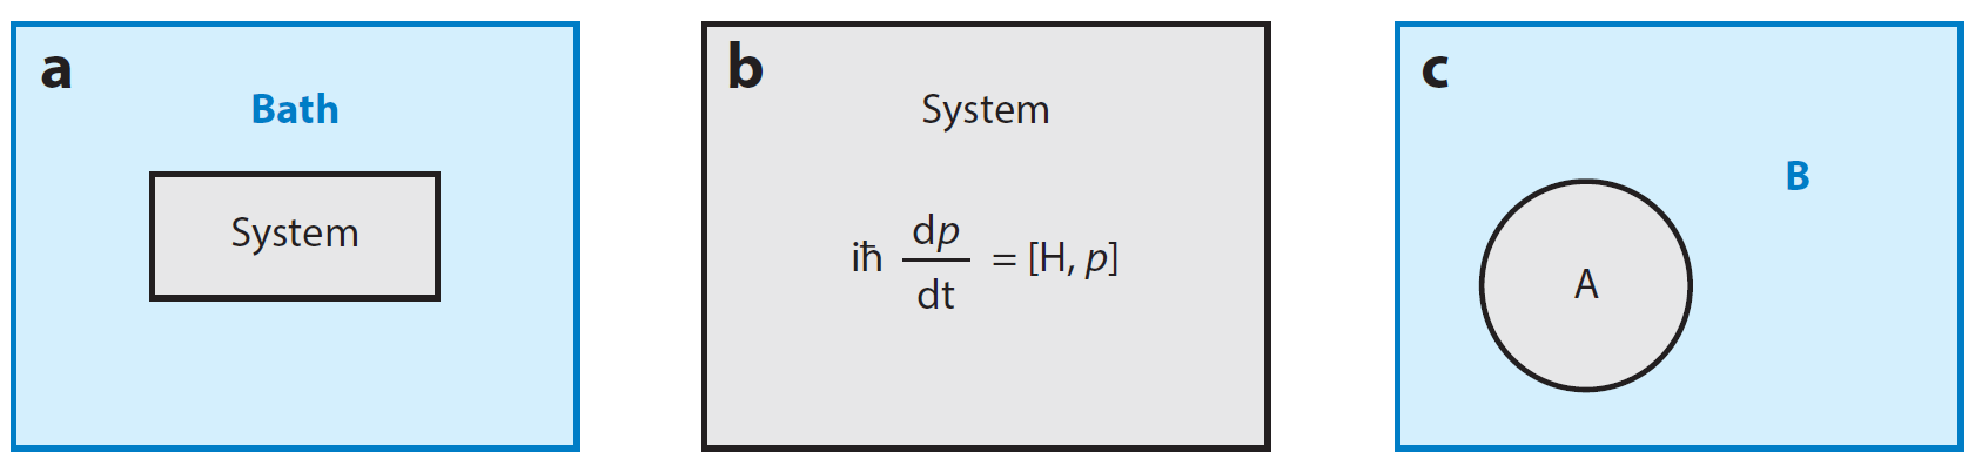
\includegraphics[width=1\textwidth]{nandkishore_huse_reservoir.pdf}}
% \caption{
% \textbf{a)} Pri običajnem kvantnostatističnem opisu sistema privzamemo njegovo sklopitev z zunanjim rezervoarjem, s katerim lahko izmenjuje denimo energijo in delce. \textbf{b)} Tu obravnavamo zaprte oziroma izolirane kvantne sisteme, katerih dinamiko določa unitaren časovni razvoj začetnih stanj. \textbf{c)} Pri obravnavi termalizacije v zaprtih kvantnih sistemih je smiselno sistem razdeliti na podsistema A in B, pri čemer je v A makroskopsko zanemarljiv delež prostostnih stopenj celotnega sistema. V kolikor večji podsistem B manjšemu podsistemu služi kot toplotni rezervoar, je termalizacija možna tudi v zaprtem kvantnem sistemu. Slika je bila vzeta iz Ref.~\cite{nandkishore2015many}. 
% }
% \label{fig:abanin_thermalization}
% \end{figure}
% \end{minipage}
Skupaj z integrabilnimi sistemi predstavljajo MBL sistemi pomemben protiprimer
zgoraj opisani dinamiki ergodičnih sistemov. Dolgočasovni razvoj poljubnega začetnega stanja vodi v ergodičnem in MBL sistemu do povsem različnih rezultatov. Medtem ko pri prvem pričakovane vrednosti lokalnih opazljivk po dolgem času ustrezajo vrednostim ansambelskih povprečij, ki so odvisne le od nekaj dobro definiranih makroskopskih količin, denimo energije in števila delcev, je obnašanje MBL sistemov popolnoma drugačno. `Spomin' na lastnosti začetne konfiguracije se namreč v pričakovanih vrednostih lokalnih opazljivk ohrani tudi po 
neskončnem času. Ker termalizacija poteka prek izmenjave delcev in energije med različnimi deli ergodičnega
sistema, torej preko različnih transportnih mehanizmov, so, v nasprotju s tipično prevodnimi termalizirajočimi sistemi, lokalizirani sistemi izolatorji. V neurejenih sistemih \emph{neinteragirajočih} delcev 
% \begin{minipage}[t]{0.42\textwidth}
% \noindent 
% je tovrstno
% obnašanje dobro poznano~\cite{lagendijk2009fifty}~\cite{abrahams201050} in dolgo preučevano, saj je P.W. Anderson v svojem prelomnem članku~\cite{anderson1958absence} že leta 1958 pojasnil vlogo nereda pri prehodu med prevodnim 
% in izolativnim obnašanjem v preprostem modelu tesne vezi ob prisotnosti naključnih potencialov. Omenjeni mehanizem izogibanja termalizaciji v neinteragirajočih sistemih danes imenujemo \emph{Andersonova lokalizacija}, sistemi, v katerih je realiziran, pa so Andersonovi izolatorji. Ob dovolj močnem potencialnem neredu so vse enodelčne valovne funkcije tovrstnih sistemov lokalizirane, pri čemer njihova verjetnostna gostota pojema eksponentno z razadaljo od neke točke v prostoru. V nasprotju s prostorsko razsežnimi valovnimi funkcijami 
% \end{minipage}\hfill
% \begin{minipage}[t]{0.55\textwidth}
% \begin{figure}[H]
% \centering{
% 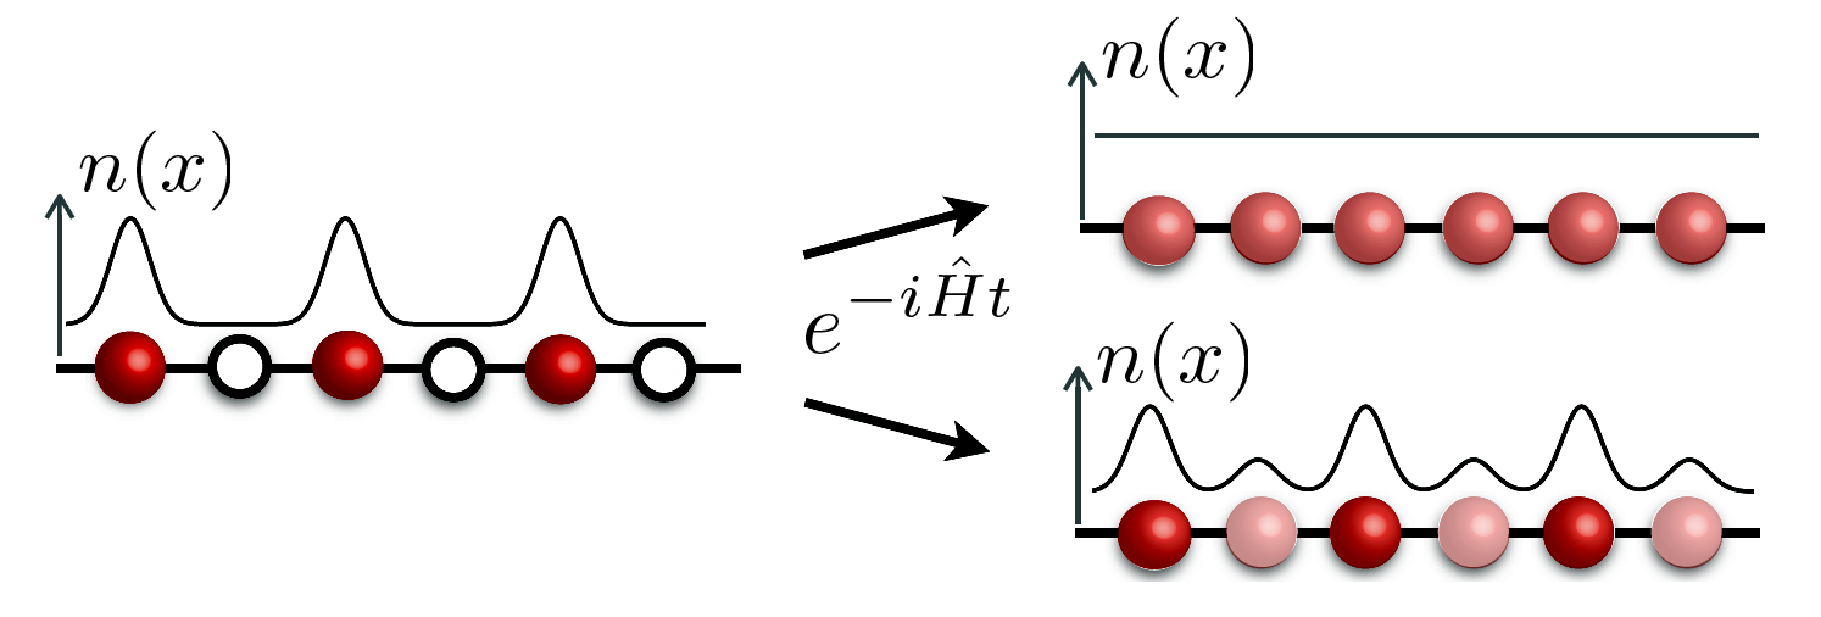
\includegraphics[width=0.95\textwidth]{abanin_thermalization_scheme.pdf}}
% \caption{
% Shematski prikaz razlike med unitarnim časovnim razvojem netipične začetne konfiguracije interagirajočih delcev v ergodičnem in MBL režimu, kjer je netipičnost dosežena z alternirajočo zasedenostjo mest na kristalni verigi.
%  V prvem primeru sistem sčasoma relaksira proti ravnovesni enakomerni porazdelitvi delcev, medtem ko se tovrstna relaksacija v MBL fazi ne zgodi - tudi po dolgem času sistem ohrani spomin na netipičnost začetnega stanja. Slika je bila vzeta iz Ref.~\cite{abanin2018ergodicity}. 
% }
% \label{fig:abanin_thermalization}
% \end{figure}
% \end{minipage}
je tovrstno
obnašanje dobro poznano~\cite{lagendijk2009fifty}~\cite{abrahams201050} in dolgo preučevano, saj je P.W. Anderson v svojem prelomnem članku~\cite{anderson1958absence} že leta 1958 pojasnil vlogo nereda pri prehodu med prevodnim 
in izolatorskim obnašanjem v preprostem modelu tesne vezi ob prisotnosti naključnih potencialov. Omenjeni mehanizem izogibanja termalizaciji v neinteragirajočih sistemih danes imenujemo \emph{Andersonova lokalizacija}, sistemi, v katerih je realiziran, pa so Andersonovi izolatorji. Ob dovolj močnem potencialnem neredu so vse enodelčne valovne funkcije tovrstnih sistemov lokalizirane, pri čemer njihova verjetnostna gostota pojema eksponentno z razadaljo od neke točke v prostoru. V nasprotju s prostorsko razsežnimi valovnimi funkcijami 
lokalizirane 
funkcije ne
 prispevajo k transportu v sistemu in tako preprečujejo termalizacijo. Kot sta točno pokazala Mott in Twose~\cite{doi:10.1080/00018736100101271}, povzroči v eni dimenziji ob odsotnosti meddelčnih interakcij še tako majhen nered nastop Andersonove lokalizacije in odsotnost prevodnosti. Podobno velja v dveh dimenzijah~\cite{abrahams1979scaling}, medtem ko v tridimenzionalnem primeru obstaja kritična vrednost nereda, nad katero imajo sistemi izolativne, pod njo pa prevodne lastnosti~\cite{mott1990metal}. Pri temperaturi nič tako spreminjanje nereda vodi do prehoda med prevodno in lokalizirano fazo. \\\\
 Čeprav je enodelčna lokalizacija zaradi omenjene  vloge dimenzionalnosti pri nastopu lokalizacijskih pojavov že sama po sebi zapletena in zanimiva, odpira vključitev meddelčnih interakcij povsem nove raziskovalne možnosti. Preplet nereda in meddelčnih interakcij odpira vprašanja o možnosti obstoja MBL pri končnih temperaturah~\cite{basko2006metal}~\cite{PhysRevB.75.155111} in o lastnostih meddelčnih interakcij. V zadnjih letih postaja področje vse bolj privlačno ne samo zaradi rezultatov numeričnih analiz~\cite{vznidarivc2008many}~\cite{PhysRevB.75.155111}~\cite{PhysRevA.92.041601}, temveč tudi zaradi porajajočih se možnosti realizacije MBL sistemov v eksperimentih z ultrahladnimi atomi~\cite{PhysRevLett.114.083002}~\cite{schreiber2015observation}~\cite{PhysRevLett.116.140401}. Nekatera izmed odprtih vprašanj s področja so naslovljena tudi v raziskovalnem delu, predstavljenem v magistrski nalogi, kjer se ukvarjamo s prehodom med ergodičnim in MBL režimom v kvantnomehanskem modelu $t$-$J$~\cite{spalek2007tj}. Pri preučevanju nastopa lokalizacije me zanima vloga različnih tipov nereda, posebej primerjava med vplivom nereda, ki se sklaplja s spinskimi prostostnimi stopnjami, in nereda, ki se sklaplja s prostostnimi stopnjami nosilcev naboja. Način vpeljave obeh zvrsti nereda podrobneje razložim v nadaljnjih poglavjih ob formalni predstavitvi modela.
  \\\\Raziskovalno delo temelji na numeričnih metodah, točneje polni diagonalizaciji modelskih hamiltonk in 
  analizi tako izračunanih spektrov.  Različne spektralne lastnosti hamiltonk ergodičnih in MBL modelskih sistemov izkoriščam pri analizi na podlagi teorije naključnih matrik~\cite{d2016quantum} (ang.~\emph{random matrix theory}, v nadaljevanju RMT), v okviru katere so podane teoretične napovedi~\cite{mehta2004random} za vrednosti različnih spektralnih statistik in opazljivk, s katerimi primerjamo svoje izračune. Med omenjenimi statistikami sta posebej izpostavljena povprečen razmik med sosednjimi nivoji in statistika razmikov sosednjih energijskih nivojev~\cite{Atas_Distribution_PhysRevLett.110.084101}~\cite{PhysRevB.75.155111}. Slednji sta zaradi sorazmerne enostavnosti implementacije pogosto uporabljani za presojo ergodičnosti oziroma lokaliziranosti sistema. Ker vsebujeta informacije zgolj o korelacijah med najbližjimi energijskimi nivoji v spektru, podajata obnašanje modelskih sistemov na najdaljših časovnih skalah. Polnejši vpogled v dogajanje na vseh časovnih skalah sistemov dobimo z izračunom spektralnega oblikovnega faktorja (ang.~\emph{spectral form factor}, v nadaljevanju SFF) oziroma Fourierove transformacije dvotočkovne korelacijske funkcije energijskega spektra. Izsledke metod, ki temeljijo na statističnih lastnostih energijskih spektrov, dopolnimo in primerjamo z izračuni prepletenostne entropije vseh lastnih stanj modelskih hamiltonk. Znanilec nastopa MBL je v tem primeru `površinsko skaliranje' prepletenostne entropije v odvisnosti od velikosti podsistema v nasprotju s `prostorninskim skaliranjem' v ergodičnih sistemih. \\\\
  Na začetku drugega poglavja najprej podrobneje predstavimo pojav Andersonove lokalizacije v neurejenih sistemih neinteragirajočih delcev in razložimo pomen različnih modelov nereda. Nato prek dodatka meddelčnih interakcij obravnavo razširimo na področje MBL. V tretjem poglavju predstavimo tipične modelske sisteme, primerne za preučevanje nastopa MBL, in sicer Heisenbergovo verigo, Hubbardov model in model $t$-$J$, ki ima osrednjo vlogo v raziskovalnem delu, predstavljenem v tej magistrski nalogi. Poleg modelov predstavimo tudi numerično implementacijo točne diagonalizacije. V četrtem poglavju predstavimo statistične lastnosti hamiltonskih spektrov in vpeljemo ključne pojme s področja RMT. Predstavljeni so rezultati analize sosednjih energijskih nivojev v odvisnosti od različnih tipov nereda in rezultati analize SFF. Peto poglavje je namenjeno vpeljavi prepletenostne entropije in predstavitvi izračunov za to količino. 




%ne sme manjkati: kaj so še razlike: poleg zloma ergodičnosti in odsotnosti transporta je tu še spektralna statistika in prepletenostna entropija -> to mi študiramo. Potem lahko pride na vrsto že predstavitev vsebine po poglavjih. 
%sistem pripravljen v neravnovesnem stanju -> kaj se zgodi - > lahko termalizira, lahko pa ne; ETH ne ubogajo MBL 
%integrabilni sistemi -> MBL: vanishing transport 

%KLJUČNE TEME: 
%MBL
%TERMALIZACIJA, EKVILIBRACIJA, VLOGA NEREDA
%
%NAVEŽI SE TUDI NA SEMINAR IN ANDERSONA
% Kaj navesti: glej: MBL and thermalization in disordered Hubbard chains (Rigol, Mondaini) - naštej, zakaj je to pomembno, od kdaj je to zanimivo in kateri članki pridejo v poštev -> 
% vloga nereda v sistemu -> vpelješ, glej Abanin => začneš z Andersonom, omembo prelomnega članka (1958), tu se lahko nanašaš na seminar. Sicer večino teksta pri seminarju pride v poštev v naslednjem podpoglavju
% v uvodu: obvezno slika Abanin (kaj je to lokalizacija, kaj je značilnost sistema, kako je s termalizacijo). Glej Nandkishore, Huse za razlago, kaj je MBL in zakaj je pomemben
% MBL represents a new frontier of quantum statistical mechanics. MBL systems fail to thermally equilibrate, so their long-time states are not captured by conventional equilibrium statistical mechanics ... 
\chapter{Od Andersonove do večdelčne lokalizacije}
\section{Andersonova lokalizacija in osnove neurejenih sistemov}
\label{anderson}
Obravnavo lokalizacijskih pojavov začnemo z vpeljavo pojma Andersonove lokalizacije, ki nastopi v neurejenih sistemih neinteragirajočih delcev. Razumevanje mehanizmov, ki vodijo do lokalizacije ob odsotnosti interakcij, je namreč dobrodošla osnova za razširitev obravnave z dodatkom meddelčnih interakcij in posledično preučevanje MBL pojavov. \\\\	
Zaradi translacijske simetrije lahko v idealno urejenih kristalnih strukturah elektronske valovne funkcije  opišemo kot prostorsko razsežne Blochove valovne funkcije. Stanja dejanskih sistemov se pogosto bistveno razlikujejo od tovrstnega idealiziranega opisa, saj je zaradi tako rekoč neizogibne prisotnosti nečistoč, defektov in vrzeli idealna kristalna urejenost v praksi le bolj ali manj dobra predpostavka. Pri tem se v razpravi o neurejenih sistemih uporabljan pojem \emph{nereda} nanaša na vsa omenjena odstopanja od idealne urejenosti.  V limiti majhnega nereda, ko se odstopanja od sicer popolne ureditve pojavijo le na nekaj mestih, so valovne funkcije sistema še vedno prostorsko razsežne in le malo odstopajo od ravnih valov. Z naraščanjem nereda se lahko njihova narava popolnoma spremeni, saj lahko nekatere  postanejo lokalizirane z eksponentno pojemajočo ovojno funkcijo, kot prikazuje Slika~\ref{fig:dif_loc_ext}. \\\\Elektroni z lokaliziranimi valovnimi funkcijami so znotraj sistema omejeni na končna območja in zato zanemarljivo malo vplivajo na transportne lastnosti, medtem ko elektroni zasedajoč prostorsko razsežna stanja tipično prispevajo h končnemu transportu. Posledično je sistem izolator, če pod njegovo Fermijevo energijo obstajajo zgolj lokalizirana stanja, in prevodnik, v kolikor Fermijev nivo sovpada z energijo prostorsko razsežnih stanj~\cite{kramer1993localization}. Za razlago obstoja prevodnikov in izolatorjev in razlik med njimi je torej ključno razumevanje vloge nereda pri lokalizaciji kvantnomehanskih valovnih funkcij. Poleg vpliva količine nereda in dimenzionalnosti sistema so v tem podpoglavju razloženi tudi osnovni pojmi s področja Andersonove lokalizacije. V magistrski nalogi se pojem lokalizacija  nikoli ne nanaša na t.i. Mottovo lokalizacijo,
ki je posledica močnih odbojnih medelektronskih interakcij in je v nalogi ne obravnavamo. \\\\
\begin{minipage}[t]{0.54\textwidth}
\noindent 
 Možnost lokalizacije elektronskih valovnih funkcij ob prisotnosti dovolj močnega potencialnega nereda je leta 1958 prvi napovedal P.W. Anderson~\cite{anderson1958absence}. Medtem ko sta limitna primera šibkega in močnega nereda intuitivno razmeroma lahko predstavljiva, je bilo vprašanje o obnašanju sistemov v vmesnem režimu, posebej v dveh dimenzijah, dolgo časa odprto. Mott in Twose sta za enodimenzionalne sisteme eksaktno dokazala~\cite{doi:10.1080/00018736100101271} nastop lokalizacije ob prisotnosti vsakršnega končnega nereda, enak rezultat pa  v termodinamski limiti neskončnih sistemov velja tudi v dveh dimenzijah~\cite{abrahams1979scaling}. Kot je leta 1968 pokazal Mott, obstaja v treh dimenzijah kritična 
\end{minipage}\hfill
\begin{minipage}[t]{0.42\textwidth}
\begin{figure}[H]
\centering{
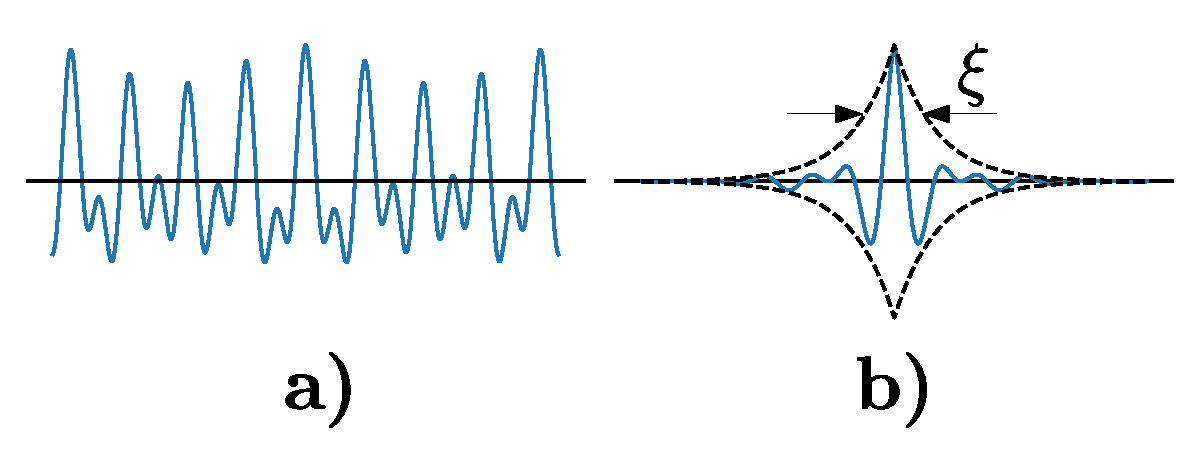
\includegraphics[width=0.95\textwidth]{diff_loc_ext_mod.pdf}}
\caption{Teorija Andersonove lokalizacije napove možnost lokalizacije kvantnomehanskih stanj zaradi naključnih potencialov. \textbf{a)} Primer razsežnega stanja. \textbf{b)} Lokalizirano stanje, katerega ovojnica eksponentno pojema z razdaljo od neke točke v prostoru. $\xi$ je lokalizacijska dolžina. 
}
\label{fig:dif_loc_ext}
\end{figure}
\end{minipage}\\
   energija $E_c$ oziroma \emph{rob mobilnosti}~\cite{mott1990metal}, ki loči lokalizirana od razsežnih stanj. Energija prvih je manjša, drugih pa večja od kritične energije $E_c$. Obstoj roba mobilnosti danes označuje nastop z neredom vzbujenega faznega prehoda med kovino in izolatorjem. Leta 1977, manj kot 20 let po objavi prelomnega članka, je bila Andersonu za njegovo delo podeljena Nobelova nagrada za fiziko~\cite{anderson1978local}.
 \subsection{Opis prevodnosti pred teorijo lokalizacije in po njej}  
 Lokalizacija kvantnomehanskih delcev v naključnih potencialih je zanimiv statističnofizikalni pojav. Pred razvojem teorije Andersonove lokalizacije so za opis elektronske prevodnosti tipično uporabljali kvantnomehansko različico Drudejevega modela. Pri slednjem privzamemo sorazmernost prevodnosti s \emph{povprečno prosto potjo} $l$, torej razdaljo, ki jo delec v snovi prepotuje pred trkom z nečistočo. V kvantnomehanskem smislu to pomeni, da se valovni paketi pri propagaciji vzdolž neurejenega medija na naključnem potencialu v povprečju sipajo po prepotovani razdalji $l$. Čeprav zaradi sipanja na naključnem potencialu valovni paketi nimajo več ostro določenega valovnega vektorja, ostanejo valovne funkcije sipanju navkljub prostorsko razsežne. Na daljših razdaljah je tovrstna propagacija skozi medij difuzivna, povečanje količine nereda v sistemu pa vodi do zmanjšanja povprečne proste poti. Zaradi predpostavke sorazmernosti med prevodnostjo in povprečno prosto potjo Drudejev model pri nobenem končnem neredu ne napove ničelne prevodnosti. Napovedi modela so bile v nasprotju s presenetljivo dolgimi relaksacijskimi časi elektronskih spinov, izmerjenimi v poskusih z dopiranimi polprevodniki, ki jim je v petdesetih letih v Bellovih laboratorijih prisostvoval Anderson~\cite{lagendijk2009fifty}~\cite{anderson1978local}. V nasprotju z Drudejevim modelom rezultate uspešno razloži model, v katerem valovne funkcije pri dovolj močnem neredu postanejo lokalizirane z eksponentno pojemajočo ovojnico, $\left|\psi\left(\textbf{r}\right)\right|   \sim \exp\left(\left|\textbf{r}- \textbf{r}_0\right|\right/\xi)$, kjer je $\xi$ \emph{lokalizacijska dolžina}. V kolikor so vse valovne funkcije lokalizirane, se dizufivna propagacija v neurejenem mediju ne samo upočasni, temveč popolnoma ustavi - delci postanejo ujeti, prevodnost pa pade na ničelno vrednost~\cite{wolfle2010self}. Presenetljiv rezultat je možno razložiti preko obravnave večkratne interference valovnih komponent, sipanih na naključno porazdeljenih sipalcih - lokalizacija je namreč v svojem bistvu interferenčni pojav. 
 \subsection{Ojačano povratno sipanje}
 Pomen interferenčnih pojavov pri nastopu Andersonove lokalizacije je vsaj intuitivno najlažje razložiti z uporabo osnovnih načel valovne mehanike. Privzemimo limito šibkega nereda in obravnavajmo delec, ki se v neurejenem mediju propagira med točkama $\textbf{r}_0$ in $\textbf{r}_1$. Za izračun verjetnosti delčevega prihoda v točko $\textbf{r}_1$ moramo sešteti vse kompleksne verjetnostne amplitude različnih poti med točkama in izračunati kvadrat absolutne vrednosti končne vsote. Verjetnost na koncu podajata vsota kvadratov posameznih verjetnostnih amplitud ter vsota mešanih, interferenčnih členov. Prva ustreza klasičnemu nekoherentnemu prispevku, drugo pa lahko v večini primerov upravičeno zanemarimo zaradi predpostavke naključne porazdelitve faz interferenčnih členov v neurejenem mediju. Z neupoštevanjem interferenčnih členov dobimo namesto napovedi lokalizacije Drudejev opis prevodnosti v neurejenih sistemih, torej očitno obstajajo primeri, v katerih interfenčnih členov ne smemo zanemariti. \\\\
 \begin{minipage}[t]{0.55\textwidth}
\noindent  
Naj bo delec uvodoma v točki $\mathbf{r}_0$ in naj bo $A_1$ verjetnostna amplituda za proces, v katerem se delec vzdolž neke poti $C_1$ vrne v izhodiščno točko, $A_2$ pa naj bo amplituda povratka v izhodiščno točko vzdolž neke druge poti $C_2$, kot prikazuje Slika~\ref{fig:paths}.
Skupno verjetnost povratka podaja zveza 
\begin{equation}
w=|A_1 + A_2|^2=w_\mathrm{cl} + w_\mathrm{int},
\end{equation}
kjer je $w_\mathrm{cl}=|A_1|^2 + |A_2|^2$ in $w_\mathrm{int}=2\Re\left(A_1^*A_2\right)$ \cite{wolfle2010self}. Za različni poti $C_1$ in $C_2$ se interferenčni členi v povprečju izničijo in je njihovo neupoštevanje upravičeno. Drugače je v posebnem primeru, ko je  $A_2=A_r$ verjetnostna amplituda za proces, v katerem povratek poteka vzdolž poti 
\end{minipage}\hfill
\begin{minipage}[t]{0.41\textwidth}
\begin{figure}[H]
\centering{
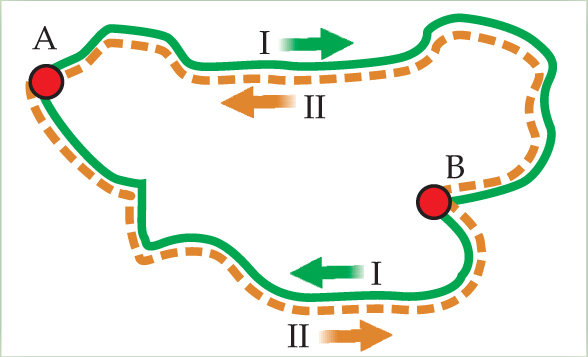
\includegraphics[width=0.9\textwidth]{interference.jpg}}
\caption{Shematski prikaz valovnega paketa, ki se preko poti I skozi točko B vrne v izhodično točko A. Pot II je enaka poti I, le da je obrnjena v času. Slika je bila vzeta iz \cite{lagendijk2009fifty}.}
\label{fig:paths} 
\end{figure}
\end{minipage}
$C_1$, vendar v obratni smeri. V kolikor je sistem simetričen na obrat 
časa, $A_1=A_r$, potem s pravilnim upoštevanjem interferenčnih  členov izračunamo dvakrat večjo verjetnost povratka kot v klasičnem primeru: 
\begin{equation}
w=4\left|A_1\right|^2=2w_\mathrm{cl}.
\end{equation}
Zaradi konstruktivne interference poti z njeno v času obrnjeno ustreznico je torej pri sipalnem dogodku verjetnost za povratno sipanje v izhodiščno točko večja od verjetnosti vseh preostalih izidov dogodka. Pojav imenovan \emph{ojačano povratno sipanje} zmanjša transmitivnost medija in posledično zmanjša tudi njegovo prevodnost. \newpage
\subsection{Skalirna teorija lokalizacije}
Lokalizacija v neurejenih sistemih je netrivialno odvisna od njihove dimenzionalnosti. Medtem ko v eni dimenziji vsakršnen končni nered povzroči lokalizacijo vseh valovnih funkcij, obstaja v treh dimenzijah kritična vrednost nereda, nad katero so vsa stanja lokalizirana, za podkritične vrednosti nereda pa v sistemu soobstajajo razsežna in lokalizirana stanja. Medtem ko za dvodimenzionalne sisteme~\cite{kramer1993localization} rigorozen dokaz ne obstaja se zdi, da so v termodinamski limiti neskončnega sistema vse valovne funkcije lokalizirane pri vsakršni končni vrednosti nereda, podobno kot v enodimenzionalnem primeru. Za razliko od neskončnih sistemov lahko končni dvodimenzionalni sistemi kažejo prevodne lastnosti. \\\\ 
Opisana zapletena vloga dimenzionalnosti pri nastopu lokalizacijskih pojavov je danes pogosto razložena v okviru \emph{skalirne teorije} lokalizacije, ki so jo leta 1979 razvili Abrahams, Anderson, Licciardello in Ramakrishnan~\cite{abrahams1979scaling}. Navkljub svoji preprostosti in fenomenološkemu pristopu teorija pravilno napove glavne lastnosti lokalizacije v različnih dimenzijah in tako ob odsotnosti rigoroznega teoretičnega modela ponuja dragocen uvid v značilnosti lokalizacijskih pojavov. Skalirna teorija opisuje Andersonovo lokalizacijo v jeziku kritičnih fenomenov zveznih kvantnih faznih prehodov. Slednji nastopijo pri ničelni temperaturi in jih namesto temperature vodi spreminjanje nekega drugega parametra - v primeru lokalizacijskih pojavov je to količina nereda v sistemu. Ker gre za teorijo faznih prehodov, skalirna teorija za različne količine napove skalirne zakone. Tu bo na kratko predstavljena le skalirna zveza za specifično prevodnost.\\\\
Pred nadaljevanjem se spomnimo, da sta v tridimenzionalnem ohmskem prevodniku prevodnost $g$ in specifična prevodnost $\sigma$ povezani z zvezo $g=\sigma\frac{S}{L}.$ Pri tem je $S$ prečni presek prevodnika in $L$ njegova dolžina. Pri skalirni teoriji v splošnem obravnavamo odvisnost prevodnosti $d$-dimenzionalne hiperkocke od dolžine njene stranice $L$, zato uvedemo logaritemski odvod $\beta$ kot 
\begin{equation}\label{eq:beta_log}
\beta=\frac{\dd \log g}{\\d \log L}.
\end{equation}
Teorija privzame eksplicitno odvisnost $\beta$ zgolj od $g$, ne pa tudi od energije, nereda ali dolžine stranice $L$. Kvalitativno obnašanje količine $\beta$ določata znani asimptotski limiti majhne in velike prevodnosti, medtem ko so vmesne vrednosti določene z interpolacijo ob predpostavki, da je $\beta$ zvezna in monotono naraščajoča funkcija. \\\\
Iz En. \eqref{eq:beta_log} je očitno naraščanje $g$ z velikostjo sistema v primeru $\beta>0$, kar označuje kovinski oziroma prevoden značaj, v katerem velja dobro poznana klasična zveza med prevodnostjo in specifično prevodnostjo,
\begin{equation}\label{eq:g_prevodnik}
g(L)=\sigma\frac{L^{d-1}}{L}=\sigma L^{d-2}.
\end{equation}
Zgoraj zapisana zveza za ohmski prevodnik je le poseben primer En.~\eqref{eq:g_prevodnik}, ki nam v prevodnem območju da zvezo $\beta=d-2$. Posledično je količina $\beta$ pozitivna le za tridimenzionalne prevodnike, ničelna v dveh in negativna v eni dimenziji. V nasprotni, torej lokalizirani limiti, $g$ pojema eksponentno z velikostjo sistema, $g\propto \exp(-L)$ in $\beta<0$. \\
\noindent
\begin{minipage}[t]{0.44\textwidth}
% Iz En. \eqref{eq:beta_log} je očitno naraščanje $g$ z velikostjo sistema v primeru $\beta>0$, kar označuje kovinski oziroma prevoden značaj, v katerem velja dobro poznana klasična zveza med prevodnostjo in specifično prevodnostjo,
% \begin{equation}\label{eq:g_prevodnik}
% g(L)=\sigma\frac{L^{d-1}}{L}=\sigma L^{d-2}.
% \end{equation}
Dejanska funkcijska odvisnost je v lokaliziranem režimu podana z zvezo 
\begin{equation}
\beta=\frac{\dd \log g}{\dd L}\frac{\dd L}{\dd \log L}=\log g
\end{equation}
 Prehod med izolatorjem in prevodnikom se zgodi v kritični točki $\beta(g_c)=0$. To je možno zgolj v treh dimenzijah, kjer $\beta$ zavzame tako negativne kot pozitivne vrednosti. V nižjih dimenzijah prevodnost z naraščanjem velikosti sistema vedno pada in tako kritična točka ni nikoli dosežena. Razlika med tridimenzionalnim in nižjedimenzionalnima primeroma je shematsko prikazana na Sliki~\ref{fig:scalingtheory}.
\end{minipage}\hfill
\begin{minipage}[t]{0.5\textwidth}
\begin{figure}[H]
\centering{
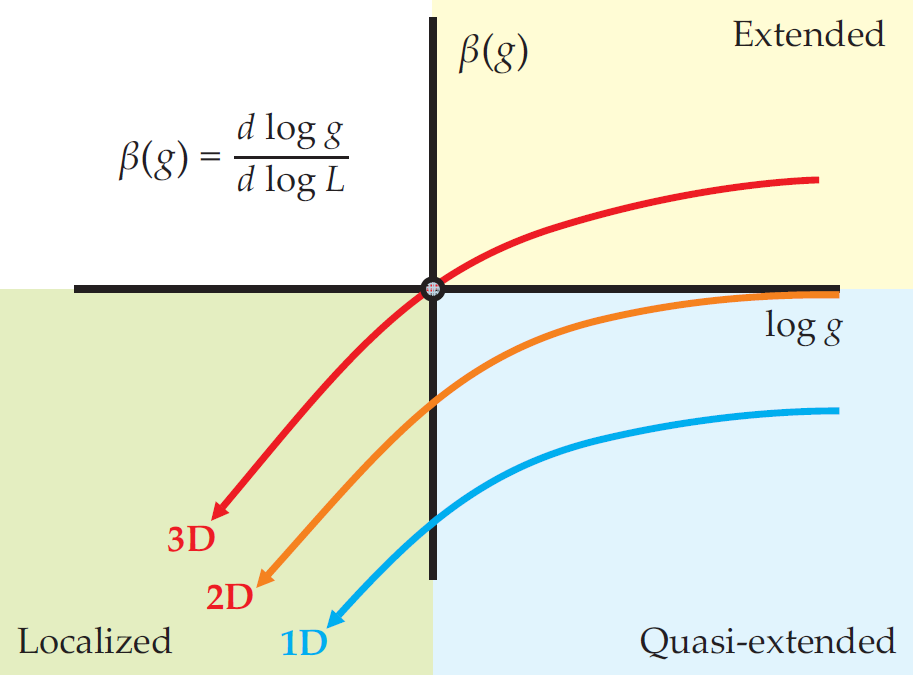
\includegraphics[width=0.8\textwidth]{beta_diagram.png}}
\caption{Skalirna teorija napove fazni prehod med prevodnikom in izolatorjem le v treh dimenzijah, saj v nižjedimenzionalnih sistemih prevodnost z velikostjo sistemov vselej pada. Slika je bila vzeta iz~\cite{lagendijk2009fifty}.}
\label{fig:scalingtheory} 
\end{figure}
\end{minipage}\\\\
\vspace{1cm}
\subsection{Vpeljava nereda in Andersonov model}
V tem podpoglavju predstavimo različne modele nereda v kvantnomehanskih sistemih. Podana je razlaga uvedbe nereda v idealno urejene kristalne sisteme, kot najpogosteje uporabljan model neurejenega sistema neinteragirajočih delcev pa je podrobneje predstavljen Andersonov model. \\\\
Opis translacijsko invariantnih sistemov je zaradi njihove translacijske simetrije razmeroma enostaven. Enoelektronske valovne funkcije so v teh sistemih Blochovega tipa, posledično so elektroni prosto gibljivi. V večini dejanskih sistemov je idealna translacijska simetrija zlomljena zaradi prisotnosti nereda, ki lahko bistveno vpliva na fizikalne lastnosti sistemov. V primeru nizke koncentracije defektov lahko pri opisu neurejenih sistemov kot izhodišče uporabimo koncepte, veljavne v translacijsko invariantnih sistemih. Na drugi strani velika koncentracija defektov terja popolno opustitev predpostavke translacijske simetrije in uporabo novih pristopov. \newpage
\noindent
\begin{minipage}[t]{0.54\textwidth}
Kot prikazuje Slika~\ref{fig:disorder_scheme}, lahko različne modele nereda dobimo s takšno ali drugačno deformacijo idealne kristalne strukture. Modele za opis \emph{strukturno neurejenih} sistemov, kot so npr. amorfni polprevodniki,  dobimo z naključnimi premiki delcev z mest na urejeni kristalni rešetki. Enodelčno hamiltonko takšnega sistema podaja 
\begin{equation}\label{eq:cont_ham}
H=\frac{p^2}{2m} + \sum\limits_{j=1}^N U_j(\textbf{r}- \textbf{R}_j), 
\end{equation}
kjer je $p$ operator gibalne količine, $m$ efektivna masa delca, $U_j$ pa potencialna energija atoma na mestu $\textbf{R}_j$. Nered vpeljemo z naključno izbiro potencialnih energij in položajev $\textbf{R}_j$, kjer vrednosti žrebamo v skladu z nekima izbranima normaliziranima verjetnostnima porazdelitvama. \\\\
\end{minipage}\hfill
\begin{minipage}[t]{0.43\textwidth}
\begin{figure}[H]
\centering{
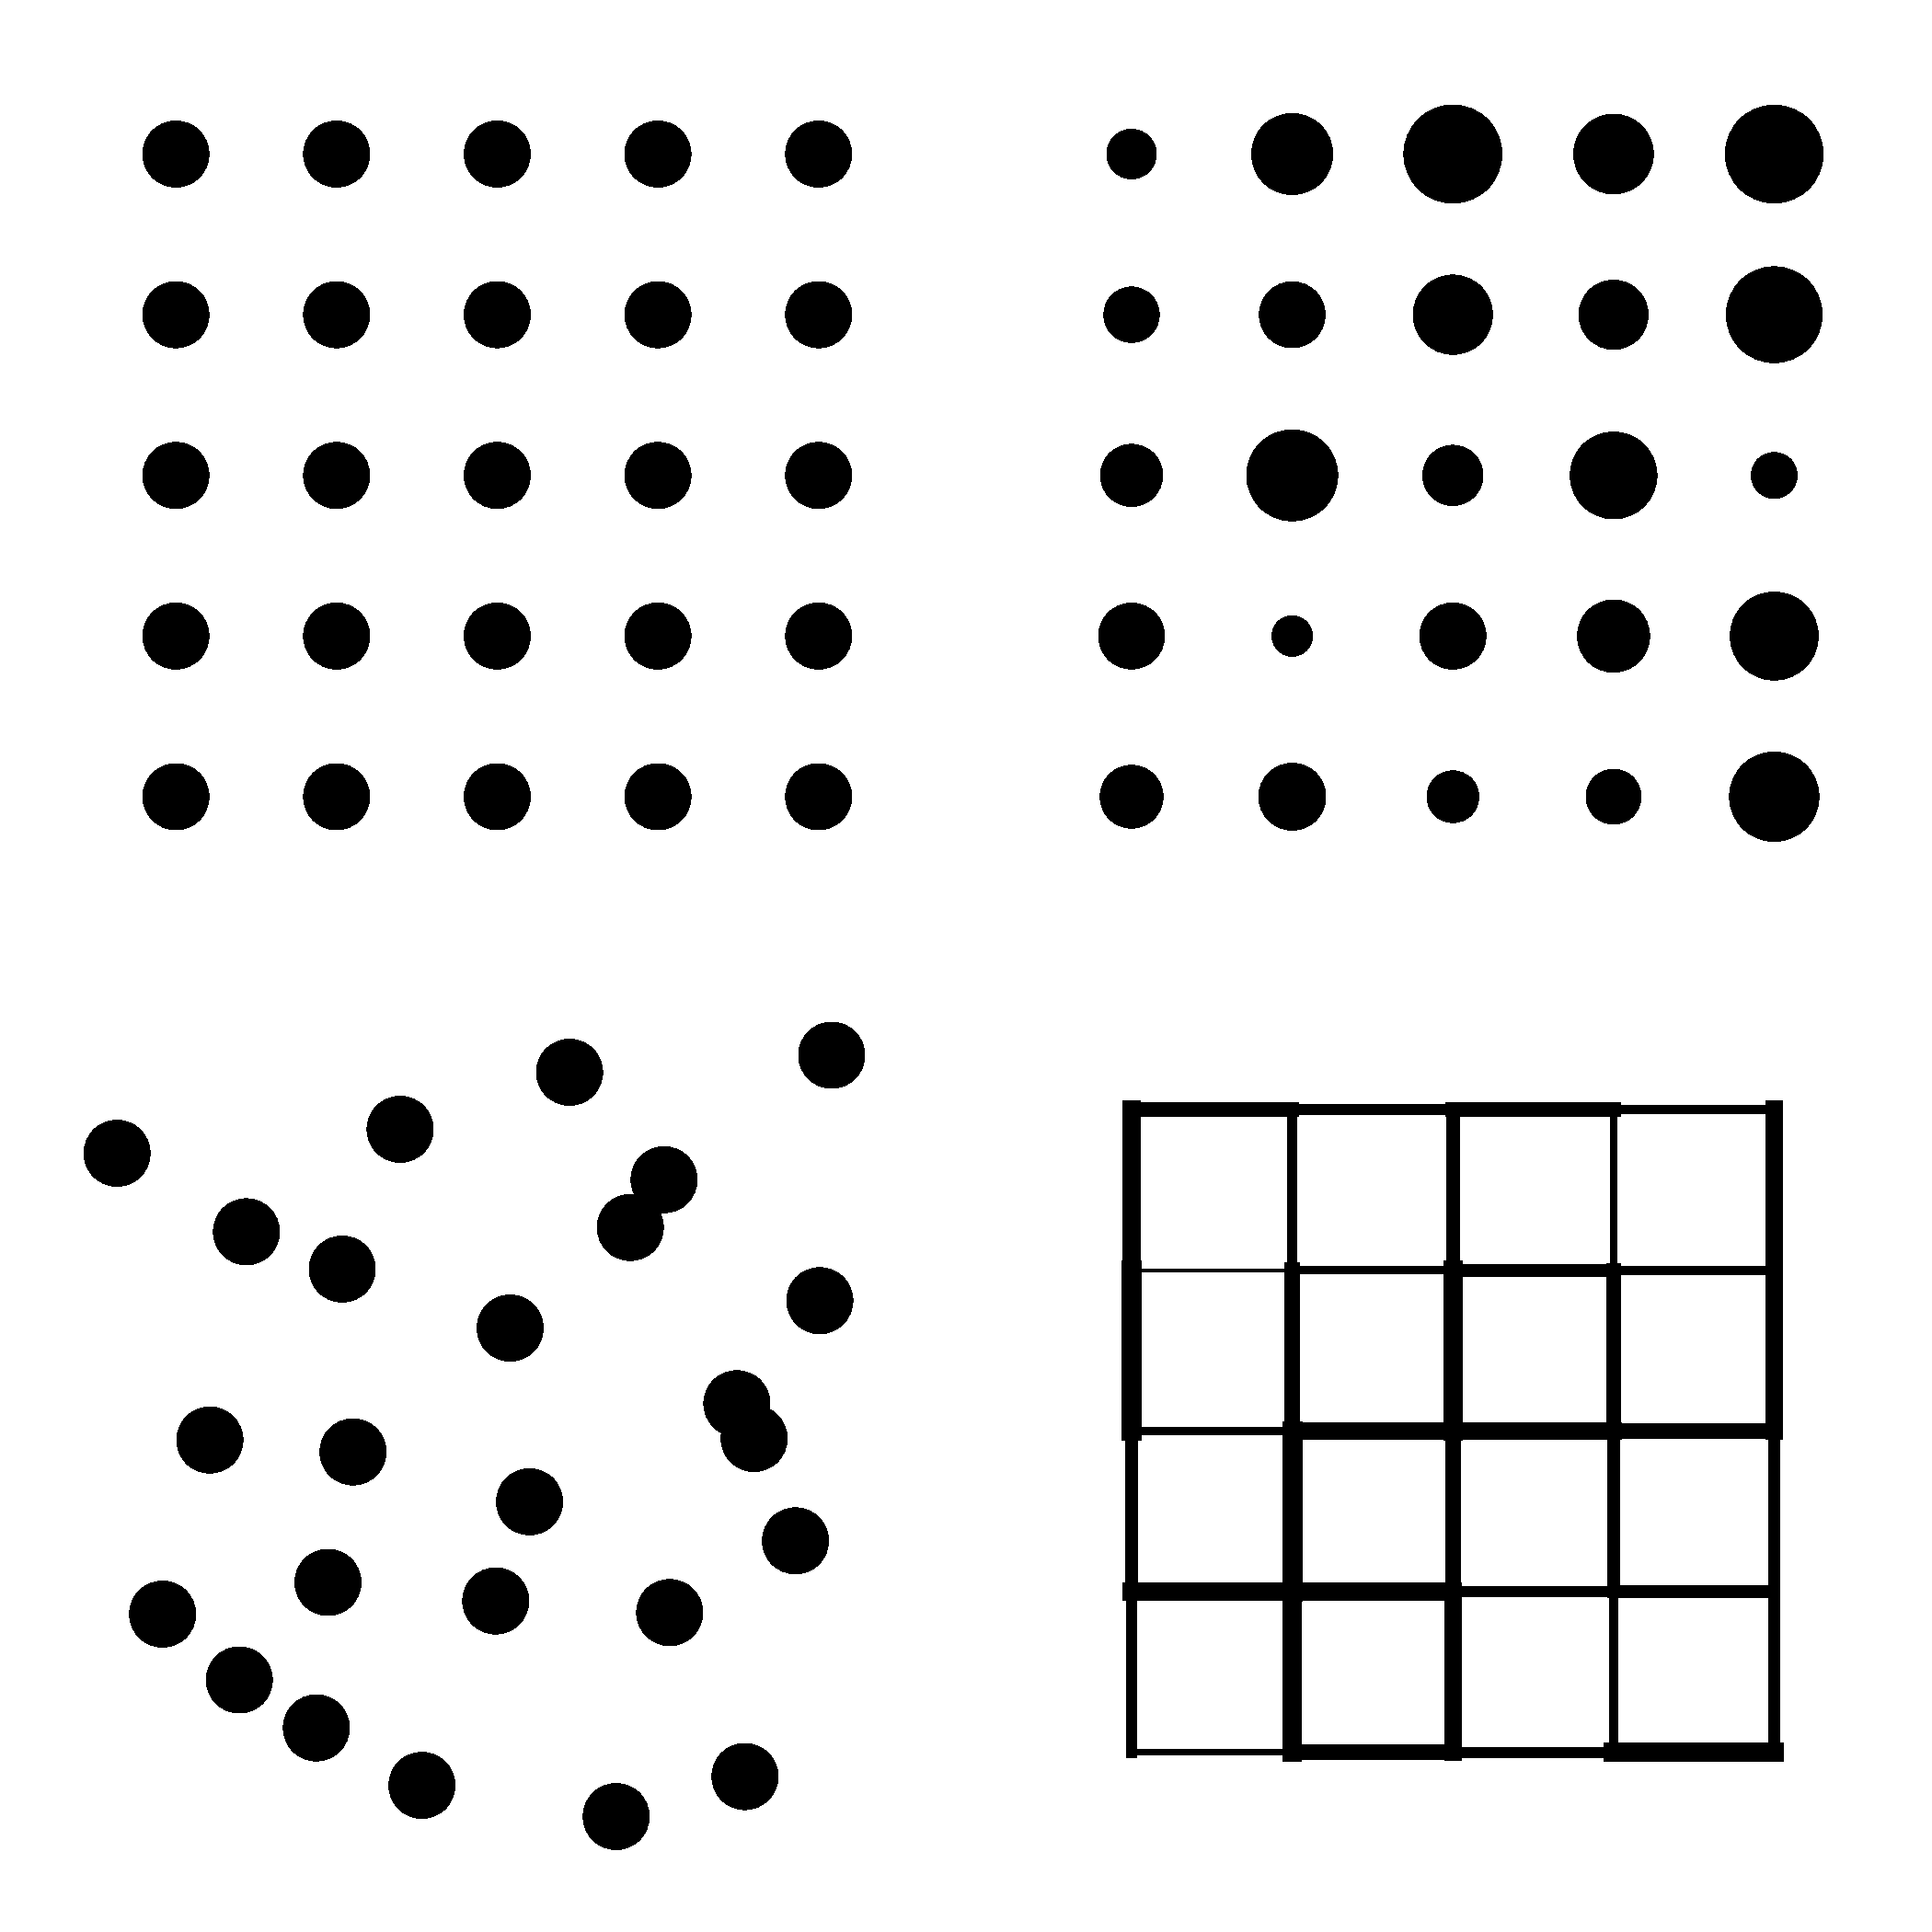
\includegraphics[width=0.8\textwidth]{disorder_scheme.pdf}}
\caption{Od leve proti desni in od zgoraj navzdol so razzvrščeni shematski prikazi idealnega kristala, kompozicijsko neurejenega sistema, strukturno neurejenega sistema in sistema s kinetičnim neredom.  }
\label{fig:disorder_scheme} 
\end{figure}
\end{minipage}
\emph{Kompozicijsko neurejene} sisteme, ki so tudi osrednji predmet preučevanja v magistrski nalogi, najpogosteje opiše hamiltonka v približku tesne vezi na diskretni mreži:
\begin{equation}\label{eq:disc_ham}
H=\sum\limits_{j\nu}u_{j\nu}c^\dagger_{j\nu}c_{j\nu} + \sum\limits_{j\nu, k\mu} t_{j\nu, k\mu} c^\dagger_{j,\nu}c_{k\mu}.
\end{equation}
Tu so $c^\dagger_{j\nu}, c_{j\nu}$ fermionski kreacijski in anihilacijski operatorji za mesto $j$ v kristalni rešetki in stanje $\nu$. Z $u_{j\nu}$ so v diagonalnem delu označene potencialne energije stanj na danih mestih v kristalni rešetki, medtem ko izvendiagonalni matrični elementi $t_{j\nu, k\mu}$ ustrezajo tunelskim prehodom med stanji na različnih mestih na mreži. Nered je vpeljan preko naključnih vrednosti potencialnih členov $u_{j\nu}$ ali \emph{skakalnih} (ang.~\emph{hopping}) členov $t_{j\nu, k\mu}$, kjer pri žrebanju vrednosti ponovno privzamemo neko verjetnostno porazdelitev. V nasprotju z modelom, ki ga podaja En.~\eqref{eq:cont_ham}, tu ni strukturnega nereda, saj so mesta v kristalni rešetki dobro definirana in sovpadajo z mesti urejene kristalne mreže. Pri vseh diskretnih modelih, obravnavanih v magistrski nalogi, bomo medmrežni razdalji $a$ priredili enotsko vrednost, $a=1.$ \\\\
\textbf{Andersonov model}~\cite{anderson1958absence} je poseben primer modela, ki ga podaja En.~\eqref{eq:disc_ham}. Dobimo ga z upoštevanjem predpostavk izključno diagonalnega prispevka k neredu, skakanja elektronov zgolj med najbližjimi sosedi s konstantnim prekrivalnim integralom za tuneliranje $t$ in prisotnostjo le ene orbitale, $\nu=1$. Naključne potencialne energije $u_j$ so porazdeljene enakomerno na intervalu $\left[-W,W\right]$ v skladu s porazdelitvijo
\begin{equation}\label{eq:and_prob}
p(u_j)= \frac{1}{2W}\Theta \left(W - \abs{u_j} \right),
\end{equation}
kjer je $W$ \emph{parameter velikosti nereda}. Hamiltonka Andersonovega modela se tako zapiše kot 
\begin{equation}\label{eq:Anderson_ham}
H=\sum\limits_j u_j n_j + t\sum\limits_{\mathrm{n. s.}}\left(c^\dagger_i c_j + \mathrm{h.c.}\right),
\end{equation}
kjer je $n_j=c^\dagger_jc_j$ operator številske gostote delcev na $j$-tem mestu kristalne mreže.\\\\
\begin{minipage}[t]{0.55\textwidth}
V Andersonovem modelu lahko delec na urejeni mreži skače med sosednjimi mesti z naključno porazdeljenimi potencialnimi energijami, kar shematsko prikazuje Slika~\ref{fig:hopping_picture}. Andersonov model pogosto služi kot izhodišče za konstrukcijo modelov MBL sistemov, o čemer se bomo prepričali pri njihovi obravnavi v poglavju~\ref{modelimetode}.\\\\
Ob odsotnosti nereda je Andersonova hamiltonka običajna hamiltonka v približku tesne vezi, ki opisuje urejeno mrežo enakih potencialnih jam, ki je prikazana na shemi \textbf{a)} na Sliki~\ref{fig:band_structure}.  V tem primeru jo diagonaliziramo z uporabo Fourierove transformacije in pri izračunu spektra dobimo energijski pas širine $2zt$, kjer je $z$ koordinacijsko število kristalne rešetke. Hamiltonko Andersonovega modela dobimo z naključnim spreminjanjem globin posameznih potencialnih jam za vrednosti $U_j$, ki so porazdeljene v skladu s porazdelitvijo, ki jo podaja En.~\eqref{eq:and_prob}. Kot prikazuje shema \textbf{b)} na Sliki~\ref{fig:band_structure}, dodatek nereda razširi energijski pas in odpravi singularnosti v gostoti stanj, ki so sicer značilne za sisteme z redom dolgega dosega. \\\\
V limiti zelo močnega nereda, kjer velikost parametra nereda $W$ primerjamo s hitrostjo tuneliranja $t$, lahko privzamemo, da potencialni člen v En.~\eqref{eq:Anderson_ham} močno prevlada nad izvendiagonalnim skakalnim členom in tako povzroči lokalizacijo valovnih funkcij. V okviru perturbacijske teorije lahko lastne funkcije hamiltonke opišemo kot vezana stanja ali orbitale, ki postanejo lokalizirane zaradi 
\end{minipage}\hfill
\begin{minipage}[t]{0.4\textwidth}
\begin{figure}[H]
\centering{
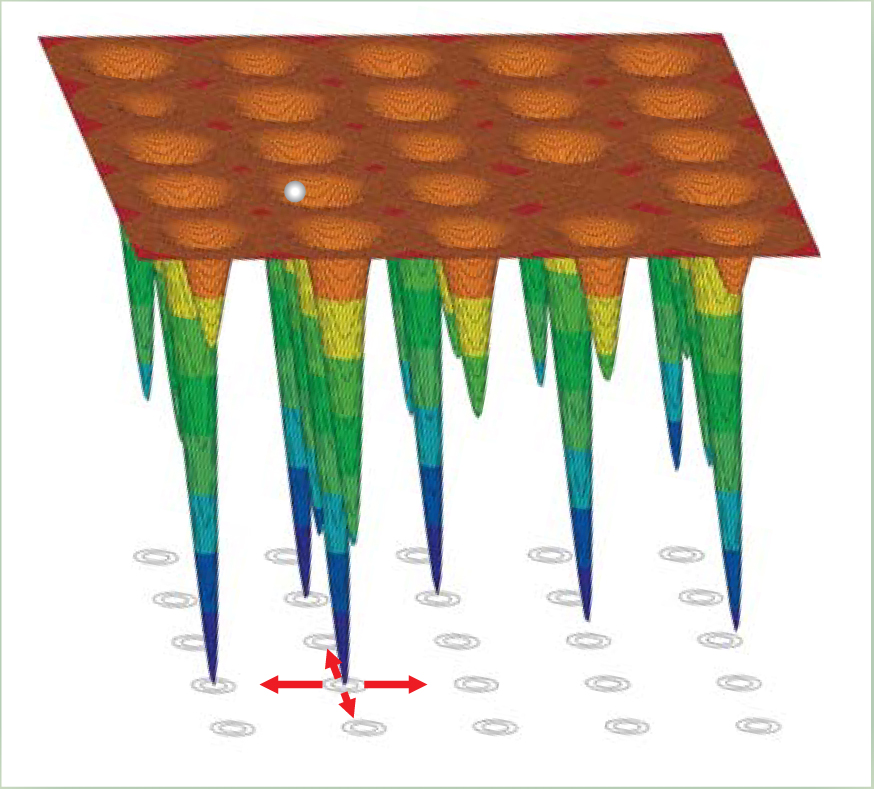
\includegraphics[width=0.9\textwidth]{hopping_picture_50years.jpg}}
\caption{Shematski prikaz Andersonovega modela v dveh dimenzijah. Slika je bila vzeta iz~\cite{lagendijk2009fifty}.  }
\label{fig:hopping_picture} 
\end{figure}
\begin{figure}[H]
\centering{
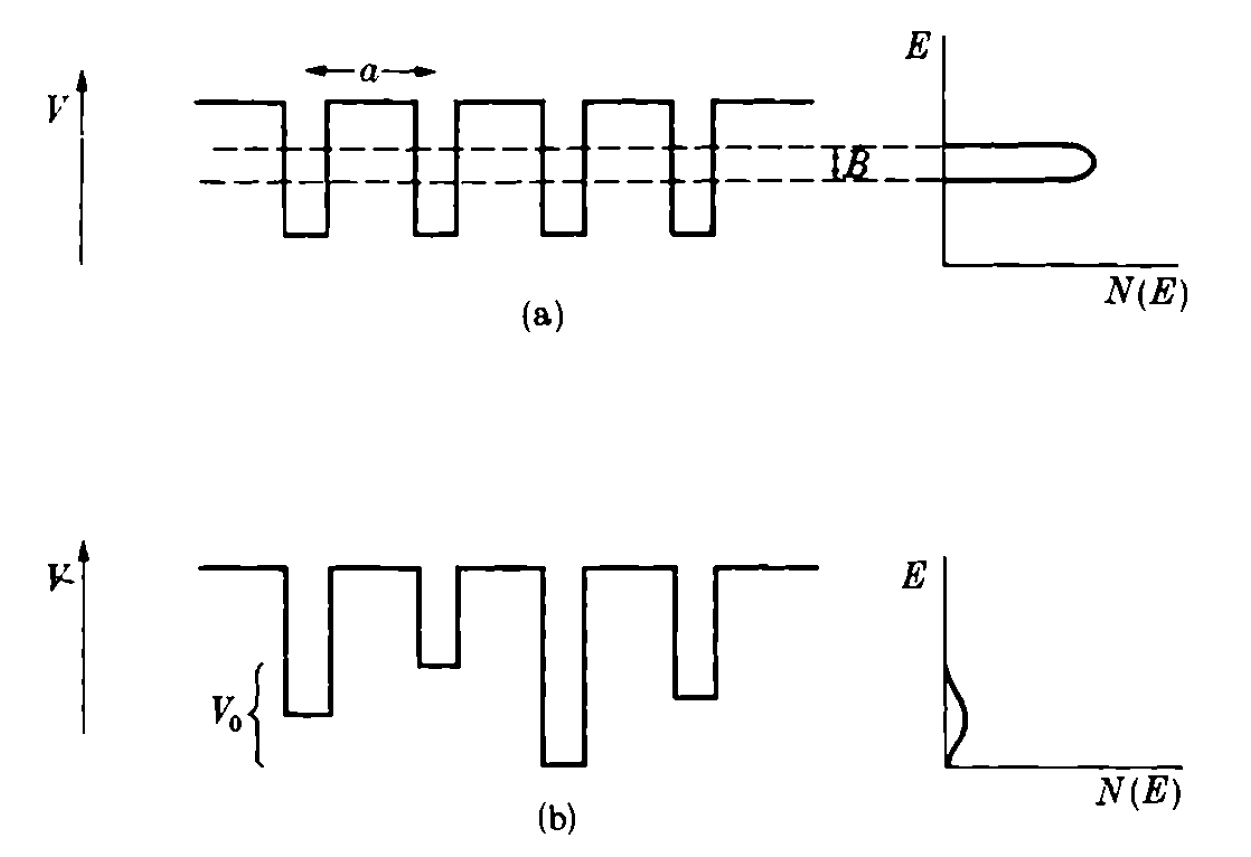
\includegraphics[width=1\textwidth]{bands.png}}
\caption{\textbf{a)} Shematski prikaz potencialnih jam za hamiltonko v približku tesne vezi ob odsotnosti nereda. \textbf{b)} Potencialne jame v Andersonovem modelu z naključnim potencialom. Na desni sta v obeh primerih shematsko prikazani gostoti stanj v treh dimenzijah. Uvedba nereda razširi pas in odpravi singularnosti gostote stanj. Slika je bila vzeta iz~\cite{mott2012electronic}.}
\label{fig:band_structure} 
\end{figure}
\end{minipage}{}
velikih fluktuacij naključnega potenciala. V prvem približku so energije tovrstnih enoelektronskih stanj določene kar z globinami naključnih potencialnih jam,
 zato se energije stanj z velikim prostorskim prekrivanjem tipično močno razlikujejo. Na drugi strani so stanja s podobnimi energijami v prostoru oddaljena in se le malo prekrivajo. Ker stanja ne v enem ne v drugem primeru ne morejo medsebojno hibridizirati, ostanejo v primeru dovolj močnega nereda lokalizirana. \\\\

% \begin{figure}[H]
% \floatbox[{\capbeside\thisfloatsetup{capbesideposition={left,center},capbesidewidth=5cm}}]{figure}[\FBwidth]
% {\caption{Shematski prikaz Andersonovega modela v dveh dimenzijah. Elektron lahko na urejeni kristalni mreži skače med sosednjimi mesti, ki imajo naključno porazdeljene potencialne energije. Slika je bila vzeta iz~\cite{lagendijk2009fifty}. }\label{fig:hopping_picture}}
% {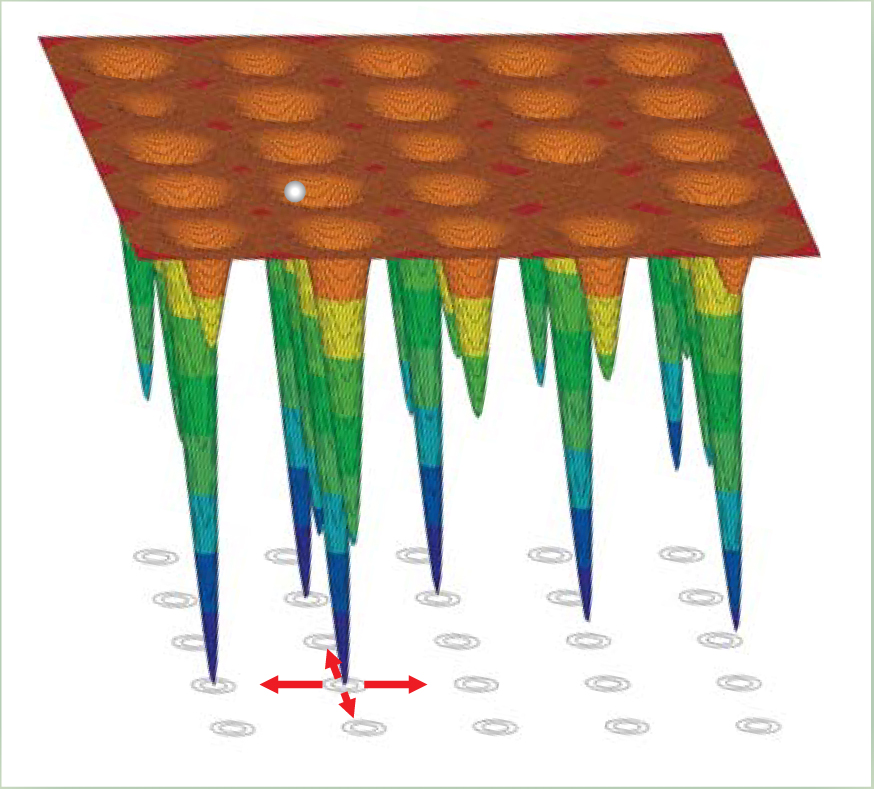
\includegraphics[width=0.4\textwidth]{hopping_picture_50years.jpg}}
% \end{figure} 
% \begin{minipage}[t]{0.5\textwidth}
% \noindent
% \textbf{Andersonov model}~\cite{anderson1958absence} je poseben primer modela, ki ga podaja En.~\eqref{eq:disc_ham}. Dobimo ga z upoštevanjem predpostavk izključno diagonalnega prispevka k neredu, skakanja elektronov zgolj med najbližjimi sosedi s konstantno hitrostjo tuneliranja $t$ in prisotnostjo le ene orbitale, $\nu=1$. Naključne potencialne energije $U_j$ so porazdeljene enakomerno na intervalu $\left[-W,W\right]$ v skladu s porazdelitvijo
% \begin{equation}\label{eq:and_prob}
% p(U_j)= \frac{1}{2W}\Theta \left(W - \abs{U_j} \right),
% \end{equation}
% kjer je $W$ \emph{parameter moči nereda}. Hamiltonka Andersonovega modela se tako zapiše kot 
% \begin{equation}\label{eq:Anderson_ham}
% H=\sum\limits_j U_j n_j + t\sum\limits_{\mathrm{n. s.}}\left(c^\dagger_i c_j + \mathrm{h.c.}\right),
% \end{equation}\\\\
% kjer je $n_j=c^\dagger_jc_j$ operator številske gostote delcev na $j$-tem mestu kristalne mreže.

% \end{minipage}\hfill
% \begin{minipage}[t]{0.47\textwidth}
% \begin{figure}[H]
% \centering{
% 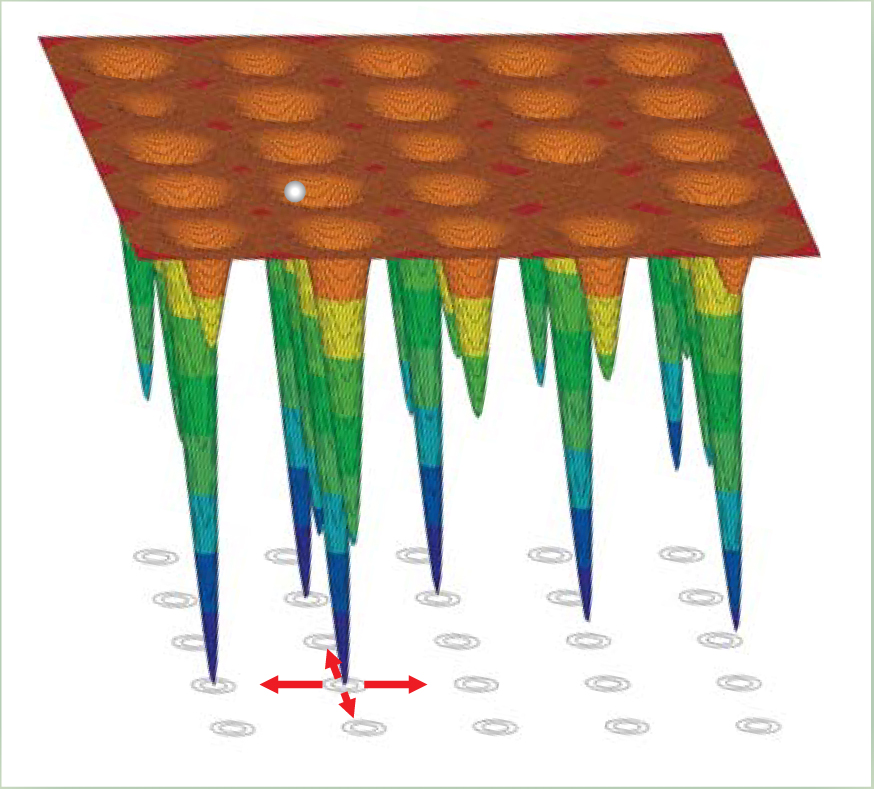
\includegraphics[width=0.65\textwidth]{hopping_picture_50years.jpg}}
% \caption{Shematski prikaz Andersonovega modela v dveh dimenzijah. Elektron lahko na urejeni kristalni mreži skače med sosednjimi mesti, ki imajo naključno porazdeljene potencialne energije. Slika je bila vzeta iz~\cite{lagendijk2009fifty}.  }
% \label{fig:hopping_picture} 
% \end{figure}
% \end{minipage}\\\\
\noindent 
\begin{minipage}[t]{0.56\textwidth} 

V treh dimenzijah za podkritične vrednosti nereda, $W<W_c$, v sistemu obstajajo tako lokalizirana kot razsežna stanja. V odsotnosti nereda so lastne funkcije Andersonove hamiltonke razsežna stanja Blochovega tipa. Uvedba majhnega nereda, ki ustreza majhnim vrednosti $W$, povzroči šibke naključne fluktuacije potenciala, ki vplivajo zgolj na stanja v bližini robov pasu, medtem ko ostanejo stanja v okolici sredine pasu bolj ali manj nespremenjena. Majhne fluktuacije potenciala namreč povzročijo nastanek plitkih \emph{naključnih} potencialnih jam, ki lahko lokalizirajo le nizkoenergijska lastna stanja hamiltonke. S povečevanjem parametra nereda amplituda potencialnih fluktuacij narašča, kar posledično vodi do lokalizacije stanj z višjo energijo. Lokalizirana in razsežna stanja ne morejo soobstajati pri istih energijah, 
\end{minipage}\hfill
\begin{minipage}[t]{0.42\textwidth} 
% \begin{figure}[H]
% \centering{
% 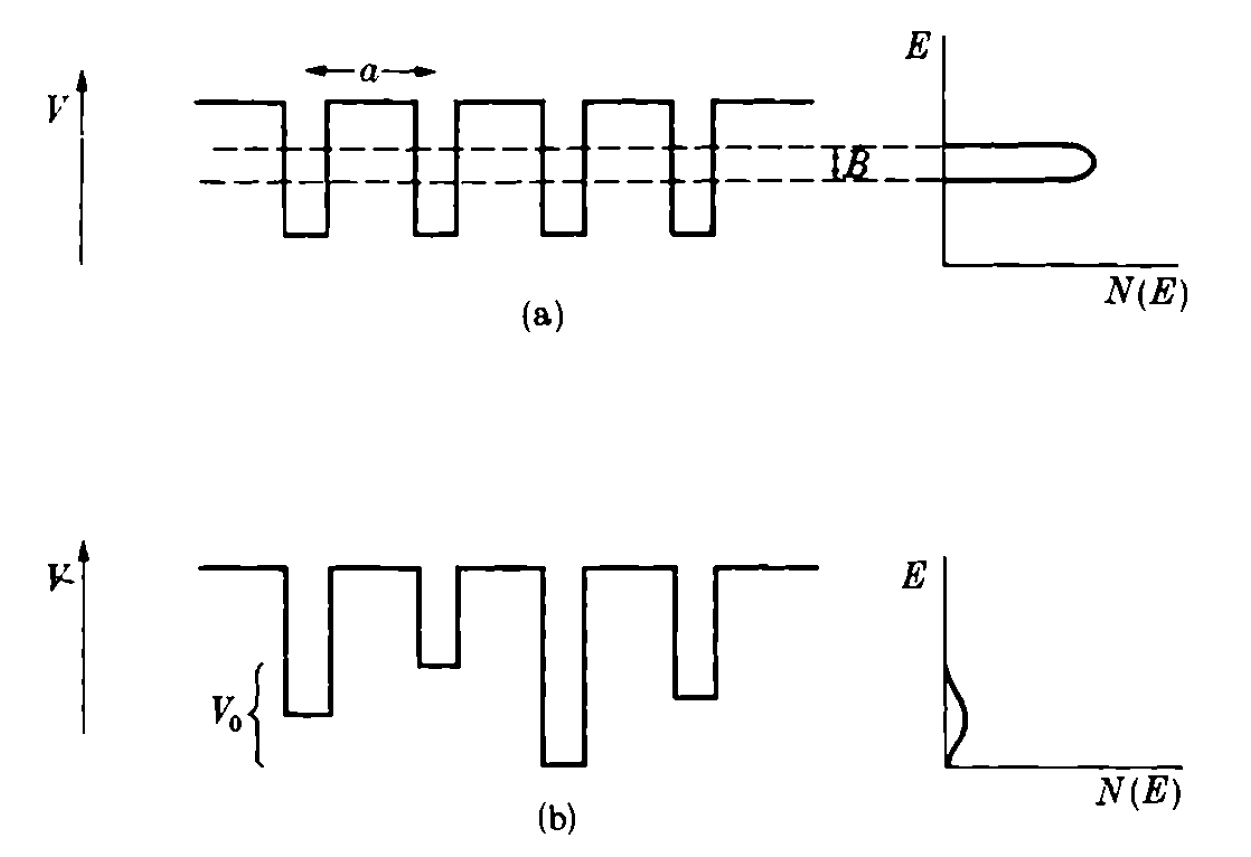
\includegraphics[width=1\textwidth]{bands.png}}
% \caption{\textbf{a)} Shematski prikaz potencialnih jam za hamiltonko v približku tesne vezi ob odsotnosti nereda. \textbf{b)} Potencialne jame v Andersonovem modelu z naključnim potencialom. Na desni sta v obeh primerih shematsko prikazani gostoti stanj v treh dimenzijah. Uvedba nereda razširi pas in odpravi singularnosti gostote stanj. Slika je bila vzeta iz~\cite{mott2012electronic}.}
% \label{fig:band_structure} 
% \end{figure}
\begin{figure}[H]
\centering{
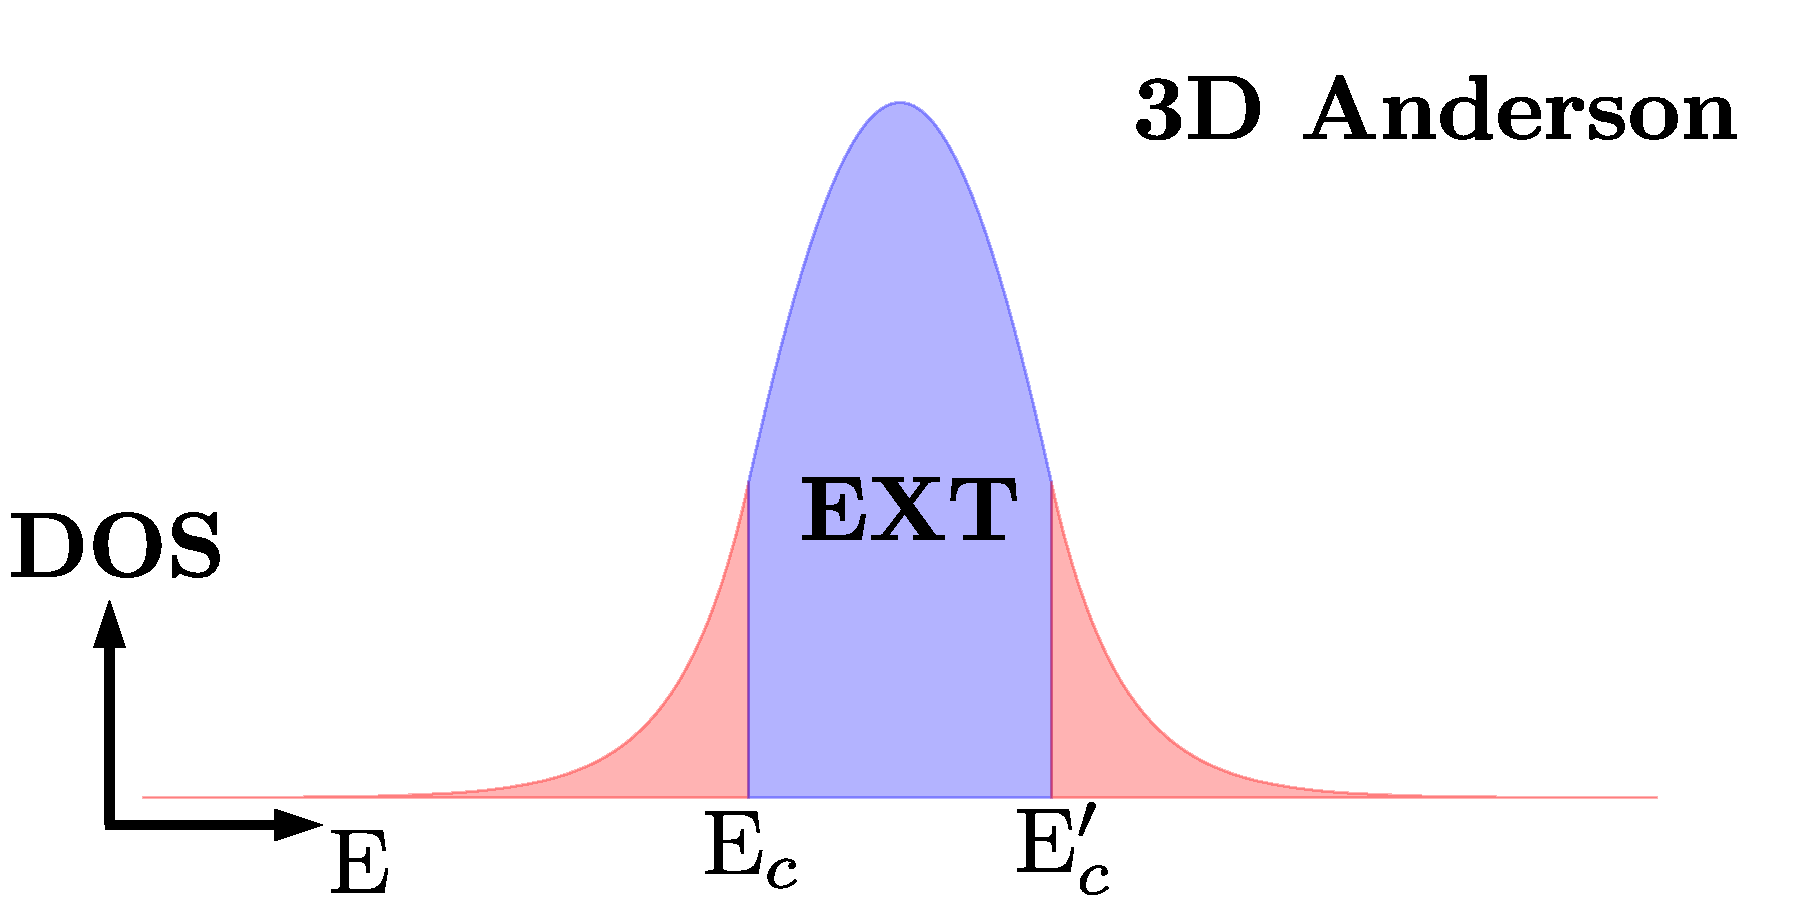
\includegraphics[width=0.95\textwidth]{mobility_edge_DOS_modified.pdf}}
\caption{Shematski prikaz tipične gostote stanj v odvisnosti od energije za tridimenzionalni Andersenov model za neko podkritično vrednost nereda, $W<W_c$. Stanja v robovih pasu (ki sta obarvana rdeče) so lokalizirana, medtem ko so stanja v sredini pasu (ki je obarvana modro) razsežna. $E_c$ in $E_c'$ označujeta roba mobilnosti, \textbf{EXT} pa razsežna stanja. }
\label{fig:mob_edge_DOS} 
\end{figure}
% \begin{figure}[H]
% \centering{
% 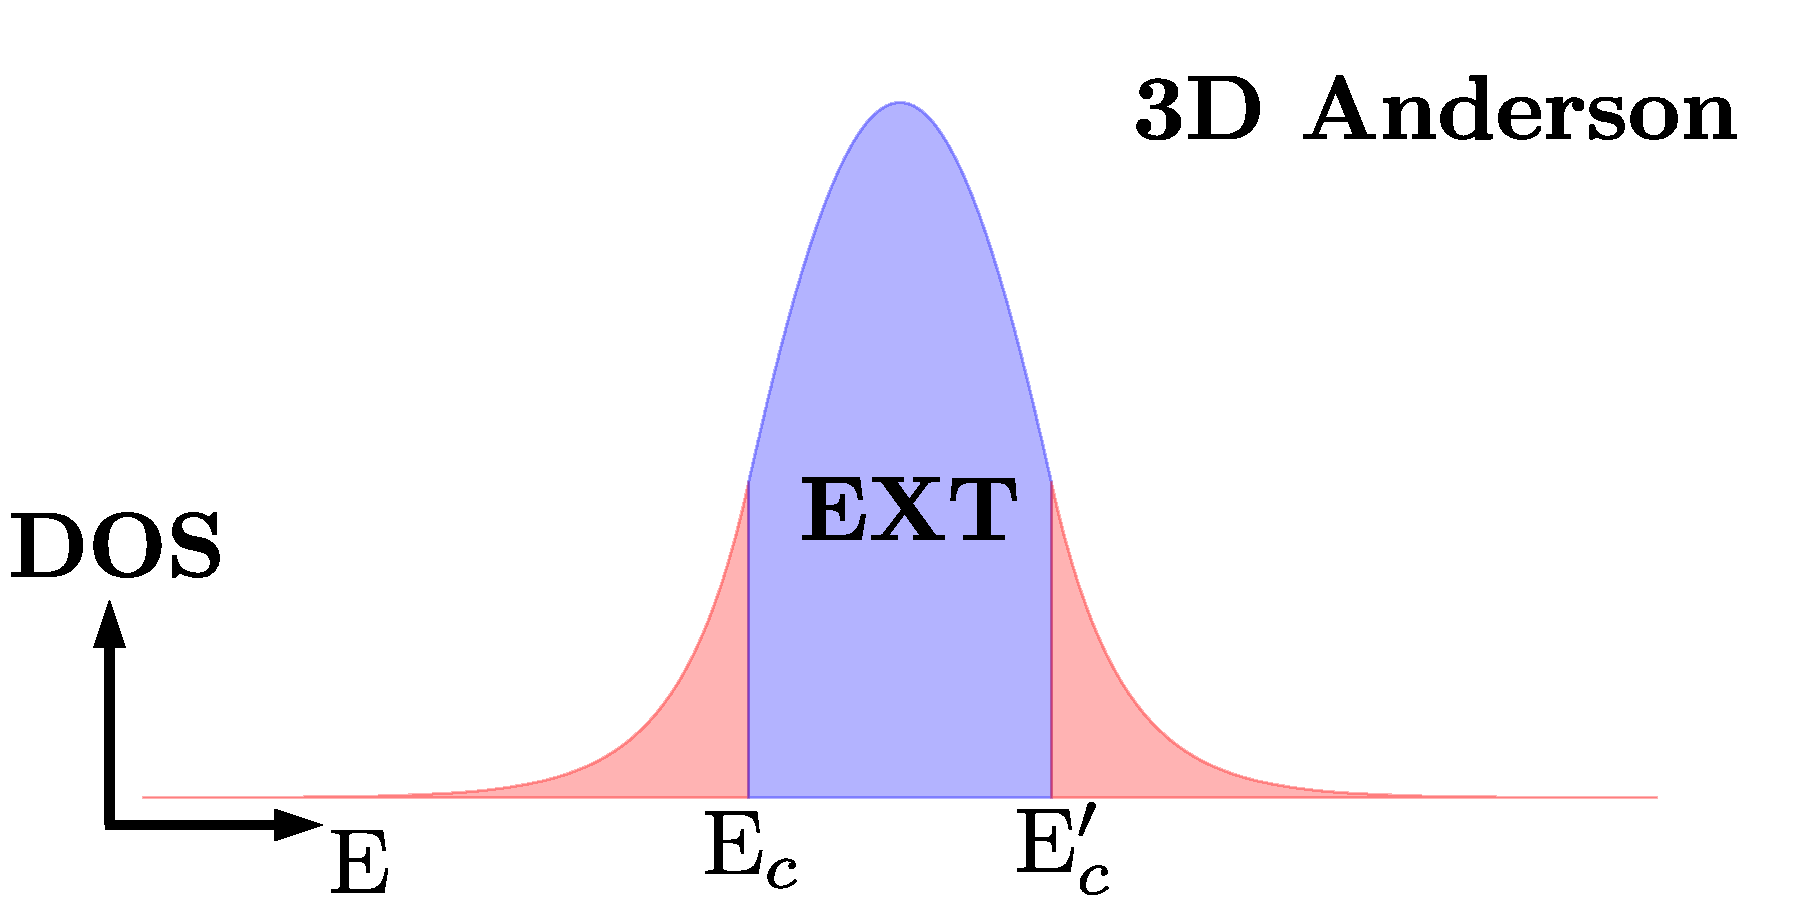
\includegraphics[width=0.95\textwidth]{mobility_edge_DOS_modified.pdf}}
% \caption{A schematic of a typical density of states (DOS) distribution with respect to energy for a three-dimensional Anderson model for some intermediate disorder $W<W_c$. States in the band tails (coloured red) are localized while those in the middle (coloured blue) are extended. }
% \label{fig:DOS} 
% \end{figure}
\end{minipage}
saj bi v tem primeru lokalizirana stanja zaradi znatnega prekrivalnega integrala in ujemajočih se energij z razsežnimi stanji tvorila hibridizirana stanja in tako postala razsežna.
 Energije lokaliziranih in razsežnih stanj v splošnem loči kritična energija $E_c$ oziroma rob mobilnosti. Ker je Andersonova hamiltonka simetrična na zamenjavo delcev in vrzeli ima Andersonov model kar dva mobilnostna roba $E_c$ in $E_c'$. Kot prikazuje Slika~\ref{fig:mob_edge_DOS}, nastopata simetrično glede na središče pasu, ki se mu približujeta z naraščanjem parametra $W$. Polna lokalizacija vseh valovnih funkcij nastopi, ko se mobilnostna roba združita, saj tedaj v sistemu ni več razsežnih stanj. To se zgodi pri kritični vrednosti parametra nereda $W_c$. V primeru obstoja roba mobilnosti je sistem pri ničelni temperaturi izolator, če je njegova Fermijeva energija $\varepsilon_\mathrm{F}$ znotraj energijskega območja lokaliziranih stanj. V tem primeru je pri končnih temperaturah specifična prevodnost končna in sorazmerna eksponentno majhnemu številu zasedenih razsežnih stanj,
\begin{equation}
\sigma(T)\propto \exp\left(\frac{\varepsilon_1 - \varepsilon_\mathrm{F}}{T}\right).
\end{equation}
Pri tem je $\varepsilon_1$ energija celotnega sistema, torej vsota enodelčnih energij.  \\\\
Na Sliki~\ref{fig:light_cone} je za enodimenzionalni Andersonov model prikazana razlika med odsotnostjo nereda in močnim neredom v primeru unitarnega časovnega razvoja začetnega profila verjetnostne gostote. Na verigi dolžine $L=1000$ je bilo pripravljeno začetno stanje z enotsko verjetnostno gostoto le na mestu v sredini verige, medtem ko je bila gostota povsod drugod ničelna. V odsotnosti nereda se je začetni profil sčasoma balistično razširil, tako da je bila po dolgem času verjetnostna gostota po celem sistemu enakomerna. Nasprotno je v prisotnosti močnega nereda verjetnostna gostota vselej ostala lokalizirana v okolici sredine verige. \newpage
% \begin{figure}[H]
% \floatbox[{\capbeside\thisfloatsetup{capbesideposition={left,center},capbesidewidth=3cm}}]{figure}[\FBwidth]
% {\caption{Primer časovnega razvoja začetnega stanja v primeru brez nereda in z močnim neredom ($W=3.0$). Pri tem $t$ označuje čas, $j$ pa mesto v enodimenzionalni verigi. Za medmrežno razdaljo smo privzeli $a=1$, enako tudi za enoto časa.  }\label{fig:light_cone}}
% {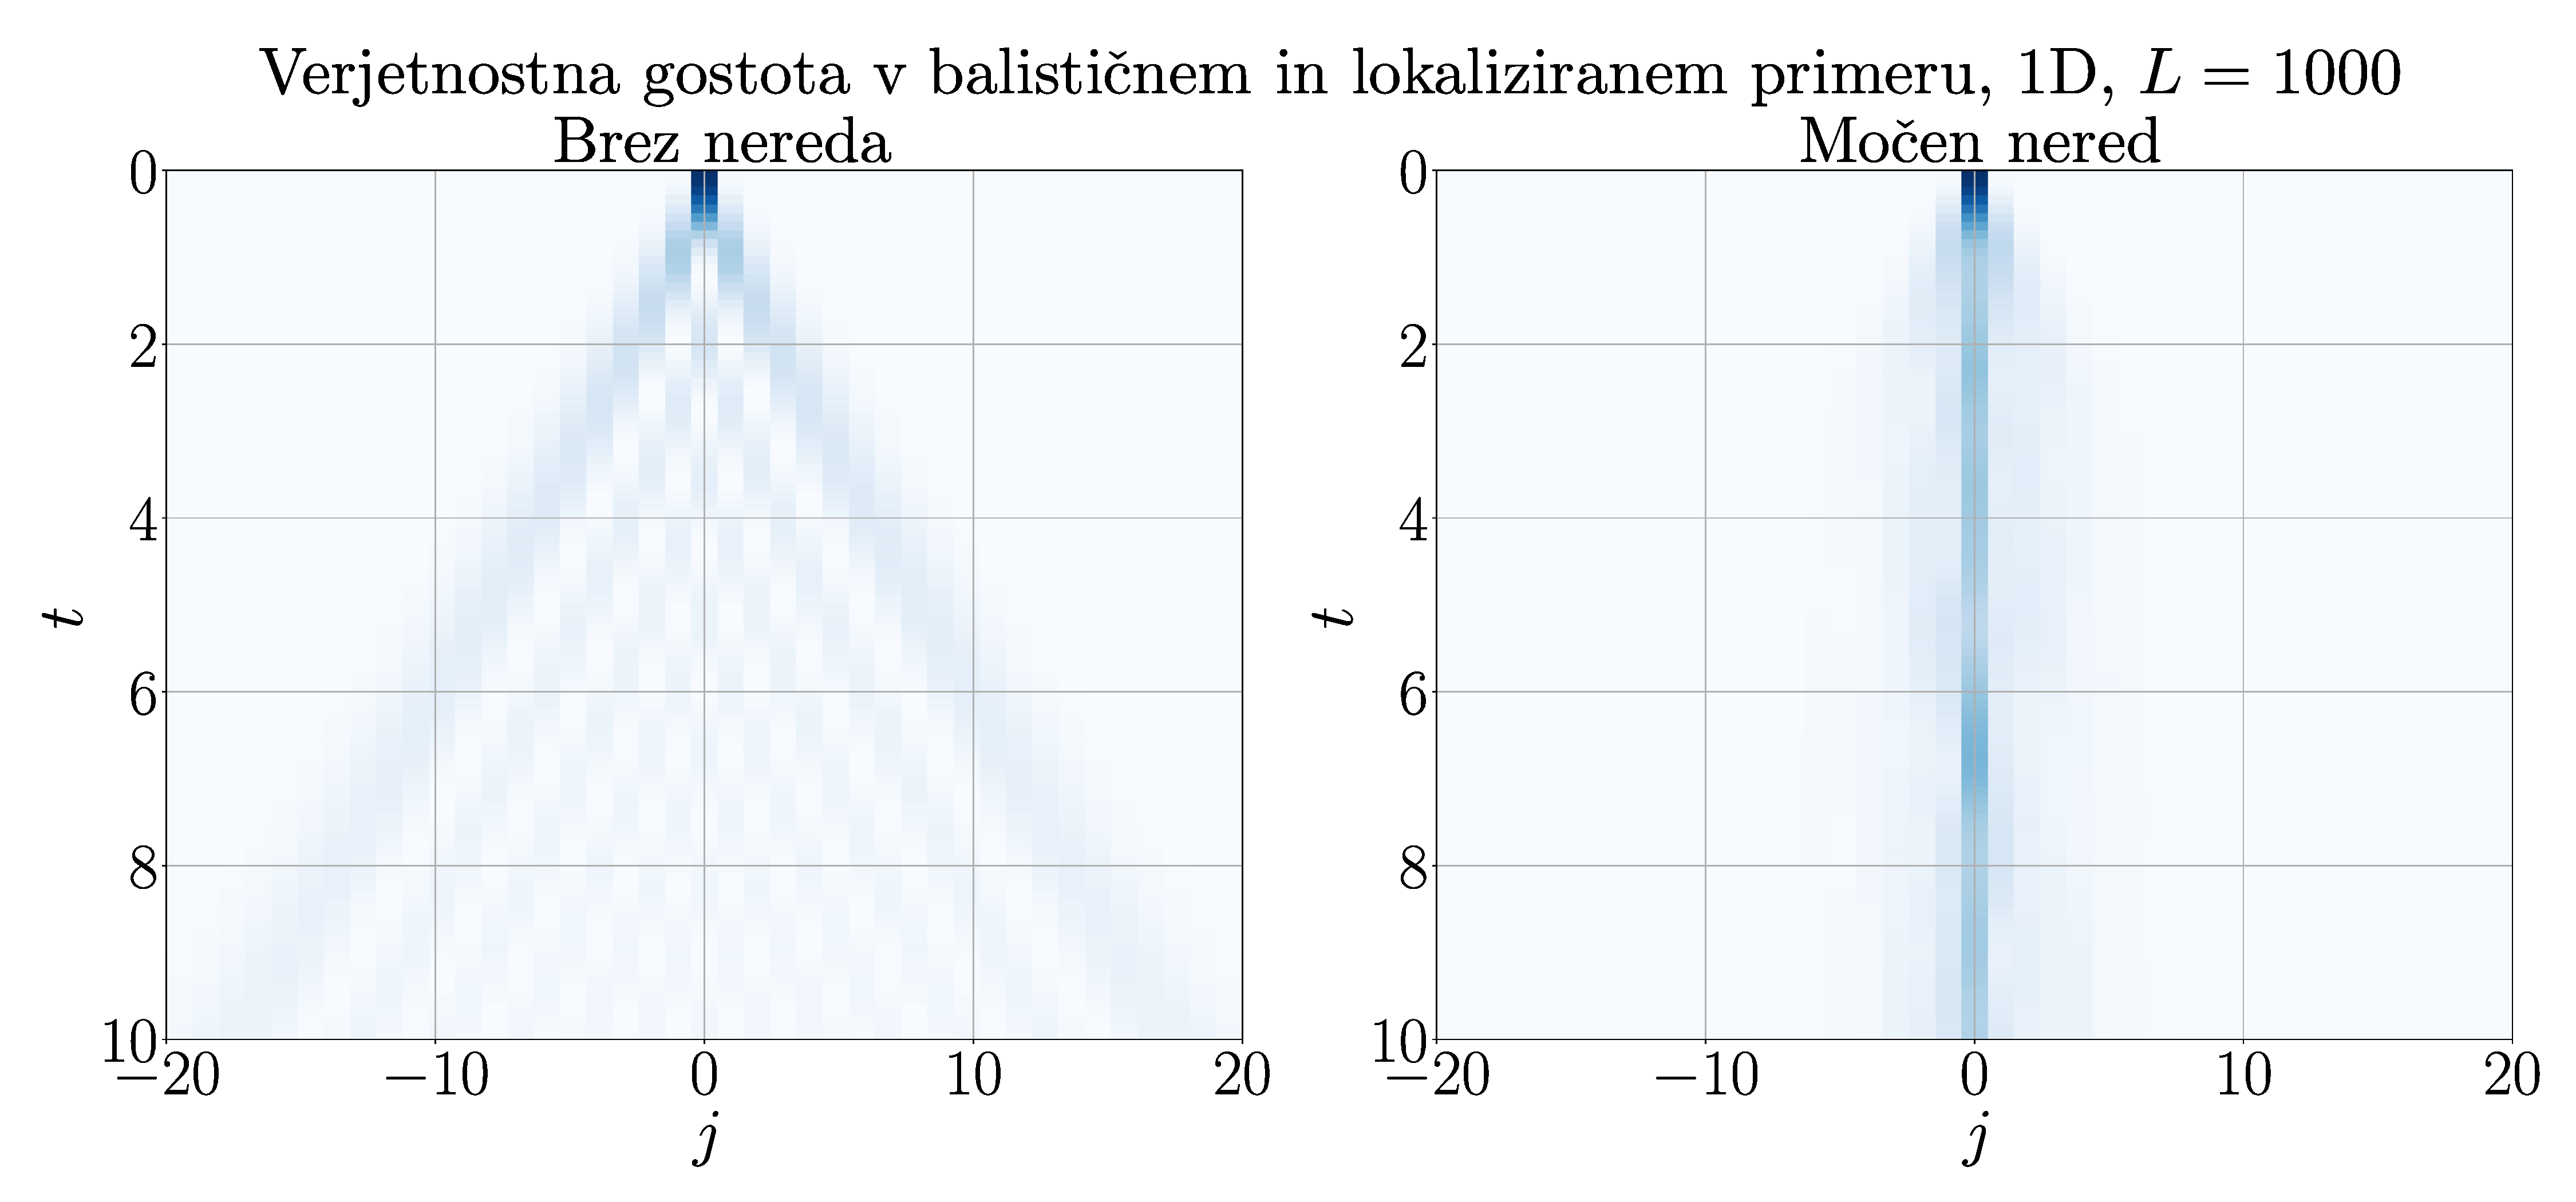
\includegraphics[width=0.85\textwidth]{1D_Anderson_localization_Seminar_scaling_analysis_D1_shape_1000_light_cone_double_presentation.pdf}}
% \end{figure} 
\begin{figure}[H]
\centering{
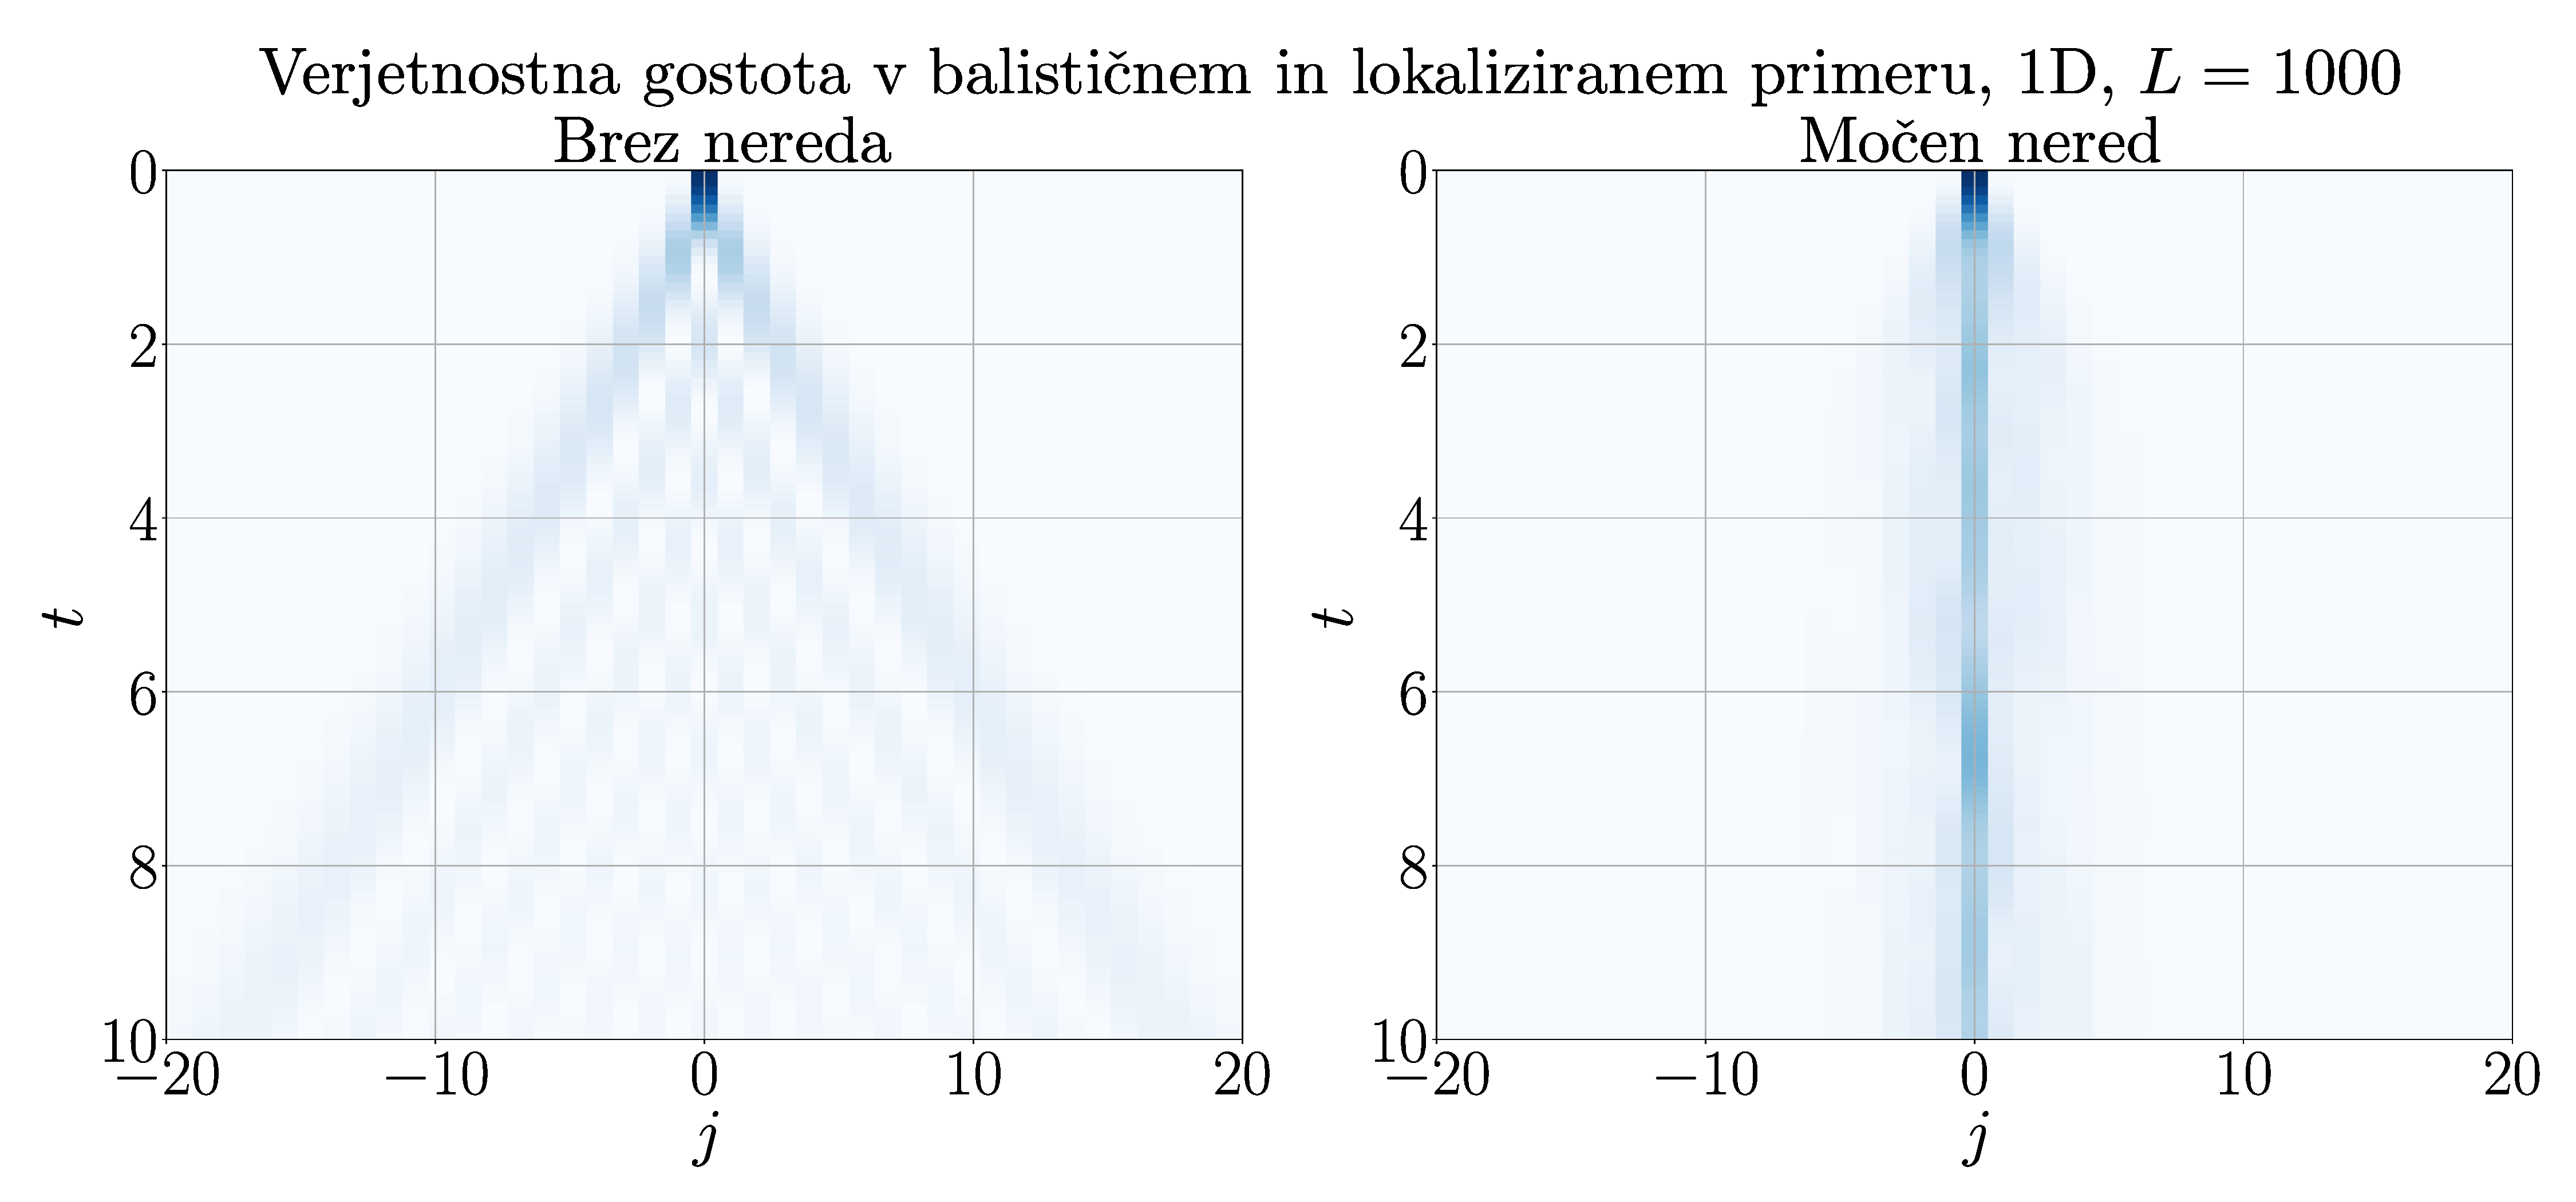
\includegraphics[width=0.95\textwidth]{1D_Anderson_localization_Seminar_scaling_analysis_D1_shape_1000_light_cone_double_presentation.pdf}}
\caption{Primer časovnega razvoja začetnega stanja v primeru brez nereda in z močnim neredom ($W=3.0$). Pri tem $t$ označuje čas, $j$ pa mesto v enodimenzionalni verigi. Za medmrežno razdaljo smo privzeli $a=1$, enako tudi za enoto časa. }
\label{fig:light_cone} 
\end{figure}
\section{Lokalizacija v sistemih z meddelčnimi interakcijami}
\label{lokalizacija_v_sistemih_z_med}
Do sedaj smo se ukvarjali z lokalizacijo v sistemih neinteragirajočih delcev. Pri opisu dejanskih sistemov predstavlja predpostavka odsotnosti meddelčnih interakcij glavno pomanjkljivost modelov enodelčne lokalizacije. V praksi so namreč interakcije vselej prisotne, njihov vpliv pa vse od Andersonovega prelomnega članka ostaja eno pomembnejših odprtih vprašanj področja. Polno lokaliziran Andersonov izolator brez roba mobilnosti namreč pri nobeni temperaturi ne omogoča transporta energije ali naboja in tako zaradi ničelne prevodnosti vselej preprečuje termalizacijo. Da bi v interagirajočih sistemih lahko z gotovostjo potrdili oziroma ovrgli odsotnost termalizacije in nastop večdelčne lokalizacije, moramo v dosedanjo obravnavo neinteragirajočih sistemov neizogibno vključiti meddelčne interakcije in preučiti njihov vpliv. Zavoljo pregleda nad raziskovalno dejavnostjo in za lažjo umestitev v časovni okvir je na tem mestu navedenih nekaj zgodovinsko pomembnejših del s področja, v katerih je bil obravnavan preplet interakcij in nereda. Pri tem sledimo Ref.~\cite{abanin2018ergodicity}.\\\\
Leta 1980 sta Fleishman in Anderson~\cite{fleishman1980interactions} podala kvalitativne argumente v prid nastopu lokalizacije ob prisotnosti šibkih interakcij kratkega dosega. Uporaba teorije renormalizacijske grupe je omogočila posplošitev koncepta Andersonovega izolatorja in posledično opis osnovnih stanj neurejenih sistemov z interakcijami. V ta okvir spada delo Finkelsteina~\cite{finkelshtein1983influence}, ki je leta 1983 pri nadgraditvi skalirne teorije lokalizacije upošteval preplet vpliva meddelčnih interakcij in nereda. Mnogo kasneje so se pojavile utemeljitve obstoja lokalizirane faze ob prisotnosti interakcij pri \emph{končnih} temperaturah. Med prvimi so na to možnost leta 1997 pokazali Altshuler in sodelavci~\cite{altshuler1997quasiparticle} na primeru ničdimenzionalne kvantne pike. Obstoj lokalizacije v višjedimenzionalnih sistemih z lokalnimi interakcijami so leta 2006 utemeljili Basko, Aleiner in Altshuler~\cite{basko2006metal}, in sicer za nizke temperature oziroma nizke energijske gostote. V Ref.~\cite{basko2006metal} uporabljeni modelski sistem je namreč idealen izolator z ničelno prevodnostjo pri nizkih energijskih gostotah, medtem ko postanejo večdelčna lastna stanja pri visokih energijskih gostotah delokalizirana. To označuje fazni prehod med izolatorsko in prevodno fazo, ki nastopi pri končni temperaturi, oziroma točneje, pri končni energijski gostoti nad osnovnim stanjem, poimenovani \emph{večdelčni rob mobilnosti}. Fazni prehod v večdelčno lokalizirano stanje je kvalitativno drugačen od konvencionalnih končnotemperaturnih prehodov med kovino in izolatorjem v Mottovih in pasovnih izolatorjih. V slednjih je namreč specifična prevodnost pri končni temperaturi končna, vendar eksponentno majhna, medtem ko je v nizkotemperaturnem režimu večdelčno lokalizirane faze \emph{identično} enaka nič~\cite{basko2006problem}. Obstoj večdelčno lokalizirane faze tudi pri neskončni temperaturi v neurejenem interagirajočem sistemu na diskretni mreži sta leta 2007 utemeljila Oganesyan in Huse~\cite{PhysRevB.75.155111}, in sicer na podlagi numerične analize enodimenzionalnega modela s fermioni brez spinskih prostostnih stopenj. Z uporabo polne diagonalizacije modelskih hamiltonk in študijo spektralnih statistik sta prišla do rezultatov, ki napovedujejo obstoj večdelčno lokalizirane faze v neurejenih modelih na diskretnih mrežah tudi ob neskončnih temperaturah oziroma pri energijskih gostotah visoko nad osnovnim stanjem. Napoved velja za sisteme s končnodimenzionalnimi lokalnimi Hilbertovimi prostori, torej sisteme s končnim številom stanj na mesto. 
Članek je navdahnil številne kasnejše numerične raziskave MBL pojavov, po njem pa se pri analizi spektralnih statistik v magistrski nalogi obravnavanih modelov zgledujemo tudi mi.
\\\\ 
Čeprav koncepti v podpoglavju~\ref{anderson} obravnavane Andersonove lokalizacije služijo kot izhodišče za obravnavo fenomenov večdelčne lokalizacije, se problema bistveno razlikujeta, zato vključitev meddelčnih interakcij terja razvoj novih pristopov.
 % Interakcije v interagirajočih večdelčnih sistemih sklapljajo različna večdelčna stanja. V kolikor v sistemu obstajajo delokalizirana stanja, lahko interakcije denimo omogočijo prehod iz lokaliziranega osnovnega stanja v vzbujeno delokalizirano večdelčno stanje in povzročijo fazni prehod med izolatorskim in prevodnim obnašanjem. 
 Pri presoji obstoja večdelčno lokalizirane faze moramo preučiti naravo vseh večdelčnih lastnih stanj sistema in ugotoviti, ali so lokalizirana ali ne. Ker preučujemo stanja s končnimi energijskimi gostotami nad energijo osnovnega stanja, nas zanimajo končne temperature. Na drugi strani so bili zaradi odsotnosti meddelčnih interakcij pri Andersonovem izolatorju v večini študij preučevani le osnovno stanje in končno število vzbuditev nad njim. V termodinamski limiti neskončnega sistema je energijska gostota vzbuditev enaka nič, kar ustreza ničelni temperaturi. 
\\\\
V nadaljevanju razložimo osnovne koncepte fizike zaprtih kvantnih sistemov. Ker je poglavitna lastnost MBL sistemov odsotnost termalizacije, je zatem podrobneje predstavljen mehanizem termalizacije v kvantnih sistemih skupaj s hipotezo termalizacije lastnih stanj (v nadaljevanju ETH). Nazadnje so navedene najpomembnejše značilnosti MBL sistemov. 
\subsection{Fizika zaprtih kvantnih sistemov}
\begin{minipage}[t]{0.4\textwidth}
\noindent \\\\
Pojav MBL se tipično preučuje v zaprtih kvantnih sistemih, kjer zaprtost pomeni odsotnost sklopitve z okolico oziroma zunanjim rezervoarjem, kot prikazuje Slika~\ref{fig:nandkishore_huse_reservoir}. V tem podpoglavju navedemo osnovne koncepte, ki določajo obnašanje tovrstnih sistemov. V razpravi imamo vselej v mislih časovno neodvisne hamiltonke z interakcijami kratkega dosega. \\\\
\end{minipage}\hfill
\begin{minipage}[t]{0.55\textwidth}
\begin{figure}[H]
\centering{
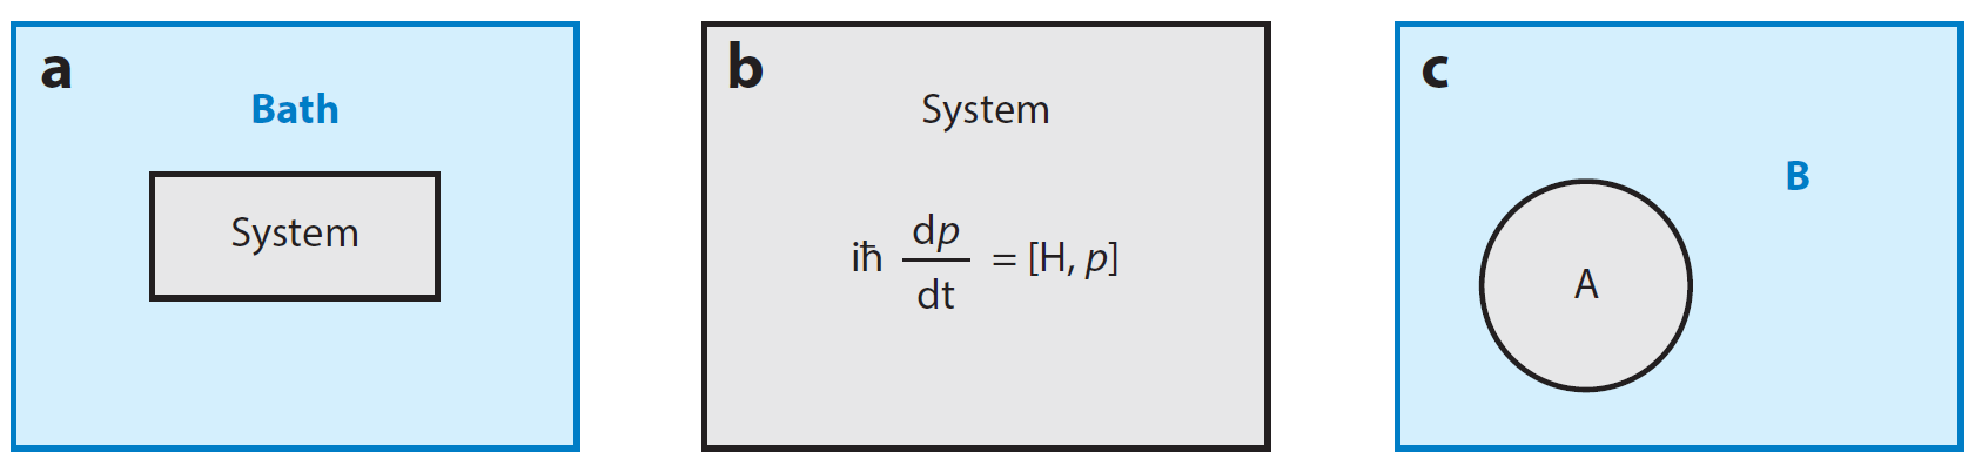
\includegraphics[trim=0 0 340 0,clip, width=0.87\textwidth]{nandkishore_huse_reservoir.pdf}}
\caption{
\textbf{a)} Pri običajnem kvantnostatističnem opisu sistema privzamemo njegovo sklopitev z zunanjim rezervoarjem, s katerim lahko izmenjuje denimo energijo in delce. \textbf{b)} Tu obravnavamo zaprte oziroma izolirane kvantne sisteme, katerih dinamiko določa unitaren časovni razvoj začetnih stanj. 
% \textbf{c)} Pri obravnavi termalizacije v zaprtih kvantnih sistemih je smiselno sistem razdeliti na podsistema A in B, pri čemer je v A makroskopsko zanemarljiv delež prostostnih stopenj celotnega sistema. V kolikor večji podsistem B manjšemu podsistemu služi kot toplotni rezervoar, je termalizacija možna tudi v zaprtem kvantnem sistemu. 
Slika je bila vzeta iz Ref.~\cite{nandkishore2015many}. 
}
\label{fig:nandkishore_huse_reservoir}
\end{figure}
\end{minipage}
Poljubno stanje zaprtega kvantnega sistema ob času $t$ opisuje gostotna matrika, $\rho(t)=\ket{\psi(t)}\bra{\psi(t)}$. 
V Schrödingerjevi sliki, kjer je časovni razvoj poljubnega začetnega 
 stanja določen z delovanjem unitarnega časovnega propagatorja, 
\begin{equation}\label{eq:cas_razvoj}
\ket{\psi(t)}=\mathrm{e}^{-\iu H t/\hbar}\ket{\psi(0)},
\end{equation}
 je časovni razvoj gostotne matrike določen z zvezami 	
% Pojav MBL se tipično preučuje v zaprtih kvantnih sistemih, kjer zaprtost pomeni odsotnost sklopitve z okolico oziroma zunanjim rezervoarjem. V tem podpoglavju navedemo osnovne koncepte, ki določajo obnašanje tovrstnih sistemov. V razpravi imamo vselej v mislih časovno neodvisne hamiltonke z interakcijami kratkega dosega. 
% \paragraph{Unitaren časovni razvoj kvantnih sistemov}
% Ker se pri obravnavi ne omejujemo izključno na čista stanja, opisuje poljubno stanje zaprtega kvantnega sistema gostotna matrika, $\hat{\rho}(t)=\ket{\psi(t)}\bra{\psi(t)}$. V Schrödingerjevi sliki, kjer je časovni razvoj poljubnega začetnega stanja določen z delovanjem unitarnega časovnega propagatorja, 
% \begin{equation}\label{eq:cas_razvoj}
% \ket{\psi(t)}=\mathrm{e}^{-\iu H t}\ket{\psi(0)},
% \end{equation}
%  je časovni razvoj gostotne matrike določen z zvezami 	
\begin{equation}\label{eq:cas_razvoj_matrike}
\rho(t)=\mathrm{e}^{-\iu H t}\rho(0)\ \mathrm{e}^{\iu H t}, \hspace{5mm} \iu\frac{\dd \rho}{\dd t}=\left[H, \rho\right]; \hspace{5mm} \Tr{\rho}=1.
\end{equation}
Na vmesnem koraku med En.~\eqref{eq:cas_razvoj} in \eqref{eq:cas_razvoj_matrike} smo postavili $\hbar=1.$ Vsi drugi kvantnomehanski operatorji $\hat{O}$ so časovno neodvisni, pričakovana vrednost poljubnemu operatorju $\hat{O}$ pripadajoče opazljivke $O$ pa se ob času $t$ zapiše kot 
\begin{equation}
\langle \hat{O}\rangle_t = \Tr\left(\hat{O}\hat{\rho}(t)\right).
\end{equation}
V klasični statistični mehaniki temelji koncept termalizacije na predpostavki \emph{ergodičnosti}, v skladu s katero so na dolgem časovnem intervalu vsa mikrostanja sistema obiskana z enako verjetnostjo. Zaradi linearnosti kvantne mehanike moramo v kvantnih sistemih pojem ergodičnosti nekoliko prilagoditi. Vzemimo namreč poljubno začetno neravnovesno stanje večdelčnega sistema $\ket{\psi(0)}$ in ga razvijmo po bazi večdelčnih lastnih stanj hamiltonke $H$, ki določa dinamiko sistema:
\begin{equation}\label{eq:lastna_stanja}
\ket{\psi(0)}=\sum\limits_\alpha A_\alpha \ket{\alpha}, \hspace{5mm} H\ket{\alpha}=E_\alpha\ket{\alpha}.
\end{equation}
 Pri časovnem razvoju v skladu z En.~\eqref{eq:cas_razvoj} pridobi vsak izmed koeficientov razvoja $A_\alpha$ multiplikativni fazni faktor, ki ustreza dani večdelčni lastni energiji $E_\alpha$, 
$$
\ket{\psi(t)}=\mathrm{e}^{-\iu H t}\ket{\psi(0)}=\sum\limits_\alpha A_\alpha \mathrm{e}^{-\iu E_\alpha t}\ket{\alpha}.
$$
Verjetnost $p_\alpha$, da se sistem nahaja v enem izmed lastnih stanj $\ket{\alpha}$, se s časom seveda ne spreminja in je določena z začetno izbiro stanja, saj velja $p_\alpha=\abs{A_\alpha}^2$. To je popolnoma drugače kot v klasičnih sistemih, ki med časovnim razvojem obiščejo različne dele faznega prostora. V kvantnih sistemih je pojem termalizacije namesto s samimi valovnimi funkcijami	ali gostotnimi matrikami smiselno povezati  s pričakovanimi vrednostmi \emph{lokalnih} opazljivk po dolgem času, ki jih podaja izraz~\cite{deutsch1991quantum}~\cite{abanin2018ergodicity}
\begin{equation}\label{eq:ergodicnost_kvantno}
\begin{split}
\langle \hat{O}\rangle_\infty &=\lim_{t'\to\infty}\frac{1}{t'}\int\limits_0^{t'} \bra{\psi(t)}\hat{O}\ket{\psi(t)}\dd t =\\
&=\lim_{t'\to\infty}\frac{1}{t'}\int\limits_0^{t'}\left\{\sum\limits_\alpha\abs{A_\alpha}^2\bra{\alpha}\hat{O}\ket{\alpha}+        \sum\limits_{\alpha\neq\beta} A_\alpha^* A_\beta\mathrm{e}^{\iu\left(E_\alpha-E_\beta\right)t} \bra{\alpha}\hat{O}\ket{\beta}\right\}\dd t=\\
 &=\sum\limits_\alpha p_\alpha\bra{\alpha}\hat{O}\ket{\alpha}.
 \end{split}
\end{equation}
Iz En.~\eqref{eq:ergodicnost_kvantno} vidimo, da vrednost $\langle \hat{O}\rangle_\infty$ določajo verjetnosti $p_\alpha$ skupaj s pričakovanimi vrednostmi opazljivke $\bra{\alpha}\hat{O}\ket{\alpha}$. Izvendiagonalni matrični elementi v zgornji enačbi namreč oscilirajo pri različnih frekvencah in se pri časovni integraciji v procesu \emph{izgube faze} (ang.~\emph{dephasing}) izpovprečijo, pri čemer smo privzeli nedegeneriranost lastnih stanj $\ket{\alpha}.$ 
\\\\
Pri eksperimentih in numeričnih simulacijah je limita neskončnega časa v zgornji enačbi seveda nedosegljiva. Numerične študije kažejo, da mora biti $t'$ daljši od tipičnega relaksacijskega časa sistema. Ker je določitev relaksacijskih časov specifična od modela do modela, gre za eno izmed odprtih vprašanj s področja. Podrobnejša obravnava najprimernejše dolžine integracijskega intervala zato presega okvire magistrske naloge. 
% V praksi mora biti integracijski čas $t'$ daljši vsaj od Heisenbergovega časa~\cite{srednicki1999approach}, $\tau_\mathrm{H}\equiv 2\pi/\delta.$ Pri tem je $\delta$ povprečen razmik med energijskimi nivoji v hamiltonki $H.$ Ker gre za eno izmed odprtih vprašanj s področja, podrobnejša obravnava najprimernejše dolžine integracijskega intervala presega okvire magistrske naloge.
\\\\
V generičnih sistemih fluktuacije okrog povprečne vrednosti $\langle\hat{O}\rangle_\infty$ z velikostjo sistema padajo eksponentno, njihovo časovno odvisnost pa določajo izvendiagonalni matrični elementi v En.~\eqref{eq:ergodicnost_kvantno}. Čeprav so slednji pomembni tudi v hipotezi termalizacije lastnih stanj, ki je predstavljena v nadaljevanju, za nas niso bistveni. Zanimajo nas namreč le ravnovesne vrednosti opazljivk, medtem ko tudi natančnejša obravnava časovne dinamike relaksacije proti ravnovesnim vrednostim presega okvire magistrske naloge. 
  


% Medtem ko enačba~\eqref{eq:ergodicnost_kvantno} podaja pričakovano vrednost opazljivke $\hat{O}$ po dolgem času, ne pove nič o časovni odvisnosti fluktuacij okrog $\langle\hat{O}\rangle_\infty.$
% \\\\
%  Te z naraščanjem sistema tipično padajo proti ničelni vrednosti, pri čemer je za generične sisteme padanje eksponentno z velikostjo sistema. Natančnejša obravnava časovnih fluktuacij pričakovanih vrednosti opazljivk presega okvire te magistrske naloge. Limita neskončnega časa v En.~\eqref{eq:ergodicnost_kvantno} je v eksperimentih in numeričnih simulacijah seveda nedosegljiva. V praksi mora biti 

% Pri tem moramo dodati, da zaradi posledic efektov končnih velikosti sistemov $\langle\hat{O}\rangle_\infty$ doseže ravnovesno vrednost samo v termodinamski limiti neskončnega sistema, kjer moramo v En.~\eqref{eq:ergodicnost_kvantno} limito neskončnega sistema izvesti hkrati z limito $t\to\infty.$  Za končne sisteme je časovna dinamika namreč kvaziperiodična in tako dolgočasovna limita ni dobro definirana, medtem ko po končnem času difuzivna propagacija v termalizirajočem sistemu doseže le končen delež neskončnega sistema~\cite{PhysRevB.75.155111}. 

% \subsubsection{Termalizacija v zaprtih kvantnih sistemih}
% Intuitivno si lahko mislimo, da zaprt kvantni sistem termalizira, če se za fizikalno začetno stanje po dovolj dolgem času pričakovane vrednosti opazljivk, dane z En.~\eqref{eq:ergodicnost_kvantno}, ujemajo z ustreznimi ansambelskimi povprečji - v limiti neskončnega sistema dobimo v mikrokanoničnem, kanoničnem in velekanoničnem ansamblu enake rezultate. S fizikalnimi stanji mislimo na eksperimentalno dosegljiva stanja, kot so denimo produktna stanja ali superpozicije ekstenzivno mnogo lastnih funkcij, medtem ko posamezne lastne funkcije ne predstavljajo fizikalnih stanj. Čas, potreben za njihovo pripravo namreč skalira eksponentno z velikostjo sistema~\cite{abanin2018ergodicity}.\\\\
% Ravnovesno stanje kvantnega sistema popolnoma določa nekaj makroskopskih parametrov, kot sta denimo temperatura in kemijski potencial - v splošnem se število parametrov ujema s številom ekstenzivnih ohranjenih količin sistema. V nadaljevanju podpoglavja bomo brez škode za splošnost privzeli obravnavo sistema, v katerem je ekstenzivna ohranjena količina zgolj energija, tako da v primeru termalizacije celoten sistem opiše le en parameter, in sicer temperatura. Pri iskanju odgovora na vprašanje, kaj v odsotnosti sklopitve z rezervoarjem termalizacijo sploh omogoča, je sistem ugodno razdeliti na dva podsistema. V manjšem podsistemu A naj bo makroskopsko zanemarljiv delež prostostnih stopenj celotnega sistema, preostanek sistema pa predstavlja podsistem B. Hamiltonka mora pri tem prostostne stopnje celotnega sistema sklapljati tako, da ne obstajajo podsistemi, ko se sami ne sklapljajo s preostankom sistema in so od njega izolirani. V primeru termalizacije je po dolgem času podsistem A v ravnovesnem stanju, kot bi bil sklopljen z rezervoarjem pri temperaturi $T$. Naš namišljeni rezervoar je v resnici kar preostanek sistema - termalizacija in relaksacija začetnih stanj proti ravnovesnim stanjem sta v zaprtih kvantnih sistemih namreč možni, če lahko sistemi svojim podsistemom služijo kot rezervoarji. Nekoliko formalneje zgoraj povedano zapišemo z uporabo gostotne matrike $\hat{\rho}_\mathrm{A}$ za podsistem A, ki jo ob času $t$ iz gostotne matrike celotnega sistema dobimo z delno sledjo po prostostnih stopnjah podsistema B:
% \begin{equation}
% \hat{\rho}_\mathrm{A}(t)= \mathrm{Tr}_\mathrm{B}\left\{\hat{\rho}(t)\right\}.
% \end{equation}
% Ravnovesna gostotna matrika celotnega sistema je pri temperaturi $T$ podana z Boltzmannovim operatorjem, medtem ko ravnovesno gostotno matriko podsistema A ponovno dobimo z delno sledjo po podsistemu B, torej
%  \begin{equation}\hat{\rho}^\mathrm{(eq)}(T)=Z^{-1}(T)\exp\left(-H/k_\mathrm{B}T\right),\hspace{5mm} \hat{\rho}_\mathrm{A}^\mathrm{(eq)}(T)=\mathrm{Tr}_\mathrm{B}\left\{\hat{\rho}^{(\mathrm{eq})}(T)\right\}.
%  \end{equation}
% Termalizacija pri temperaturi $T$ nastopi, če v hkrati vzetih limitah neskončnega sistema in neskončnega časa za vse možne 	izbire podsistemov A velja 
% \begin{equation}
% \hat{\rho}_\mathrm{A}(t)=\hat{\rho}_\mathrm{A}^{(\mathrm{eq})}(T).
% \end{equation}

\subsection{Hipoteza termalizacije lastnih stanj}
Termalizacija v jeziku konvencionalne statistične fizike pomeni relaksacijo vseh, še tako neravnovesnih, stanj proti ravnovesju, v katerem pričakovane vrednosti opazljivk določajo ustrezna ansambelska povprečja. Poljubna začetna stanja z izbrano energijo v termalizirajočem sistemu vsa termalizirajo pri temperaturi $T$, ki ustreza pričakovani vrednosti energije sistema po dolgem času $\langle H\rangle_T$, kjer smo seveda privzeli ohranitev celotne energije sistema. Pri posplošitvi obravnave na zaprte kvantne sisteme predpostavimo, da tudi v teh, v kolikor pride do termalizacije, vsa začetna stanja z dano energijo termalizirajo pri isti temperaturi. Izjava je splošna in do zdaj rigorozen dokaz trditve za splošne generične sisteme še ne obstaja, vendar se zdi v skladu s tem, kar vemo o naravi termalizirajočih sistemov~\cite{nandkishore2015many}.\\\\
Da bi pokazali, da sistem za \emph{vsako} začetno stanje z dano energijo $E$ termalizira pri ustrezni temperaturi, moramo v En.~\eqref{eq:lastna_stanja} preučiti statistične lastnosti koeficientov $\abs{A_\alpha}^2.$ Naj bo  $\ket{\psi(0)}$ začetno stanje z dobro definirano povprečno energijo $\bar{E}$ in majhnimi fluktuacijami $\Delta_E, \Delta_E\ll\bar{E}.$ Velja~\cite{srednicki1999approach}
\begin{equation}
\begin{split}
\bar{E}&=\sum\limits_\alpha \abs{A_\alpha}^2E_\alpha, \\
\Delta_E^2&=\sum\limits_\alpha \abs{A_\alpha}^2\left(E_\alpha - \bar{E}\right)^2.
\end{split}
\end{equation}
Širina energijskega okna $\Delta_E$ tipično pojema s korenom velikosti sistema, $\Delta \propto 1/\sqrt{L}$ (izpeljava je navedena v prilogi k Ref.~\cite{rigol2008thermalization}). To pomeni, da je $\ket{\psi}$ superpozicija lastnih stanj $\ket{\alpha}$ znotraj \emph{ozkega} energijskega okna $\Delta_E$, v katerem so vse verjetnosti $p_\alpha$ enake~\cite{rigol2008thermalization}. Z upoštevanjem ozkega energijskega okna En.~\eqref{eq:ergodicnost_kvantno} prepišemo 
\begin{equation}\label{eq:ETH}
\langle \hat{O}\rangle_\infty=\lim_{t\to\infty}\bra{\psi(t)}\hat{O}\ket{\psi(t)}\approx\frac{\sum_{\abs{E_\alpha - \bar{E}}\leq \Delta_E}\bra{\alpha}\hat{O}\ket{\alpha}}{N_\Delta}=\bra{\alpha}\hat{O}\ket{\alpha}.
\end{equation}
Pri tem je $N_\Delta$ število lastnih stanj na energijskem intervalu $\Delta_E$ okrog $\bar{E}.$ Z En.~\eqref{eq:ETH} smo zapisali \emph{hipotezo termalizacije lastnih stanj} (ang.~\emph{eigenstate thermalization hypothesis}, v nadaljevanju ETH). V kolikor ETH velja, potem za poljubno začetno stanje z energijo $\bar{E}$ pričakovane vrednosti opazljivk relaksirajo proti ravnovesnim termalnim vrednostim. Namesto z izračunom ansambelskih povprečij slednje dobimo kar z izračunom pričakovanih vrednosti opazljivk v lastnem stanju $\ket{\alpha}$, katerega energija se ujema z $\bar{E}.$\\\\
Veljavnost ETH v sistemu pomeni njegovo termalizacijo in tako implicira ergodičnost v kvantnem primeru. Podrobnim numeričnim študijam ETH navkljub~\cite{d2016quantum} trenutno še ni povsem jasno, ali je veljavnost hipoteze potreben pogoj za termalizacijo - za zdaj vemo zgolj, da ETH velja v vseh termalizirajočih sistemih. Hipoteza ni veljavna v dveh pomembnih razredih netermalizirajočih sistemov. V integrabilnih sistemih relaksacijo proti termalnim vrednostim preprečuje nabor lokalnih konstant  gibanja. Kljub temu lahko v integrabilnih sistemih pričakujemo relaksacijo proti stanjem z maksimalno entropijo in posplošeno verzijo termalizacije proti t.i. generaliziranemu Gibbsovemu ansamblu~\cite{rigol2008thermalization}. Drugi tip sistemov so za nas zanimivejši MBL sistemi, ki jih zaznamuje odsotnost termalizacije v kakršnemkoli smislu. 
\subsection{Značilnosti MBL sistemov }
\label{znacilnosti_MBL_sistemov}
MBL sistemi se v več pogledih ločijo od termalizirajočih oziroma ergodičnih sistemov. Omejili se bomo na štiri njihove ključne lastnosti, in sicer neergodičnost v času, značilno spektralno statistiko, ničelni transport in skaliranje prepletenostne entropije. \\\\
Kot smo opisali v predhodnem poglavju, so v ergodičnih sistemih večdelčna lastna stanja termalna, kar v izoliranem sistemu dovoljuje relaksacijo poljubnega začetnega stanja proti ravnovesni vrednosti - pravimo, da sistem lahko sam sebi služi kot \emph{toplotna kopel}. V MBL sistemih je drugače, saj zanje ETH ne velja in lastna stanja niso termalna. Tudi po dolgem času so pričakovane vrednosti lokalnih opazljivk namesto s termalnimi vrednostmi določene s podrobnostmi lokalnih konfiguracij začetnih stanj, kot shematsko prikazuje Slika~\ref{fig:abanin_thermalization}.\\\\
\begin{minipage}[t]{0.44\textwidth}
\noindent 
Razlika med ergodičnimi in MBL sistemi je razvidna neposredno iz En.~\eqref{eq:ergodicnost_kvantno} in~\eqref{eq:ETH}. Tako v ergodičnih kot MBL sistemih proces izgube faze med dolgočasovnim razvojem v En.~\eqref{eq:ergodicnost_kvantno} izniči izvendiagonalne matrične elemente $\bra{\alpha}\hat{O}\ket{\beta},$ ki tipično nosijo glavnino informacije o prekrivanju začetnega stanja z lastnimi funkcijami hamiltonke. Zaradi veljavnosti ETH so v ergodičnem sistemu lastna stanja termalna in neodvisno od začetnih pogojev odražajo lastnosti sistema pri dani energiji - informacija o začetnem stanju se tako med časovnim razvojem popolnoma zabriše. V MBL sistemih je drugače, saj zaradi neveljavnosti
% Začetna stanja se z gostotno matriko v bazi lastnih stanj zapišejo kot $\hat{\rho}=\sum\limits_{\alpha,\beta}\rho_{\alpha\beta}\ket{\alpha}\bra{\beta}.$ V ergodičnem primeru se vsa informacija o prekrivanju začetnega stanja z lastnimi funkcijami sistema po dolgočasovnem razvoju porazgubi, oziroma točneje rečeno, preplete s preostalimi lokalnimi prostostnimi stopnjami. Izvendiagonalni matrični elementi se zaradi dekoherence namreč kot v En.~\eqref{eq:ergodicnost_kvantno} po dolgem času izpovprečijo, diagonalni elementi pa ostanejo nespremenjeni. Ker so lastna stanja v ergodičnem primeru termalna, vodi unitarna hamiltonska dinamika do termalnega ravnovesja. V MBL primeru dekoherenca izvendiagonalnih matričnih elementov sicer tudi zabriše informacijo o naravi začetnega stanja, 
% vendar se slednja ohrani v diagonalnih elementih gostotne matrike. Ker v MBL primeru lastna stanja niso termalna, so diagonalni matrični elementi določeni z lokalnimi značilnostmi lastnih stanj.  
\end{minipage}\hfill
\begin{minipage}[t]{0.53\textwidth}
\begin{figure}[H]
\centering{
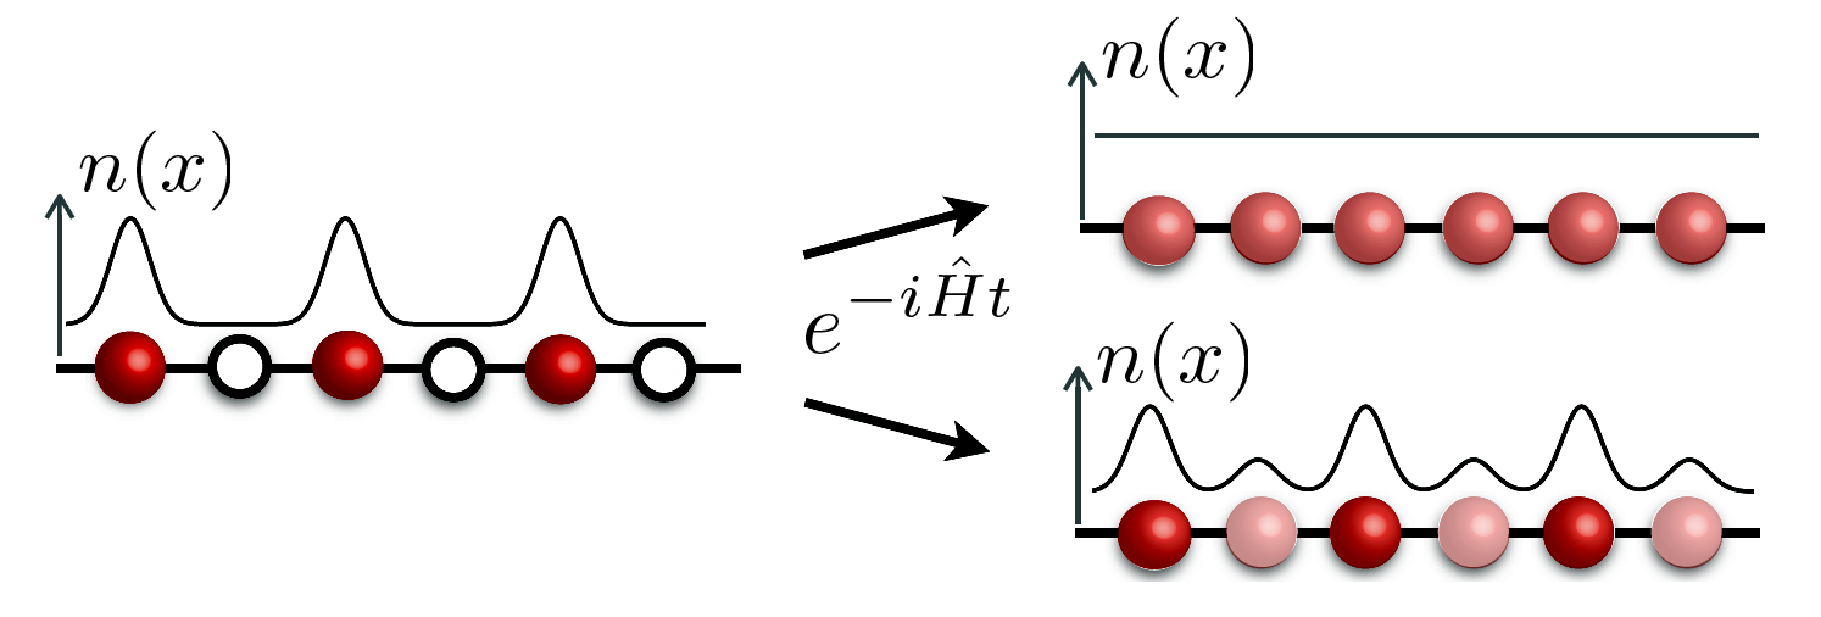
\includegraphics[width=0.95\textwidth]{abanin_thermalization_scheme.pdf}}
\caption{
Shematski prikaz razlike med unitarnim časovnim razvojem netipične začetne konfiguracije interagirajočih delcev v ergodičnem in MBL režimu, kjer je netipičnost dosežena z alternirajočo zasedenostjo mest na kristalni verigi.
 V prvem primeru sistem sčasoma relaksira proti ravnovesni enakomerni porazdelitvi delcev, medtem ko se tovrstna relaksacija v MBL fazi ne zgodi - tudi po dolgem času sistem ohrani spomin na netipičnost začetnega stanja. Slika je bila vzeta iz Ref.~\cite{abanin2018ergodicity}. 
}
\label{fig:abanin_thermalization}
\end{figure}
\end{minipage}
ETH lastna stanja niso termalna. Informacija o prekrivanju začetnega stanja z lastnimi funkcijami hamiltonke se v diagonalnih matričnih elementih ohrani tudi po dolgem
  času. Pravimo, da MBL sistemi ohranjajo `spomin' na začetno konfiguracijo. Hkrati iz odsotnosti termalizacije sledita tudi ničelna prevodnost in ničelni transport v MBL sistemih. Za uspešen potek termalizacije sta namreč potrebna transport delcev in energije med različnimi deli sistema. \\\\
Zgoraj opisana odsotnost termalizacije v MBL sistemih vpliva tudi na spektralne lastnosti njihovih modelskih hamiltonk, ki se bistveno razlikujejo od lastnosti ergodičnih sistemov. Med prvimi sta nastop MBL skozi prizmo spektralnih statistik preučevala Oganesyan in Huse~\cite{PhysRevB.75.155111}, podoben pristop pa pri presoji ergodičnosti oziroma lokaliziranosti konkretnih modelskih sistemov v poglavju~\ref{statisticne_lastnosti} uporabljamo tudi mi. Poglavitne koncepte zato podrobneje uvedemo kasneje, tu pa le na kratko povzamemo bistvo - namreč, da so lastnosti energijskih spektrov ergodičnih in MBL sistemov univerzalne in kvalitativno različne~\cite{mehta2004random}~\cite{Atas_Distribution_PhysRevLett.110.084101}~\cite{d2016quantum}. Vrednosti različnih spektralnih opazljivk, v nalogi denimo preučujemo porazdelitev \emph{razmikov} med sosednjimi energijskimi nivoji in statistiko \emph{razmerij razmikov} med sosednjimi energijskimi nivoji~\cite{PhysRevB.75.155111}, se zato v obeh režimih razlikujejo in omogočajo presojo ergodičnosti oziroma lokaliziranosti sistema. Primer tovrstne presoje na podlagi statistike razmikov sosednjih energijskih nivojev prikazuje Slika~\ref{fig:unfolding_demo}.
\begin{figure}[H]
\centering{
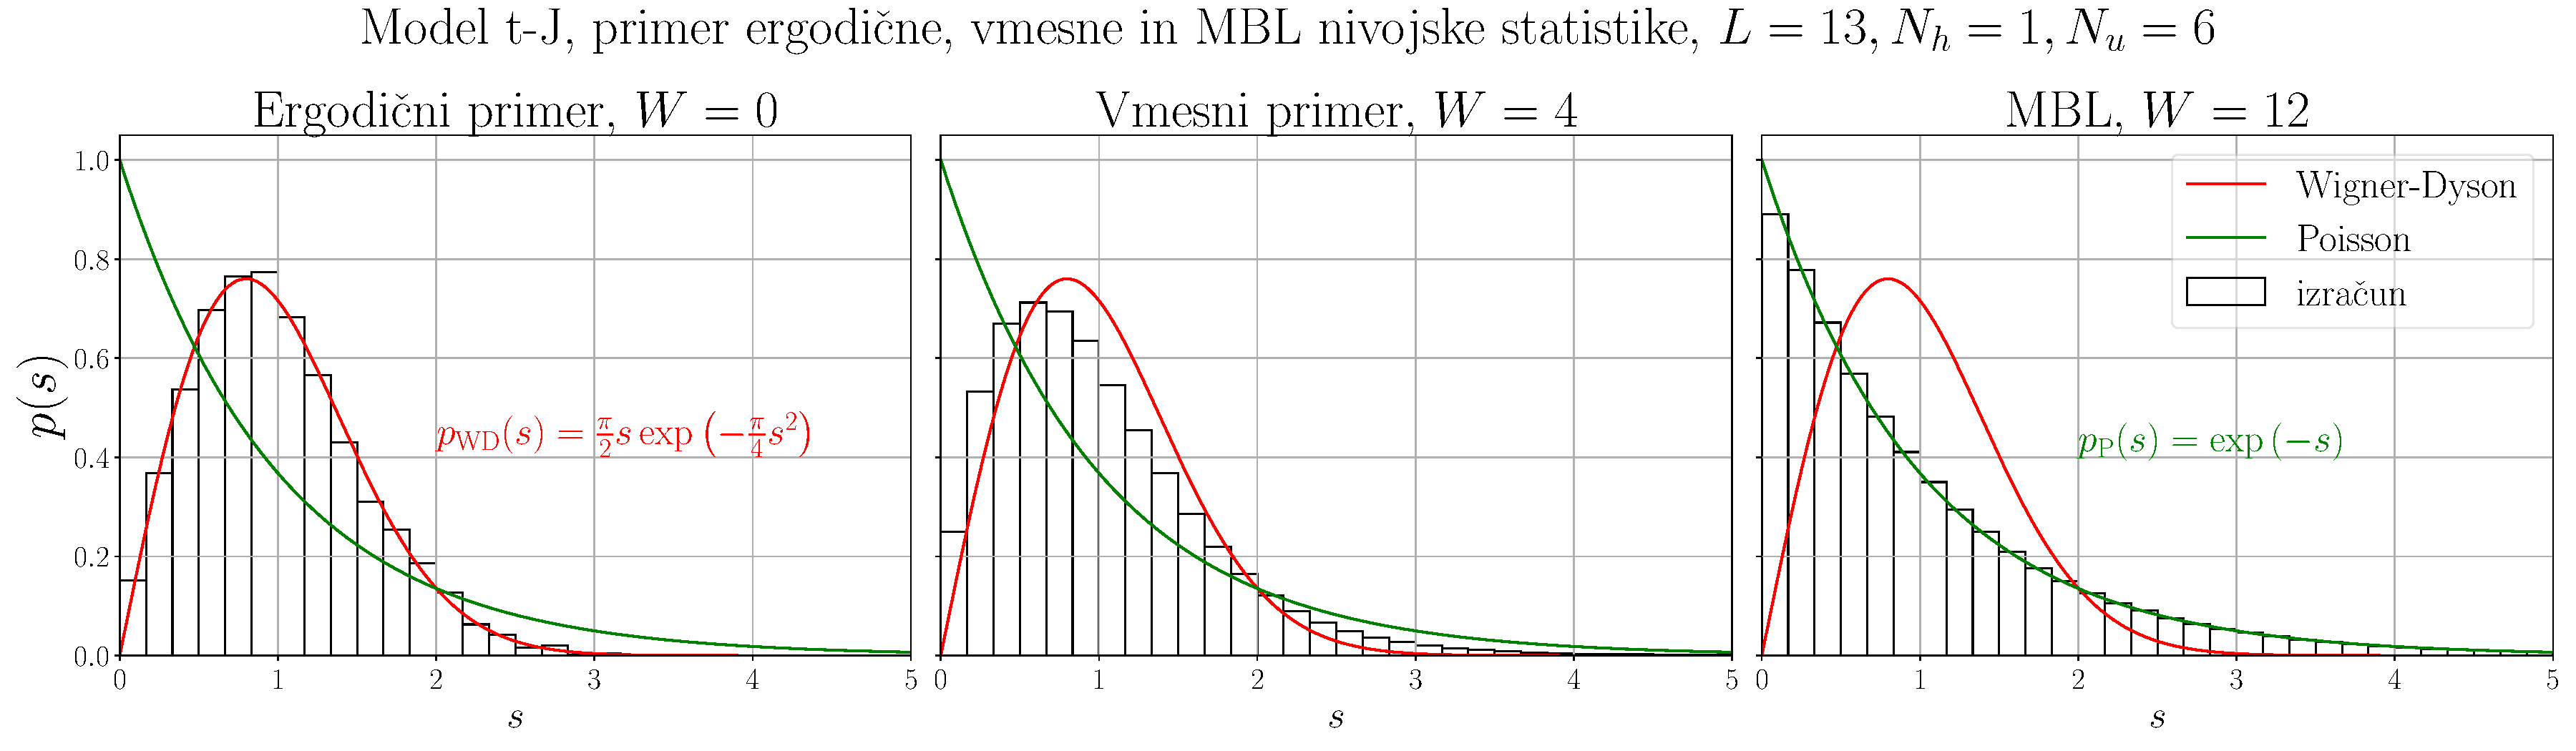
\includegraphics[trim=0 0 0 50,clip,width=1\textwidth]{unfolding_demo_three_slo.pdf}}
\caption{Ilustrativen primer uporabe spektralne statistike za presojo ergodičnosti oziroma lokaliziranosti sistema. Prikazana je porazdelitev statistike sosednjih energijskih nivojev za model $t$-$J$ z naključnim potencialnim neredom, v katerem pride do prehoda med ergodično in MBL fazo. Formalno je model vpeljan v poglavju~\ref{spinfull}. V ergodičnem primeru se mora statistika ujemati z rdečo Wigner-Dysonovo krivuljo, v MBL primeru pa z zeleno Poissonovo krivuljo. Razlogi so razloženi v poglavju~\ref{statisticne_lastnosti}.
}
\label{fig:unfolding_demo}
\end{figure}
\noindent
\begin{minipage}[t]{0.65\textwidth}
\noindent \\
Pomemben kriterij za razločanje med ergodičnimi in MBL sistemi je tudi skaliranje prepletenostne entropije lastnih stanj sistema. Prepletenostna entropija podsistema A je definirana kot von Neumannova entropija reducirane gostotne matrike $\hat{\rho}_\mathrm{A}$ podsistema A: 
\begin{equation}\label{eq:entanglement}
S_\mathrm{ent}\left(A\right)=-\mathrm{Tr}\left\{ \hat{\rho}_\mathrm{A}\log \hat{\rho}_\mathrm{A}\right\}.
\end{equation}
Pri tem smo privzeli, da je celoten sistem razdeljen na dva podsistema, denimo A in B, kot prikazuje Slika~\ref{fig:nandkishore_huse_subsystems}. Reducirano gostotno matriko $\hat{\rho}_\mathrm{A}$ dobimo z delno sledjo  po prostostnih stopnjah podsistema B nad gostotno matriko $\hat{\rho}$:
\begin{equation}
\hat{\rho}_\mathrm{A}=\mathrm{Tr}_\mathrm{B}\	 \hat{\rho}.
\end{equation}\\
\end{minipage}\hfill
\begin{minipage}[t]{0.32\textwidth}
\begin{figure}[H]
\centering{
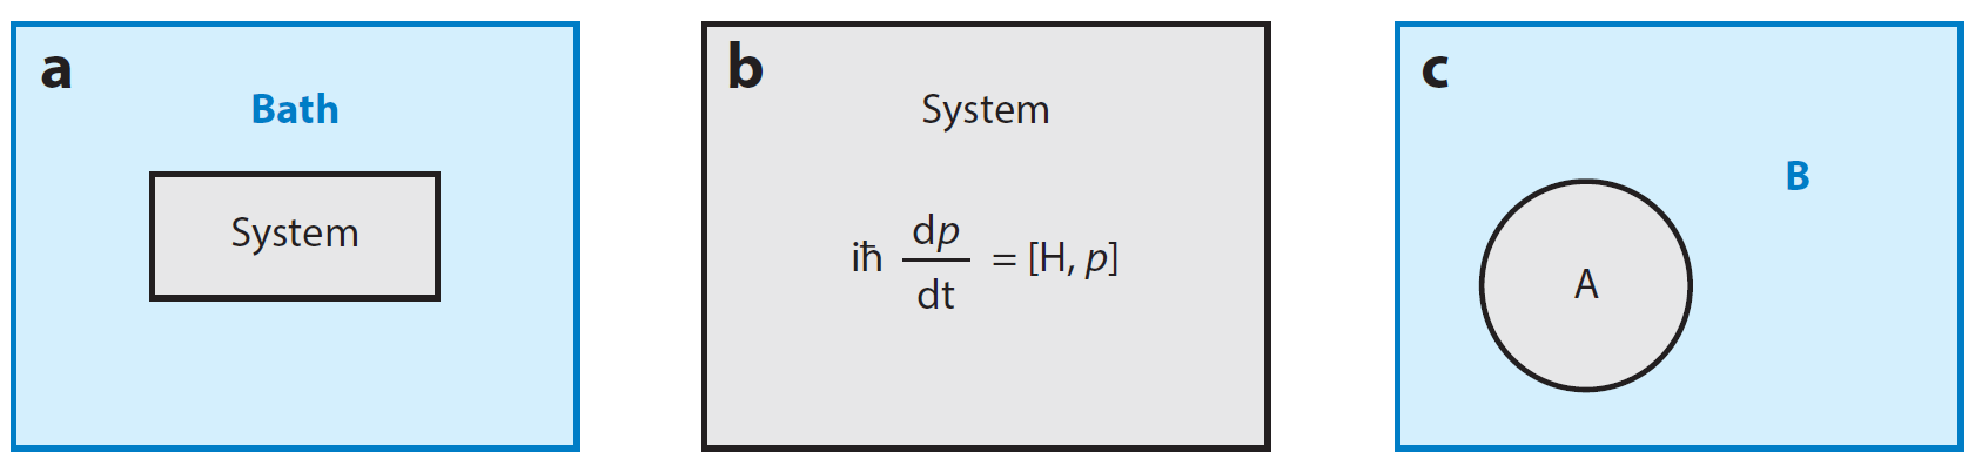
\includegraphics[trim=660 0 0 0,clip, width=0.87\textwidth]{nandkishore_huse_reservoir.pdf}}
\caption{
Shema v pomoč k vpeljavi pojma prepletenostne entropije. Izoliran kvantni sistem razdelimo na podsistema A in B.
Slika je bila povzeta po Ref.~\cite{nandkishore2015many}. 
}
\label{fig:nandkishore_huse_subsystems}
\end{figure}
\end{minipage}
Za lastna stanja $\ket{\alpha}$ mora biti reducirana gostotna matrika $\hat{\rho}_\mathrm{A}^\alpha=\mathrm{Tr}_\mathrm{B}\ \ket{\alpha}\bra{\alpha}$ ob predpostavki veljavnosti ETH podobna termalni gostotni matriki podsistema A, saj se pričakovane vrednosti opazljivk
  sistema 
ujemajo s tistimi v termalnem stanju.
To pomeni, da je za lastna stanja v ergodičnih sistemih $S_\mathrm{ent}(\mathrm{A})$ enaka termodinamski entropiji podsistema A in je zato ekstenzivna - skalira z velikostjo
podsistema A, $S_\mathrm{ent}(A)\propto \mathrm{vol}(A).$ Temu pravimo \emph{volumsko skaliranje} prepletenostne entropije (ang.~\emph{volume-law scaling}). \\\\Obnašanje v 
MBL sistemih je drugačno, saj so njihova lastna stanja v \emph{celotnem spektru} šibko prepletena. Numerične študije~\cite{serbyn2013local}~\cite{bauer2013area} nakazujejo, da je skaliranje prepletenostne entropije \emph{površinsko} (ang.~\emph{area-law scaling}) oziroma sorazmerno površini roba podsistema A, $S_\mathrm{ent}(A)\propto \mathrm{vol}(\partial A)$. Z numerično analizo prepletenostne entropije v konkretnih modelskih sistemih se ukvarjamo v poglavju~\ref{prepletenostna_numericno}.

% Kot smo opisali v predhodnem poglavju, so v ergodičnih sistemih večdelčna lastna stanja termalna, kar v izoliranem sistemu dovoljuje relaksacijo poljubnega začetnega stanja proti ravnovesni vrednosti - sistem lahko \emph{sam sebi služi kot toplotna kopel}. V MBL sistemih je drugače, saj zanje ETH ne velja in lastna stanja niso termalna. Tudi po dolgem času so pričakovane vrednosti lokalnih opazljivk namesto s termalnimi vrednostmi določene s podrobnostmi lokalnih konfiguracij začetnih stanj. Začetna stanja se z gostotno matriko v bazi lastnih stanj zapišejo kot $\hat{\rho}=\sum\limits_{\alpha,\beta}\rho_{\alpha\beta}\ket{\alpha}\bra{\beta}.$ V ergodičnem primeru se vsa informacija o prekrivanju začetnega stanja z lastnimi funkcijami sistema po dolgočasovnem razvoju porazgubi, oziroma točneje rečeno, preplete s preostalimi lokalnimi prostostnimi stopnjami. Izvendiagonalni matrični elementi se zaradi dekoherence namreč kot v En.~\eqref{eq:ergodicnost_kvantno} po dolgem času izpovprečijo, diagonalni elementi pa ostanejo nespremenjeni. Ker so lastna stanja v ergodičnem primeru termalna, vodi unitarna hamiltonska dinamika do termalnega ravnovesja. V MBL primeru dekoherenca izvendiagonalnih matričnih elementov sicer tudi zabriše informacijo o naravi začetnega stanja, 
% vendar se slednja ohrani v diagonalnih elementih gostotne matrike. Ker v MBL primeru lastna stanja niso termalna, so diagonalni matrični elementi določeni z lokalnimi značilnostmi lastnih stanj.  
%TO DO: 
%KAJ NAJ BO V UVODU: -> GIBALNE ENAČBE ZA VEČDELČNE SISTEME (VON NEUMANN) CHECK
%RAZLAGA IZOLACIJE IN KAJ JE SPLOH ERGODIČNOST V KVANTNEM SISTEMU (GLEJ D ALLESSIO) CHECK
%INTERAKCIJE -> POMEN: KONČNA GOSTOTA ENERGIJE, KAKO JE TO DRUGAČE OD ANDERSONA -> daj to najprej po uvodnem odstavku, VIRI: Basko, Oganesyan, Huse, CHECK

%NAJPREJ ZA UVOD: ETH, INTEGRABILNI, MBL -> 4 lastnosti: STATISTIKA, NEERGODIČNOST V ČASU , TRANSPORT 0, ENTENGLEMENT ŠE TREBA
%ENAČBE ZA ZAPRTE KVANTNE SISTEME -> ČASOVNI RAZVOJ:  CHECK
%Nandkishore, Huse: kje se to lahko študira: sistemi z mobilnimi delci, glej poglavje 4.2

\chapter{Modeli in metode}\label{modelimetode}
Do sedaj smo se pri obravnavi pojavov MBL omejili na opis lastnosti netermalizirajočih sistemov, zdaj pa nas zanimajo konkretni modeli, v katerih je termalizacija ob prisotnosti interakcij onemogočena. Ker odsotnost transporta preprečuje termalizacijo, je Andersonov izolator, obravnavan v poglavju~\ref{anderson}, primerno izhodišče za konstrukcijo modelov MBL. Obravnava fermionskih modelov brez spinskih prostostnih stopenj (ang.~\emph{spinless fermions} v nadaljevanju \emph{brezspinski} fermioni) v poglavju~\ref{Heis_spinless} služi predvsem kot splošen pregled področja in nekaterih ključnih rezultatov. Predstavljena sta enodimenzionalni model $t$-$V$ z dodatkom nereda in enodimenzionalni Heisenbergov model XXZ z naključnim magnetnim poljem. Zaradi obstoja Jordan-Wignerjeve transformacije, ki jo vpeljemo v En.~\eqref{eq:Jordan-Wigner}, sta energijska spektra obeh modelov identična. 
Izmed fermionskih modelov s spinskimi prostostnimi stopnjami (ang.~\emph{spinful fermions}, v nadaljevanju \emph{spinski} fermioni) sta v poglavju~\ref{spinfull} podrobjene predstavljena Hubbardov model in model $t$-$J$ z dodanim neredom. 
% Poleg predstavitve modela je podana tudi izpeljava preslikave med Hubbardovim modelom in modelom $t$-$J$. 
V poglavju~\ref{diagonalizacija_metoda} je opisana točna diagonalizacija modelskih hamiltonk, na kateri temelji presoja ergodičnosti oziroma lokaliziranosti v poglavjih~\ref{statisticne_lastnosti} in~\ref{prepletenostna_numericno}.
\section{Fermionski modeli brez spinskih prostostnih stopenj}
\label{Heis_spinless}
Eden izmed prvih in do danes najpogosteje uporabljanih modelov fizike sistemov MBL je enodimenzionalni model $t$-$V$ z dodanim neredom. Gre za enodimenzionalno verigo brezspinskih fermionov z interakcijami med najbližjimi sosedi in lokalnim neredom Andersonovega tipa. Pri nadaljnji razpravi bomo zavoljo jedrnatosti s poimenovanjem $t$-$V$ v mislih vselej privzeli tudi prisotnost nereda. \\\\Model dobimo, če v hamiltonko Andersonovega modela, podano z En.~\eqref{eq:Anderson_ham}, vključimo medsosedske interakcije, katerih velikost določa parameter $V$:
\begin{equation}\label{eq:tV}
H=-t\sum\limits_i\left(c^\dagger_i c_{i+1} + \mathrm{h.c.}\right) + V\sum\limits_i n_in_{i+1} + \sum\limits_i u_in_i.
\end{equation} 
Tako kot v Andersonovem modelu so vrednosti naključnih potencialov $u_i$ porazdeljene enakomerno na intervalu $[-W,W]$ v skladu z En.~\eqref{eq:and_prob}, v kateri je $W$ parameter velikosti nereda. V tem primeru sta pri ničelni temperaturi in polovični zasedenosti pasu možna  dva režima, ki ju ločimo glede na velikost \emph{parametra anizotropije } $\Delta=V/(2t)$.  Za šibko oziroma zmerno interakcijo v primeru $\Delta<1$ je sistem prevodnik, v režimu močne interakcije pri $\Delta\geq 1$ pa izolator~\cite{prelovvsek2017density}. \\\\
Leta 2007 sta s točno diagonalizacijo končnih sistemov Oganesyan in Huse~\cite{PhysRevB.75.155111} v modelu $t$-$V$  nakazala možnost obstoja MBL faze tudi pri neskončnih temperaturah. \\\\
Model $t$-$V$ lahko z uporabo Jordan-Wignerjeve transformacije preslikamo na model anizotropne Heisenbergove spinske verige spinov $S=1/2$  z naključnimi lokalnimi vrednostmi magnetnega polja $h_i$ vzdolž smeri $z$. Hamiltonka modela, ki ga sicer imenujemo tudi model XXZ z naključnim magnetnim poljem, je podana z 
\begin{equation}\label{eq:XXZ}
H=J\sum\limits_i\left[\frac{1}{2}\left(S_{i+1}^+S_i^- + S_i^+S_{i+1}^-\right) + \Delta S_{i+1}^zS_i^z\right] + \sum\limits_i h_i S_i^z.
\end{equation}
Tu so $S_i^+, S_i^-$ in $S_i^z$ standardni operatorji za spin $S=1/2$ na $i$-tem mestu v enodimenzionalni spinski verigi. Izmenjalna konstanta se z modelskimi parametri modela $t$-$V$ izrazi kot $J=2t$~\cite{prelovvsek2017density}, parameter anizotropije $\Delta$ pa smo definirali že zgoraj. Fermionski skakalni člen v modelu XXZ ustreza izmenjalnemu členu, medtem ko medsosedska fermionska interakcija ustreza členu s parametrom $\Delta$. V odsotnosti naključnega člena je model rešljiv z uporabo Bethejevega nastavka~\cite{karabach1997introduction}. Naključne vrednosti magnetnega polja so porazdeljene enakomerno na intervalu $[-2W,2W]$.  Jordan-Wignerjevo transformacijo v eni dimenziji podajajo zveze
\begin{equation}\label{eq:Jordan-Wigner}
S_i^+=c^\dagger_i\prod_{j<i}\mathrm{e}^{\iu\pi n_j}, \hspace{5mm} S_i^-=\left(\prod_{j<i}\mathrm{e}^{-\iu\pi n_j}\right)c_i,\hspace{5mm} S^z_i= n_i - \frac{1}{2}.
\end{equation}  
Limita $\Delta\to0$ ustreza neinteragirajočemu primeru, ko lahko spinski model preslikamo na model prostih fermionov v naključnem potencialu, torej na Andersonov model, ki smo ga obravnavali v poglavju~\ref{anderson}. Kot smo tedaj pokazali, so v eni dimenziji vsa lastna stanja sistema lokalizirana za vsakršno končno vrednost parametra nereda $W$. \\\\
Interakcijo modeliramo s končnimi vrednostmi $\Delta$. Vpliv prepleta interakcij in nereda na nastop MBL faze je shematsko prikazan na Sliki~\ref{fig:XXZ_t_V}. Pri neki fiksni vrednosti parametra $W$ so vsa lastna stanja sistema lokalizirana, če je velikost interaktivne sklopitve $J_z=J\Delta$ manjša od neke kritične in od nereda odvisne vrednosti $J_z^*(W).$ Če nered ni prevelik, ima $J_z^*$ končno vrednost in tedaj nadkritične vrednosti $J_z$ omogočajo termalizacijo. Podobno pri fiksni vrednosti $J_z$ obstaja kritična vrednost parametra nereda $W^*$, nad katero so vsa stanja sistema lokalizirana. Medtem ko so stanja na robovih pasu lokalizirana tudi pri podkritičnih vrednostih nereda $W<W^*$, nakazujejo numerične študije~\cite{luitz2015many} na obstoj delokaliziranih stanj v sredini pasu. V nasprotju z Andersonovim modelom torej ob prisotnosti interakcij \emph{večdelčni} rob mobilnosti obstaja že v eni dimenziji.  
\begin{figure}[H]
\floatbox[{\capbeside\thisfloatsetup{capbesideposition={left,center},capbesidewidth=7cm}}]{figure}[\FBwidth]
{\caption{\textbf{a)} in \textbf{b)} Shematski prikaz modela XXZ oziroma modela $t$-$V$ v eni dimenziji in ekvivalence med njima. Rumene puščice označujejo interakcijo. \textbf{c)} Prehod med MBL in ergodično fazo pri fiksnem $W$ v odvisnosti od $J_z$. Točka $J_z=0$ ustreza Andersonovemu izolatorju. \textbf{d)} Prehod med ergodično in MBL fazo kot funkcija parametra nereda $W$. Lokalizacija nastopi nad kritično vrednostjo $W^*$. Slika je bila vzeta iz Ref.~\cite{abanin2018ergodicity}. }\label{fig:XXZ_t_V}}
{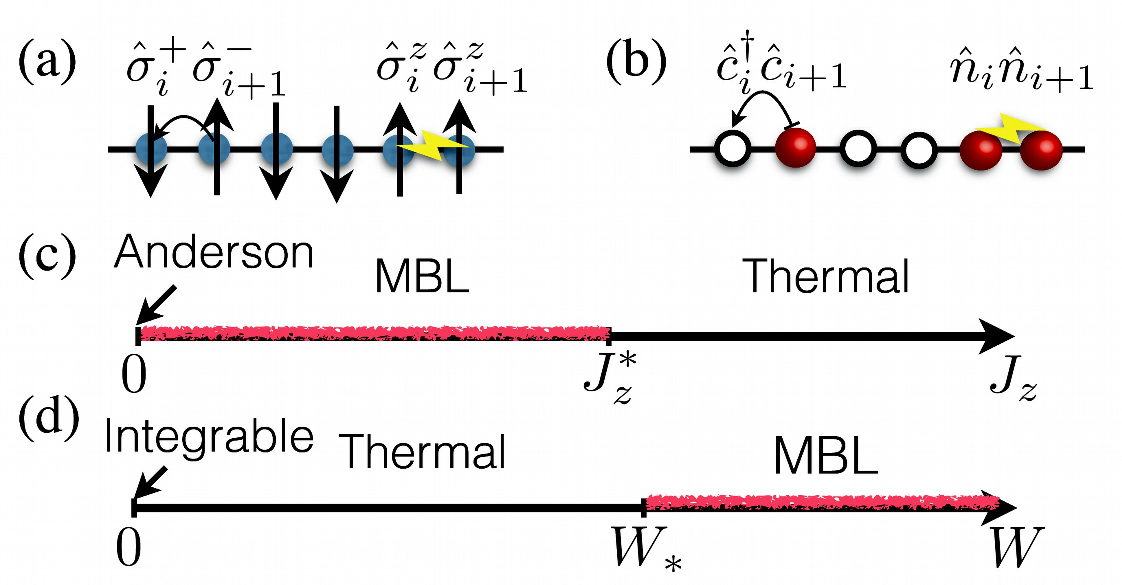
\includegraphics[width=0.5\textwidth]{scheme_XXZ_t_V.pdf}}
\end{figure} 
\noindent
V izotropnem primeru za $\Delta=1$ in $J=1$ znaša numerično izračunana kritična vrednost parametra nereda $W^*\approx 3.5.$ Pri tej vrednosti nastopi prehod med ergodično in lokalizirano fazo~\cite{pal2010many}. Model XXZ je bil podrobno preučevan tudi v enem izmed prelomnih del s področja~\cite{vznidarivc2008many}, v katerem je bila pokazana logaritemska rast prepletenostne entropije v odvisnosti od časa za začetno produktno (neprepleteno) stanje dveh podsistemov na spinski verigi. To nakazuje na kvalitativno razliko med Andersonovimi izolatorji in MBL sistemi, saj v prvih prepletenostna entropija lahko narašča za kratke čase, po dolgem času pa doseže konstantno vrednost.  

% Pri fiksnih vendar ne prevelikih vrednostih parametra $W$ so vsa lastna stanja sistema lokalizirana, če je sklopitev vzdolž osi $z$ šibkejša od neke kritične vrednosti, $\abs{J_z}<J_z^*(W)$, kjer je $J_z=J\Delta$. Podobno je pri fiksni
\section{Fermionski modeli s spinskimi prostostnimi stopnjami}
\label{spinfull}
V tem poglavju v obravnavo fermionskih sistemov vključimo tudi spinske prostostne stopnje in podrobneje predstavimo model $t$-$J$, ki ga numerično preučujemo v poglavjih~\ref{statisticne_lastnosti} in~\ref{prepletenostna_numericno}. Gre za model, ki v limiti močne meddelčne interakcije ustreza fiziki nizkoenergijskih stanj Hubbardovega modela. Zavoljo formalne vpeljave pojmov je najprej na kratko predstavljen Hubbardov model, medtem ko se modelu $t$-$J$ posvetimo podrobneje, saj ga v nadaljnjih poglavjih preučujemo tudi numerično. V Dodatku~\ref{tj_hubb_preslikava} je podana izpeljava preslikave med modeloma, in sicer tako v primeru urejenega sistema kot v prisotnosti različnih tipov nereda.  Posebej nas zanimata \emph{potencialni} in \emph{spinski} nered, torej nereda, ki se sklapljata z nosilci naboja oziroma spini. V tem vrstnem redu smo oba tipa nereda že srečali v En.~\eqref{eq:tV} in~\eqref{eq:XXZ}.\\\\
\subsection{Hubbardov model}
Kot izhodišče za obravnavo modela $t$-$J$ najprej formalno uvedemo Hubbardov model, iz katerega prvega izpeljemo. Za splošen tip nereda je hamiltonka Hubbardovega modela podana z 
\begin{equation}\label{eq:hubbard_main_text}
H=H_t + H_U+ H_\mathrm{dis}=-t\sum\limits_{\langle ij \rangle, \sigma}\left(c^\dagger_{i,\sigma} c_{j\sigma} + c^\dagger_{j\sigma}c_{i\sigma}\right) + U\sum_i n_{i\uparrow}n_{i\downarrow} +  \sum\limits_{i,\sigma} h_{i,\sigma} n_{i, \sigma}. 
\end{equation}
Pri tem  $\langle ij \rangle$ označuje vsoto po najbližjih sosedih, $\sigma$ pa vsoto po projekcijah spina $S=1/2$ na os $z$. Fermionski kreacijski in anihilacijski operatorji $c^\dagger_{i,\sigma}, c_{i,\sigma}$ ustvarijo oziroma uničijo delec z dano projekcijo spina $\sigma$ na $i$-tem mestu v kristalni rešetki.  V Hubbardovi hamiltonki tako kot vselej do sedaj skakalni člen $H_t$ opisuje skakanje elektronov med sosednjimi mesti v kristalni rešetki, kjer je $t$ verjetnost za tovrstno tuneliranje. Interakcijski člen $H_U$ modelira coulombski odboj med elektroni in ob dvojni zasedenosti mesta povzroči energijski prirastek $U.$ V členu $H_\mathrm{dis},$ ki modelira prispevek nereda v sistemu, so  $h_{i,\sigma}$ v skladu z neko verjetnostno porazdelitvijo izžrebane naključne vrednosti, pri čemer sta porazdelitvi za posamezni projekciji spina v splošnem lahko različni. \\\\
Pri zapisu Hubbardove hamiltonke smo upoštevali t.i.~\emph{bazo zasedenosti posameznih mest} (ang.~\emph{site-occupational basis}), kjer so na $i$-tem mestu v kristalni rešetki možna štiri stanja, in sicer 
\begin{equation}\label{eq:hubstates}
\ket{\psi_{i_0}}=\ket{0}_i, \hspace{5mm} \ket{\psi_{i_1}}=\ket{\uparrow}_i,\hspace{5mm} \ket{\psi_{i_{2}}}=\ket{\downarrow}_i, \hspace{5mm} \ket{\psi_{i_{3}}}=\ket{\uparrow\downarrow}_i
\end{equation}
V prvem stanju na $i$-tem mestu ni elektrona oziroma se tam nahaja vrzel, naslednji dve stanji pa ustrezata prisotnosti elektrona s spinom $1/2$ in eno izmed dveh možnih projekcih spina na os $z$. Zadnje stanje pomeni zasedenost mesta z dvema elektronoma z nasprotnim spinom. \\\\
Za številsko gostoto delcev in skupno projekcijo spina na os $z$ na $i$-tem mestu  veljata zvezi
\begin{equation}\label{eq:hubb_zveze}
n_i=n_{i,\uparrow}+n_{i,\downarrow},\hspace{5mm} S_i^z=\frac{1}{2}\left(n_{i,\uparrow} - n_{i,\downarrow}\right).
\end{equation}
Če želimo v En.~\eqref{eq:hubbard_main_text} modelirati prispevek nereda, ki se sklaplja le z nosilci naboja, ne pa tudi njihovimi spinskimi prostostnimi stopnjami, potem za porazdelitev $h_{i,\sigma}$ predpišemo $h_{i, \uparrow}=h_{i,\downarrow}.$ Tak tip nereda smo srečali denimo v En.~\eqref{eq:tV}. Nered, ki se sklaplja s spinskimi prostostnimi stopnjami in je odvisen od projekcije spina na os $z$, pa dobimo prek predpisa $h_{i,\uparrow}=-h_{i,\downarrow}.$ Ta tip nereda poznamo iz En.~\eqref{eq:XXZ}.
\subsection{Model $t$-$J$}
V magistrski nalogi z numeričnimi metodami preučujemo model $t$-$J$~\cite{spalek2007tj} s periodičnimi robnimi pogoji na enodimenzionalni verigi. V limiti močnega coulombskega odboja $U$ model opisuje fiziko nizkoenergijskih stanj Hubbardovega modela. Ker je za velike $U$ dvojna zasedenost mest energijsko neugodna, je v modelu $t$-$J$ prepovedana in so za razliko od En.~\eqref{eq:hubstates} na vsakem mestu možna le tri stanja: 
\begin{equation}\label{eq:tjstates}
\ket{\psi_{i_0}}=\ket{0}_i, \hspace{5mm} \ket{\psi_{i_1}}=\ket{\uparrow}_i,\hspace{5mm} \ket{\psi_{i_{-1}}}=\ket{\downarrow}_i.
\end{equation}
Sledeč izpeljavi, navedeni v Dodatku~\ref{tj_hubb_preslikava}, dobimo za model $t$-$J$ v prisotnosti nereda hamiltonko
\begin{equation}\label{eq:tJ_ham}
\begin{split}
H&=-t\sum\limits_{i, \sigma} \left(\tilde{c}_{i,\sigma}^\dagger\tilde{c}_{i+1,\sigma} + c.c. \right) + J\sum\limits_i \left(\vec{S}_i\cdot \vec{S}_{i+1} - \frac{n_i n_{i+1}}{4}\right) + \sum\limits_i h_iS_i^z + \sum\limits_{i,\sigma} u_i n_{i,\sigma}=  \\
&=
H_t + H_J + H_h + H_u.
\end{split}
\end{equation}
Pri tem so $\tilde{c}_{i,\sigma}^\dagger$ in  $\tilde{c}_{i,\sigma}$ \emph{projicirani} fermionski kreacijski in anihilacijski operatorji, ki jih vpeljemo v skladu s predpisom 
\begin{equation}
\tilde{c}_{i,\sigma}^\dagger=c_{i,\sigma}^\dagger(1-n_{i,-\sigma}) \hspace{5mm}\tilde{c}_{i,\sigma}=(1-n_{i,-\sigma})c_{i,\sigma}.
\end{equation}
Tako definirani kreacijski operatorji lahko na $i$-tem mestu v kristalni verigi ustvarijo delec z dano $z$-projekcijo spina $\sigma$ samo v primeru, ko se na mestu predhodno še ne nahaja delec z nasprotno projekcijo spina na os $z$. Na ta način upoštevamo prepoved dvojne fermionske zasedenosti mest. Ob upoštevanju omenjene prepovedi je vloga člena $H_t$ sicer enaka kot v Hubbardovem modelu. \\\\ 
Meddelčno interakcijo v hamiltonki modelira Heisenbergov izmenjalni člen $H_J$, pri čemer za spinske operatorje za spin $S=1/2$ velja $\vec{S}_i\cdot \vec{S}_{j}=\frac{1}{2}\left(S_i^+S_j^- + S_i^-S_j^+\right) + S_i^zS_j^z$. Pri numeričnih simulacijah za izmenjalno interakcijo $J$ vselej privzamemo izotropijo. V Dodatku~\ref{tj_hubb_preslikava} pokažemo, da se $J$ z modelskimi parametri Hubbardovega modela izraža kot $J=\frac{4t^2}{U}.$ 
Delovanje členov $H_t$ in $H_J$ je shematsko prikazano in razloženo na Sliki \ref{fig:tJ_scheme}. \\\\
S členom $H_h$ v hamiltonki modeliramo prispevek naključnega magnetnega polja v smeri osi $z$, ki se zeemansko sklaplja s 
spinskimi prostostnimi stopnjami, pri čemer je $h_i$ velikost naključno izžrebanega magnetnega polja na $i$-tem mestu v kristalni rešetki. Podobno člen $H_u$ modelira potencialni nered, ki se sklaplja z vrzelmi v kristalni rešetki, $u_i$ pa je naključno izžrebana vrednost energije vrzeli, ki se nahaja na $i$-tem mestu v kristalni rešetki. Vrednosti $w_i$ in $h_i$ tipično izžrebamo v skladu s škatlasto verjetnostno porazdelitvijo, kot prikazuje Slika \ref{fig:prob_dist}, na kateri sta $W$ in $H$	 parametra 
nereda, s katerima določamo velikost spinskega in vrzelnega potencialnega nereda. Prehod med ergodično in MBL fazo
v modelu zasledujemo kot funkcijo velikosti obeh omenjenih parametrov.\\\\
V besedilu velikost sistema označuje $L$, $N_h$ število vrzeli, $N_u$ pa število spinov $1/2$ s projekcijo spina navzgor. Pri analizi se vselej osredotočimo na podprostor hamiltonke, podane z En. \eqref{eq:tJ_ham}, s fiksnim številom vrzeli in ničelno skupno projekcijo spina na os $z$, $S^z=0$. Stanja s skupno projekcijo spina nič so v hamiltonki najštevilčnejša, zato gre za statistično najbolj zastopan sektor. Vse funkcije z dobro določenim spinom imajo namreč tudi projekcijo v podprostoru s $S^z=0$. Število stanj v podprostoru s fiksnim številom vrzeli in ničelnim spinom določimo s pomočjo kombinatorike - najprej prešteje{}mo število razporeditev $N_h$ vrzeli na $L$ mest v verigi, kar nato pomnožimo še s številom razporeditev $N_u$ spinov na preostalih $L-N_h$ mest. Število stanj torej podaja zveza
\begin{equation}\label{eq:nstat}
N_\mathrm{stat}=\binom{L}{N_h}\binom{L-N_h}{N_u}.
\end{equation}
Odvisnost števila stanj od velikosti sistema in števila vrzeli je za primer $S^z=0$ prikazana na Sliki~\ref{fig:tJ_num_states}.
\newpage
\begin{figure}[H]
\floatbox[{\capbeside\thisfloatsetup{capbesideposition={left,center},capbesidewidth=5cm}}]{figure}[\FBwidth]
{\caption{Shematski prikaz modela $t$-$J$ na verigi z $L=7$ mesti, $N_h=2$ vrzelma in $N_u=2$ navzgor obrnjenima spinoma in odprtimi robnimi pogoji.	 $J$ označuje velikost izmenjalne interakcije med spini sosednjih elektronov, ki obrne par nasprotno obrnjenih spinov (ang.~\emph{spin-flips}). Verjetnost za tuneliranje elektrona na prazno mesto označuje $t$. }\label{fig:tJ_scheme}}
{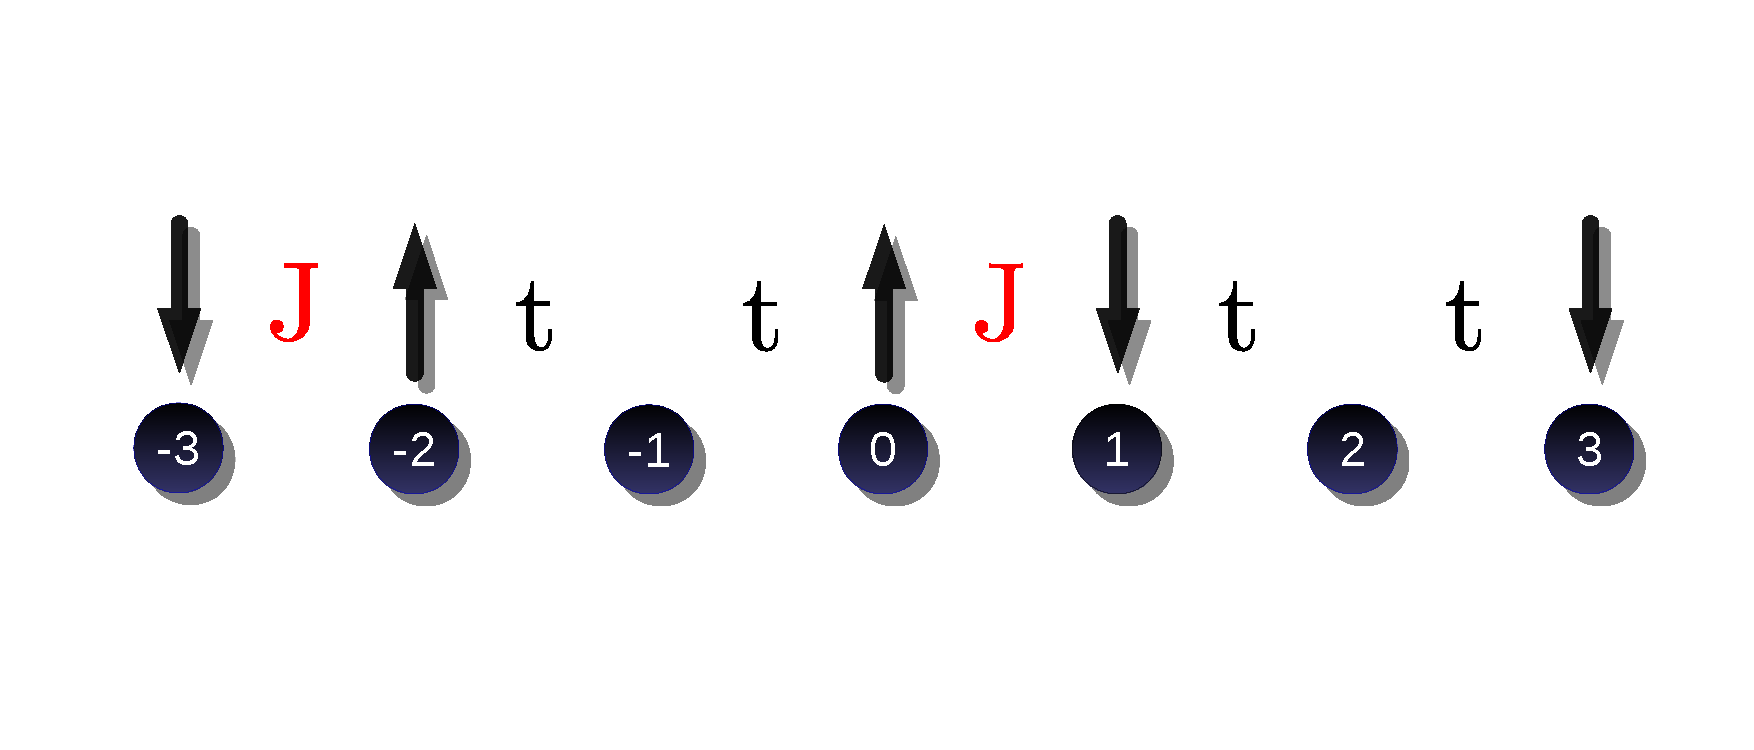
\includegraphics[width=0.62\textwidth]{tJ_scheme.pdf}}
\end{figure}
\begin{figure}[H]
\floatbox[{\capbeside\thisfloatsetup{capbesideposition={left,center},capbesidewidth=5cm}}]{figure}[\FBwidth]
{\caption{Naključne vrednosti magnetnega polja $w_i$ in potenciala $h_i$ tipično izžrebam v skladu s škatlasto verjetnostjo porazdelitvijo, kjer sta $W$ in $H$ parametra nereda. }\label{fig:prob_dist}}
{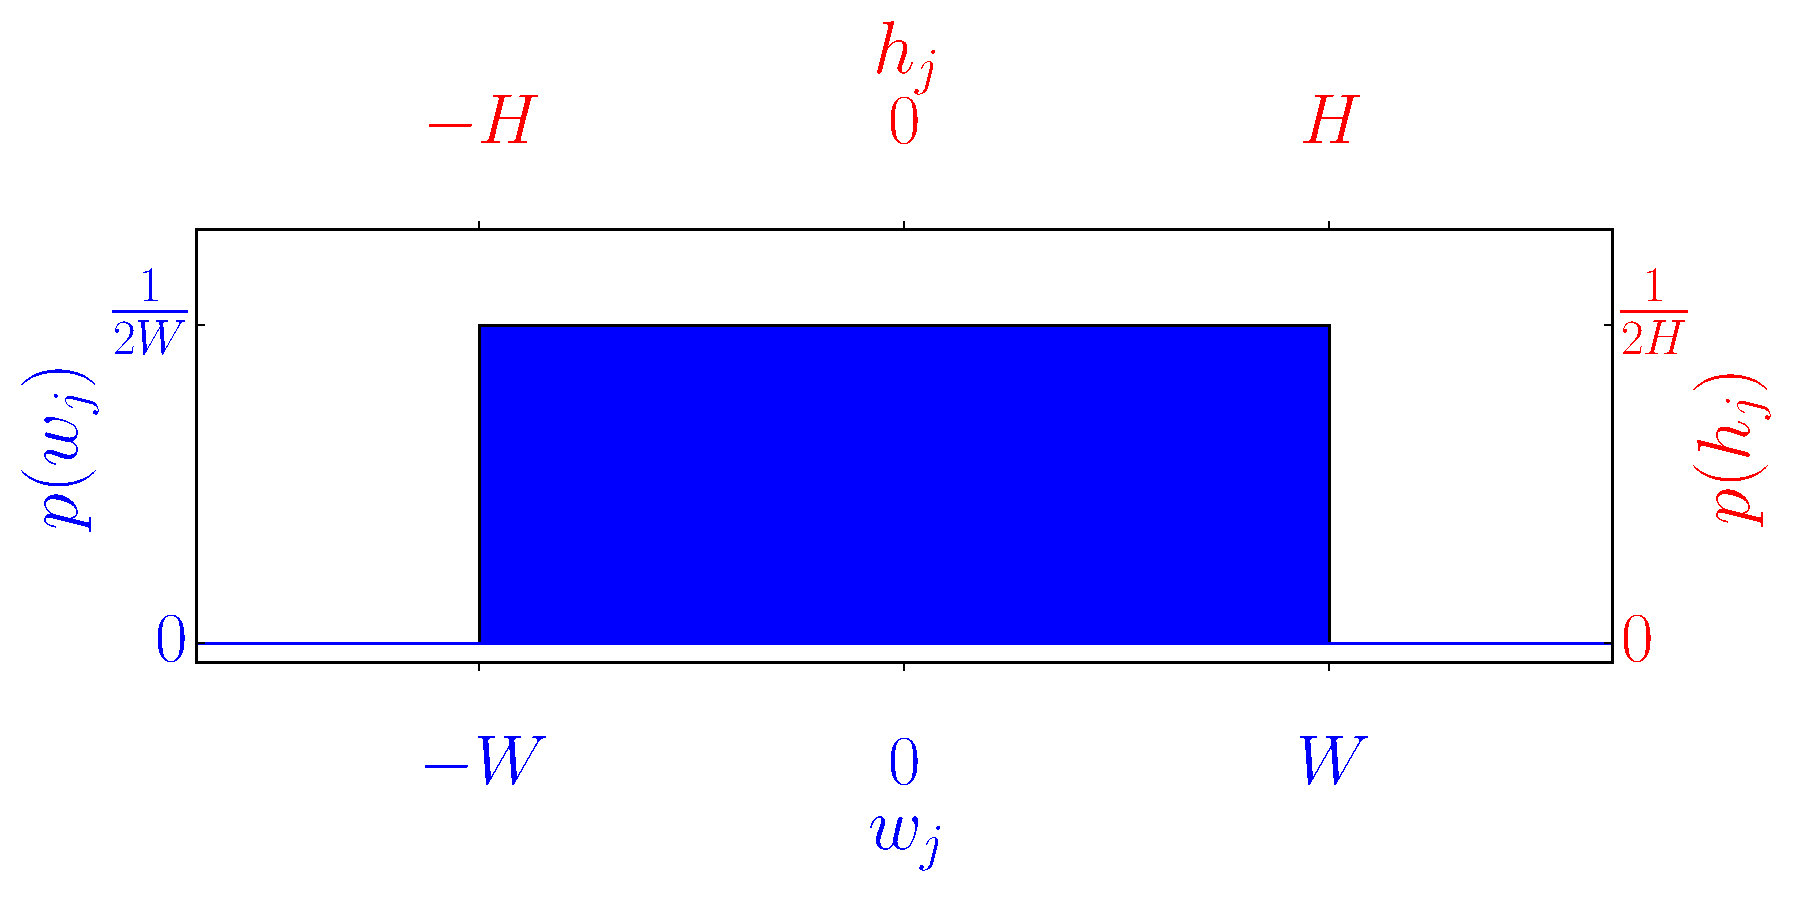
\includegraphics[width=0.62\textwidth]{prob_dist.pdf}}
\end{figure}
\begin{figure}[H]
\centering{
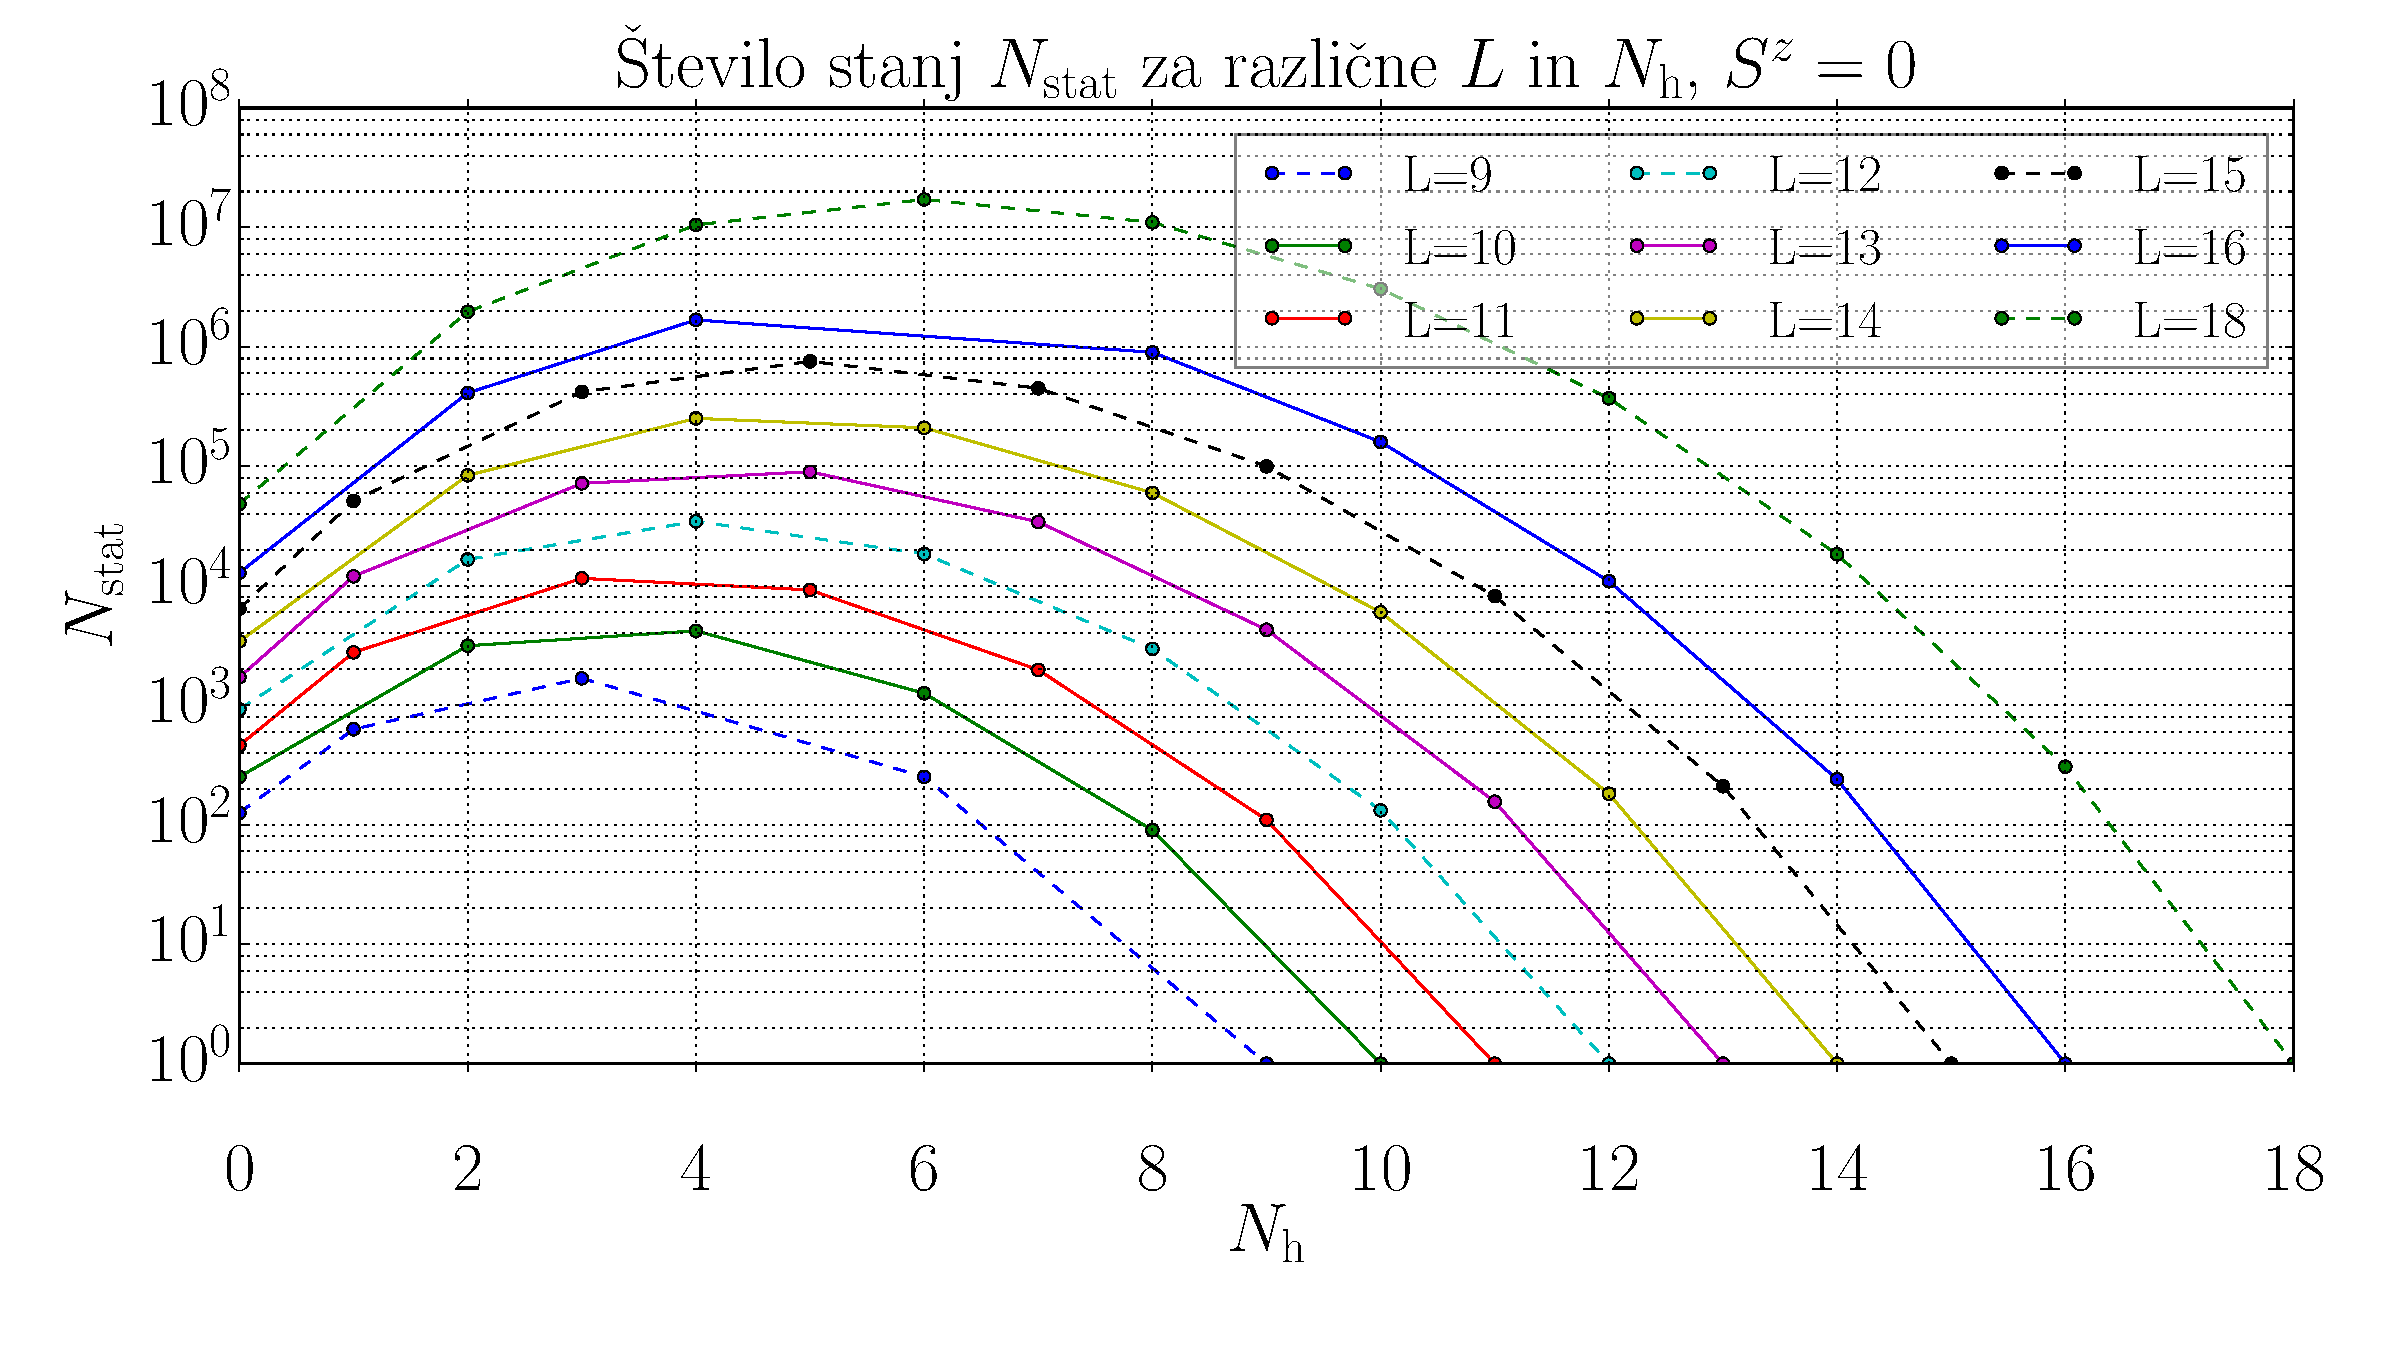
\includegraphics[width=0.8\textwidth]{tJ_num_states.pdf}}
\caption{Odvisnost števila stanj od velikosti sistema in števila dopantov (vrzeli) razkrije, da smo pri študijah s polno diagonalizacijo precej omejeni s številom dostopnih sistemov, ki so nam na voljo, kar precej oteži skalirno analizo, s katero bi radi napovedali obnašanje sistema v termodinamski limiti neskončnega sistema.}
\label{fig:tJ_num_states}
\end{figure}
% \subsection{Preslikava med Hubbardovim modelom in modelom $t$-$J$}
\newpage
\section{Točna diagonalizacija modelskih hamiltonk}
\label{diagonalizacija_metoda}
V Poglavjih~\ref{statisticne_lastnosti} in~\ref{prepletenostna_numericno} predstavljena numerična analiza modela $t$-$J$ temelji na točni diagonalizaciji modelskih hamiltonk, podanih z En.~\eqref{eq:tJ_ham}. Pri dani vrednosti parametrov $t, J, W$ in $H$ hamiltonko najprej diagonaliziramo pri različnih realizacijah nereda. Diagonalizacijo izvedemo s programom, napisanem v programskem jeziku \url{fortran}, pri čemer diagonalizacijo izvedemo s klicem rutine \url{spev} iz Intelove knjižnice \url{MKL}, ki je namenjena diagonalizaciji realnih simetričnih matrik. Izračune izvajamo na gruči \url{LIPS} na odseku F1 na Inštitutu Jožef Stefan. Primer rezultatov diagonalizacije je prikazan na grafih na Slikah~\ref{fig:Eigenstates_spin_hole_disorder_13_1_6.pdf} in~\ref{fig:Eigenstates_spin_hole_disorder_12_4_4.pdf}, in sicer za primera z dopiranjem z eno vrzeljo in s tretjinskim dopiranjem. Grafi na Slikah~\ref{fig:DOS_spin_hole_disorder_13_1_6.pdf} in~\ref{fig:DOS_spin_hole_disorder_12_4_4.pdf} prikazujejo normalizirano gostoto stanj za oba primera.
\vspace{3cm} 	
 \begin{figure}[H]
\centering{
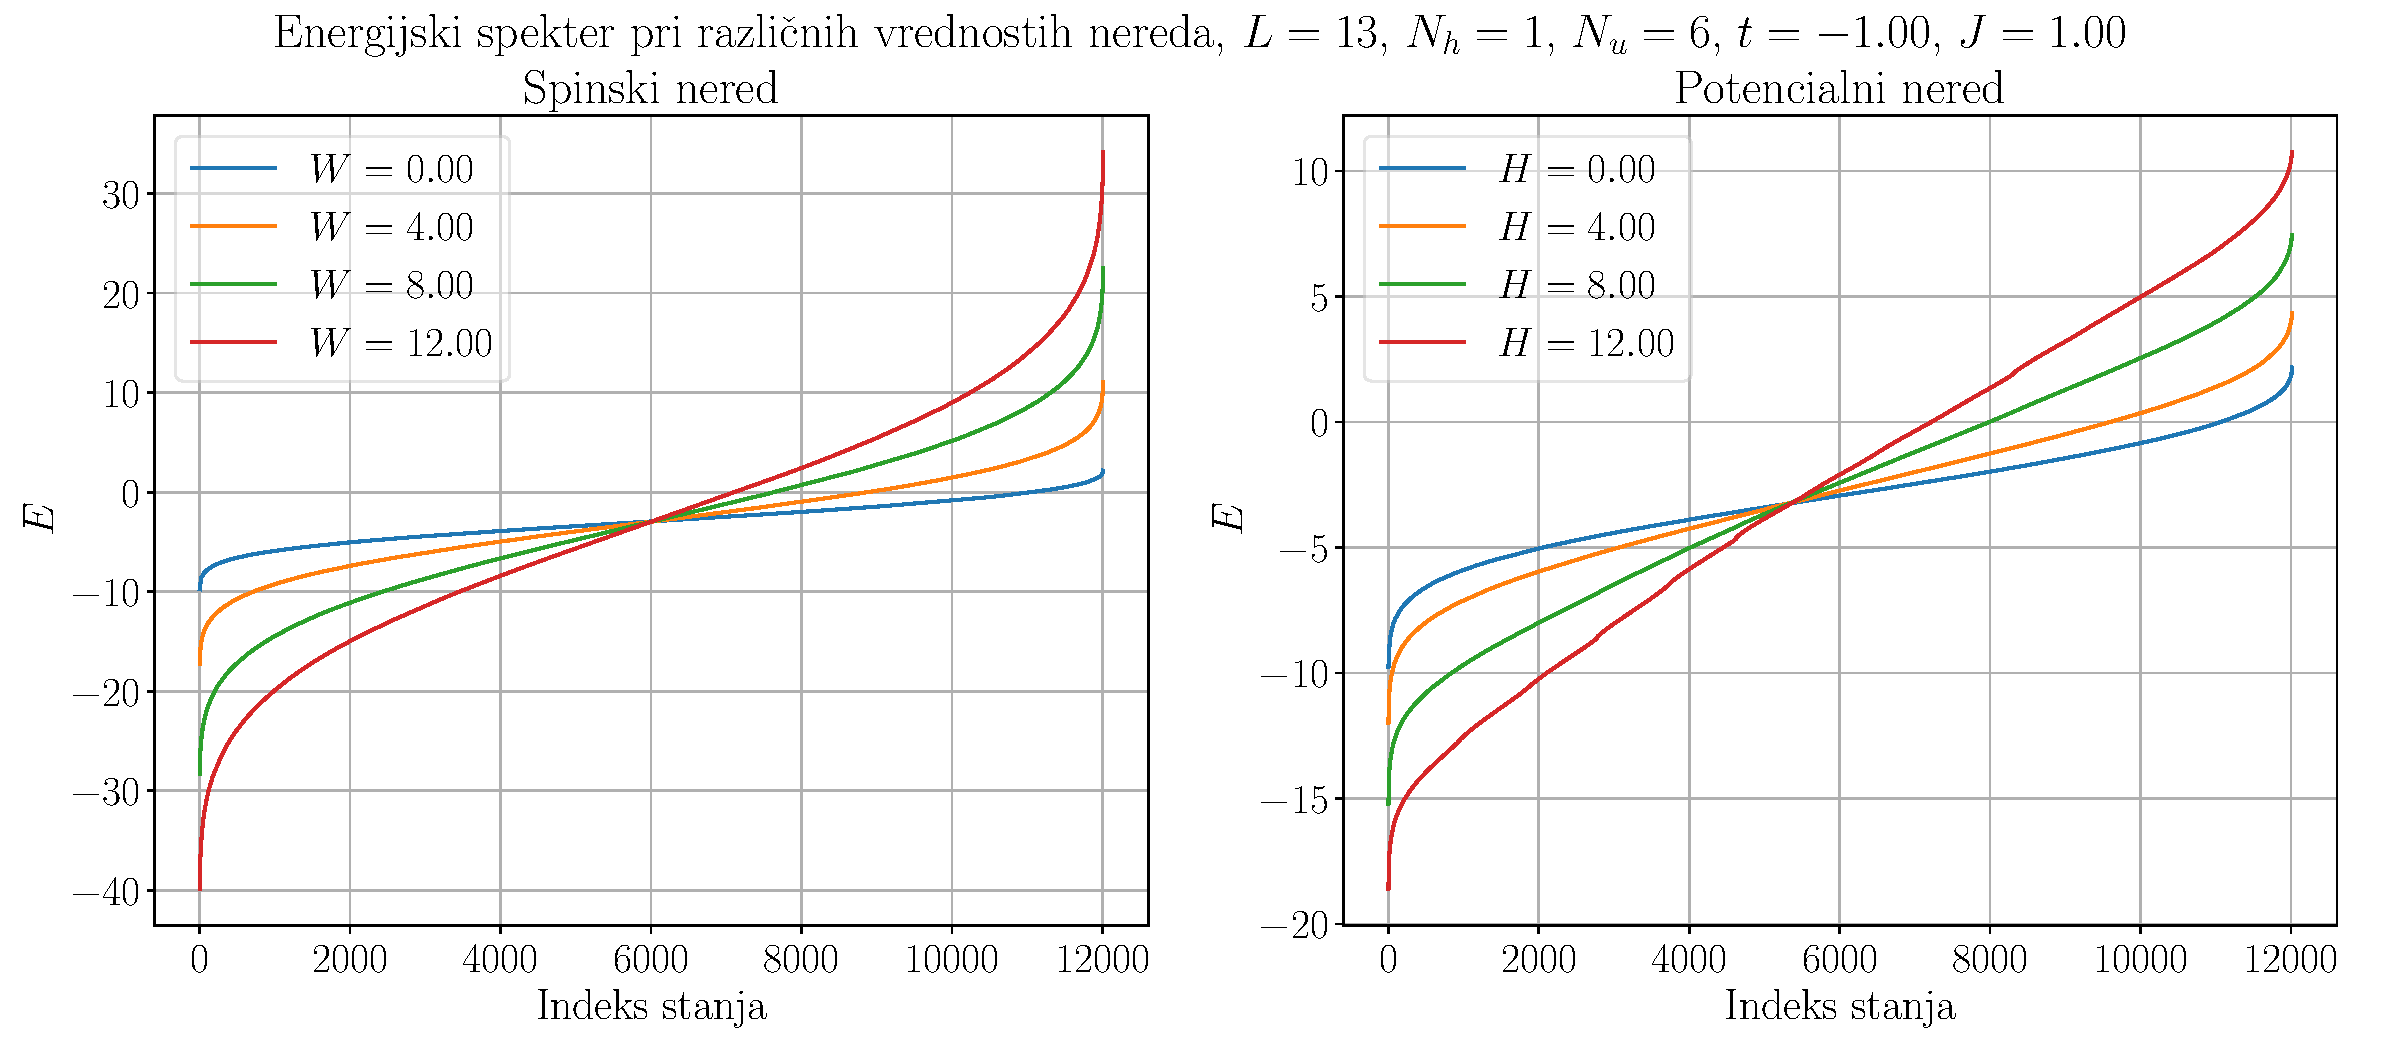
\includegraphics[width=1\textwidth]{Eigenstates_spin_hole_disorder_13_1_6.pdf}}
\caption{Primeri energijskih spektrov pri $L=13, N_h=1, N_u=6.$ Prikazani so rezultati za različne vrednosti parametrov $W$ in $H$, pri čemer so rezultati za spinski nered vsakokrat izračunani s povprečenjem po 100 realizacijah nereda, rezultate za potencialni nered pa s povprečenjem po 600 realizacijah. Pri dopiranju z eno samo vrzeljo opazimo, da je vpliv povečevanja spinskega nereda na spekter znatno večji od vpliva povečevanja potencialnega nereda. Razlog povprečenja po večjem številu realizacijah spinskega nereda je naveden v komentarju k Sliki~\ref{fig:DOS_spin_hole_disorder_13_1_6.pdf}.  }
\label{fig:Eigenstates_spin_hole_disorder_13_1_6.pdf}
\end{figure}
\newpage
 \begin{figure}[H]
\centering{
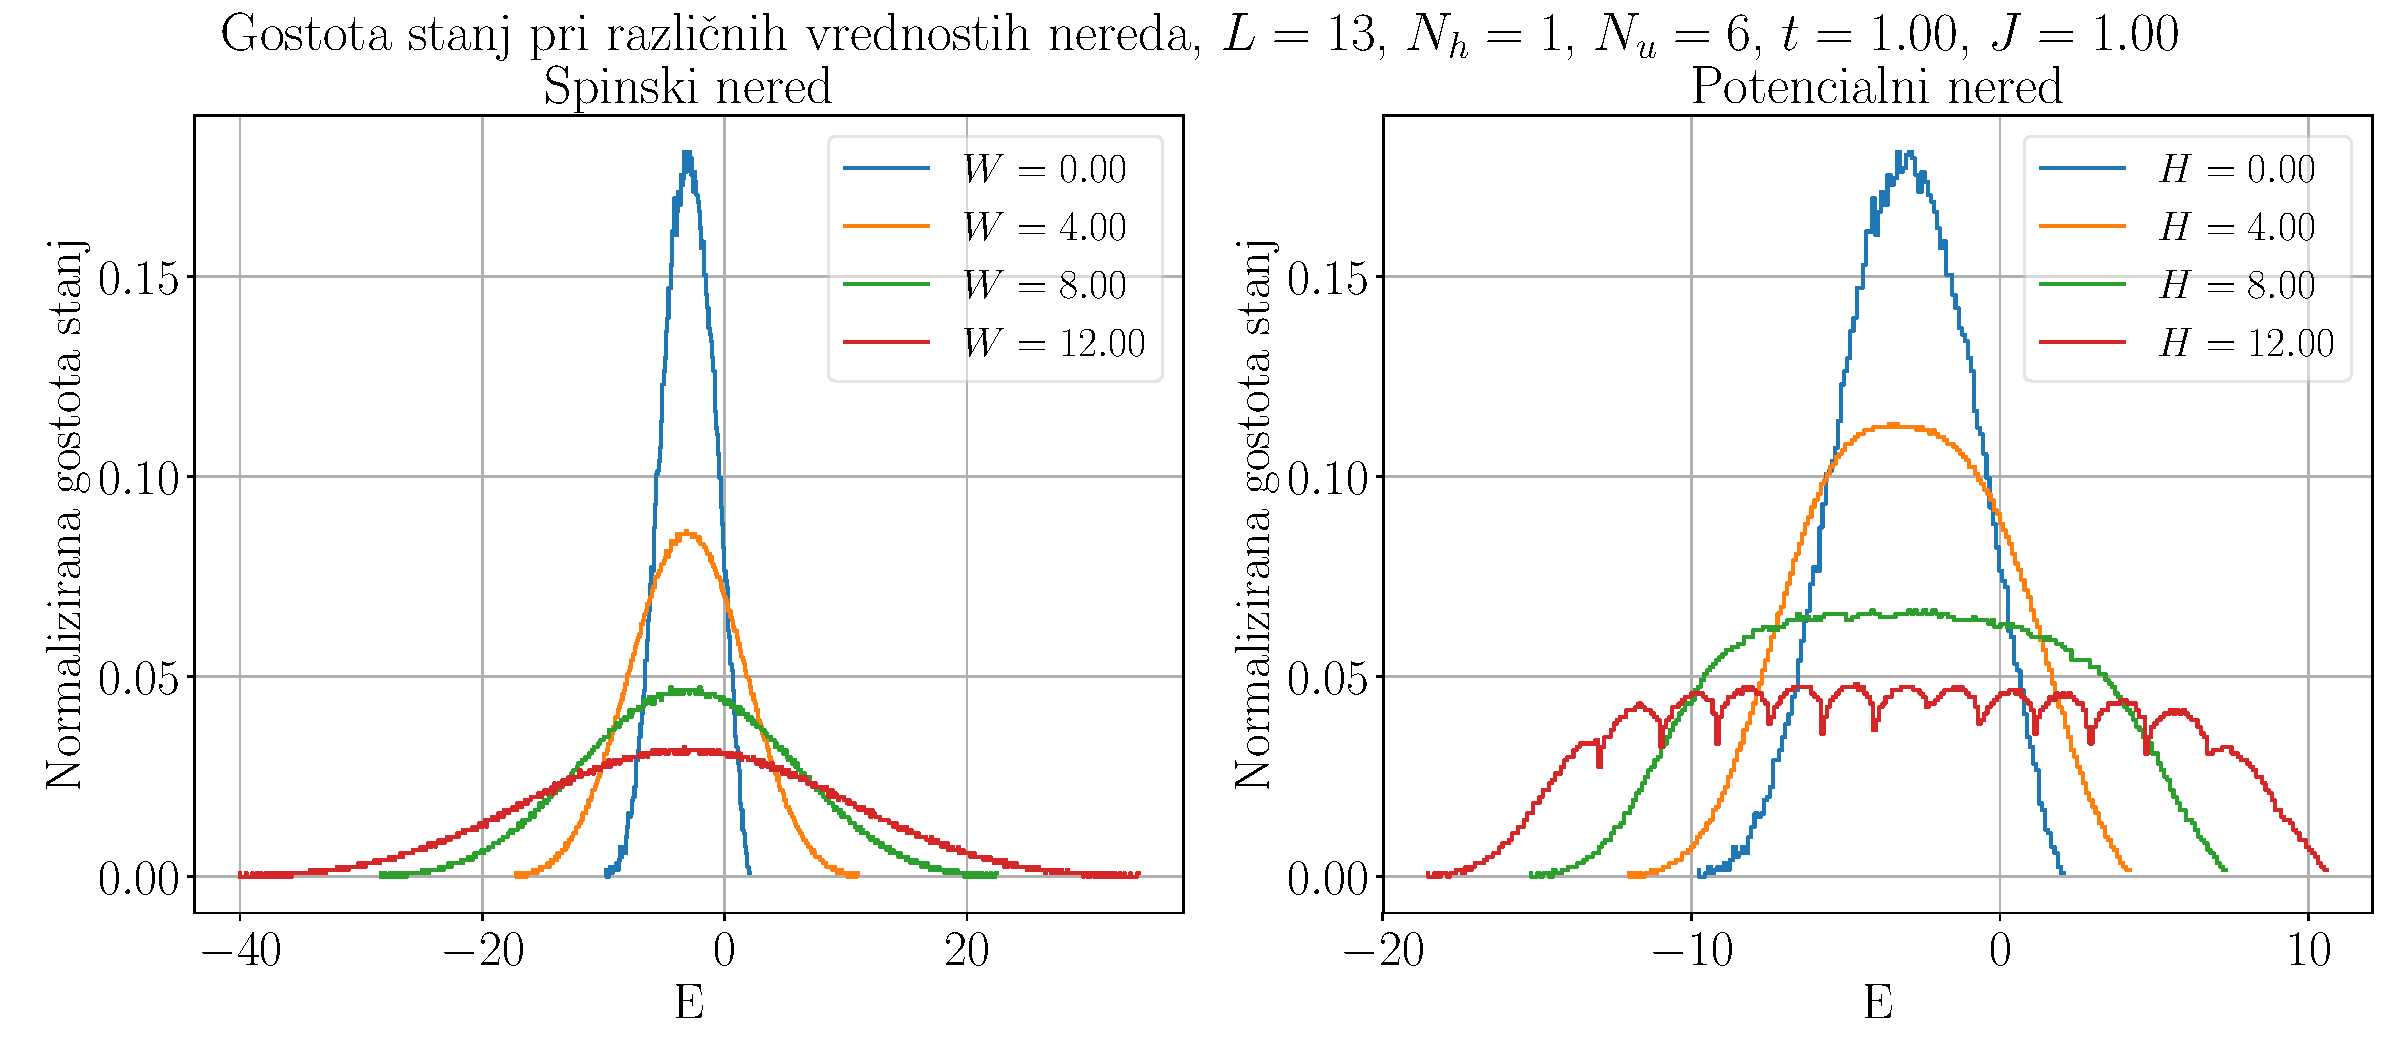
\includegraphics[width=0.9\textwidth]{DOS_spin_hole_disorder_13_1_6.pdf}}
\caption{Normalizirano število stanj na energijski interval za spektre, prikazane na Sliki~\ref{fig:Eigenstates_spin_hole_disorder_13_1_6.pdf}. V primeru spinskega nereda ima gostota stanj vselej izrazit vrh na sredini spektra. Oscilacije v primeru velikega potencialnega nereda $H=12$ so najverjetneje posledica prisotnosti zgolj ene vrzeli. Slednjo lahko na $L$ mest razporedimo na $L$ načinov, toliko je tudi različnih matričnih elementov v (diagonalnem) naključnem potencialnem členu $H_u$. Pri velikih parametrih nereda $H$, kot je na naši energijski skali npr. $H=12$, postane prispevek člena $H_u$ v hamiltonki dominanten, zato opazimo oscilacije gostote stanj. Lokalni minimumi slednje ločijo ravno $L=13$ različnih sektorjev. Grafe za spinski nered smo izračunali s povprečenjem po 100 realizacijah nereda, grafe za potencialni nered pa smo preizkušali povprečenja z med 100 in 600 realizacijami. Kvalitativno se ne zdi, da bi večje povprečenje bistveno spremenilo obliko krivulje, zato je na grafu prikazan le primer povprečenja po 600 vzorcih.}
\label{fig:DOS_spin_hole_disorder_13_1_6.pdf}
\end{figure}
 \begin{figure}[H]
\centering{
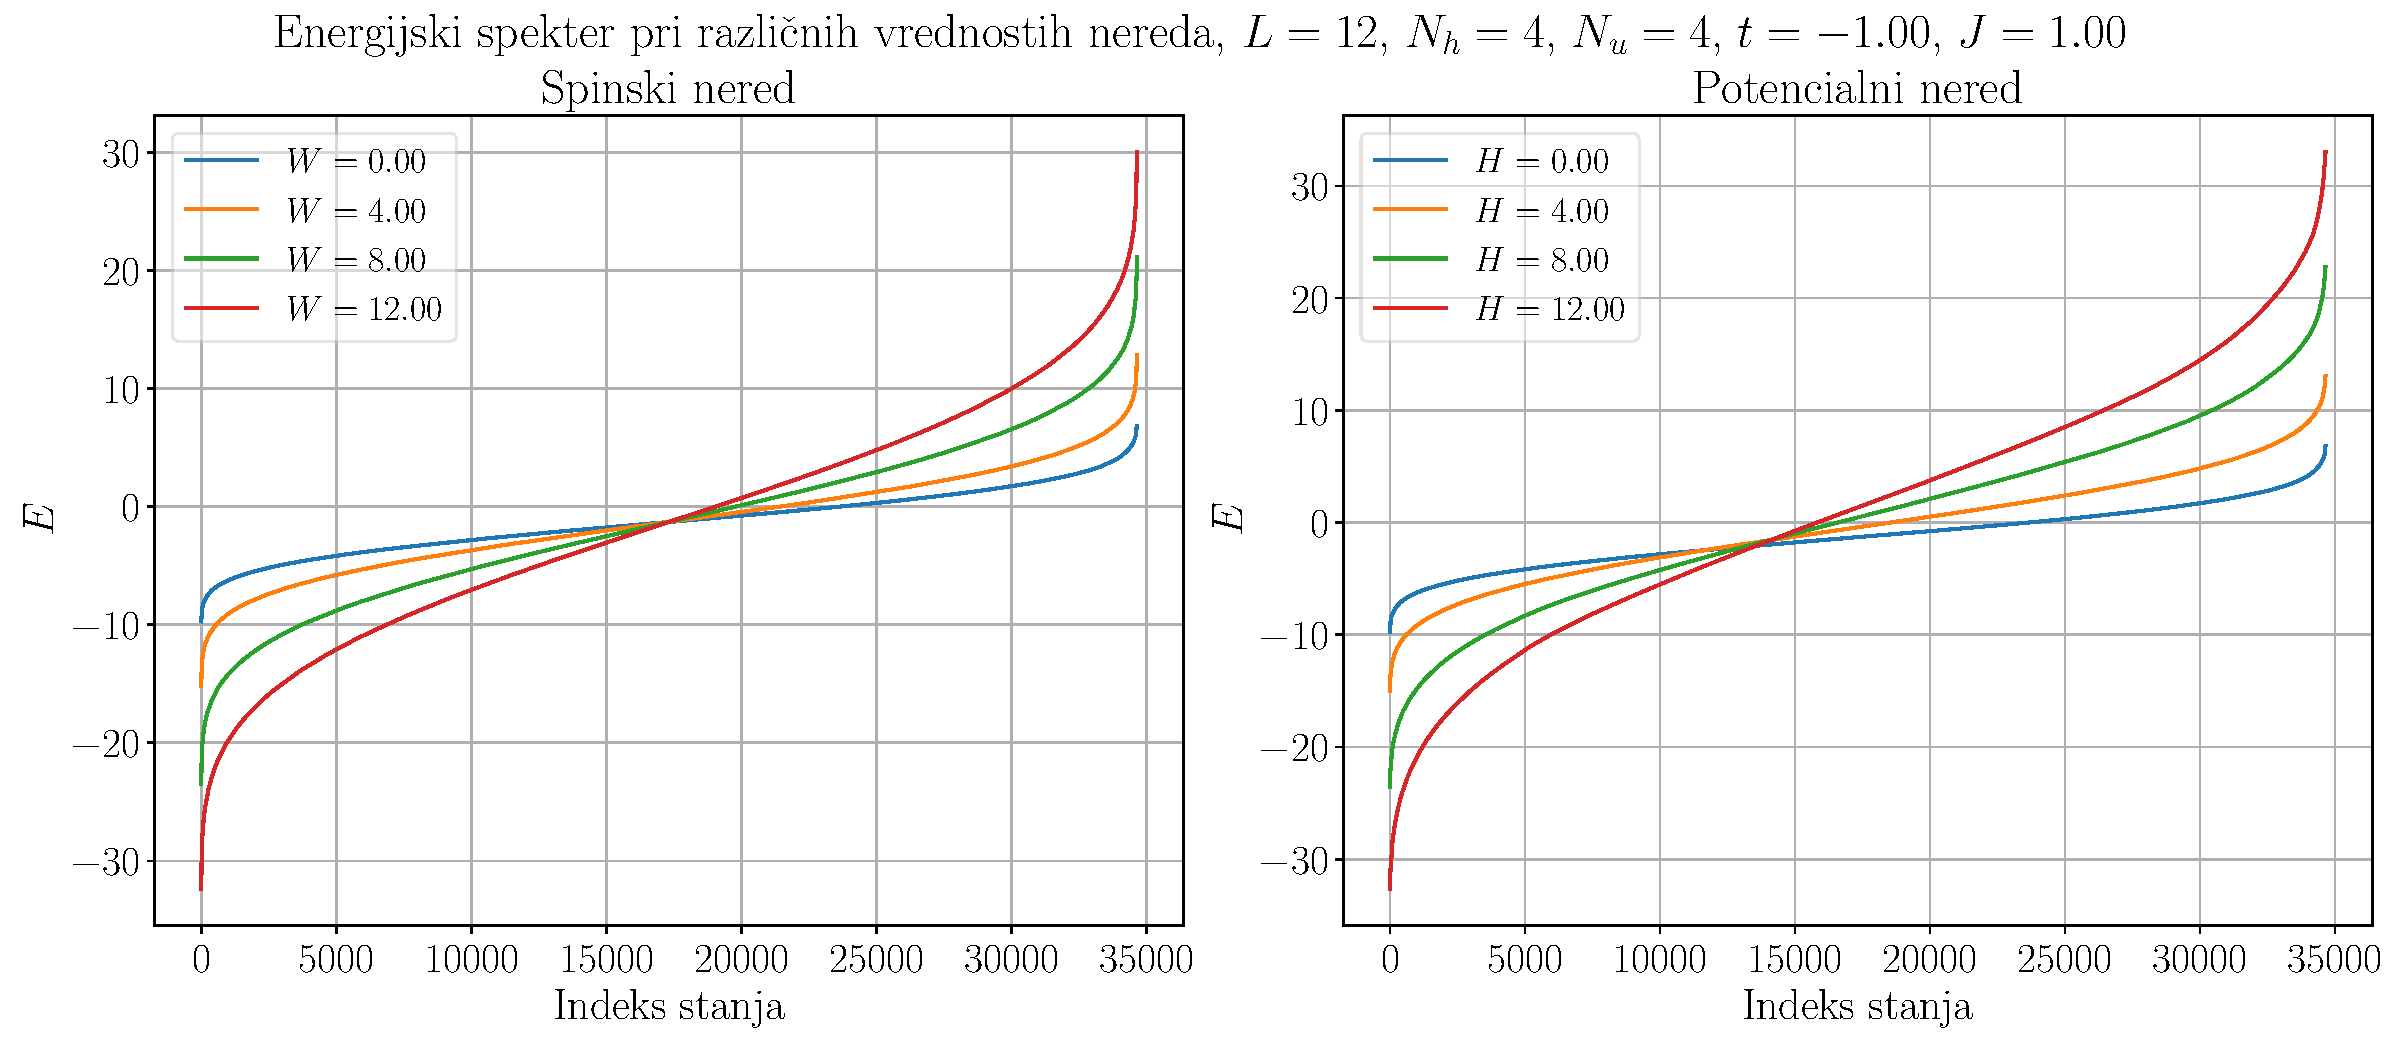
\includegraphics[width=1\textwidth]{Eigenstates_spin_hole_disorder_12_4_4.pdf}}
\caption{Energijski spektri v primeru spinskega in potencialnega nereda za tretjinsko dopiranje na sistemu z $N_\mathrm{stat}=34650$ stanji. V tem primeru sta vpliva spinskega in potencialnega nereda na širino spektra dokaj podobna. Energijsko skalo prispevka spinskega nereda ocenimo kot $(L-N_h)\cdot \frac{W}{2}$, kjer s faktorjem $\frac{1}{2}$ upoštevamo velikost spina v izrazu za zeemansko sklopitev spinov z magnetnim poljem. Energijsko skalo potencialnega nereda podaja vrednost $N_h\cdot H$. Zaradi razmeroma velikih sistemov smo povprečenje izvedli po $50$ naključnih vzorcih za vsak tip nereda.   }
\label{fig:Eigenstates_spin_hole_disorder_12_4_4.pdf}
\end{figure}
 \begin{figure}[H]
\centering{
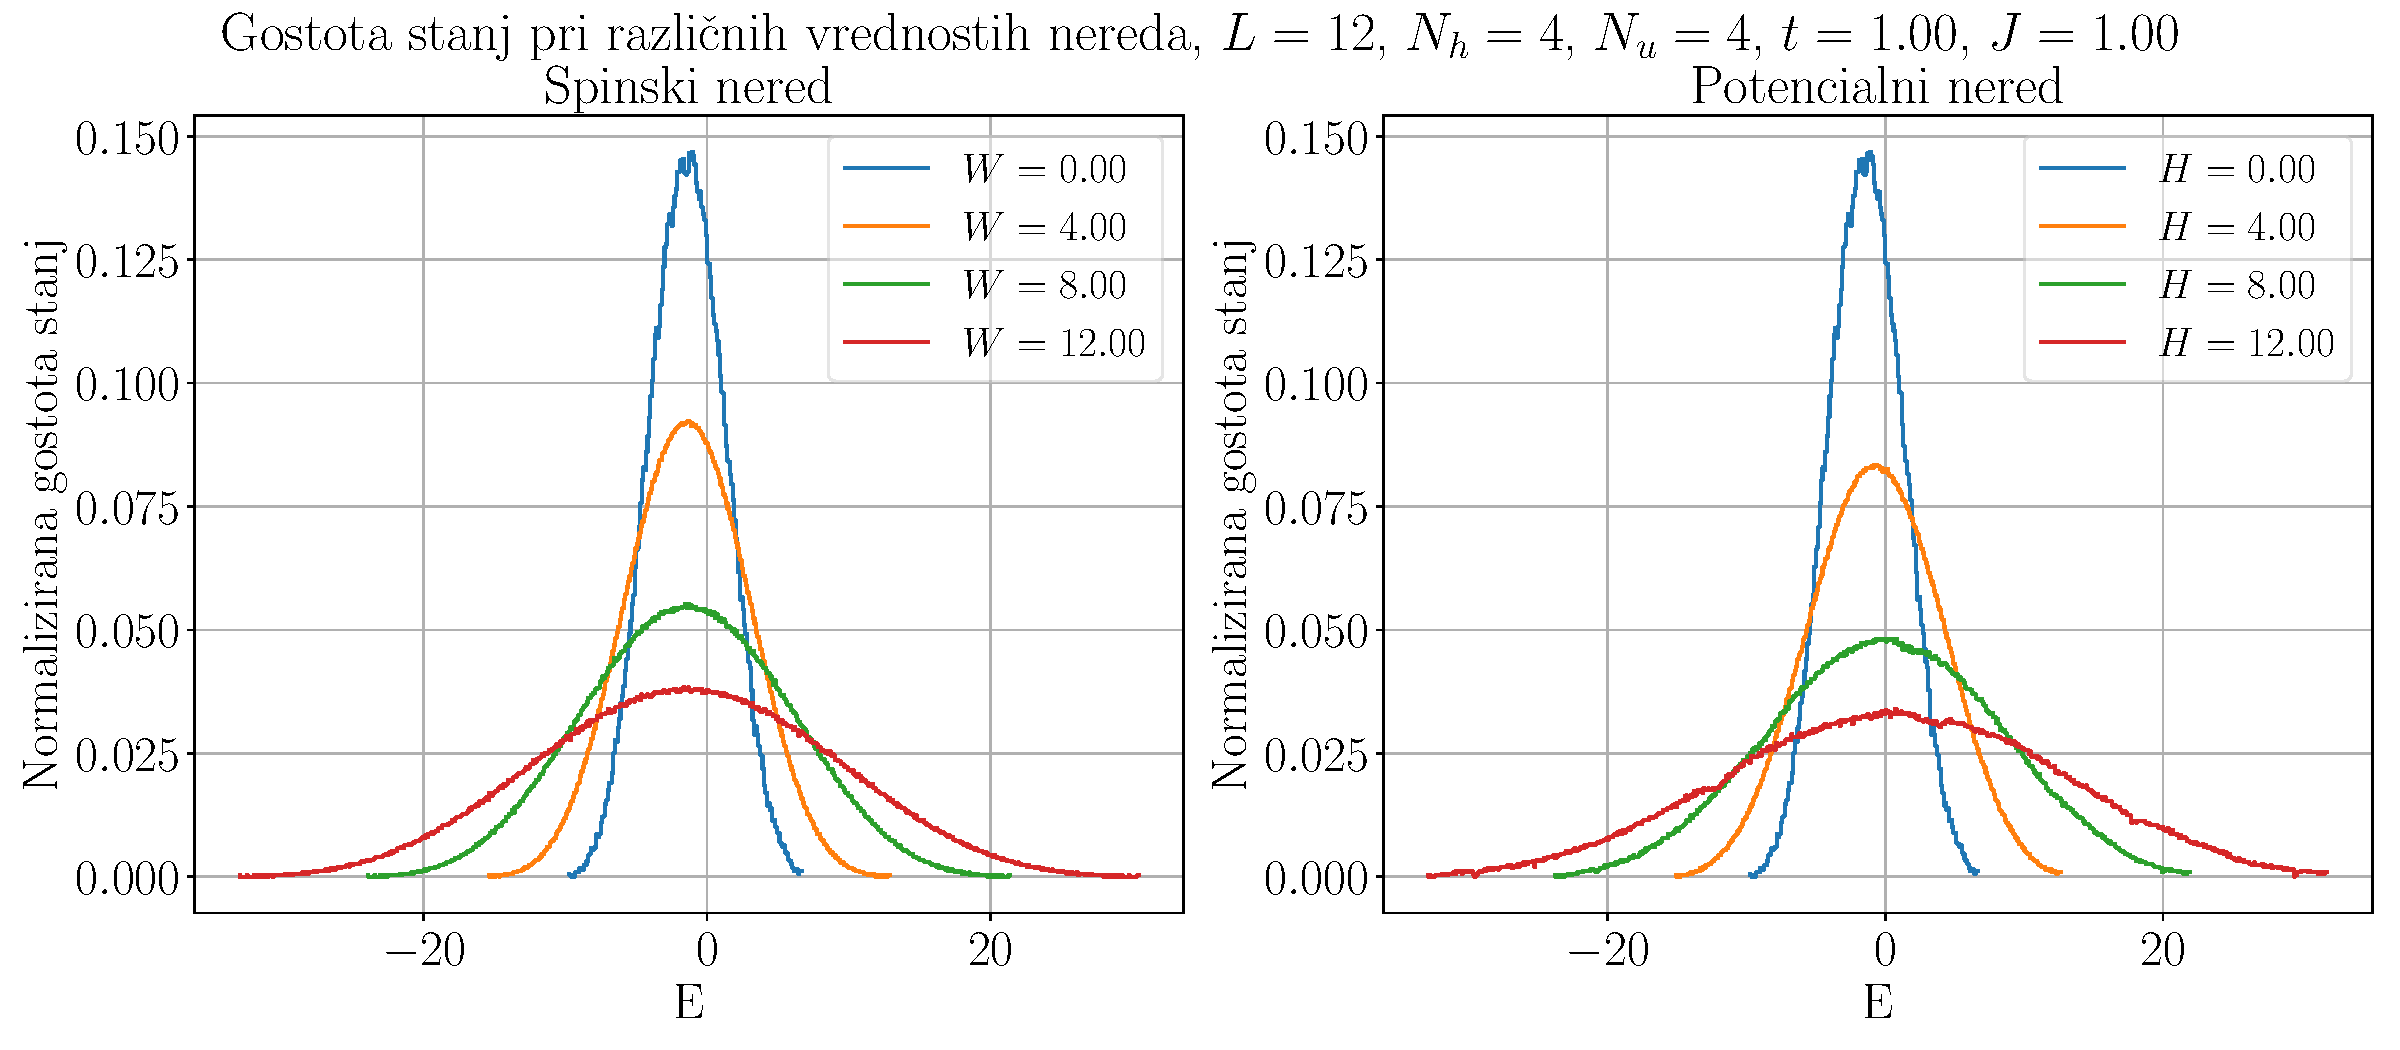
\includegraphics[width=1\textwidth]{DOS_spin_hole_disorder_12_4_4.pdf}}
\caption{Gostota stanj za primer s tretjinskim dopiranjem in spinskim oziroma potencialnim neredom. Oscilacij gostote stanj v primeru potencialnega nereda tokrat ne opazimo. }
\label{fig:DOS_spin_hole_disorder_12_4_4.pdf}
\end{figure}

\chapter{Statistične lastnosti hamiltonskih spektrov}
\label{statisticne_lastnosti}
\section{Statistika sosednjih energijskih nivojev}
\label{statistika_sosednjih_nivojev}
Za presojo ergodičnosti oziroma večdelčne lokaliziranosti sistema analiziramo statistiko energijskih spektrov modelske hamiltonke pri različnih vrednostih parametrov nereda $W$ in $H$. Pri tem se zanašamo na spoznanja teorije naključnih matrik~\cite{mehta2004random} (ang.~\emph{random matrix theory}, v nadaljevanju RMT), ki temelji na pionirskem delu Eugenea Wignerja in Freemana J. Dysona, ki sta razvila teoretični model za opis energijskih spektrov kompleksnih atomskih jeder. Njuna ideja temelji na predpostavki, da je točna napoved energijskih nivojev in njim pripadajočih lastnih stanj v kompleksnih sistemih, kot so jedra težkih elementov, tako rekoč brezupna naloga. Namesto točnega izračuna je zato smiselneje preučevati statistične lastnosti spektrov. Druga ključna opazka je, da imajo modelske hamiltonke kompleksnih sistemov v generičnih bazah strukturo, ki je močno podobna strukturi naključnih matrik. Slednje velja v primeru, ko matrične elemente opazujemo v dovolj ozkem energijskem oknu, v katerem je gostota stanj približno konstantna. Analiza spektralnih lastnosti naključnih matrik tako lahko omogoči vpogled tudi v spektralne lastnosti hamiltonk kompleksnih sistemov, v kolikor zagotovimo, da naključne matrike pripadajo simetrijskemu razredu preučevane modelske hamiltonke. \\\\
 Generičnost baze pomeni splošno izbiro baze, ki ni posebej `prikrojena' za potrebe našega problema. V poglavju~\ref{modelimetode} predstavljena baza zasedenosti stanj ali baza lastnih stanj hamiltonke seveda nista generični bazi, saj ima v njih hamiltonka redko pasovno oziroma diagonalno strukturo, neničelni matrični elementi pa so vse prej kot naključni~\cite{d2016quantum}. Napovedi RMT so kljub temu veljavne, saj predpostavka naključnih matričnih elementov velja za izbiro splošne baze. \\\\
 V naslednjih poglavjih predstavimo Wigner-Dysonovo in Poissonovo statistiko, ki opišeta razmik med sosednjimi energijskimi nivoji v ergodičnem in MBL ali integrabilnem sistemu. Razmik med sosednjimi energijskimi nivoji je definiran kot 
 \begin{equation}\label{eq:razmik}
 s_n=E_{n+1}-E_n,
 \end{equation}
 kjer je $E_n$ $n$-ti energijski nivo. \\\\
 Poleg statistike odmikov med sosednjimi nivoji 
 preučujemo tudi statistiko razmerij odmikov med sosednjimi energijskimi nivoji, ki sta jo v članku iz leta 2007~\cite{PhysRevB.75.155111} prva uvedla Oganesyan in Huse:
 \begin{equation}\label{eq:oganesyan_huse}
 \tilde{r}_n=\frac{\min\left(s_n,s_{n-1}\right)}{\max\left(s_n,s_{n-1}\right)}, \hspace{5mm} r_n=\frac{s_n}{s_{n-1}}.
 \end{equation}
 V praksi ergodičnost oziroma večdelčno lokaliziranost sistema presojamo na podlagi povprečne vrednosti $\langle \tilde{r}\rangle$, za katero v obeh režimih obstajata dobro določeni limitni vrednosti~\cite{Atas_Distribution_PhysRevLett.110.084101}. Statistika razmerij odmikov $\tilde{r}_n$ je v primerjavi s statistiko razmikov med nivoji $s_n$ za obravnavo prikladnejša, saj pred izračunom ni treba izvesti \emph{razgrnjenja} spektra (ang.~\emph{spectral unfolding}), ki ga podrobneje predstavimo v poglavju~\ref{razgrnjenje}.
 % Poleg tega je povprečje $\langle \tilde{r}\rangle$ za vizualizacijo prikladnejša količina kot porazdelitev energijskih nivojev. 
 \subsection{Wigner-Dysonova statistika razmikov med sosednjimi nivoji} 
 V tem poglavju je izpeljana Wigner-Dysonova statistika za razmik med sosednjimi energijskimi nivoji v naključnih matrikah. Pri izpeljavi sledimo preglednemu članku, navedenem v Ref.~\cite{d2016quantum}.
 Osnovno idejo RMT lahko predstavimo z analizo hamiltonke velikosti $2\times2$, v kateri matrične elemente izžrebamo v skladu z Gaussovo verjetnostno porazdelitvijo z ničelnim povprečjem in varianco $\sigma$.  Pri tem upoštevamo še simetrije našega problema:
 \begin{equation}\label{eq:rnd_ham}
 \hat{H}=
 \begin{bmatrix}
 \varepsilon_1 & \frac{V}{\sqrt{2}} \\
 \frac{V^*}{\sqrt{2}} & \varepsilon_2
 \end{bmatrix}
 \end{equation}
 Če velja simetrija na obrat časa, $V=V^*$, lahko hamiltonko zapišemo kot realno matriko. Slednje drži tudi v primeru hamiltonke, podane z En. \eqref{eq:tJ_ham}. Diagonalizacija naključne $2\times2$ hamiltonke je enostavna, lastni energiji sta
 \begin{equation}
 E_{1,2}=\frac{\varepsilon_1+\varepsilon_2}{2}\pm \frac{1}{2}\sqrt{\left(\varepsilon_1 +\varepsilon_2\right)^2 + 2V^2}
 \end{equation}
 Od tod lahko izračunamo statistiko razmikov med energijskimi nivoji, $P(E_1-E_2=s)\equiv P(s),$
\begin{equation}
 P(s)=\frac{1}{\left(2\pi\right)^{3/2}\sigma^3}\int \dd\varepsilon_1\int\dd\varepsilon_2\int \dd V \delta\left(\sqrt{\left(\varepsilon_1 +\varepsilon_2\right)^2 + 2V^2}-s\right)\exp\left( -\frac{\varepsilon_1^2+\varepsilon_2^2+V^2}{2\sigma^2}\right)
 \end{equation}
 Z zamenjavo spremenljivk, $\varepsilon_2=-\varepsilon_1+\sqrt{2}\xi$ in integracijo po $\varepsilon_1$ dobimo 
 \begin{equation}
 P(s)=\frac{1}{2\pi\sigma^2}\int\int\dd\xi\dd V\delta\left(\sqrt{2\xi^2+2V^2}-s\right)\exp\left(-\frac{\xi^2+V^2}{2\sigma^2}\right)
 \end{equation}
 Z uvedbo cilindričnih koordinat, $V=r\cos(x)$, $\xi=r\sin(x),$ dobimo 
 \begin{equation}\label{eq:wigner_surmise}
 P(s)=\frac{s}{2\sigma^2}\exp\left(-\frac{s^2}{4\sigma^2} \right)
\end{equation}
 Nazadnje porazdelitev še normirano in povprečni razmik med nivoji $\bar{s}$ postavimo na vrednost 1, pa dobimo za realne simetrične naključne matrike \emph{Wigner-Dysonovo} statistiko za razmik med energijskimi nivoji: 
 \begin{equation}\label{eq:wigner-dyson}
 P_\mathrm{WD}(s)=\frac{\pi s}{2}\exp\left(-\frac{\pi}{4}s^2\right)
 \end{equation}
 Zgornja statistika izkazuje dve splošni generični lastnosti, značilni za nivojske statistike kvantnih kaotičnih sistemov. V limiti $s\to 0$ je verjetnost za ničeln razmik med nivoji ničelna, kar kaže na odboj med nivoji (ang.~\emph{level repulsion}). Kot bomo videli nekoliko kasneje, je to bistveno drugače od nivojskih statistik v integrabilnem ali MBL primeru. Za velike razmike $s$ verjetnost $P_\mathrm{WD}(s)$ pada kot gaussovska porazdelitev. Lastnosti statistike so bile sprva izpeljane za kvantne sisteme s klasičnim kaotičnim analogom, a se je kasneje izkazalo, da veljajo tudi za sisteme brez omenjene analogije.\\\\
 Izraz \eqref{eq:wigner_surmise} je eksakten za hamiltonke velikosti $2\times2$, izkaže pa se~\cite{abanin2018ergodicity}~\cite{Atas_Distribution_PhysRevLett.110.084101}, da je ujemanje dobro tudi za višjedimezionalne hamiltonke. V tem primeru definiramo ansambel naključnih matrik, ki jih žrebamo v skladu z naključno Gaussovsko porazdelitvijo kot
 \begin{equation}
 P_\mathrm{GOE}(\hat{H})\propto \exp\left(-\frac{1}{2a^2}\Tr\left(\hat{H}^2\right) \right) \equiv \exp\left(-\frac{1}{2a^2}\sum\limits_{ij}H_{ij}H_{ji} \right)
 \end{equation}
 Tako definiran ansambel matrik se imenuje gaussovski ortogonalni ansambel (GOE), z zgornjo definicijo pa zadostimo zahtevi po invariantnosti ansambla na vsakršne ortogonalne transformacije, saj je porazdelitev odvisna zgolj od sledi kvadrata posamezne hamiltonke, kar je po definiciji invariantna količina. Hkrati je porazdelitev gaussovska, saj je sled vsota kvadratov naključno porazdeljenih matričnih elementov in kot takšna zadošča centralnemu limitnemu izreku. \\\\Izpeljava natančnih izrazov za nivojske statistike hamiltonk iz GOE ni predmet te magistrske naloge, v splošnem zanje zaključena analitična oblika niti ne obstaja. Podrobnejša analiza je navedena v članku v Ref.~\cite{Atas_Distribution_PhysRevLett.110.084101}, tu bomo za presojo uporabljali rezultat, podan z En. \eqref{eq:wigner_surmise}, ki dobro popiše tudi večdimenzionalne primere. 
 \subsection{Poissonova statistika razmikov med sosednjimi nivoji}
 V predhodnem podpoglavju smo obravnavali nivojsko statistiko v kvantnokaotičnih sistemih, v katerih so razmiki med sosednjimi energijskimi nivoji porazdeljeni v skladu z Wigner-Dysonovo statistiko. Porazdelitev za kvantne integrabilne sisteme sta prva obravnavala Berry in Tabor v članku iz leta 1977~\cite{berry1977level}. Za potrebe razjasnitve pojmov, ki nastopajo v magistrski nalogi, so tu navedeni le ključni rezultati. \\\\
 Med enostavnejše primere neergodičnega sistema sodi veriga neodvisnih kvantnih harmonskih oscilatorjev z nesoizmerljivimi (ang.~\emph{incommensurate}) frekvencami. V odsotnosti medsebojne sklopitve lahko vsakega izmed oscilatorjev diagonaliziramo neodvisno od preostalih, skupno energijo pa dobimo s seštevanjem enooscilatorskih energij kot 
 $$
 E=\sum_j n_j\omega_j,
 $$ 
 kjer je $j$ lastna frekvenca, $n_j$ pa zasedbeno število $j$-tega oscilatorja. Za velike vrednosti $E$ dobimo podobne vrednosti energije za različne nabore zasedbenih števil $\{n_j\}$, zato lahko energijske nivoje obravnavamo kot nekorelirana naključna števila. V tem primeru je verjetnost, da se na energijskem intervalu dolžine $\delta E$ nahaja $m$ energijskih nivojev, enaka Poissonovi porazdelitvi 
 \begin{equation}
 P_m=\frac{\lambda^m}{m!}\exp\left(-\lambda \delta E\right),
 \end{equation}
 kjer je $\lambda$ enaka inverznemu povprečnemu razmiku med nivoji v spektru. Porazdelitev razmikov med nivoji tako dobimo na enak način kot porazdelitev čakalnih časov med dogodki v Poissonovem procesu:
 \begin{equation}\label{eq:poisson}
 P_\mathrm{Poisson}(s)=P_0=\exp\left(-s\right)
 \end{equation}
 Pri tem smo postavili $\lambda=1$ in vpeljali $s$ kot  $s=\delta E$. V nasprotju z Wigner-Dysonovo porazdelitvijo pri Poissonovi statistiki ni odboja med nivoji, saj ima porazdelitev vrh pri $s=0$. V integrabilnih sistemih je slednje posledica ohranjenih količin. Podobno je v MBL sistemih veljavnost Poissonove statistike posledica uvedbe naključnih členov v modelsko hamiltonko. \\\\
 Splošna izjava, ki povzame vsebino tega podpoglavja, pravi, da izkazujejo kvantni sistemi s klasičnim analogom Poissonovo statistiko razmikov med sosednjimi energijskimi nivoji. Izjava drži tudi v primeru mnogih kvantnih sistemov brez klasične ustreznice, kljub temu pa obstajajo tudi protiprimeri, npr. en delec v harmonskem potencialu. Predpostavka veljavnosti Poissonove statistike je zato danes znana kot \emph{domneva} Berrya in Taborja (ang.~\emph{Berry-Tabor conjecture})~\cite{berry1977level}.\\\\
 Na Sliki \ref{fig:unfolding_demo_three_slo} so prikazani primeri numerično izračunanih nivojskih statistik v ergodičnem, vmesnem in MBL režimu skupaj z Wigner-Dysonovo in Poissonovo statistiko. 
 \subsection{Statistika razmerij odmikov sosednjih nivojev $\tilde{r}$}
 \label{statistika_razmerij_odmikov}
 Po postopku, opisanem v poglavju o numerični implementaciji izračunov, izračunamo povprečno vrednost količine $\tilde{r}$, ki jo podaja En. \eqref{eq:oganesyan_huse}. V ergodičnem primeru mora izračunana vrednost $\langle \tilde{r}\rangle$ čim bolje ustrezati GOE vrednosti, ki znaša:
 \begin{equation}\label{eq:r_GOE}
 \langle \tilde{r}\rangle_\mathrm{GOE}=0.5307
 \end{equation}
 V integrabilnem ali MBL primeru ustreza povprečno razmerje razmikov sosednjih nivojev vrednosti za Poissonovo porazdeljen spekter lastnih vrednosti: 
 \begin{equation}\label{eq:r_poisson}
 \langle \tilde{r}\rangle_\mathrm{Poisson}=0.38629
 \end{equation}
Vrednost $\langle \tilde{r}_\mathrm{GOE}\rangle$ je bila izračunana numerično, medtem ko je napoved $\langle\tilde{r}_\mathrm{Poisson}\rangle$ točna analitična vrednost~\cite{Atas_Distribution_PhysRevLett.110.084101}.
\begin{figure}[H]
\centering{
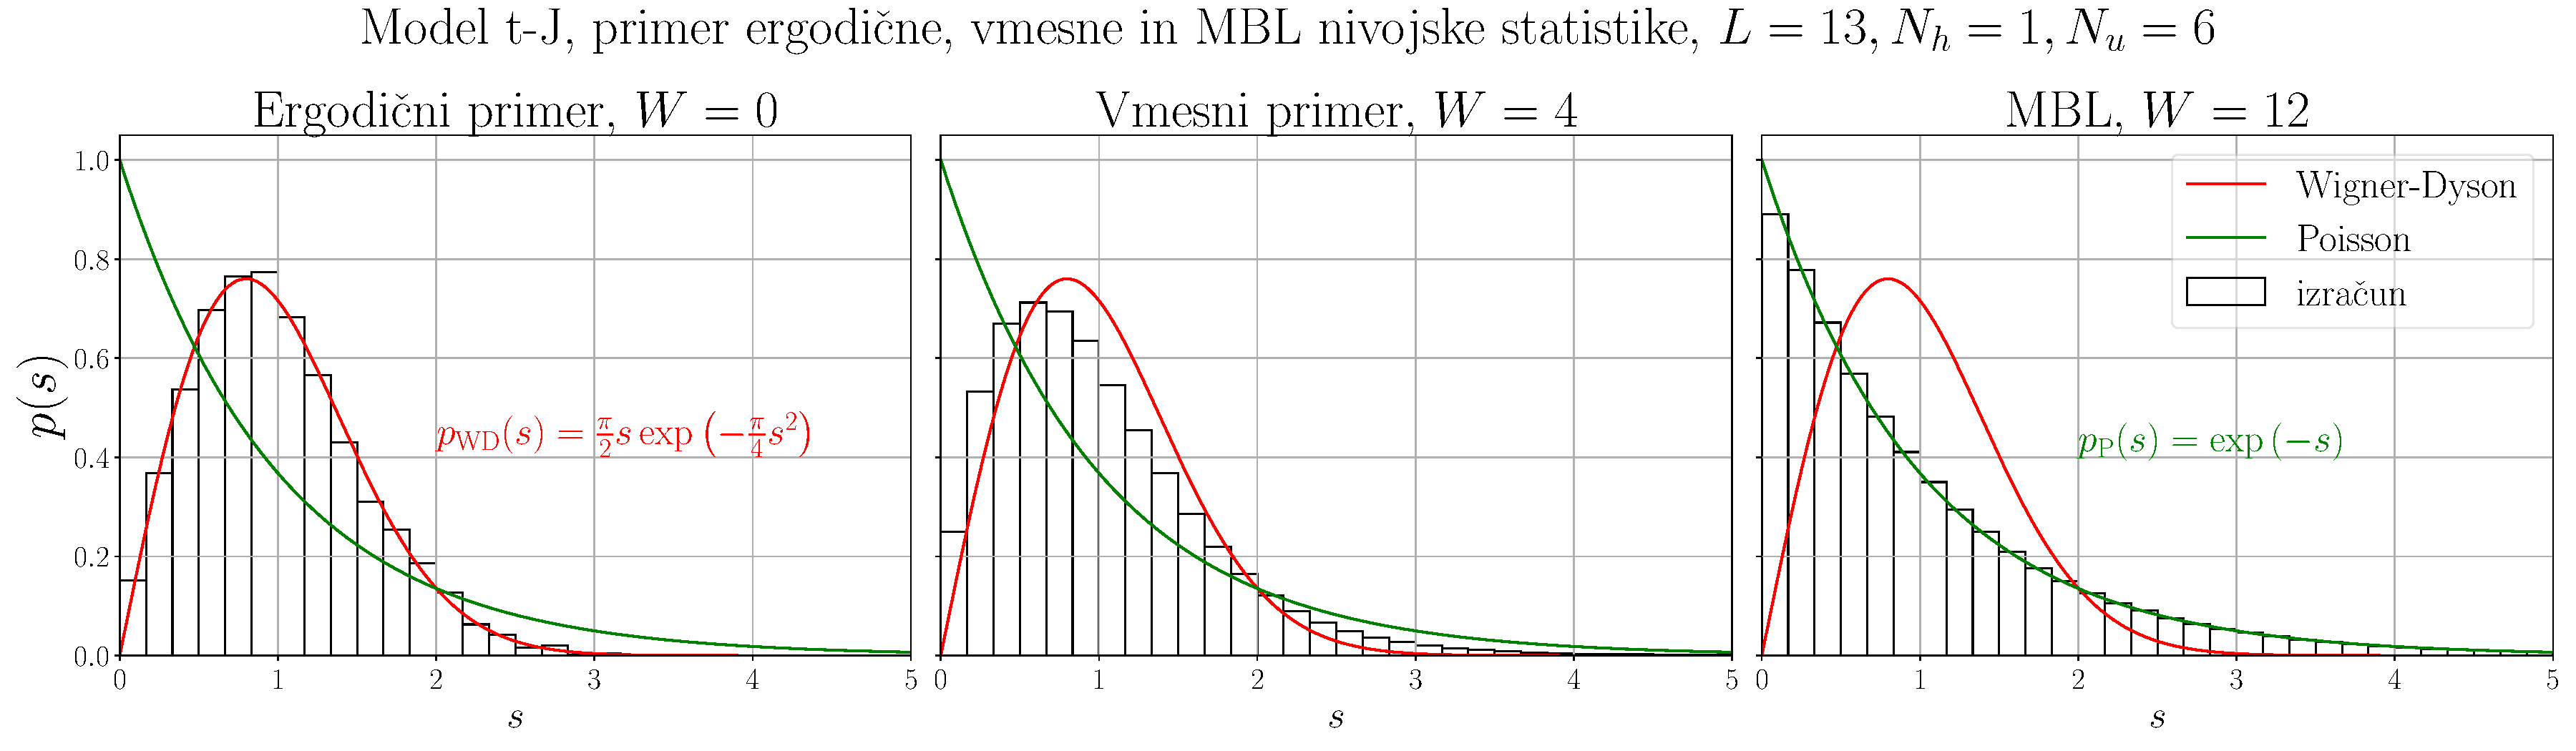
\includegraphics[width=1\textwidth]{unfolding_demo_three_slo.pdf}}
\caption{Numerično izračunana statistika razmikov med sosednjimi energijskimi nivoji za model $t$-$J$, $L=13$, $N_h=1$, $N_u=6$. Uporabili smo vrednosti modelskih parametrov $t=1$ in $J=1,$ ki sta od tu naprej za vse prikazane simulacije enaki. Na podlagi komplementarnih študij časovne dinamike modela~\cite{lemut2017complete} smo izbrali vrednosti parametra spinskega nereda $W$, za katere je obnašanje sistema poznano. Pri $W=0$ je sistem ergodičen, kar je razvidno iz ujemanja numeričnih izračunov s krivuljo Wigner-Dysonove statistike, podobno je pri $W=12$ dobro ujemanje s krivuljo Poissonove statistike. V vmesnem režimu se numerično izračunane vrednosti ne ujemajo z nobeno od teoretičnih napovedi. Pri dani konfiguraciji ima model 12012 stanj, rezultati pa so izračunani s povprečenjem po 100 realizacijah spinskega nereda. Natančne podrobnosti numerične implementacije so podane v naslednjem poglavju.  }
\label{fig:unfolding_demo_three_slo}
\end{figure}
\begin{figure}[H]
\centering{
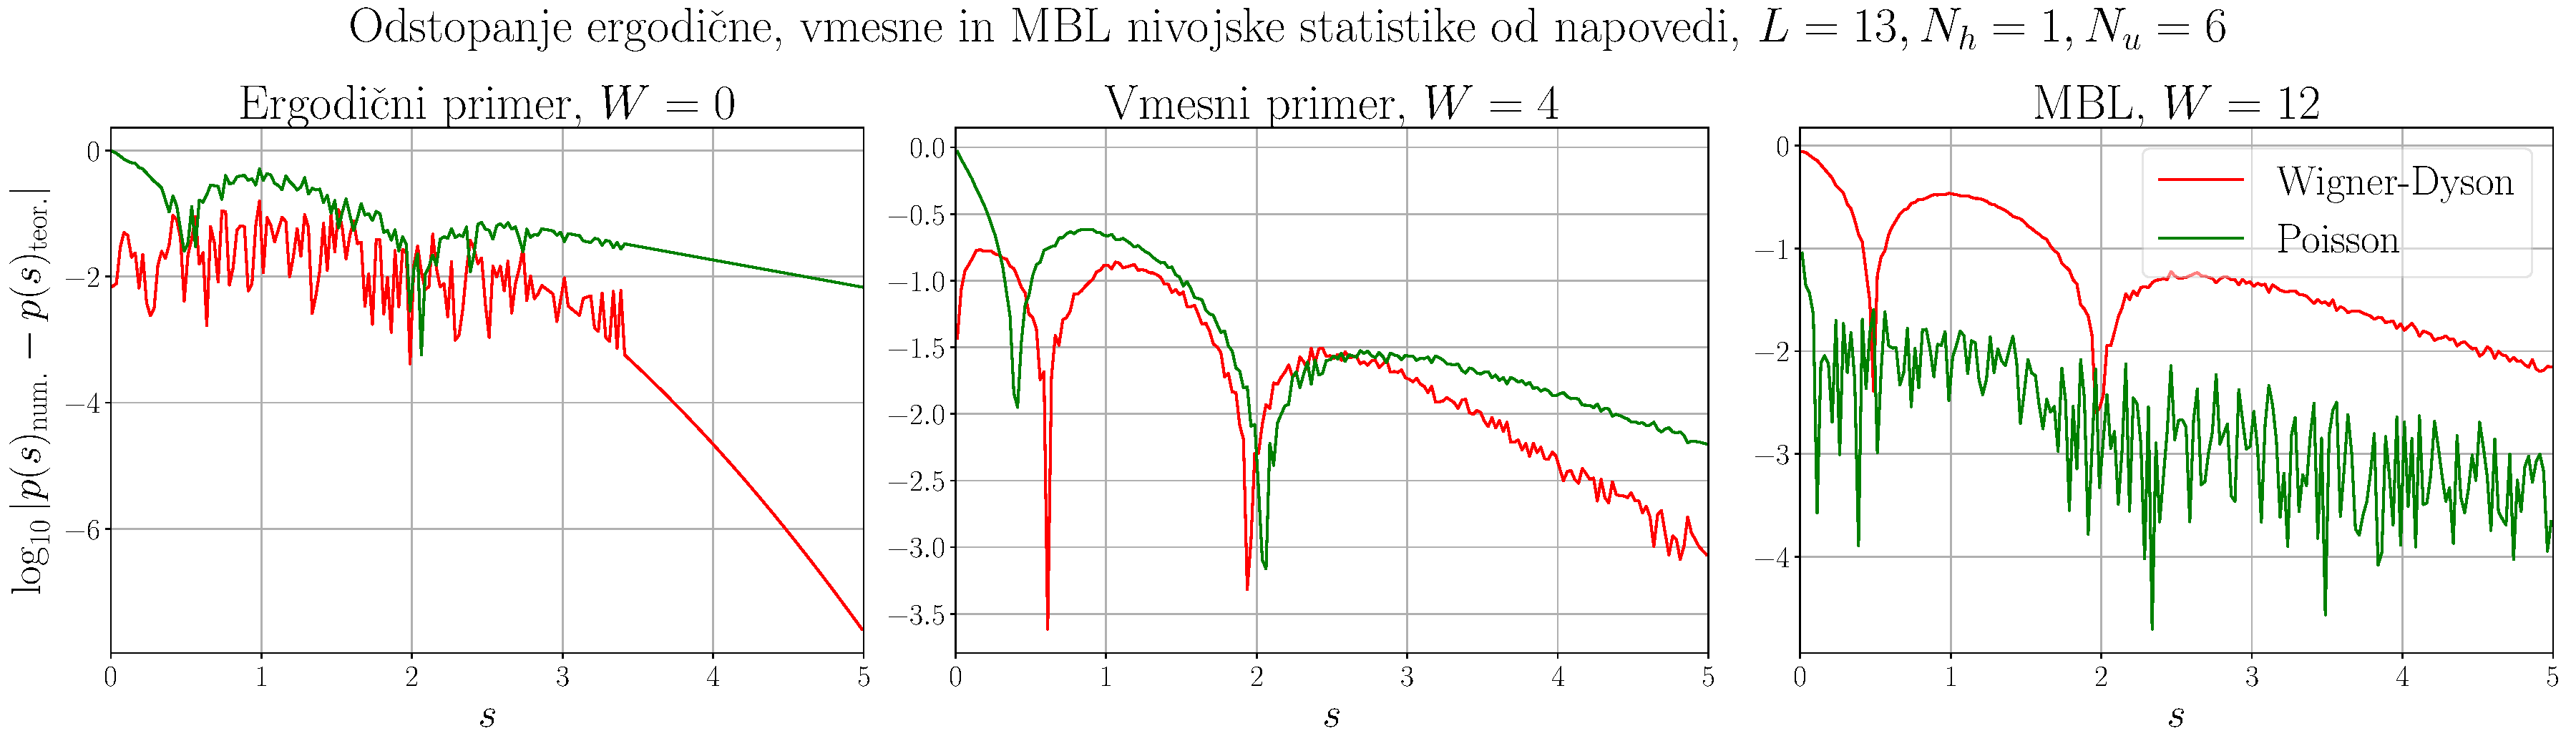
\includegraphics[width=1\textwidth]{unfolding_demo_three_error_slo.pdf}}
\caption{Desetiški logaritem absolutne vrednosti razlike med numerično vrednostjo in teoretično napovedjo za primere izračunov, predstavljene na Sliki~\ref{fig:unfolding_demo_three_slo}. Vsakokrat sta za primerjavo predstavljena izračuna za Wigner-Dysonovo in Poissonovo statistiko. }
\label{fig:unfolding_demo_three_error_slo}
\end{figure}
\noindent
V naslednjih dveh poglavjih sta razložena ključna koraka numerične implementacije izračuna obravnavanih statistik, in sicer razgrnjenje spektra in lokalni zlom simetrije. 
\subsection{Razgrnjenje spektra}
\label{razgrnjenje}
Pred izračunom statistike za razmik med nivoji, podan z En. \eqref{eq:razmik}, moramo izvesti razgrnjenje spektra~\cite{abul2014unfolding}, s katerim povprečni razmik med nivoji fiksiramo na enotsko vrednost. To omogoča medsebojno primerjavo statistike različnih spektrov, ki imajo sicer v splošnem kvantitativno različno gostoto stanj. Slednje je razvidno z grafov na Slikah~\ref{fig:Eigenstates_spin_hole_disorder_13_1_6.pdf} in~\ref{fig:DOS_spin_hole_disorder_13_1_6.pdf}, kjer sprememba parametra nereda znatno vpliva na obliko spektra in gostote stanj. Podobno na gostoto stanj pri enakih vrednostih modelskih parametrov vpliva tudi sprememba velikosti sistema, ki spremeni število stanj. \\\\
Pri diagonalizaciji dobimo spekter po velikosti urejenih lastnih vrednosti $E_i$. \emph{Kumulativno število nivojev} $\tilde{N}(E)$ z energijo, manjšo od $E$, je definirano kot
\begin{equation}\label{eq:unfolding}
\tilde{N}(E)=\sum\limits_{E_i}\Theta(E_i-E),
\end{equation}
gostoto stanj pa določa zveza 
\begin{equation}\label{eq:DOS}
\tilde{\rho}(E)=\frac{\dd \tilde{N}(E)}{\dd E}.
\end{equation}
V odvisnosti $\tilde{N}(E_j),$ kjer je $j$ zaporedni indeks lastnega stanja, je razmik med zaporednimi nivoji po definiciji En. \eqref{eq:unfolding} enak 1. Diskretni kumulativni porazdelitvi $\tilde{N}(E_j)$ priredimo polinomsko krivuljo $g(E_j)$ dovolj visoke stopnje in jo tako zgladimo. V našem programu za prilagoditev krivulje uporabimo funkciji \url{polyfit} in \url{poly1d} iz knjižnice \url{numPy} v programskem jeziku \url{python}.
 Namesto razmika med nivojema $E_n$ in $E_{n+1}$ v energijskem spektru tako spremljamo razmik med nivojema prilagojenega polinoma $g(E_{n})$ in $g(E_{n+1})$. Vlogo razmika med sosednjimi nivoji $s$, podanega z En. \eqref{eq:razmik}, ima tako v naših izračunih v resnici količina $\tilde{s}$, podana kot
$$
\tilde{s}_n=g(E_{n+1})-g(E_n).
$$
V razgrnjenem energijskem spektru je povprečna gostota stanj enaka ena. \\\\
Razgrnitev spektra je potrebna pri izračunih statistike razmikov med sosednjimi nivoji (glej Sliko~\ref{fig:unfolding_demo_three_slo}), pri statistiki razmerij razmikov med sosednjimi nivoji $\tilde{r}$, ki jo podaja En. \eqref{eq:oganesyan_huse}, pa ne. V tem primeru je količina namreč že po definiciji omejena na interval med 0 in 1 in tako nanjo učinki velikosti sistema in spremenljive gostote stanj nimajo vpliva. Primer razgrnitve spektra je prikazan na Sliki~\ref{fig:unfolding_schematics}.
\begin{figure}[H]
\floatbox[{\capbeside\thisfloatsetup{capbesideposition={left,center},capbesidewidth=6.5cm}}]{figure}[\FBwidth]
{\caption{Primer razgrnitve spektra za sistem z $L=5$, $N_h=3$ in $N_u=1$, ki ima 20 stanj. Ker napovedi RMT dobro veljajo za stanja v središču spektra~\cite{d2016quantum}, poleg tega so stanja na robovih spektra občutljivejša na učinke končne velikosti sistema, v izračunih v spektru vselej upoštevamo le polovico stanj med prvim in zadnjim kvartilom vseh stanj, zato je na grafu prikazanih le 10 točk. Kot najprimernejša izbira za glajenje porazdelitve se v tem primeru izkaže kar polinom stopnje 2, pri prevelikih vrednostih $n$ nastopijo težave s slabo pogojenostjo polinomov. Pri večjih sistemih smo tipično uporabljali $n=15.$ }\label{fig:unfolding_schematics}}
{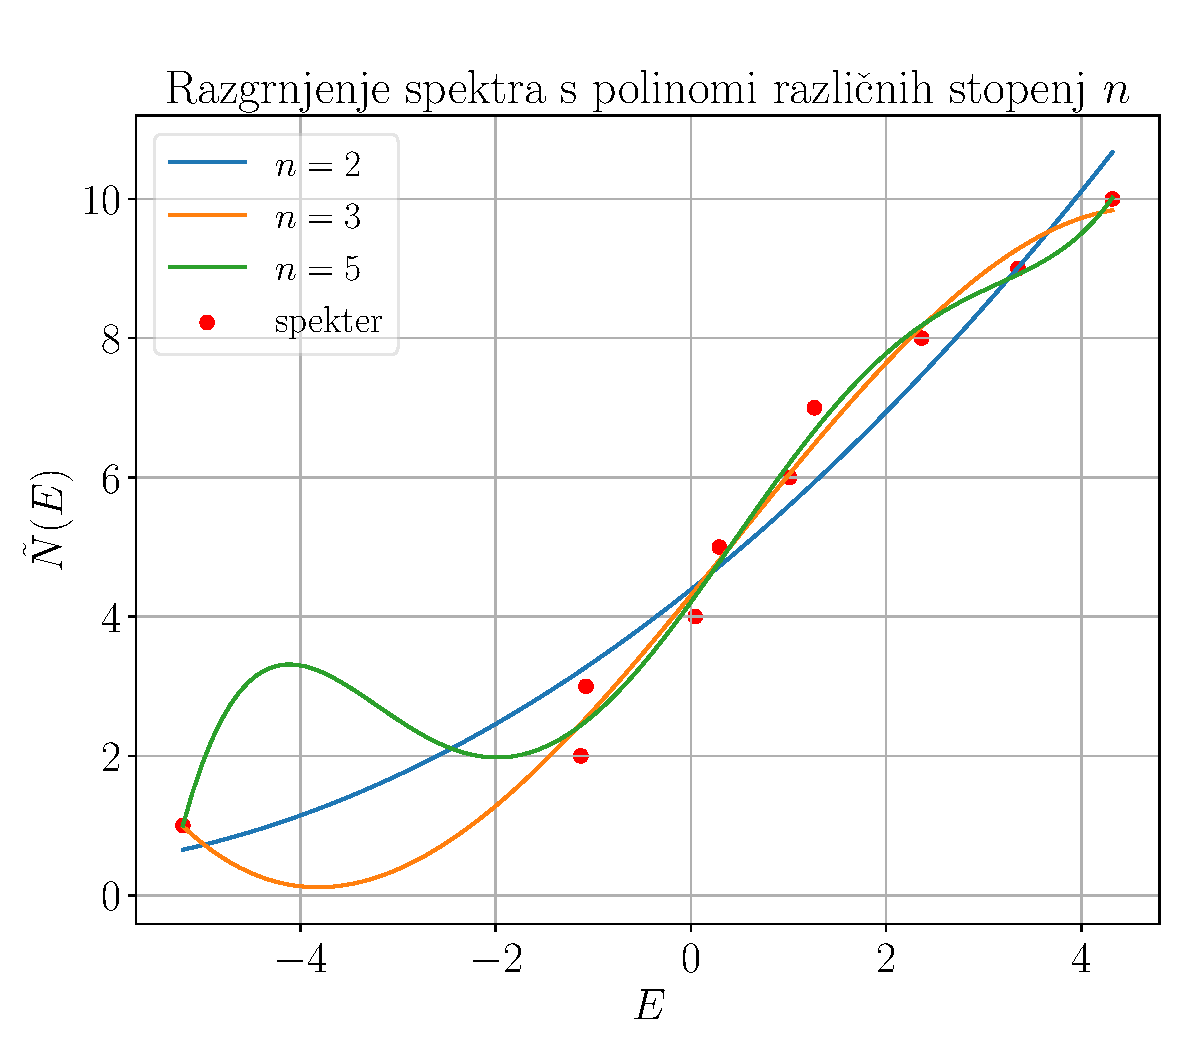
\includegraphics[width=0.55\textwidth]{unfolding_schematics.pdf}}
\end{figure}\newpage
\subsection{Lokalni zlom simetrije}
\label{lokalni_zlom_simetrije}
Obravnava katerekoli izmed do zdaj navedenih nivojskih statistik je smiselna samo v primeru, ko v spektru nimamo degeneracij, ki so posledica nezlomljenih simetrij hamiltonke. Za primerno analizo moramo torej bodisi na primeren način izbrati bazo sistema in spekter preučevati samo na enem izmed simetrijskih podprostorov hamiltonke bodisi moramo hamiltonki dodati šibko perturbacijo, ki zlomi simetrije, vendar bistveno ne spremeni energijske skale sistema. Pri analizi, predstavljeni v magistrski nalogi, uporabljamo drugo možnost, in sicer hamiltonki dodamo lokalna člena, ki se sklapljata s spinom oziroma z vrzeljo:
\begin{equation}\label{eq:sym_break_terms}
h_\mathrm{spin}=W_\mathrm{sym}S_1^z, \hspace{5mm} h_\mathrm{hole}=H_\mathrm{sym}n_L.
\end{equation}
Pri tem sta $W_\mathrm{sym}$ in $H_\mathrm{sym}$ parametra spinskega in vrzelnega zloma simetrije. Njuno najprimernejšo velikost določimo iz pogoja, da moramo v ergodičnem režimu ob odsotnosti vsakršnega nereda za povprečje $\langle\tilde{r} \rangle$ dobiti vrednost $\langle\tilde{r}\rangle_\mathrm{GOE}=0.5307$. Rezultati analize zloma simetrije so prikazani na Sliki~\ref{fig:hole_spin_disorder_sym_break_13_1_6_slo}.

\begin{figure}[H]
\floatbox[{\capbeside\thisfloatsetup{capbesideposition={left,center},capbesidewidth=5cm}}]{figure}[\FBwidth]
{\caption{ Povprečna vrednost $\langle\tilde{r}\rangle$ ob odsotnosti vsakršnega nereda pri skupnem povečevanju parametrov $W_\mathrm{sym}$ in $H_\mathrm{sym}$. V kolikor so v spektru prisotne nezlomljene simetrije, potem statistika ob odsotnosti nereda ni dobro definirana in vrne napačen rezultat. Za vse prikazane velikosti sistema degeneracije učinkovito odpravi vrednost $W_\mathrm{sym}=H_\mathrm{sym}=0.5$, pri čemer vrednost z naraščajočim $L$ pada. Z rdečo in zeleno premico sta označeni vrednosti $\langle \tilde{r}\rangle_\mathrm{GOE}$ oziroma $\langle \tilde{r}\rangle_\mathrm{Poisson}$. }\label{fig:hole_spin_disorder_sym_break_13_1_6_slo}}
{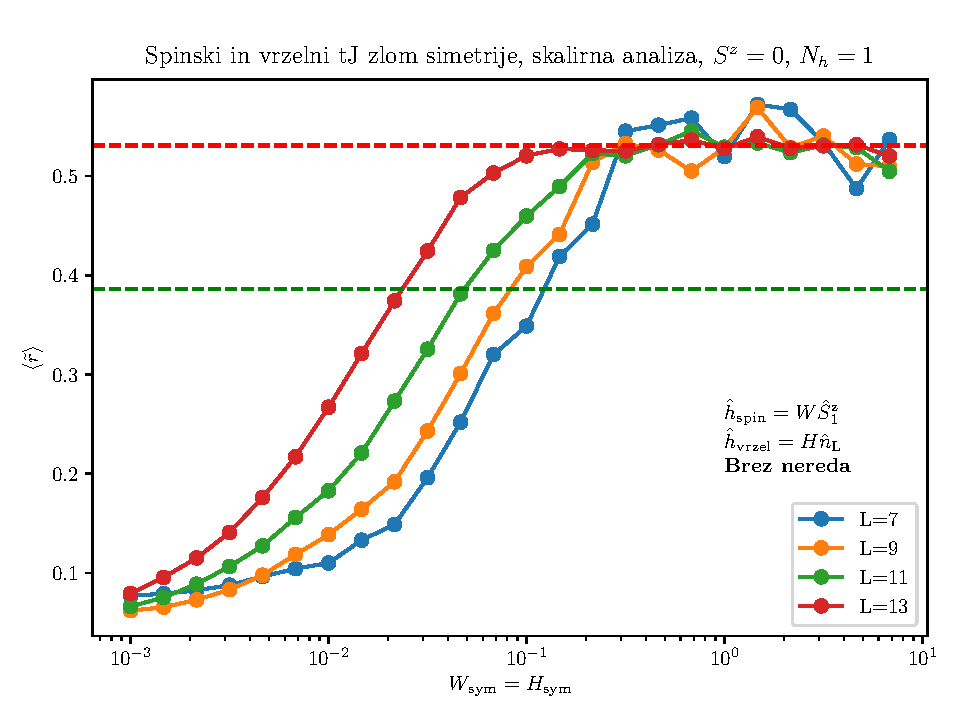
\includegraphics[width=0.7\textwidth]{hole_spin_disorder_sym_break_13_1_6_slo.pdf}}
\end{figure}
\noindent
V kolikor simetrij ne odpravimo, bo porazdelitev nivojske statistike v splošnem konvolucija nivojskih statistik za posamezne simetrijske sektorje hamiltonke. Zaradi morebitnega prekrivanja energijskih nivojev iz različnih simetrijskih sektorjev odboj med nivoji v ergodični fazi v tem primeru ni tako zaznaven. V statistiki razmikov med sosednjimi nivoji to opazimo kot prisotnost neničelne vrednosti $p(s=0)$, povprečje $\langle \tilde{r}\rangle$ pa je manjše, kot bi sicer pričakovali v ergodičnem režimu. Pri vseh nadaljnjih izračunih bomo privzeli $H_\mathrm{sym}=W_\mathrm{sym}=0.5.$ 
%% KO JE TO NAREJENO, NAREDI ŠE SFF in GOSTOTNO PLOSKVICO BOLJ NA FINO (TISTO OD MODELSKE, SAMO MANJŠI INTERVAL, MANJ VREDNOSTI W IN H)
% \newpage
\subsection{Rezultati}
\label{odmik_rezultati}
Z dodanim lokalnim zlomom simetrije so nivojske statistike dobro definirane tudi v primeru odsotnosti vsakršnega nereda - pri $H=W=0$ ima $\langle \tilde{r}\rangle$ vrednost v bližini  $\langle \tilde{r}\rangle_\mathrm{GOE}$. Na Slikah~\ref{fig:double_plot_disorder_sym_break_13_1_6_slo} in~\ref{fig:double_plot_disorder_sym_break_12_4_4_slo} so prikazani rezultati skalirne analize za odvisnost $\langle \tilde{r}\rangle$ v primeru dopiranja z eno vrzeljo in v primeru tretjinskega dopiranja. Na Slikah~\ref{fig:r_density_11_1_5} in~\ref{fig:r_density_9_3_3} sta prikazana še primera sprehodov po prostoru parametrov $H$ in $W$ pri izračunu $\langle \tilde{r} \rangle$.
 \begin{figure}[H]
\centering{
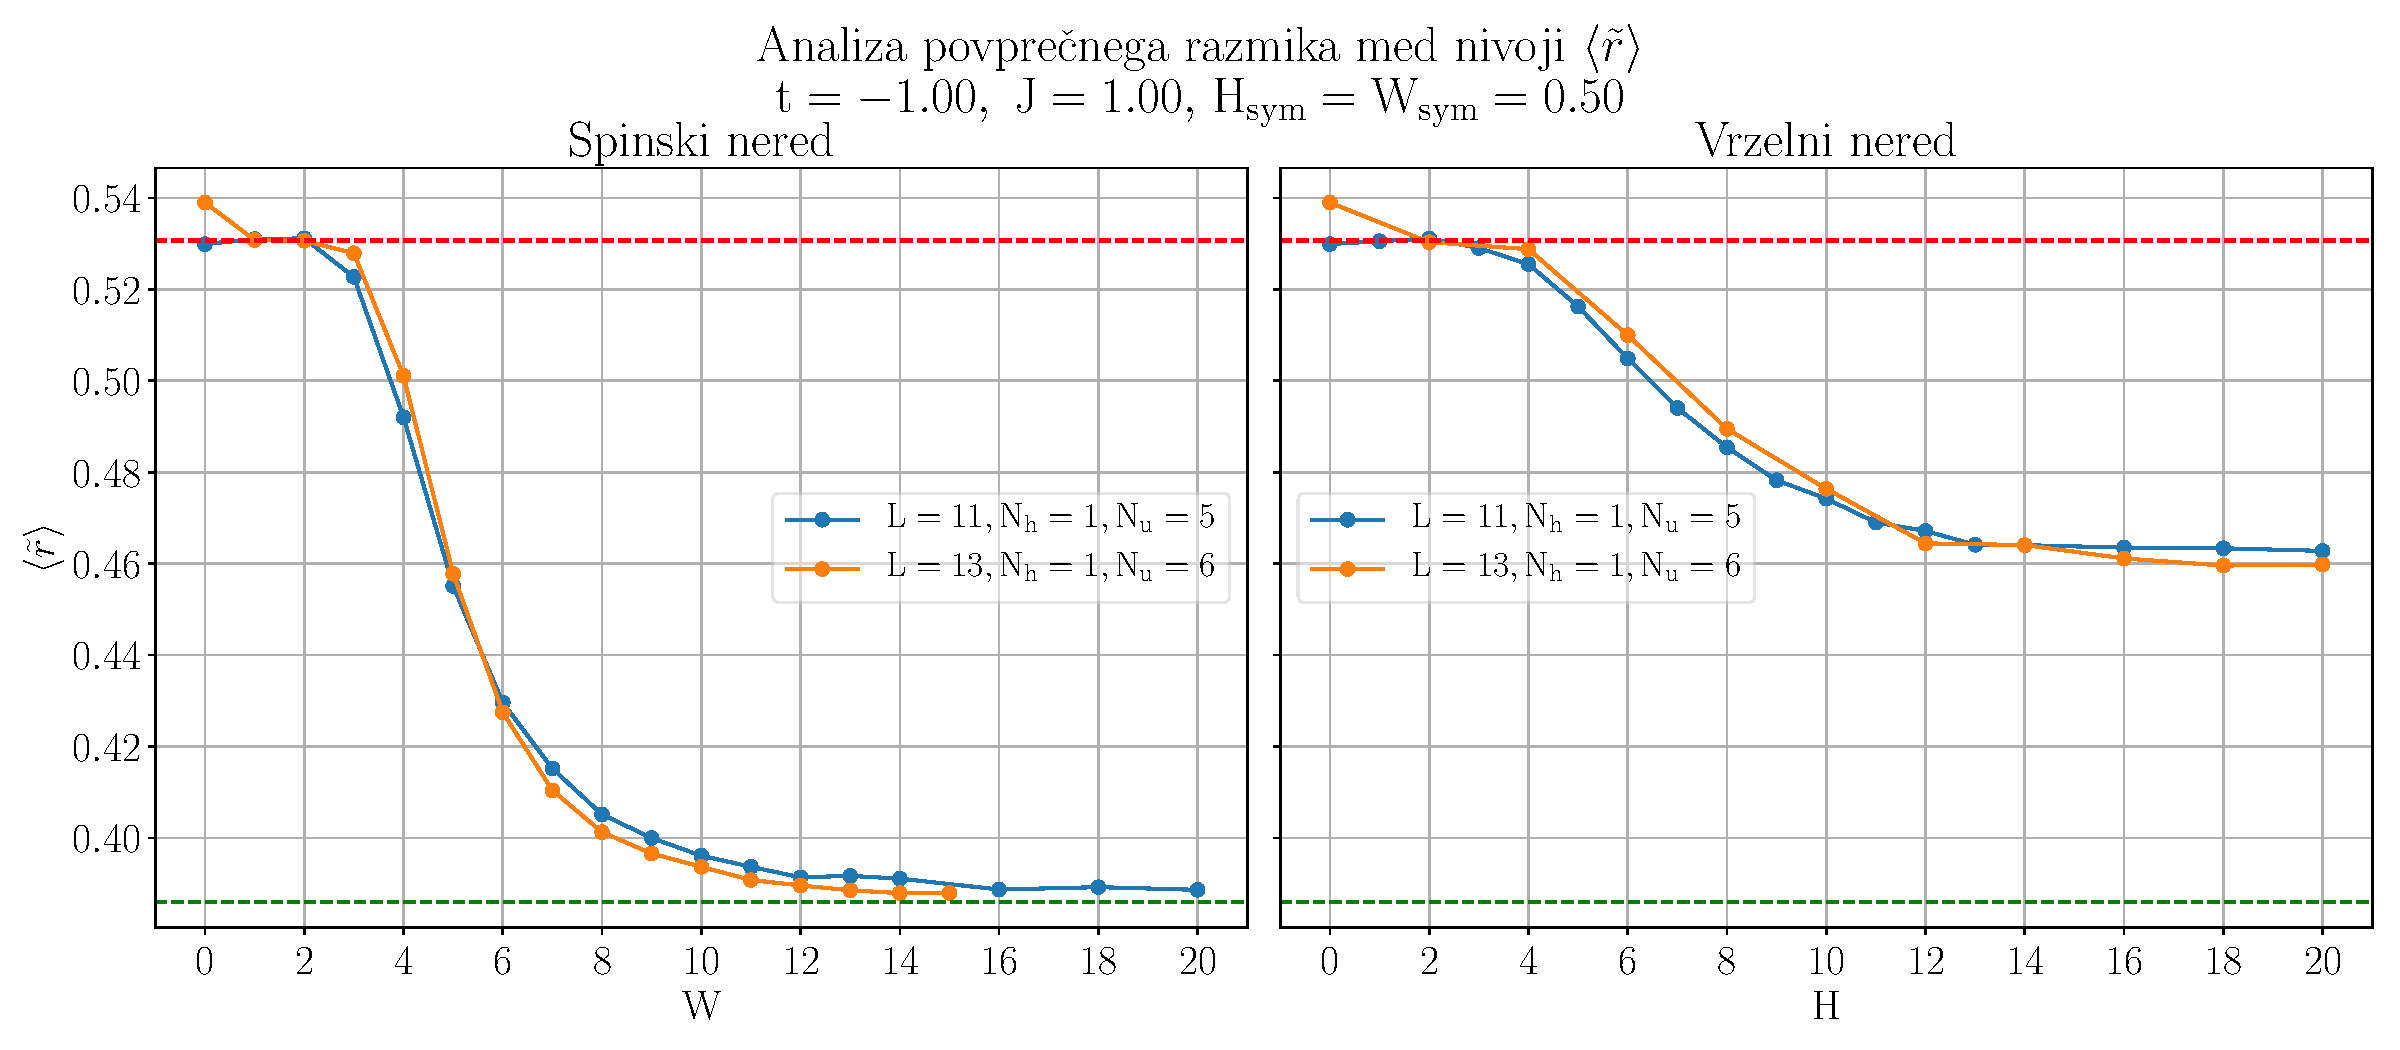
\includegraphics[width=1\textwidth]{double_plot_disorder_sym_break_13_1_6_slo.pdf}}
\caption{Zaradi majhnega števila primernih sistemov (sistemi z $L<9$ imajo premalo stanj za primerno statistiko, sistemi z $L>15$ so preveliki za naše računske zmogljivosti) je skalirna analiza, ki bi omogočila ekstrapolacijo rezultatov proti termodinamski limiti neskončnega sistema, razmeroma zahtevna če ne nemogoča naloga. Kljub temu lahko sklepamo, da v primeru ene vrzeli povečevanje spinskega nereda vodi do prehoda v MBL režim, medtem ko nered, ki se sklaplja z vrzelmi, ne pripelje do večdelčne lokalizacije. Nekoliko presenetljivo se zdi, da se v primeru vrzelnega nereda vrednost $\langle \tilde{r}\rangle$ z naraščanjem $L$ pomika navzdol, saj bi v termodinamski limiti pričakovali, da bo prispevek nereda na eni vrzeli zanemarljivo majhen. }
\label{fig:double_plot_disorder_sym_break_13_1_6_slo}
\end{figure} 
\begin{figure}[H]
\centering{
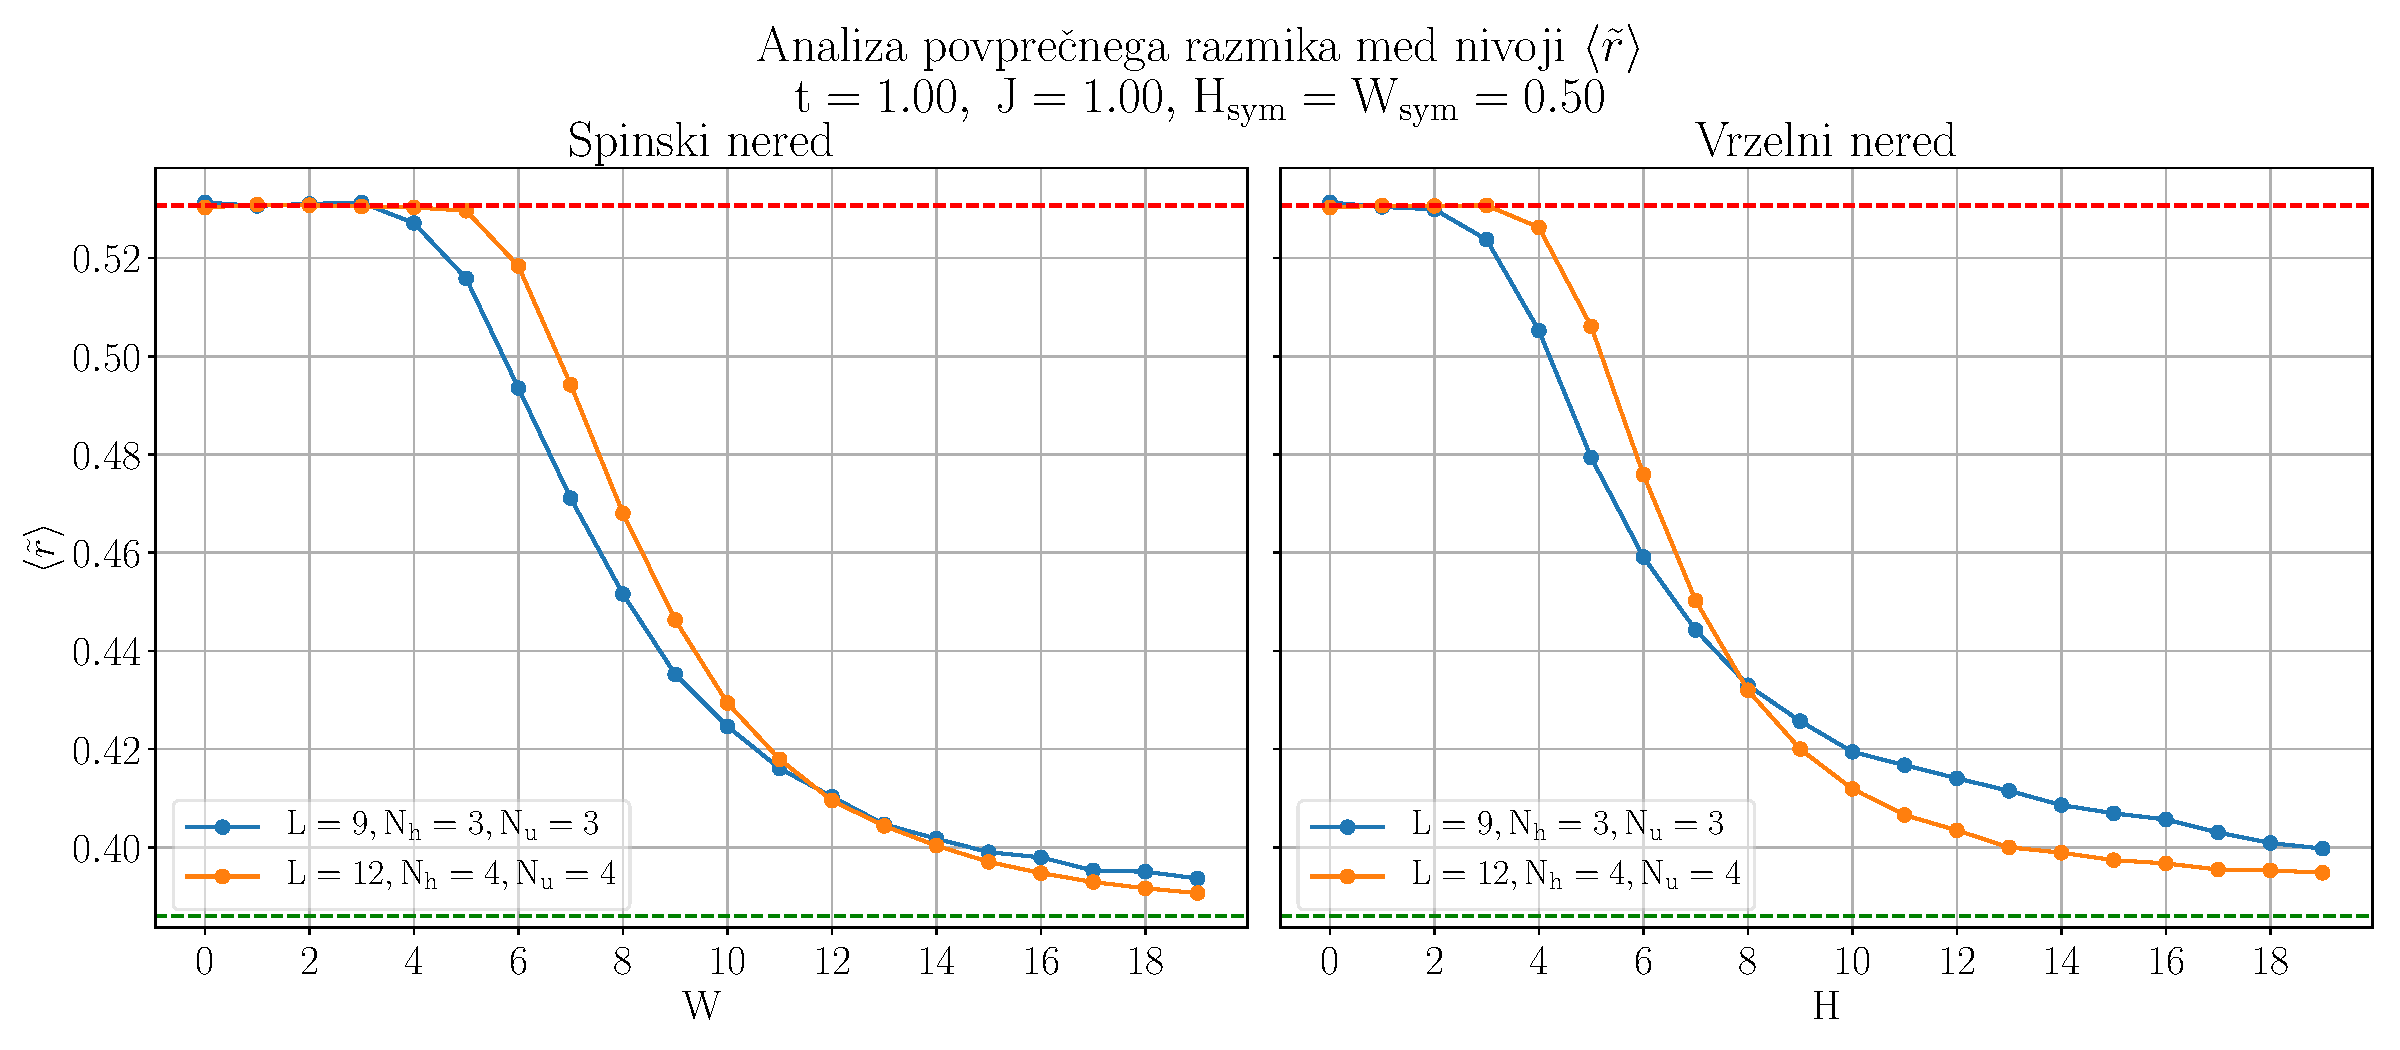
\includegraphics[width=1\textwidth]{double_plot_disorder_sym_break_12_4_4_slo.pdf}}
\caption{Pri tretjinskem dopiranju se zdi, da lahko oba tipa nereda pripeljeta do večdelčne lokalizacije. Krivulja za $L=6$ je statistično nepomembna, saj ima ta sistem zgolj 90 stanj, kar je očitno premalo za zanesljivo statistiko. Fluktuacije povprečnih količin namreč padajo z velikostjo sistema. Zaradi omejenega števila sistemov, ki so na voljo za preučevanje, je skalirna analiza, s katero bi določil, kje v termodinamski limiti neskončnega sistema pride do prehoda med MBL in ergodičnim sistemom, otežena.  }
\label{fig:double_plot_disorder_sym_break_12_4_4_slo}
\end{figure}
\begin{figure}[H]
\floatbox[{\capbeside\thisfloatsetup{capbesideposition={left,center},capbesidewidth=5cm}}]{figure}[\FBwidth]
{\caption{Vrednosti $\langle \tilde{r}\rangle$ v odvisnosti od $H$ in $W$ za primer dopiranja z eno vrzeljo pri velikosti sistema $L=11$ ter povprečenjem po 500 naključnih realizacijah za obe vrsti nereda. Modra oz. temnejši toni označuje(jo) MBL režim, rumeni in zeleni odtenki pa pomenijo ergodičnost. Pri majhnem spinskem neredu opazimo, da še tako velike vrednosti $H$ ne pripeljejo do lokalizacije. }\label{fig:r_density_11_1_5}}
{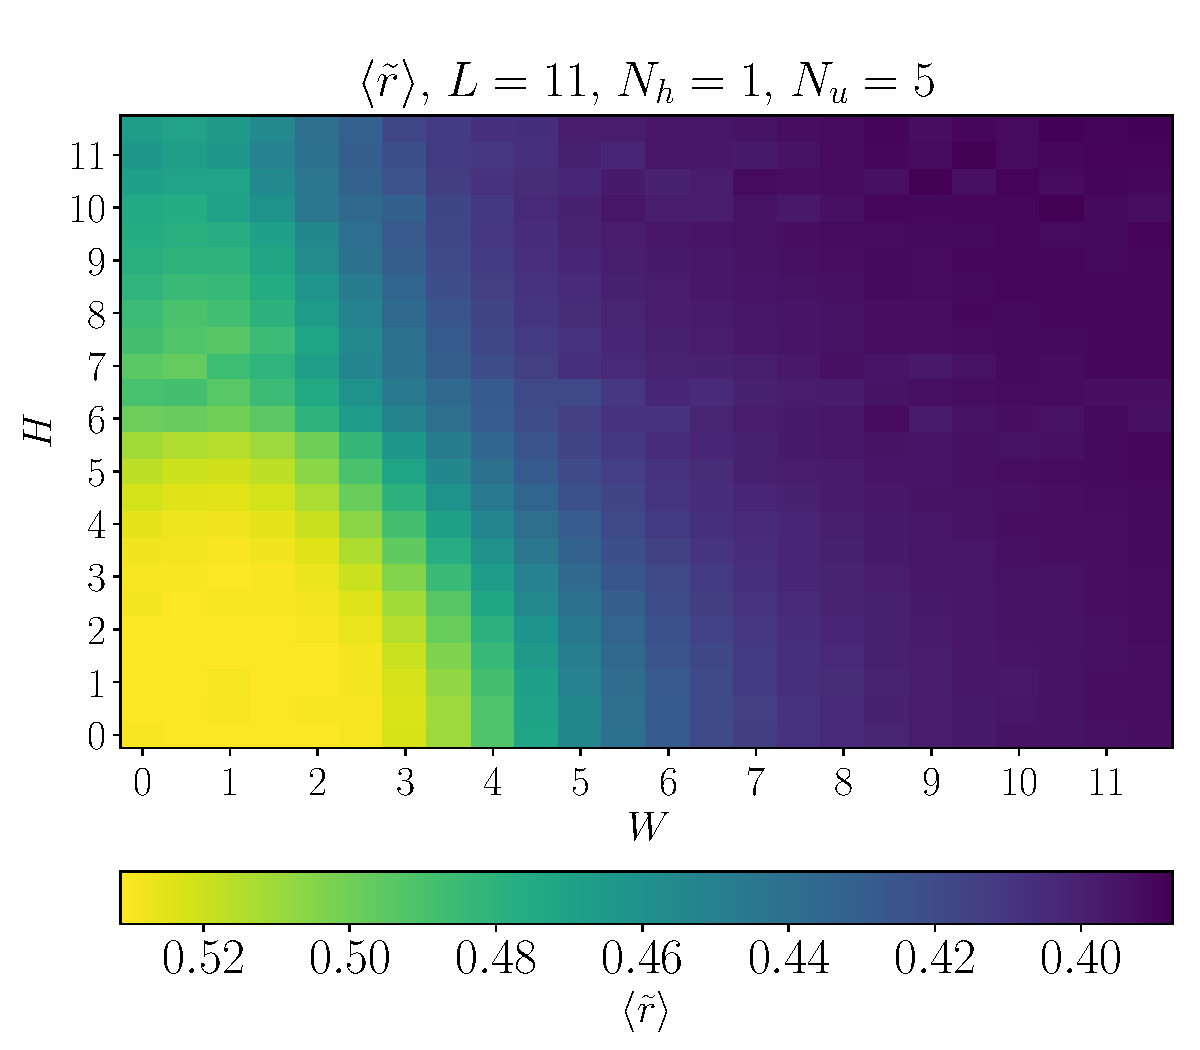
\includegraphics[width=0.6\textwidth]{r_density_11_1_5.pdf}}
\end{figure}
\begin{figure}[H]
\floatbox[{\capbeside\thisfloatsetup{capbesideposition={left,center},capbesidewidth=5cm}}]{figure}[\FBwidth]
{\caption{Sprehod po prostoru parametrov $H$ in $W$ pri izračunu $\langle \tilde{r}\rangle$ še za primer tretjinskega dopiranja in ponovno povprečenja po 500 naključnih realizacijah nereda, $L=9$. Spreminjanje obeh parametrov vodi do lokalizacije, pri čemer se zdi vloga obeh parametrov dokaj enakovredna. }\label{fig:r_density_9_3_3}}
{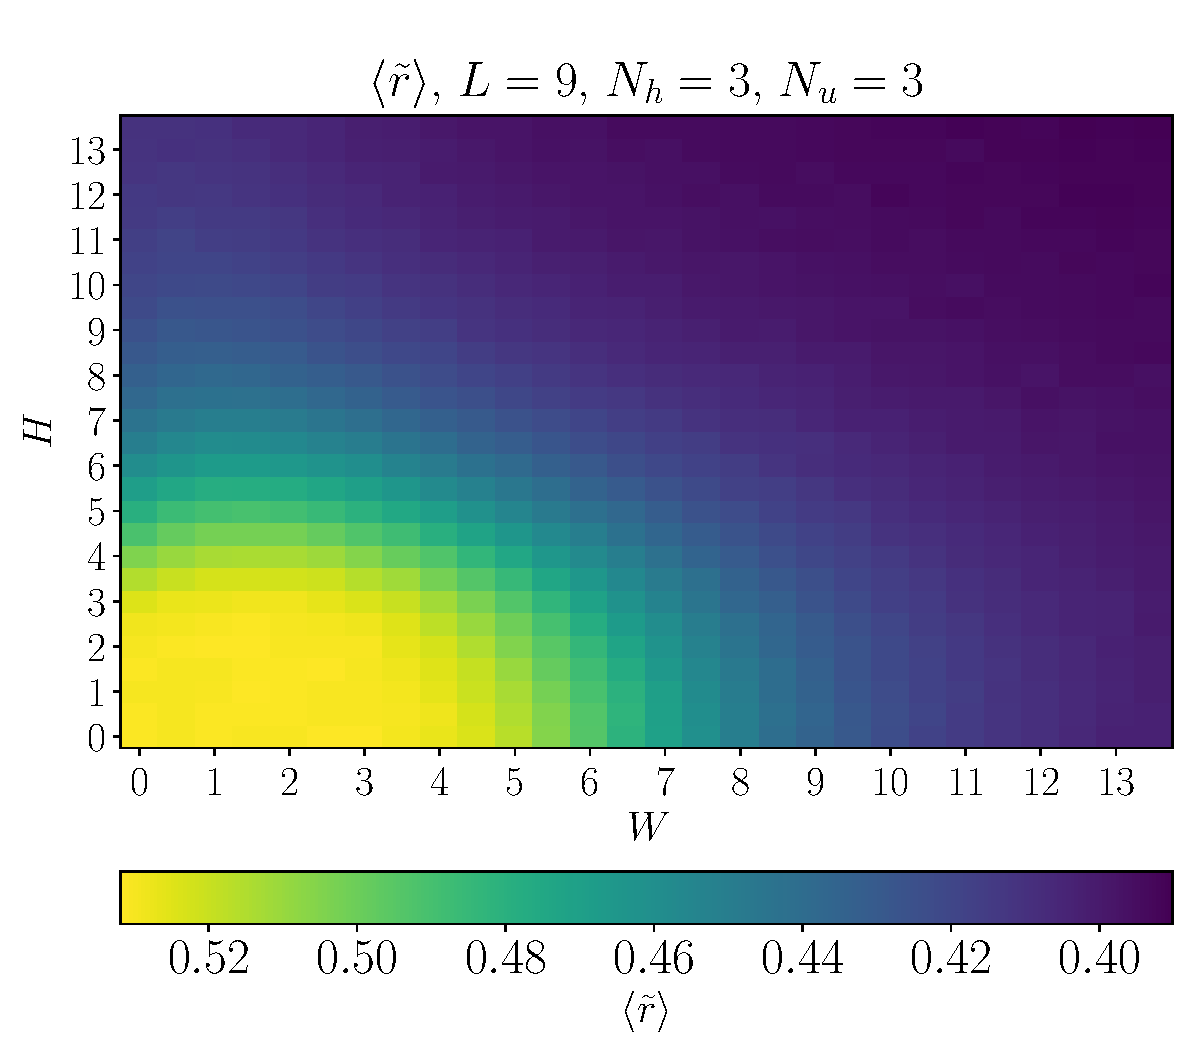
\includegraphics[width=0.6\textwidth]{r_density_9_3_3.pdf}}
\end{figure}
\noindent
Za primer dopiranja z eno vrzeljo in v prisotnosti spinskega nereda, ki ga modelira parameter $W$, so zgornji rezultati skladni z nedavno napovedjo prehoda med ergodično in MBL fazo pri povečevanju parametra velikosti spinskega nereda (Lemut in dr.,~\cite{lemut2017complete}). V primeru prisotnosti vrzelnega nereda komplementarne študije časovne dinamike začetnih stanj (Bonča in Mierzejewski,~\cite{PhysRevB.95.214201}) pri dopiranju z eno vrzeljo kažejo na odsotnost MBL faze. Naši rezultati napovedi niti ne potrdijo niti ne ovržejo, saj kažejo na vmesno obnašanje, ki ni značilno za nobeno izmed obravnavanih faz. Za natančnejši opis bi bila potrebna analiza precej večjih sistemov, ki pa so s polno diagonalizacijo nedosegljivi. 
\newpage
 \section{Spektralni oblikovni faktor}
V tem poglavju namesto korelacij med zgolj sosednjimi energijskimi nivoji obravnavamo korelacije med \emph{vsemi} energijskimi nivoji, in sicer z analizo \emph{spektralnega oblikovnega faktorja} (ang.~\emph{spectral form factor}). Količino najprej vpeljemo, nato pa predstavimo rezultate numeričnih analiz, s katerimi smo presojali ergodičnost oziroma prisotnost večdelčne lokalizacije v obravnavanih sistemih. 
\label{spektralni_oblikovni_faktor}
\subsection{Vpeljava}
Obravnava korelacij med vsemi energijskimi nivoji omogoča podrobnejši vpogled v spektralne lastnosti sistema in posledično podaja popolnejšo sliko prehoda med ergodično in lokalizirano fazo. V poglavju~\ref{statistika_sosednjih_nivojev} predstavljeni spektralni statistiki, v okviru katerih smo prehod preučevali do zdaj, namreč upoštevata le razmike med sosednjimi energijskimi nivoji, kar ustreza najmanjši energijski skali sistema, in zato opisujeta obnašanje sistema v dolgočasovni limiti. Kot smo zapisali v poglavju~\ref{lokalizacija_v_sistemih_z_med}, dolgočasovni razvoj pri relaksaciji začetnega stanja najkasneje izniči izvendiagonalne matrične elemente med stanji, katerih energije se le malo razlikujejo (glej En.~\eqref{eq:ergodicnost_kvantno}). Z upoštevanjem korelacij med vsemi energijskimi nivoji dobimo tudi vpogled v obnašanje sistema na vseh časovnih skalah. \\\\
\emph{Dvotočkovna korelacijska funkcija} diskretnega energijskega spektra je definirana kot 
\begin{equation}\label{eq:engy_correlation}
R(E)=\frac{1}{N}\sum\limits_{i,j=1}^N\delta\left(E_i - E_j - E\right),
\end{equation}
kjer sta $E_i$ in $E_j$ energiji v spektru, $N$ pa število stanj v njem. Spektralni oblikovni faktor $K(\tau)$ vpeljemo kot Fourierovo transformacijo $R(E)$~\cite{chen2017universal}
\begin{equation}\label{eq:SFF}
K(\tau)\coloneqq \left\langle\int\limits_{-\infty}^\infty  \mathrm{e}^{-\iu E \tau}R(E)\dd E \right\rangle = \left\langle \frac{1}{N}\sum\limits_{i,j}^N \mathrm{e}^{-\iu \left(E_i - E_j\right) \tau}\right\rangle.
\end{equation}
Pri tem je $\left\langle\dots\right\rangle$ povprečenje, ki smo ga pri naših izračunih vselej izvedli po spektrih, izračunanih za različne realizacije nereda. S $\tau$ smo označili realni parameter časa. Pri računanju upoštevamo, da velja
\begin{equation}
K(\tau)=\left\langle Z(\tau)Z(\tau)^* \right\rangle,
\end{equation}
kjer smo zapisali
\begin{equation}
Z(\tau)=\frac{1}{\sqrt{N}}\sum\limits_i \mathrm{e}^{-\iu E_i \tau}.
\end{equation}
Iz En.~\eqref{eq:SFF} sta nemudoma očitni vrednosti $K(\tau)$ v limitah $\tau\to0$ in $\tau\to\infty$. V prvem primeru so vsi členi v dvojni vsoti enaki ena in je zato $K(\tau=0)=N.$ V skladu s povedanim v poglavju~\ref{lokalizacija_v_sistemih_z_med} dolgočasovni razvoj izniči izvendiagonalne člene v vsoti, zato po dolgem času k vsoti prispeva le $N$ diagonalnih členov in je $K(\tau\to\infty)=1.$\\\\
Kot pri spektralnih statistikah, obravnavanih v poglavju~\ref{statistika_sosednjih_nivojev}, je tudi tokrat za našo analizo najpomembnejše dejstvo, da ima SFF v različnih tipih sistemov univerzalne lastnosti, kar izkoristimo pri razločevanju med ergodično in MBL fazo. Začenši pri $\tau=0$ funkcija $K(\tau)$ za kratke čase uvodoma pada, vse dokler ne doseže minimalne vrednosti. Relaksacija $K(\tau)$ proti minimalni vrednosti ni univerzalna temveč modelsko specifična, saj jo v En.~\eqref{eq:SFF} določajo členi z velikimi energijskimi razlikami $E_i-E_j.$ Čas, po katerem $K(\tau)$ ne kaže več neuniverzalnih lastnosti in preide v univerzalni režim, se v literaturi pogosto označuje kot \emph{Thoulessov čas} $\tau_\mathrm{T}.$ Univerzalna lastnost $K(\tau)$ je  za ergodične sisteme območje linearne rasti (ang.~\emph{ramp}), ki nastopi med $\tau_\mathrm{T}$ in \emph{Heisenbergovim časom} $\tau_\mathrm{H},$ po katerem $K(\tau)$ saturira pri limitni vrednosti. Heisenbergov čas je definiran kot
\begin{equation}
\tau_\mathrm{H}=2\pi\bar{\tilde{\rho}},
\end{equation}
kjer je $\bar{\tilde{\rho}}$ povprečna gostota stanj. Ker tudi izračune $K(\tau)$ izvajamo na razgrnjenem spektru, ima $\bar{\tilde{\rho}}$ v naših računih enotsko vrednost, $\bar{\tilde{\rho}}=1.$ V nadaljevanju bomo čas $\tau$ vselej podajali v enotah $\tau_\mathrm{H},$ kot je to v navadi v literaturi. V teh enotah saturacija nastopi pri $\tau=\tau_\mathrm{H}=1.$\\\\
V sistemih, katerih spektralne lastnosti ustrezajo GOE sistemom, podaja univerzalno obnašanje $K(\tau)$ zveza~\cite{sieber2001correlations}
\begin{equation}\label{eq:ramp}
K_\mathrm{GOE}(\tau)=
\begin{cases}
2\tau - \tau \log\left(1 + 2\tau\right), \hspace{5mm} \tau \leq 1, \\
2 - \tau \log\left(\frac{2\tau + 1}{2\tau - 1}\right),\hspace{5mm} \tau >1.
\end{cases}
\end{equation} 
V naši numerični analizi smo se osredotočili predvsem na prvi primer, ki za čase, manjše od $\tau_\mathrm{H},$ napoveduje linearno rast $K(\tau)$ z logaritemskim popravkom. V sistemih s Poissonovo spektralno statistiko je v univerzalnem režimu $K(\tau)$ enak konstanti, in sicer je~\cite{kos2018many}
\begin{equation}
K_\mathrm{Poisson}(\tau)=\tau_\mathrm{H}=1.
\end{equation}
Očitno razliko med $K_\mathrm{GOE}(\tau)$ in $K_\mathrm{Poisson}(\tau)$ izkoristimo pri presoji ergodičnosti oziroma lokaliziranosti preučevanih sistemov, saj v ergodičnih sistemih za $\tau\leq1$ na nekem končnem časovnem intervalu pričakujemo linearno rast, v lokaliziranih sistemih pa ne. Primera $K(\tau)$ v ergodičnem in MBL primeru sta prikazana na levem grafu na Sliki~\ref{fig:scheme_sff_disorder_14_0_7}. Prikazani so rezultati za izotropno Heisenbergovo verigo, enega najpogosteje preučevanih modelov MBL.\\\\
V praksi za preučevanje spektralnih lastnosti namesto $K(\tau)$ uporabljamo \emph{povezani spektralni oblikovni faktor} $K_c(\tau),$ ki je definiran kot~\cite{chen2017universal} 
\begin{equation}\label{eq:SFF_connected}
K_c(\tau)=K(\tau) - \left\langle Z(\tau) \right\rangle \left\langle Z(\tau)^*\right\rangle=\left\langle \abs{Z(\tau)}^2 \right\rangle - \abs{\left\langle Z(\tau)\right\rangle}^2.
\end{equation}
Tudi za $K_c(\tau)$ veljajo zgoraj zapisane univerzalne napovedi, vendar je časovni interval zaznanega univerzalnega obnašanja tipično daljši kot pri izračunu $K(\tau).$ S členom $\abs{\left\langle Z(\tau)\right\rangle}^2$ smo namreč odšteli prispevek neuniverzalnih fluktuacij, ki so v En.~\eqref{eq:SFF} posledica prispevkov členov z velikimi razlikami energij $E_i-E_j.$ Za kratke čase lahko omenjene fluktuacije prikrijejo univerzalne lastnosti spektra. Na desnem grafu na Sliki~\ref{fig:scheme_sff_disorder_14_0_7} sta prikazana izračuna $K_c(\tau)$ v ergodičnem in MBL primeru. 
 \begin{figure}[H]
\centering{
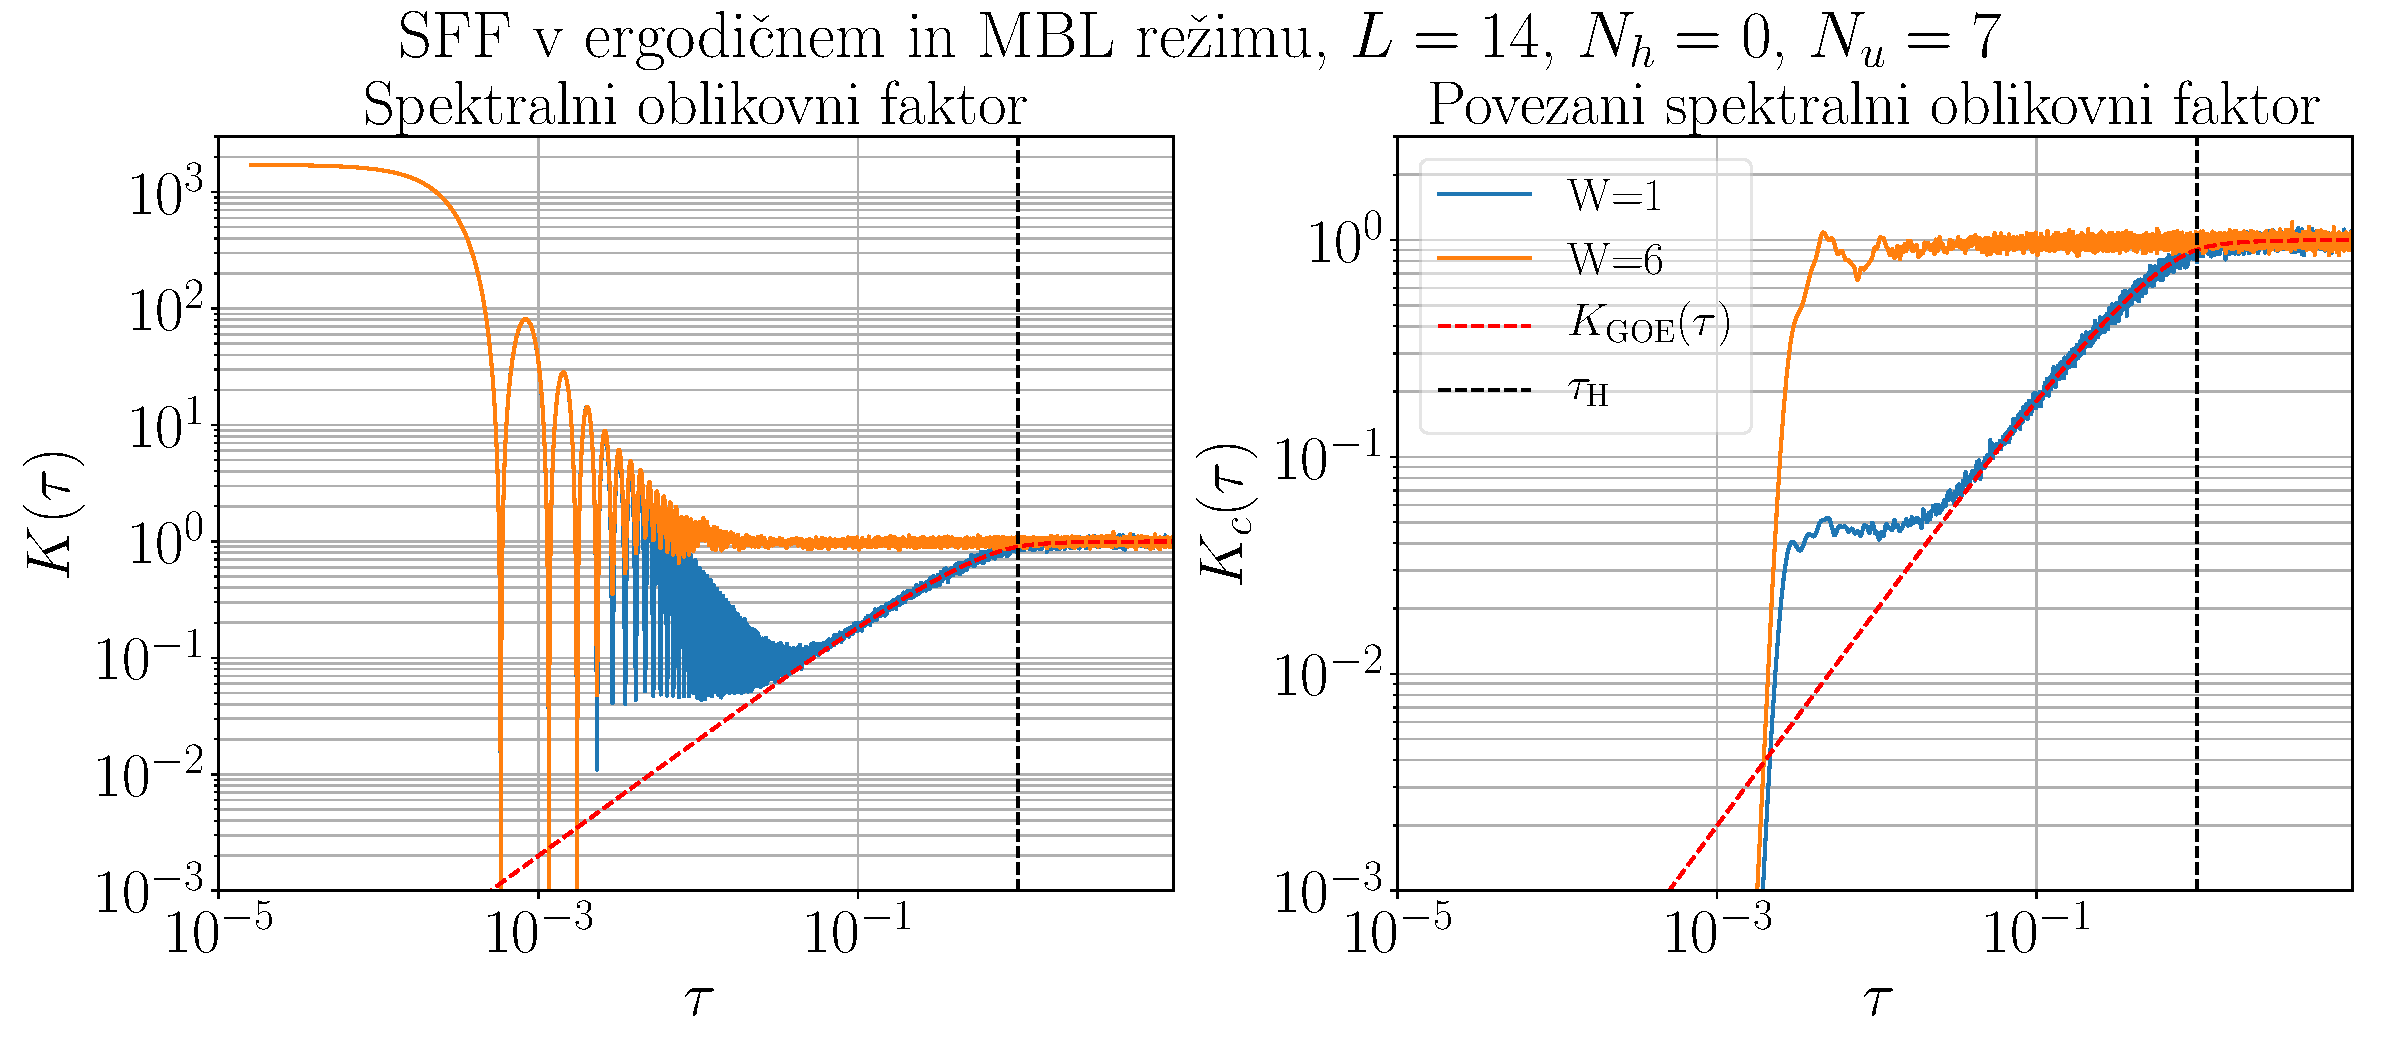
\includegraphics[width=1\textwidth]{scheme_sff_disorder_14_0_7.pdf}}
\caption{Izračun $K(\tau)$ in $K_c(\tau)$ v ergodičnem ($W=1$) in MBL ($W=6$) primeru za model $t$-$J$ brez vrzeli in naključnim magnetnim poljem, ki ustreza izotropnemu Heisenbergovemu modelu z $J=1$, ki ga podaja En.~\eqref{eq:XXZ}. Prehod med ergodično in lokalizirano fazo nastopi pri kritični vrednosti parametra nereda $W^*\approx 3.5$~\cite{pal2010many}. Levo: za kratke čase zavzame $K(\tau)$ največjo vrednost, nato v neuniverzalnem režimu pada. V ergodičnem primeru neuniverzalnemu obnašanju sledi linearna rast v skladu z En.~\eqref{eq:ramp}, ki jo označuje rdeča črtkana črta. V MBL primeru linearne rasti ne opazimo, po neuniverzalni relaksaciji ostane $K(\tau)$ enak konstanti. 
Desno: izračun $K_c(\tau),$ kjer smo od $K(\tau)$ odšteli neuniverzalne prispevke členov z velikimi razlikami energij. 
Pred izračunom obeh količin smo energijska spektra razgrnili in kot v predhodnem poglavju upoštevali le polovico vrednosti med prvim in zadnjim kvartilom. Čas $\tau$ je podan v enotah $\tau_\mathrm{H},$ povprečenje pa smo izvedli po 500 različnih realizacijah nereda. }
\label{fig:scheme_sff_disorder_14_0_7}
\end{figure}  
% \subsection{Rezultati}
\newpage
\subsection{Rezultati}
Spektralni oblikovni faktor smo za model $t$-$J$ izračunali v primeru dopiranja z eno vrzeljo in v primeru tretjinskega dopiranja. Kot v poglavju~\ref{statistika_sosednjih_nivojev} smo pred izračunom $K(\tau)$ in $K_c(\tau)$ izvedli razgrnjenje spektra ter količini izračunali za polovico lastnih energij med prvim in zadnjim kvartilom v spektru. Povprečenje smo, odvisno od velikosti dimenzije Hilbertovega prostora sistema, izvedli po 100 do 600 realizacijah nereda. \\\\
Na Slikah~\ref{fig:W_sweep_sff_disorder_11_1_5} in~\ref{fig:H_sweep_sff_disorder_11_1_5}
so prikazani rezultati izračuna $K(\tau)$ in $K_c(\tau)$ pri dopiranju z eno vrzeljo za različne vrednosti parametrov velikosti spinskega oziroma potencialnega nereda, kjer smo povprečenje izvedli po 500 realizacijah nereda. 
% \begin{equation}
% \Delta K_c(\tau) = \abs{\frac{K_c(\tau) - K_\mathrm{GOE}(\tau)}{K_\mathrm{GOE}(\tau)}}
% \end{equation}
 \begin{figure}[H]
\centering{
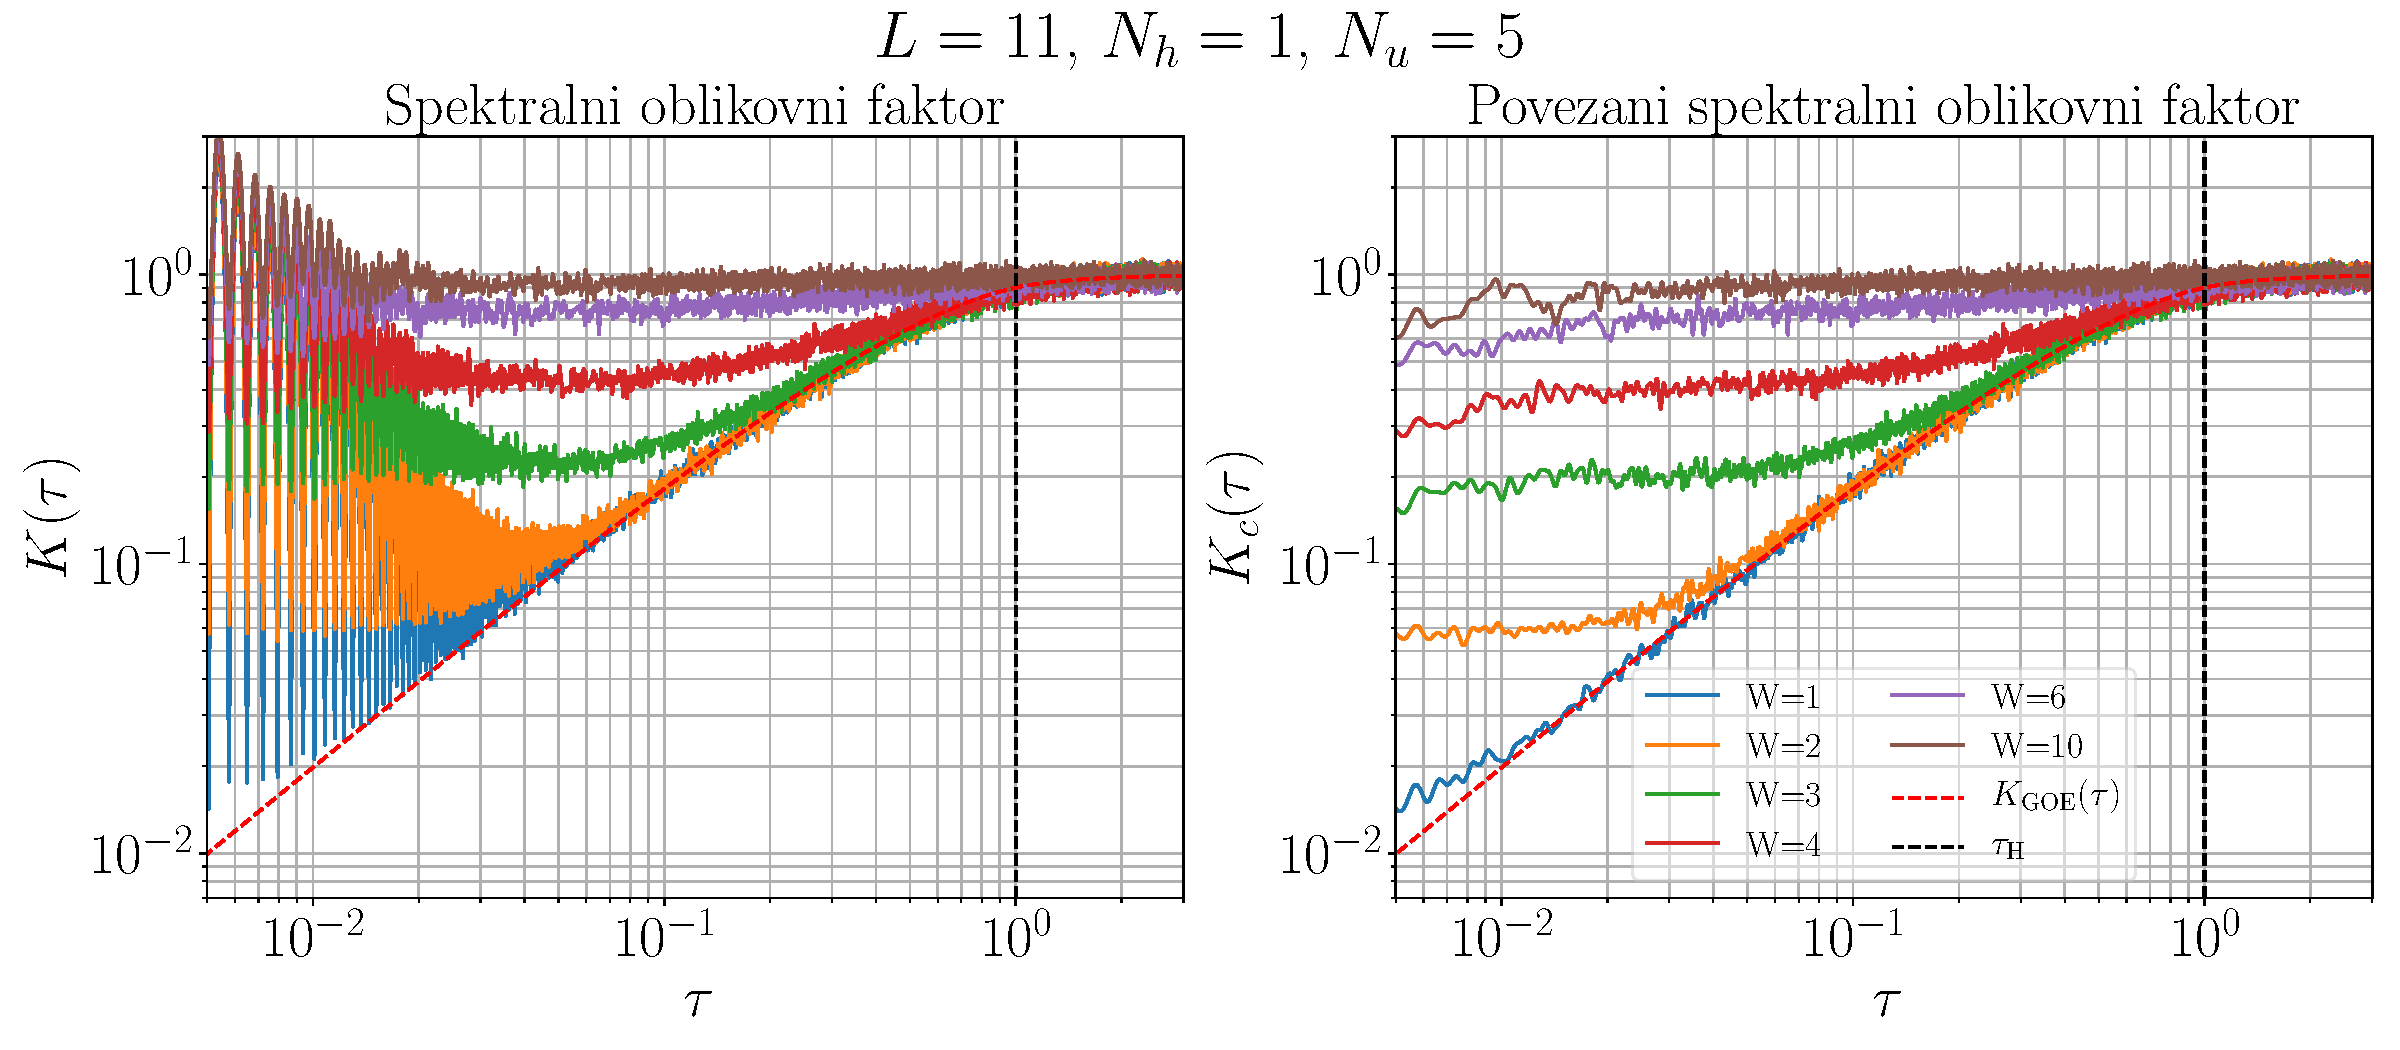
\includegraphics[width=0.93\textwidth]{W_sweep_sff_disorder_11_1_5.pdf}}
\caption{$K(\tau)$ in $K_c(\tau)$ pri različnih vrednostih parametra velikosti spinskega nereda $W$. S povečevanjem $W$ se univerzalni linearni del krivulje, ki sovpada s krivuljo $K_\mathrm{GOE}(\tau)$, manjša, odvisnost pa se v univerzalnem območju vse bolj približuje napovedi $K_\mathrm{Poisson}(\tau).$ Ujemanje rezultatov s teoretičnimi napovedmi je podrobneje predstavljeno na Sliki~\ref{fig:double_sweep_sff_disorder_11_1_5_four}}
\label{fig:W_sweep_sff_disorder_11_1_5}
\end{figure}
 \begin{figure}[H]
\centering{
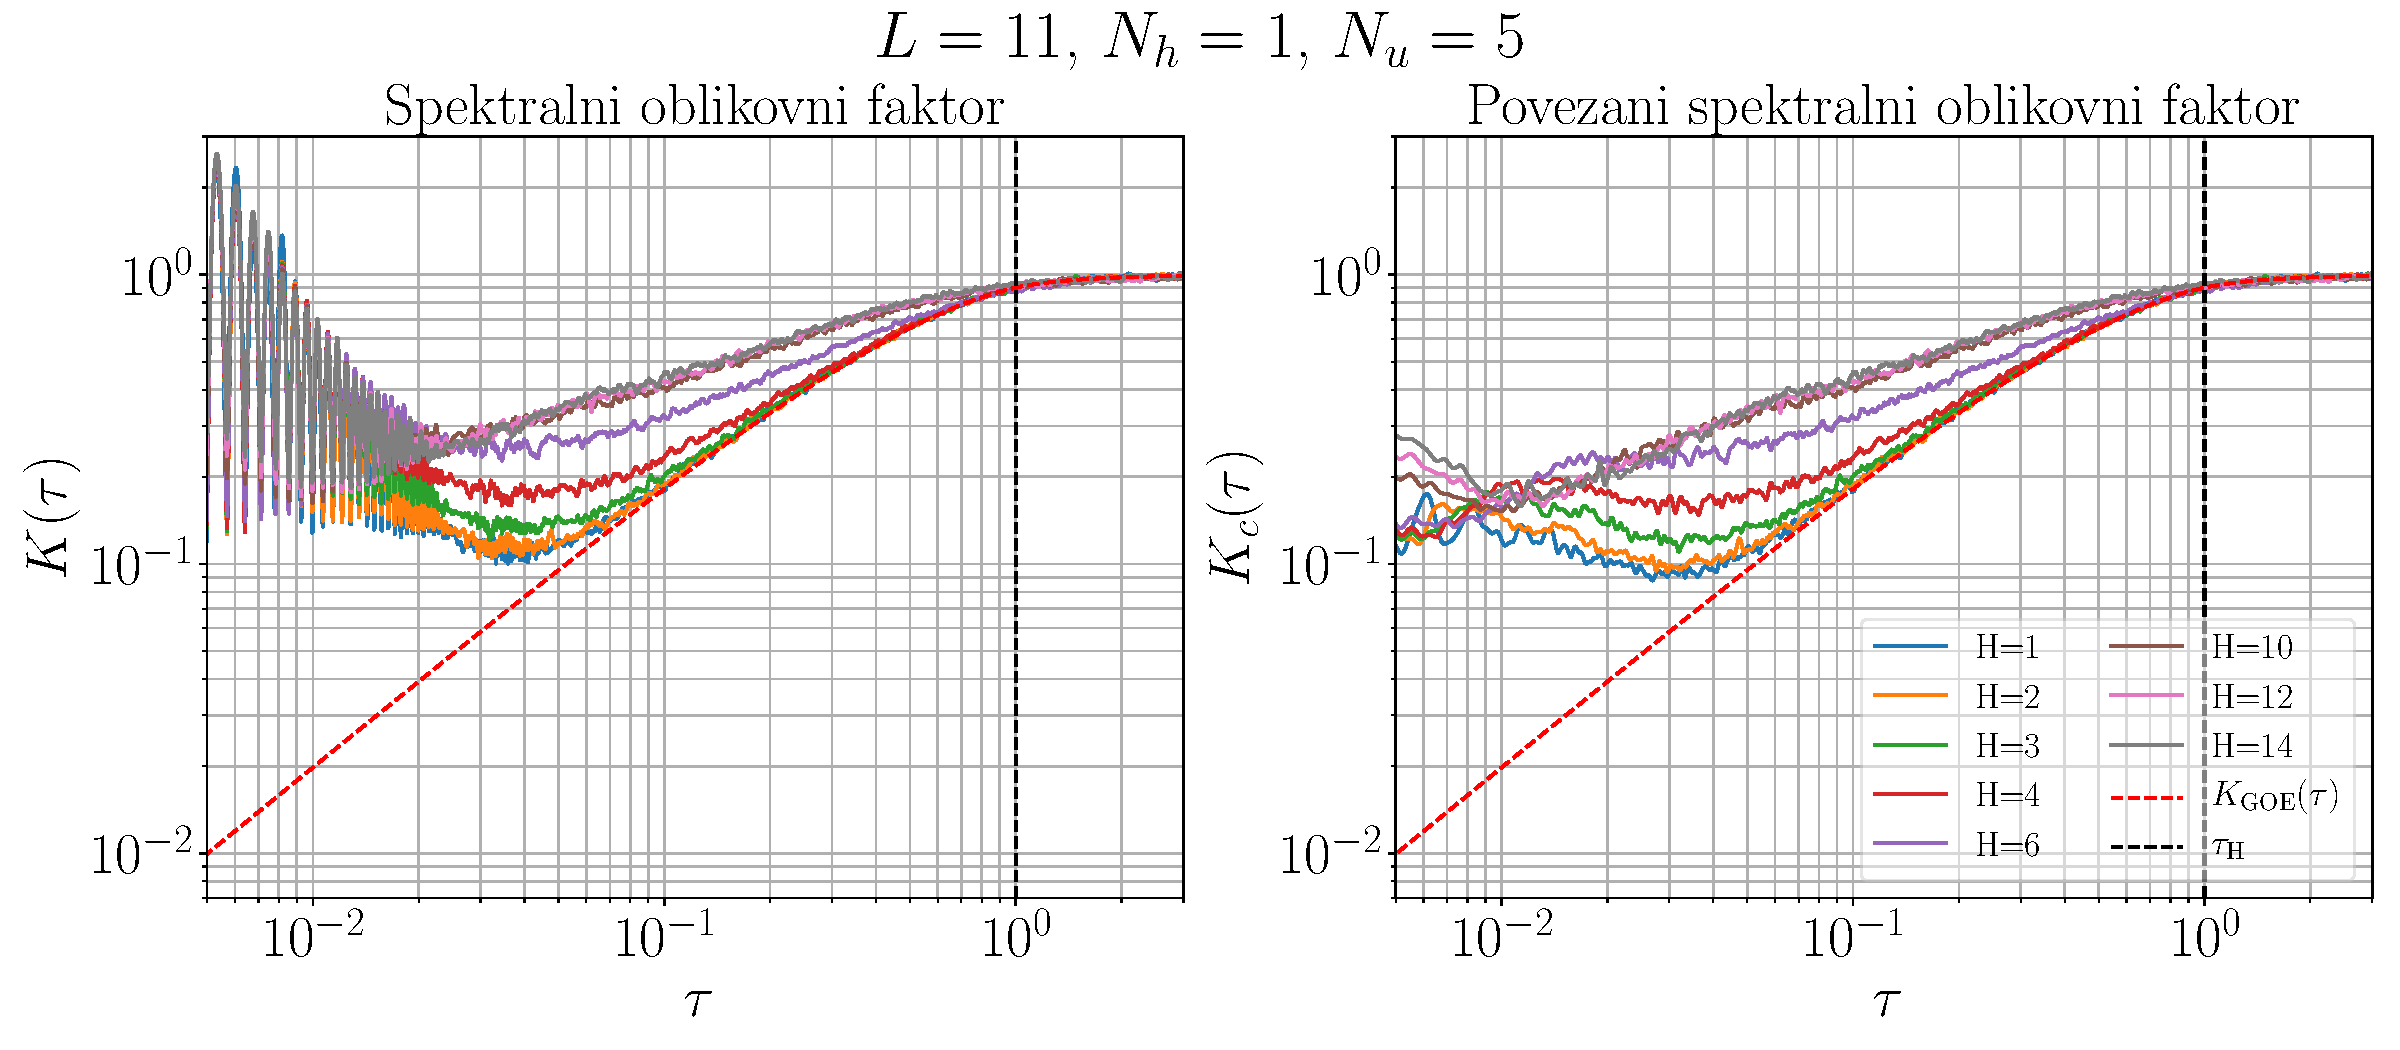
\includegraphics[width=0.93\textwidth]{H_sweep_sff_disorder_11_1_5.pdf}}
\caption{V primeru spreminjanja parametra velikosti potencialnega nereda $H$ so rezultati za dopiranje z eno vrzeljo bistveno drugačni kot pri povečevanju spinskega nereda, saj odvisnost $K(\tau)$ pri preizkušenih vrednostih nikoli ne doseže konstantne vrednosti $K_\mathrm{Poisson}(\tau).$ Krivulje za $H=10$, $H=12$ in $H=14$ sovpadajo, zato se zdi, da potencialni nered ne more povzročiti prehoda v MBL fazo. Ujemanje rezultatov s teoretičnimi napovedmi je podrobneje predstavljeno na Sliki~\ref{fig:double_sweep_sff_disorder_11_1_5_four}. }
\label{fig:H_sweep_sff_disorder_11_1_5}
\end{figure} 
\noindent
Učinka povečevanja spinskega oziroma vrzelnega nereda sta v primeru dopiranja z eno vrzeljo očitno kvalitativno različna. V prvem primeru opazimo prehod med univerzalnim obnašanjem, značilnim za GOE sisteme, in obnašanjem, ki ga opazimo v sistemih s Poissonovo spektralno statistiko. Pri povečevanju potencialnega nereda sicer opazimo odstopanje od napovedane linearne rasti, vendar se rezultati pri preizkušenih vrednostih nereda nikdar ne ujemajo s konstantno vrednostjo $K_\mathrm{Poisson}(\tau).$\\\\
Odstopanje numeričnih izračunov od teoretične napovedi $K_\mathrm{GOE}(\tau)$ smo preverili z izračunom relativnega odstopanja, ki smo ga definirali kot 
\begin{equation}
\Delta K_c(\tau) = \abs{\frac{K_c(\tau) - K_\mathrm{GOE}(\tau)}{K_\mathrm{GOE}(\tau)}}.
\end{equation}
Rezultati so za nekaj vrednosti parametrov $W$ in $H$ v primeru dopiranja z eno vrzeljo prikazani na Sliki~\ref{fig:double_sweep_sff_disorder_11_1_5_four}. 
 \begin{figure}[H]
\centering{
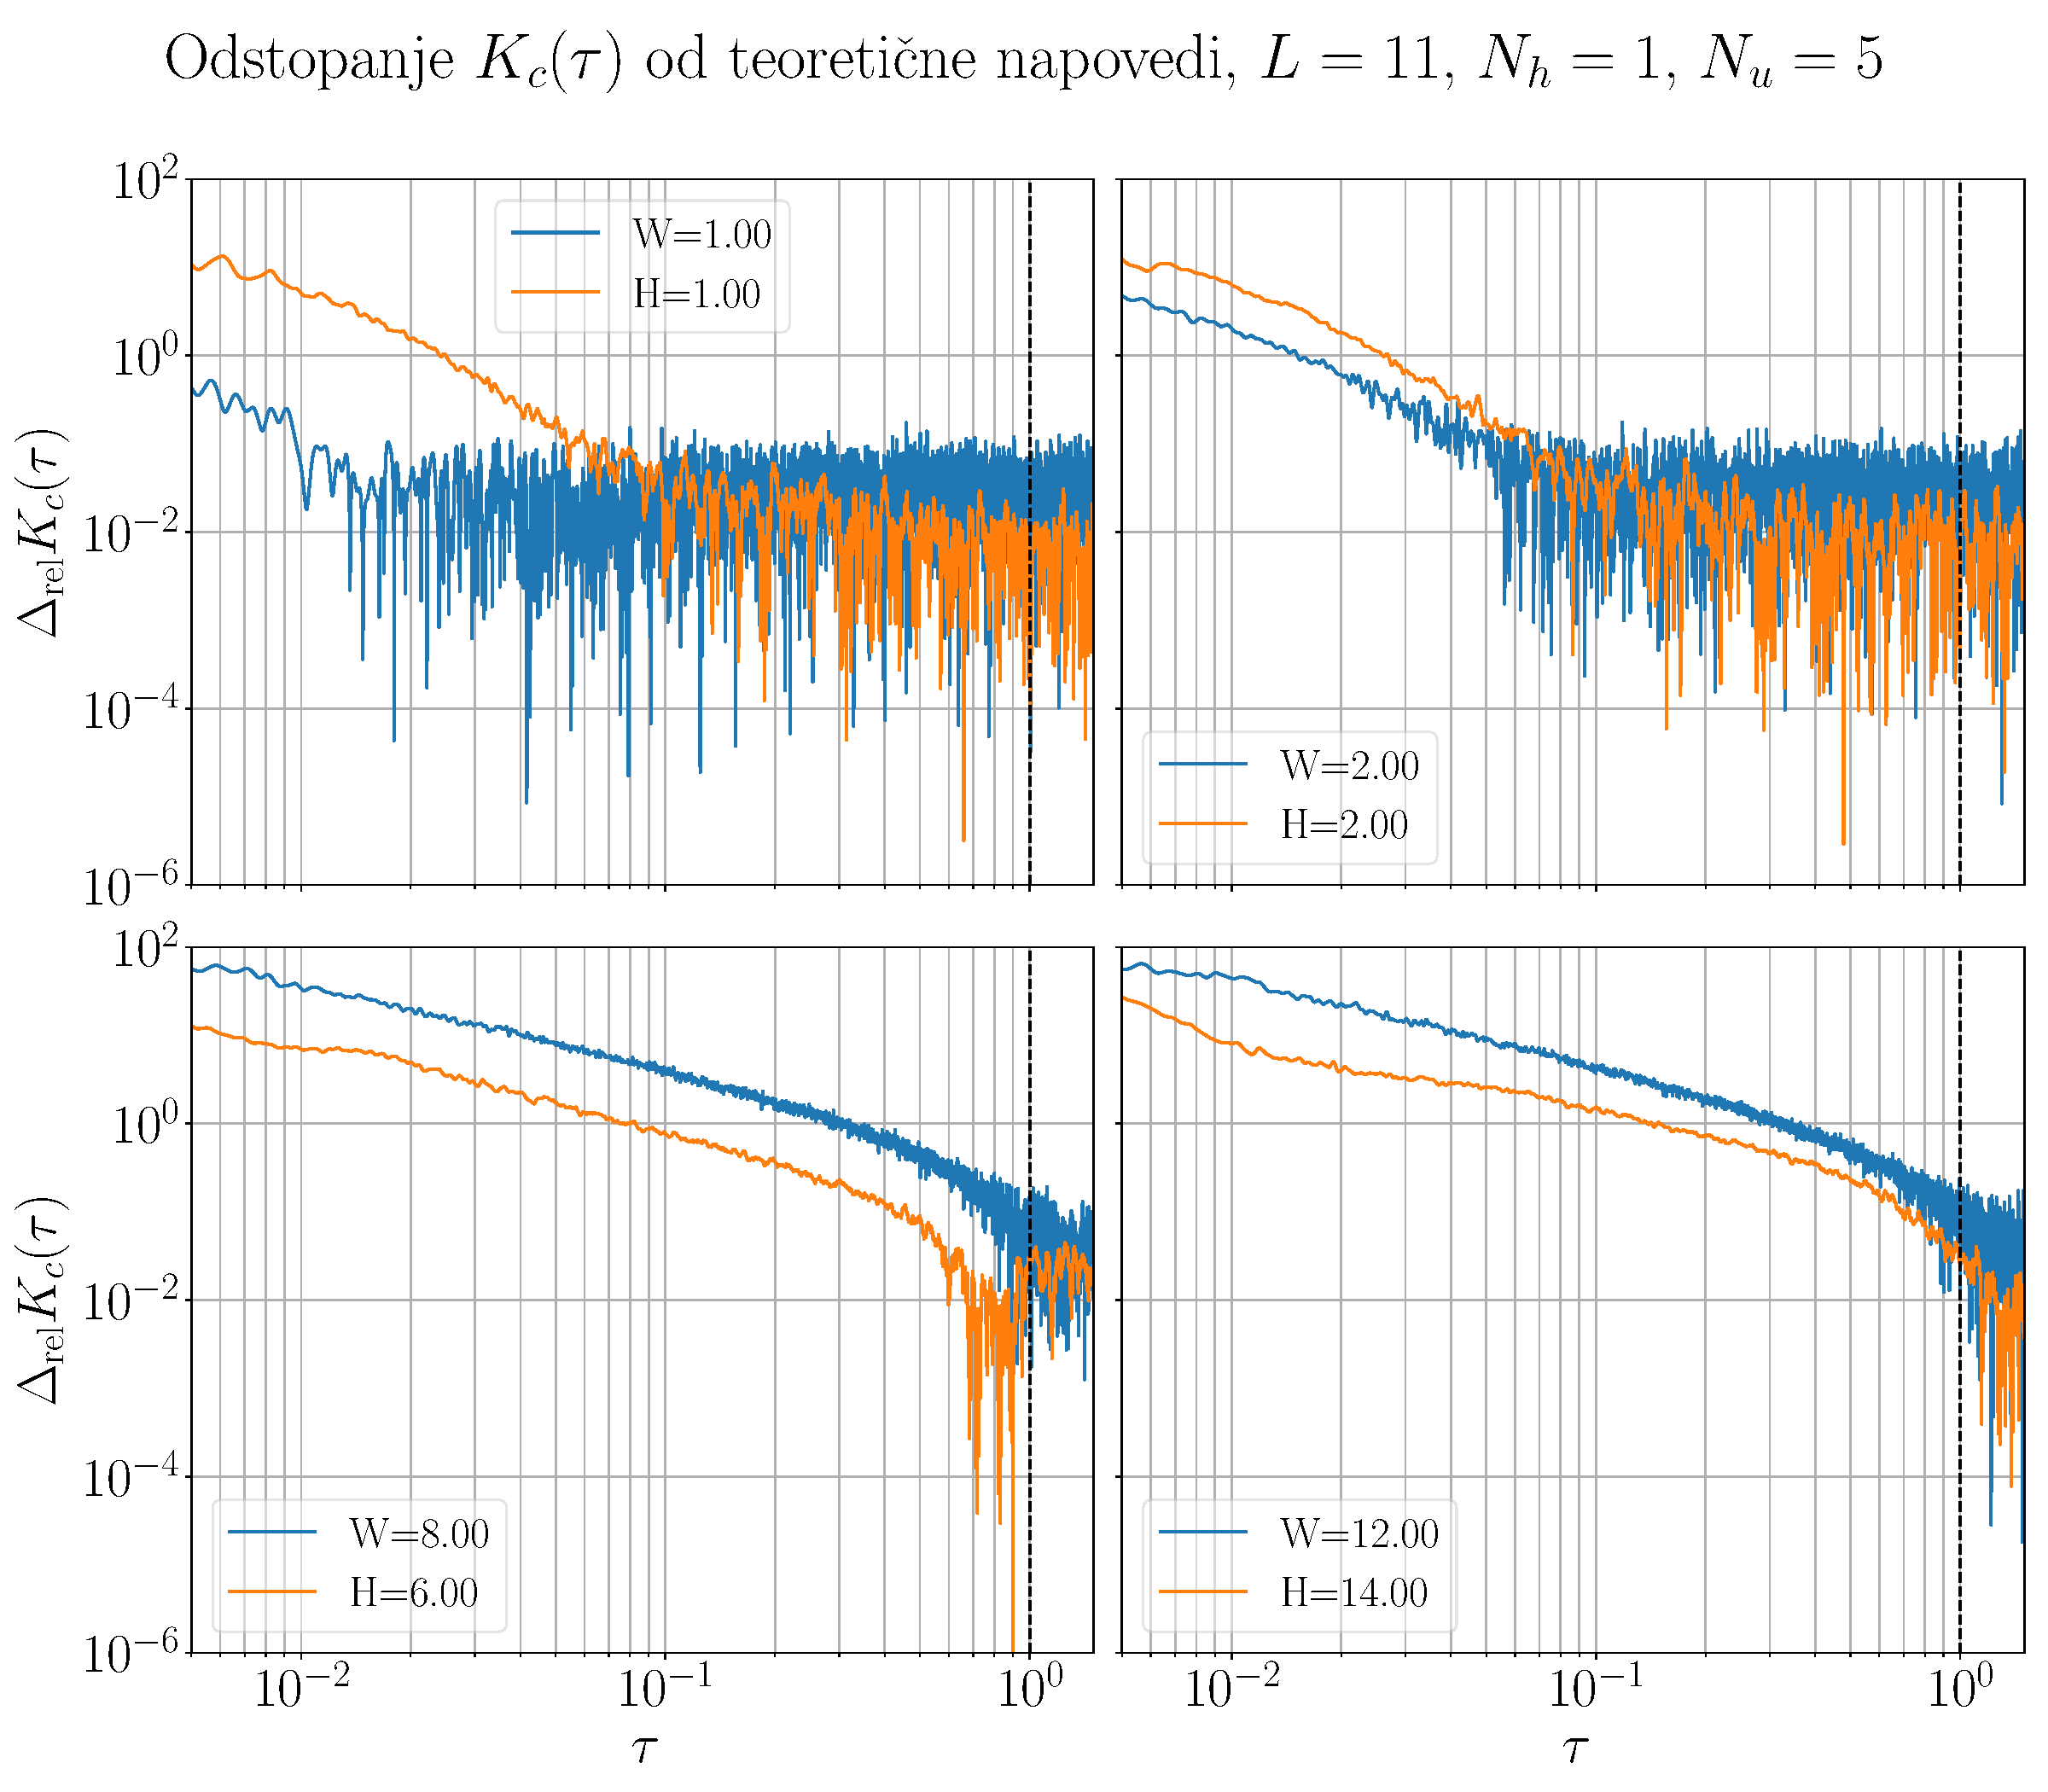
\includegraphics[width=0.85\textwidth]{double_sweep_sff_disorder_11_1_5_four_.pdf}}
\caption{Odstopanje numeričnih izračunov pri nekaj različnih vrednostih parametrov spinskega in potencialnega nereda od teoretične napovedi $K_\mathrm{GOE}(\tau).$ Pri prvih treh vrednostih potencialnega nereda lahko jasno razločimo območje neuniverzalne relaksacije in območje univerzalne linearne rasti, ko se odstopanje ustali in fluktuira okrog povprečne vrednosti. Zgolj na podlagi relativnega odstopanja v mejnih primerih ne moremo presojati ergodičnosti oziroma prisotnosti večdelčne lokalizacije v sistemu, o čemer priča primer pri $H=14.00.$ Relativno odstopanje kaže na odsotnost linearnega naraščanja za $\tau\leq\tau_\mathrm{H},$ vendar izračuni, prikazani na Sliki~\ref{fig:H_sweep_sff_disorder_11_1_5}, nakazujejo, da sistem nima Poissonove spektralne statistike. }
\label{fig:double_sweep_sff_disorder_11_1_5_four}
\end{figure}
\newpage
\noindent	 
V primeru tretjinskega dopiranja spreminjanje velikosti obeh parametrov nereda vodi do prehoda med ergodično in MBL fazo, v skladu z rezultati iz poglavja~\ref{odmik_rezultati}. Za razliko od sistemov z eno vrzeljo je pri tretjinskem dopiranju obnašanje za oba tipa nereda podobno. Numerični izračuni so prikazani na Sliki~\ref{fig:W_sweep_sff_disorder_9_3_3}, primerjava s teoretično napovedjo pa na Sliki~\ref{fig:double_sweep_sff_disorder_9_3_3_four}.
\begin{figure}[H]
\centering{
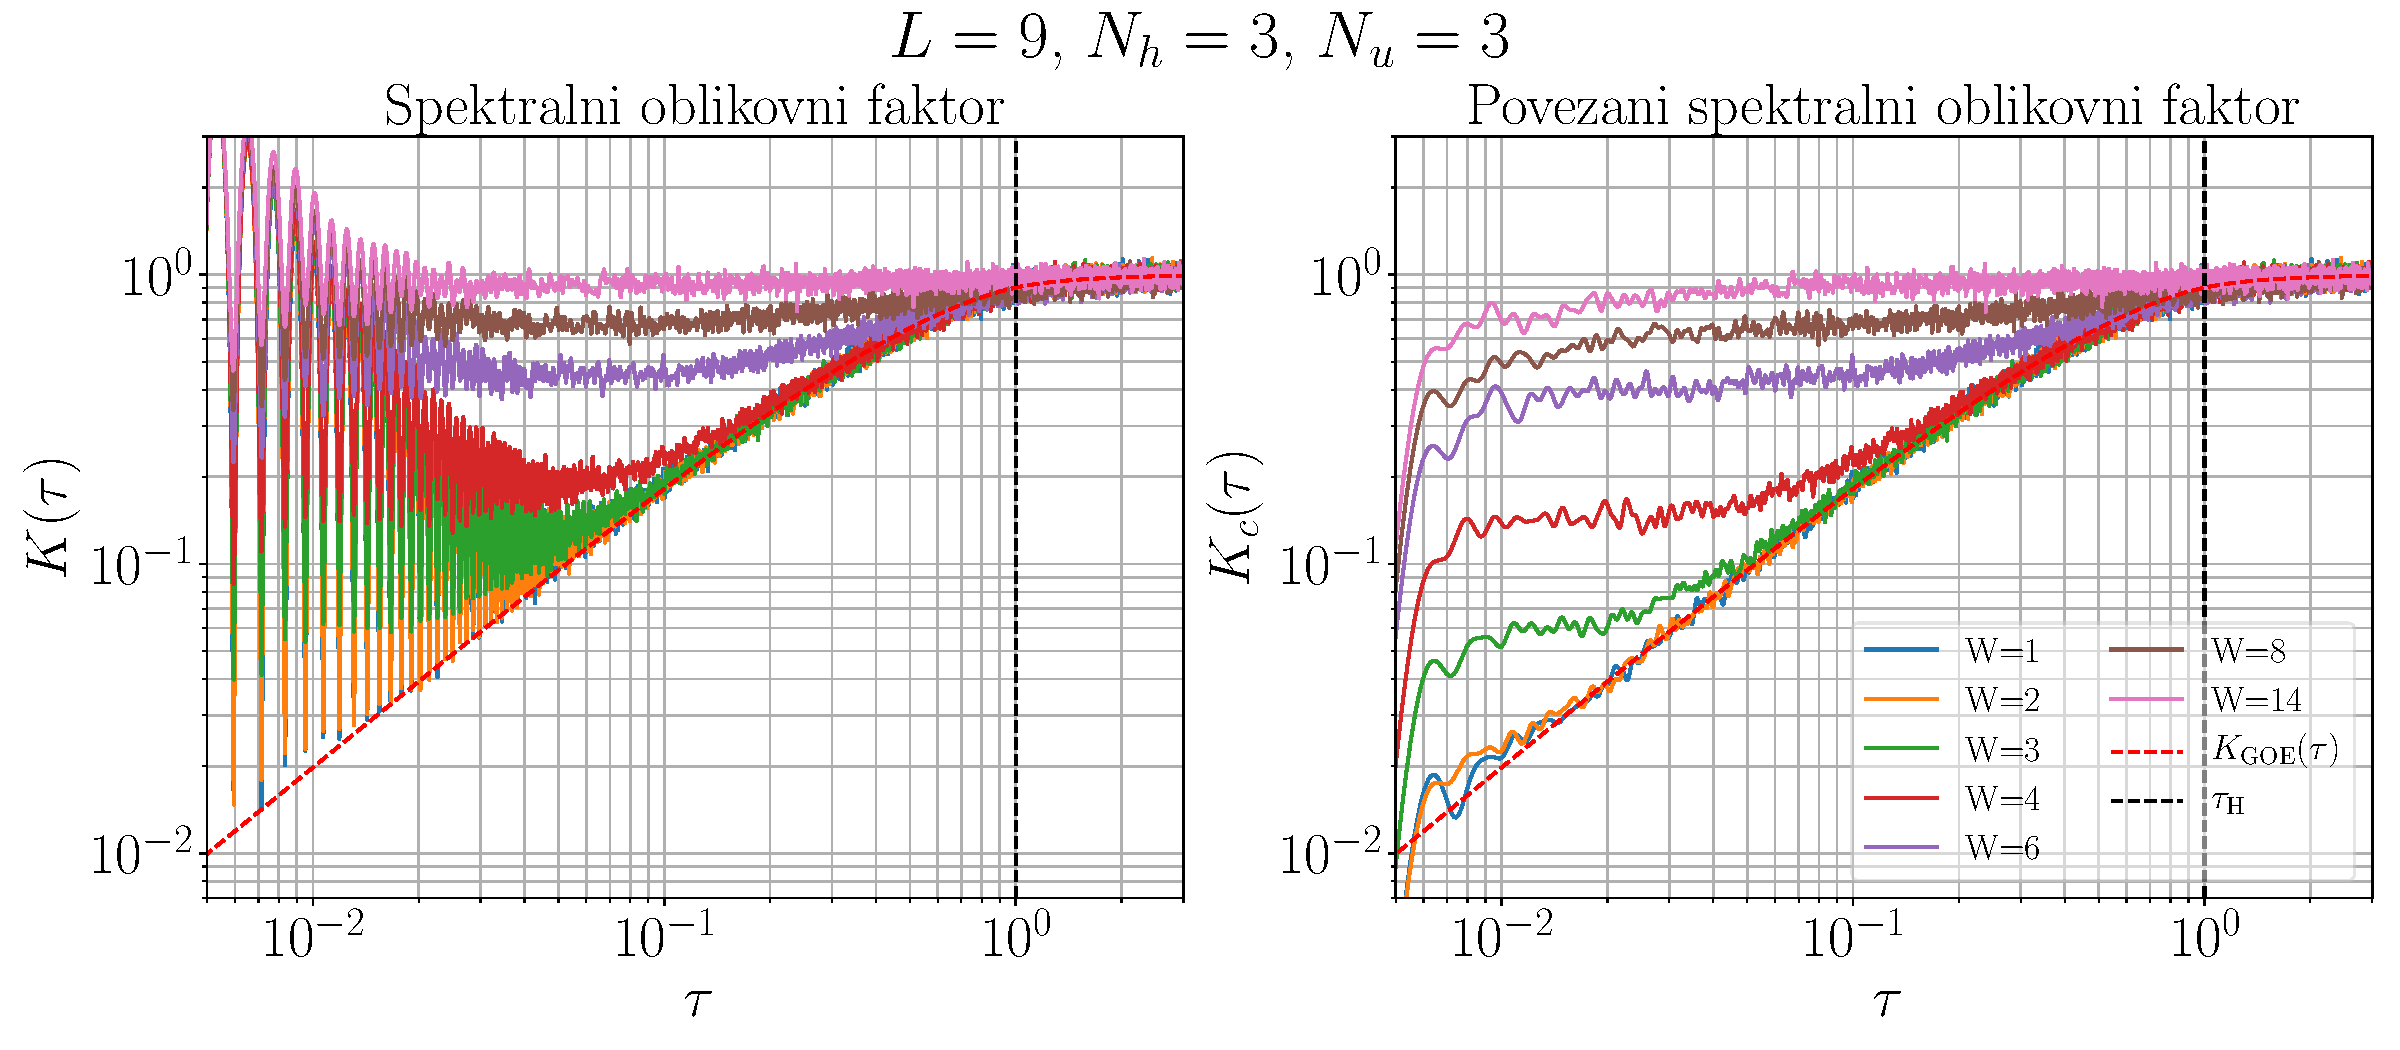
\includegraphics[width=1\textwidth]{W_sweep_sff_disorder_9_3_3.pdf}}
\centering{
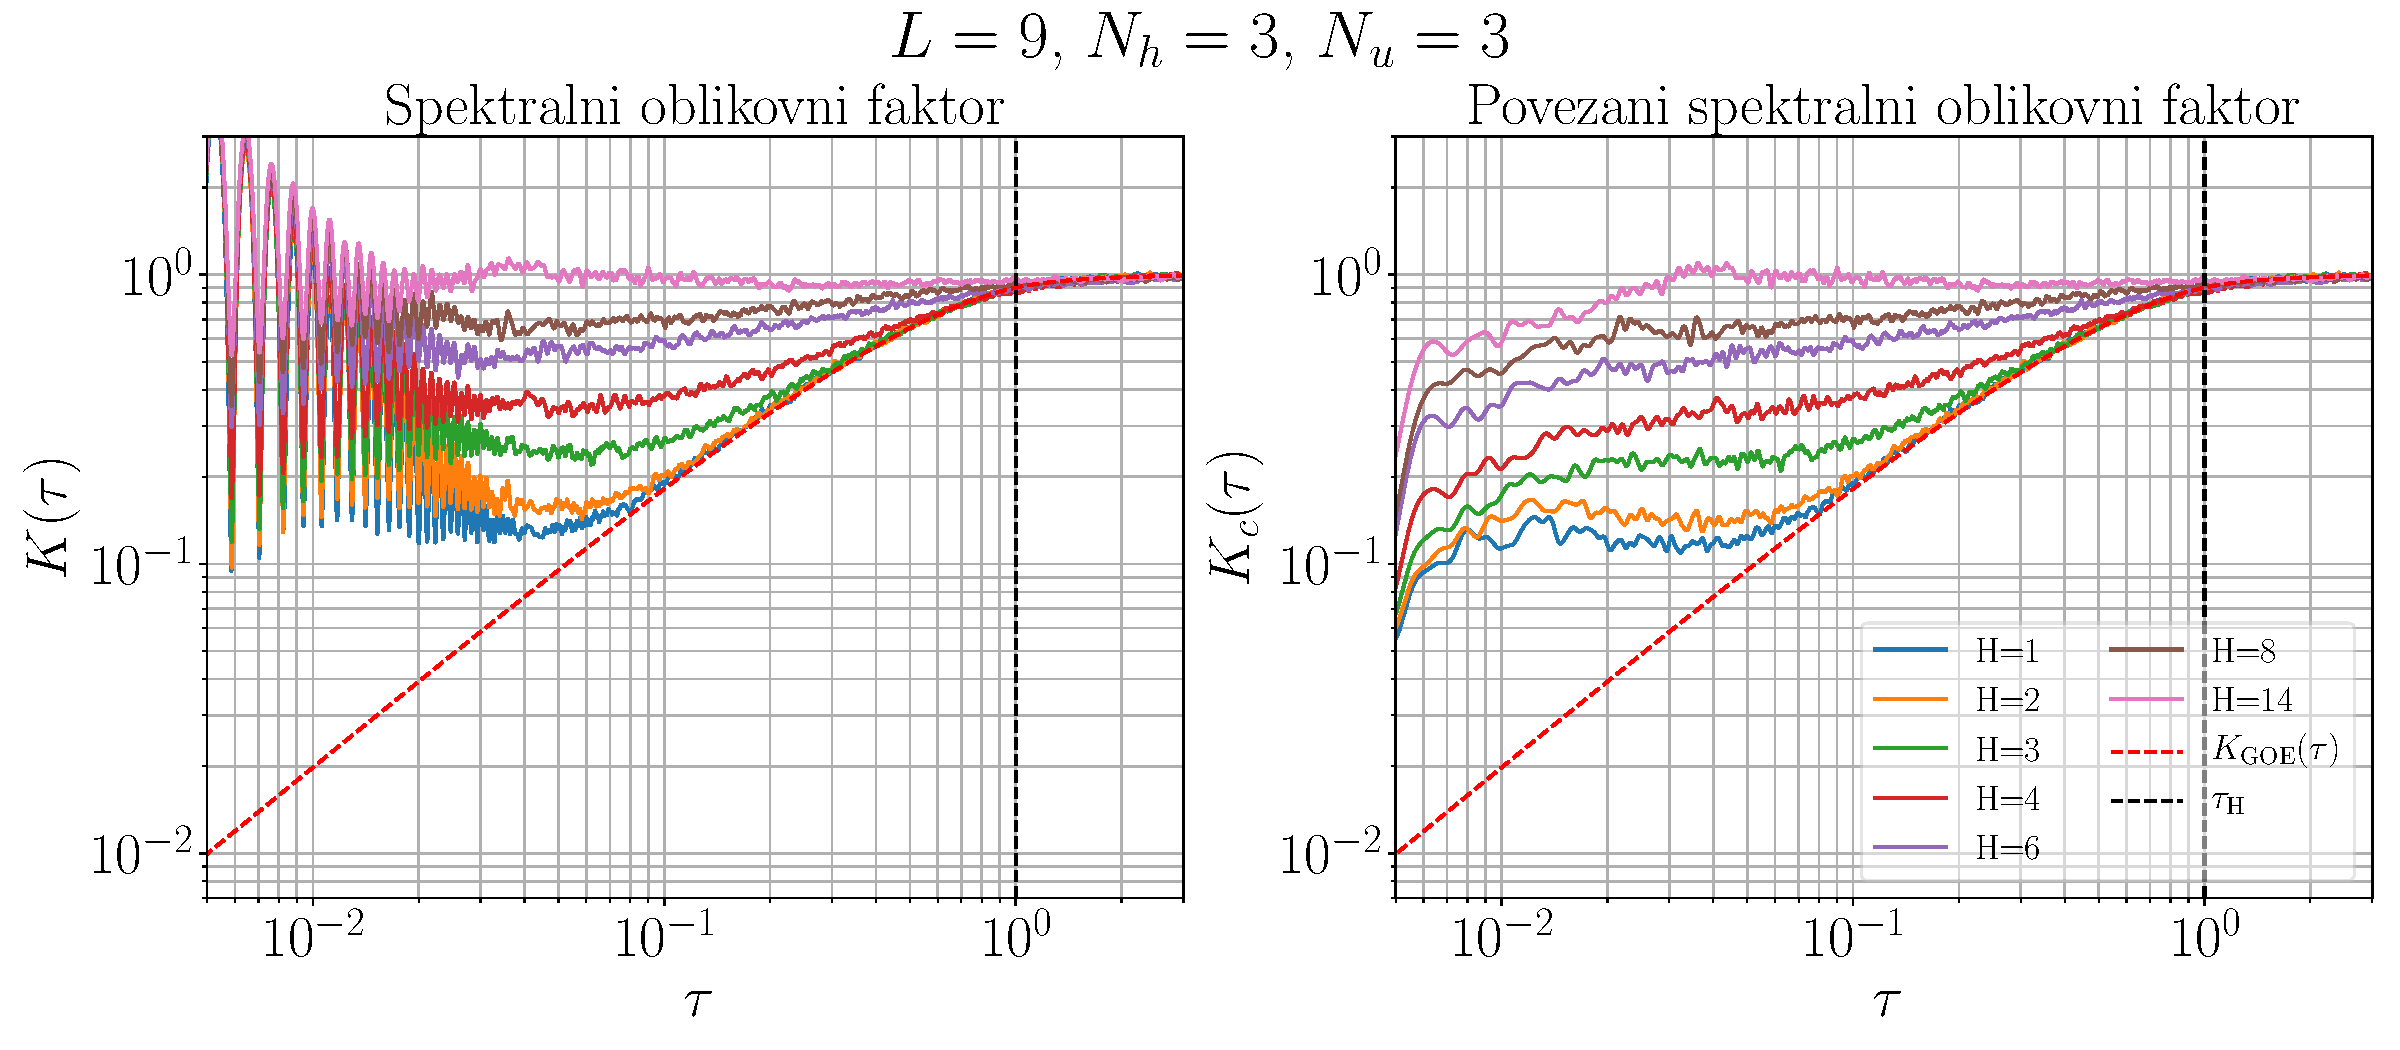
\includegraphics[width=1\textwidth]{H_sweep_sff_disorder_9_3_3.pdf}}
\caption{Zgoraj: izračun $K(\tau)$ in $K_c(\tau)$ pri različnih velikostih parametra spinskega nereda $W$ za primer tretjinskega dopiranja. Povečevanje $W$ vodi do prehoda iz ergodične v MBL fazo. Spodaj: enak izračun, le da za povečevanje parametra potencialnega nereda $H$. Tudi v tem primeru povečevanje parametra vodi do prehoda. V obeh primerih smo izračune dobili s povprečenjem po 500 realizacijah naključnega nereda.  }
\label{fig:W_sweep_sff_disorder_9_3_3}
\end{figure} 
\newpage
%  \begin{figure}[H]
% \centering{
% 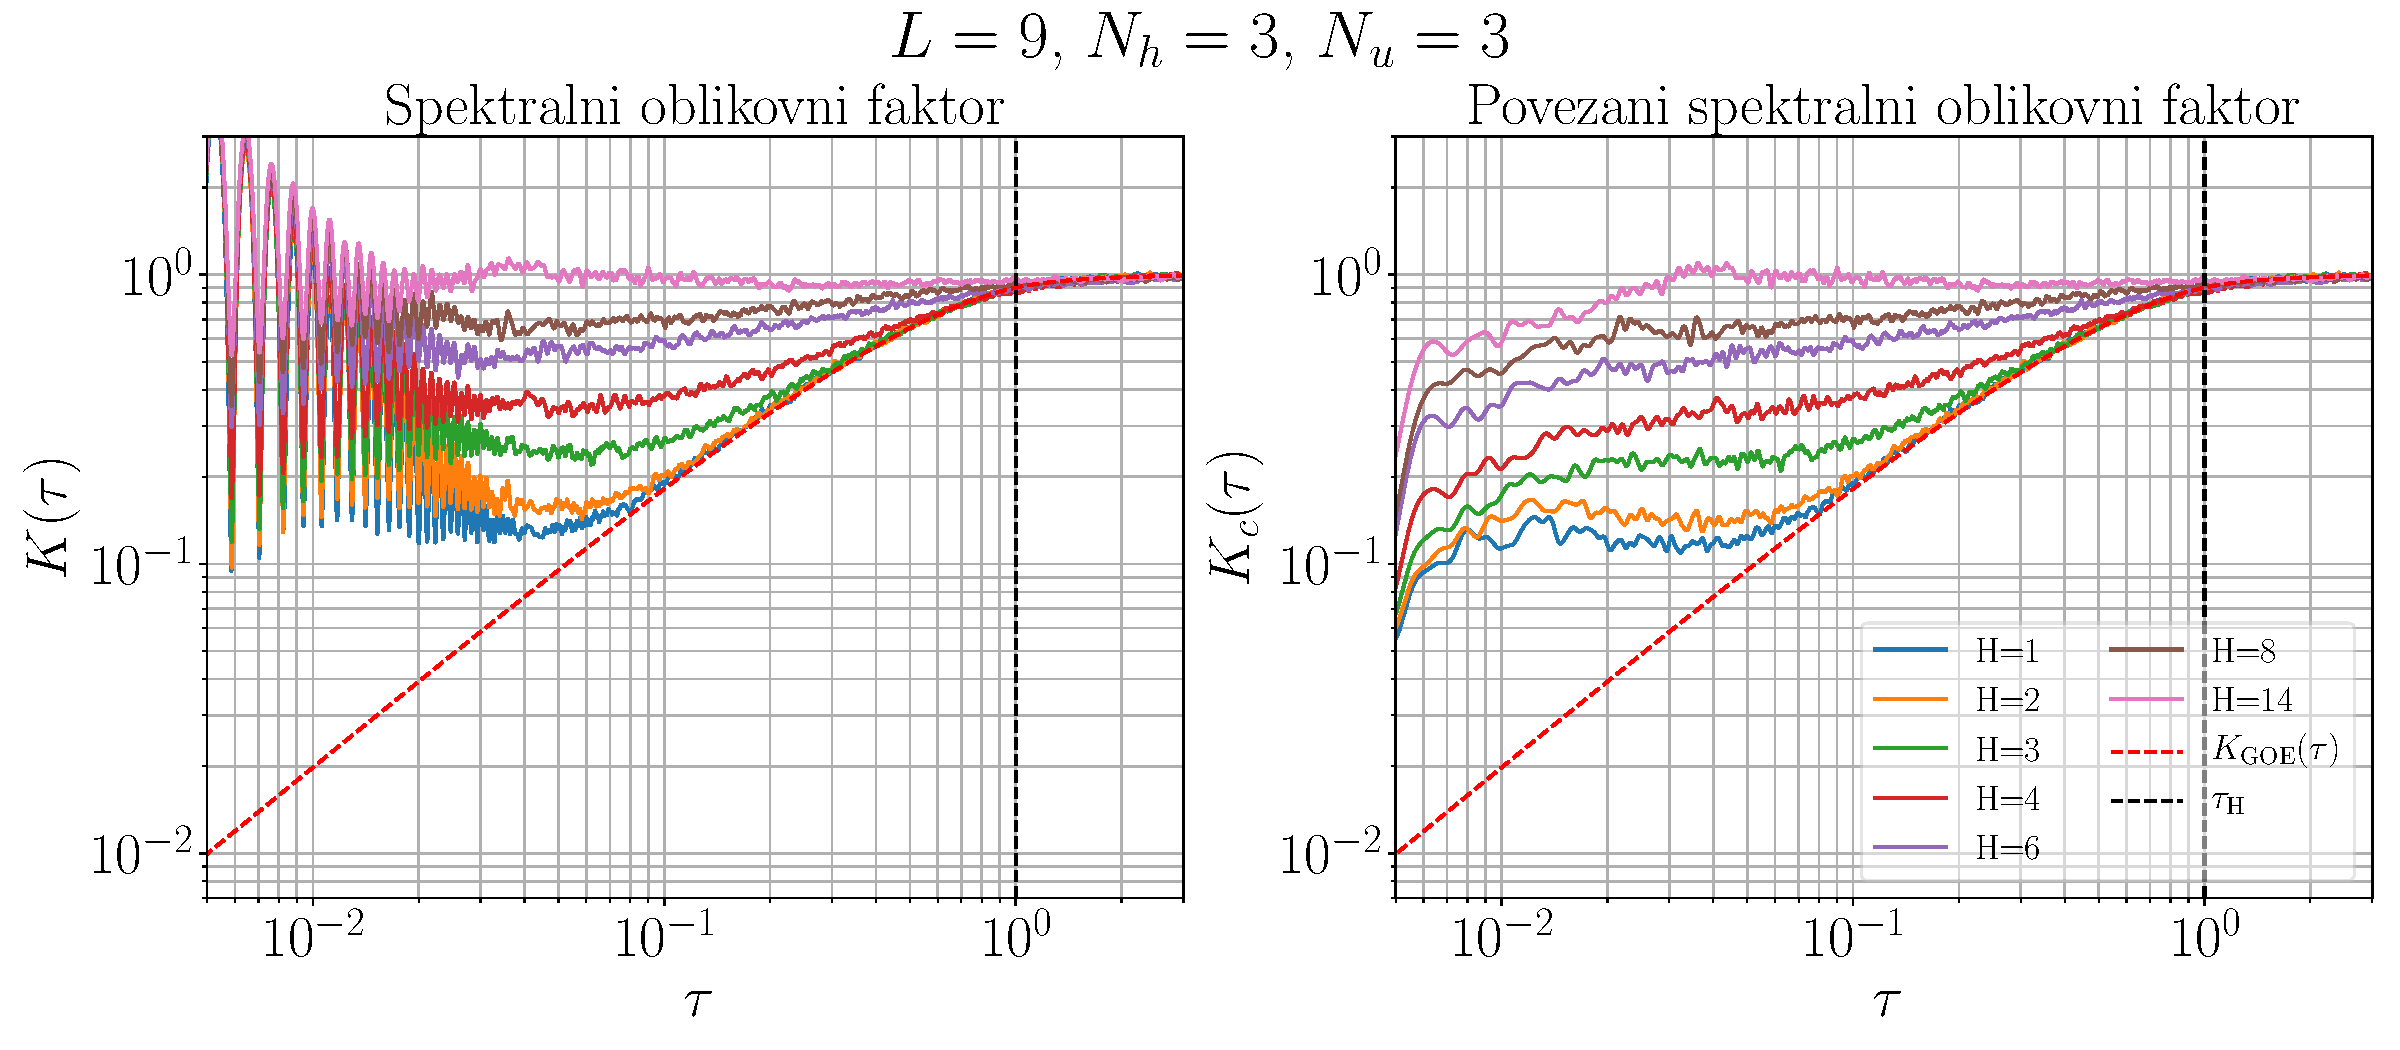
\includegraphics[width=1\textwidth]{H_sweep_sff_disorder_9_3_3.pdf}}
% \caption{}
% \label{fig:H_sweep_sff_disorder_9_3_3}
% \end{figure} 
 \begin{figure}[H]
\centering{
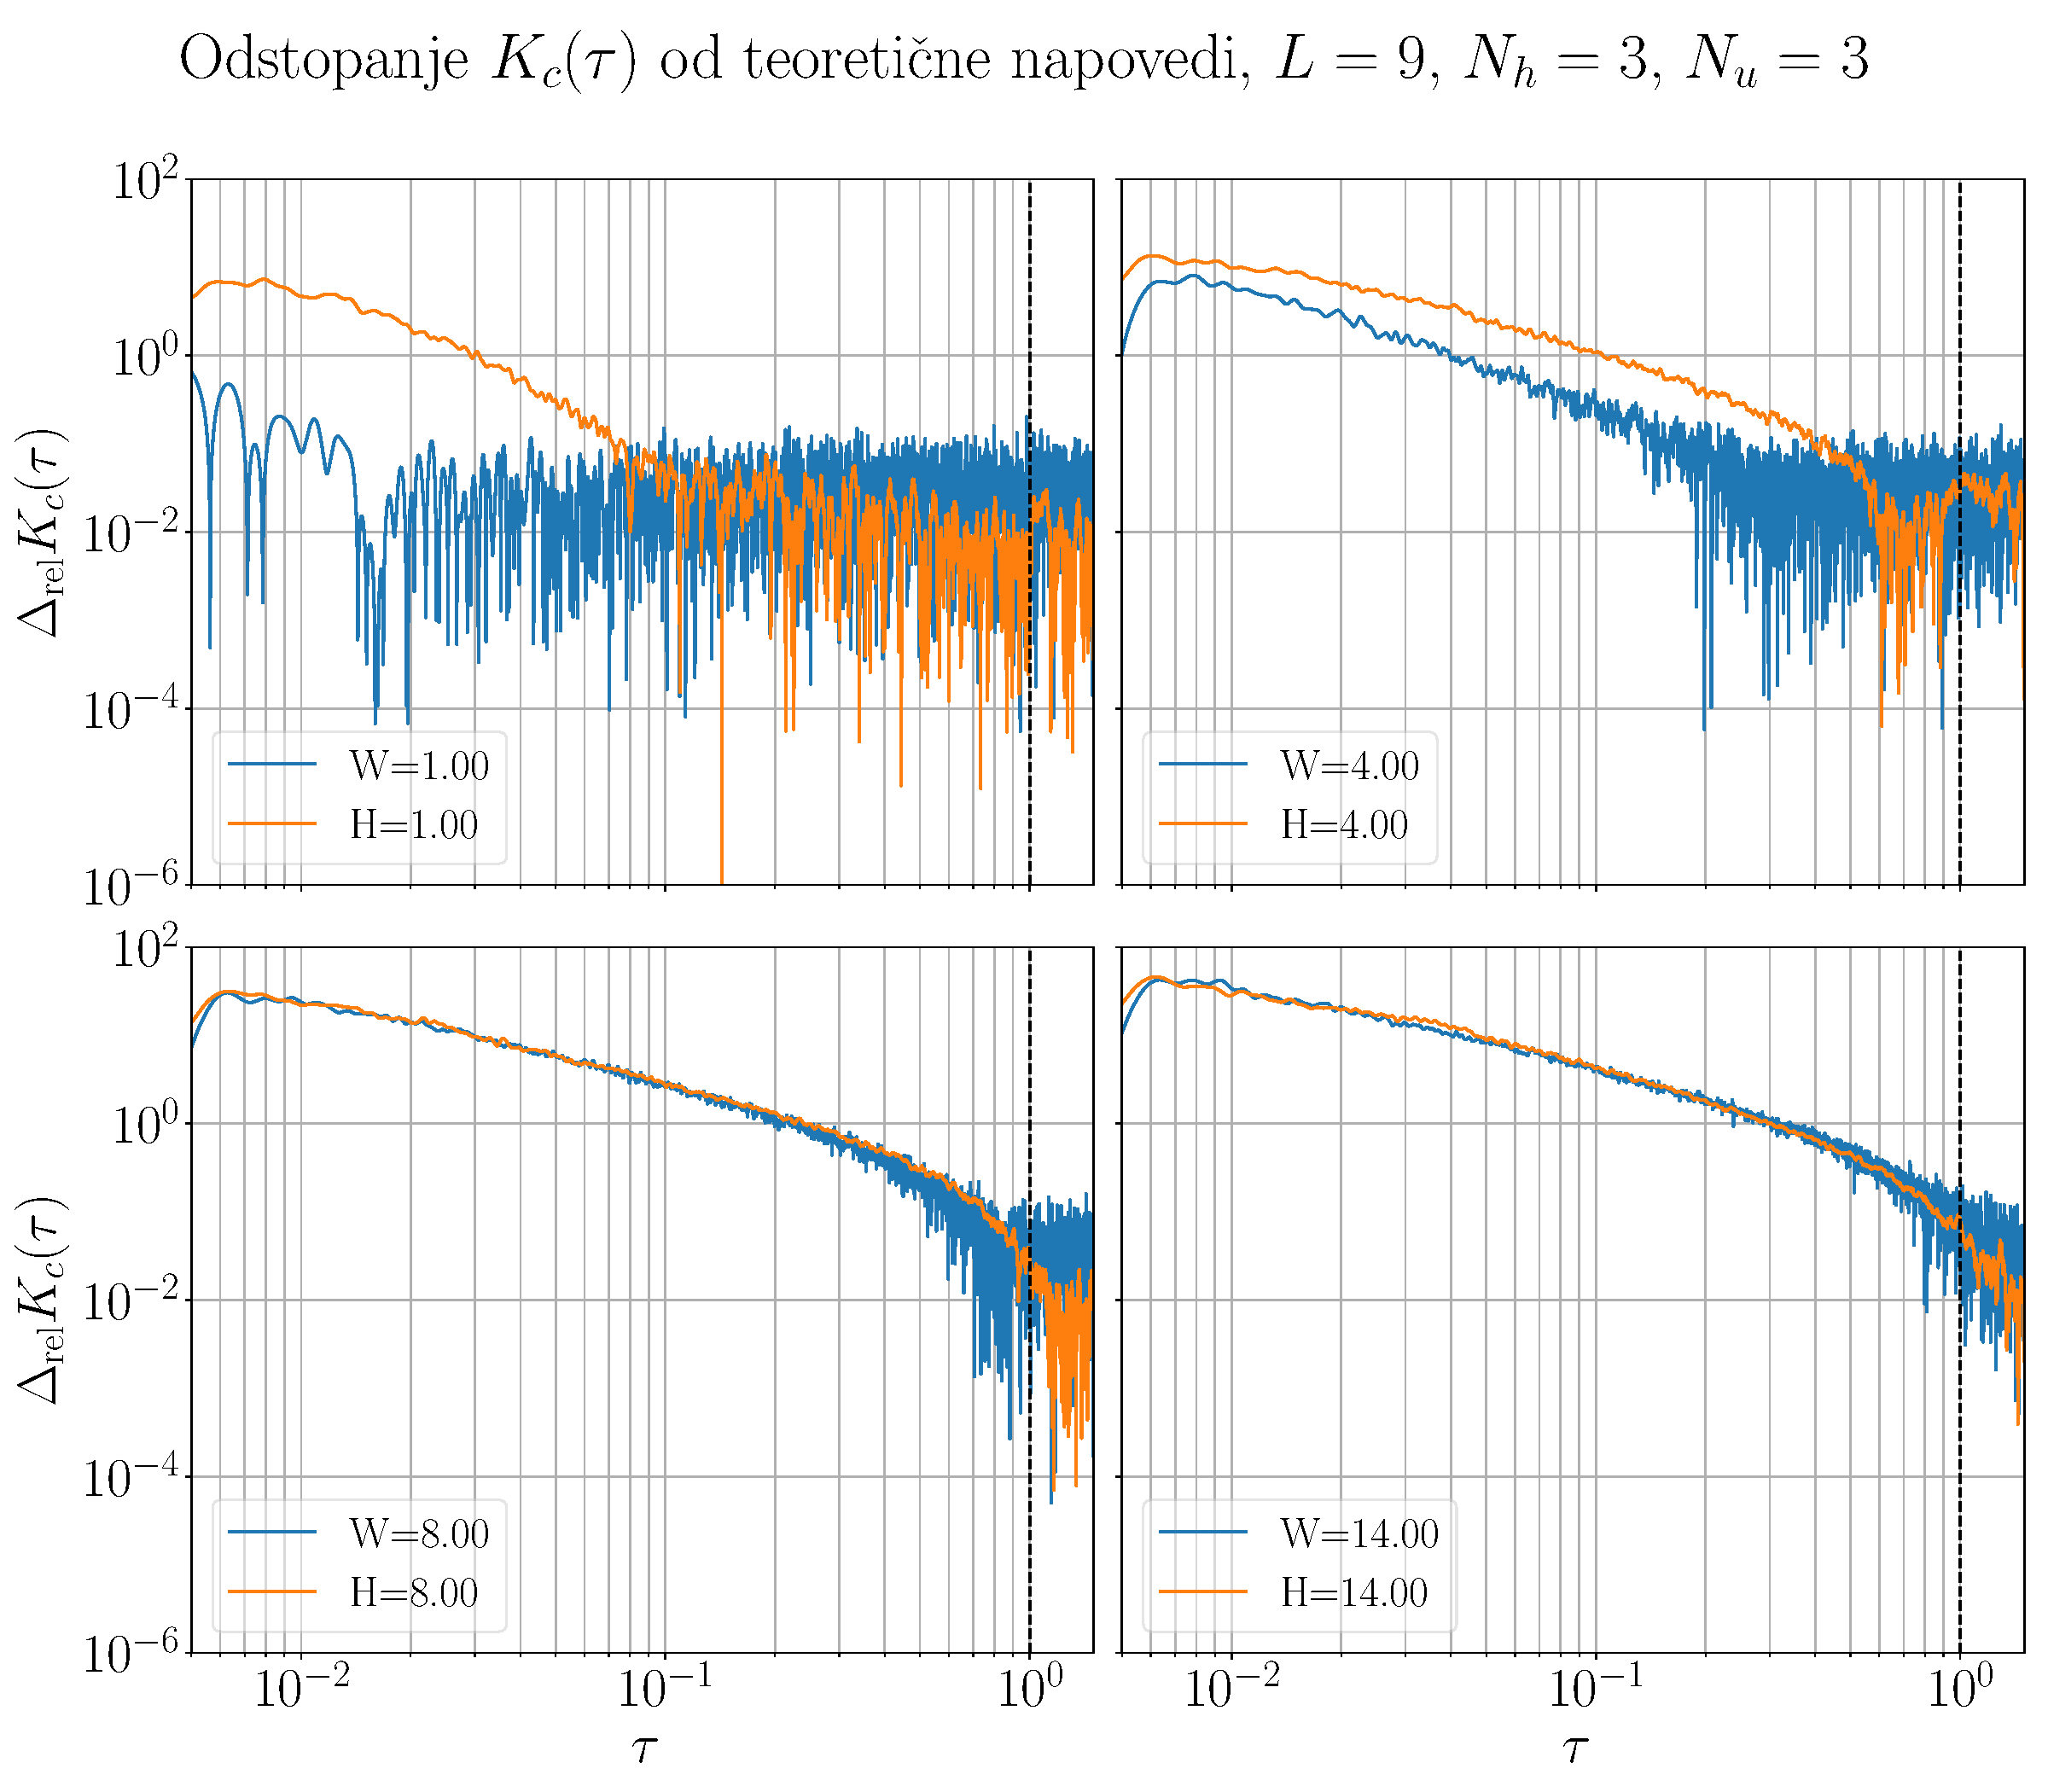
\includegraphics[width=0.85\textwidth]{double_sweep_sff_disorder_9_3_3_four_.pdf}}
\caption{Relativno odstopanje numerično izračunane vrednosti $K_c(\tau)$ od teoretične napovedi $K_\mathrm{GOE}(\tau)$ - enak izračun kot na Sliki~\ref{fig:double_sweep_sff_disorder_11_1_5_four}, le da za primer tretjinskega dopiranja. }
\label{fig:double_sweep_sff_disorder_9_3_3_four}
\end{figure}

\chapter{Prepletenostna entropija}
\label{prepletenostna_numericno}
\section{Vpeljava}
Poleg spektralnih značilnosti smo za presojo ergodičnosti oziroma večdelčne lokaliziranosti sistema analizirali tudi prepletenostno entropijo večdelčnih lastnih stanj. Pri izračunu slednje celoten sistem razdelimo na podsistema A in B. Reducirano gostotno matriko $\rho_\mathrm{A}$ podsistema A dobimo iz gostotne matrike celotnega sistema $\rho$ z izvedbo delne sledi po prostostnih stopnjah podsistema B:
\begin{equation}
\rho_\mathrm{A}=\mathrm{Tr}_\mathrm{B}\ \rho, \hspace{5mm} \Tr{\rho_\mathrm{A}}=1
\end{equation}
Pri izračunih, predstavljenih v magistrski nalogi, smo biparticijo vselej izvedli v realnem prostoru, kjer na diskretni enodimenzionalni verigi dolžine $L$ podsistem A predstavlja $L_\mathrm{A}$ mest, podsistem B pa $L-L_\mathrm{A}$ preostalih mest. Prepletenostna entropija $S_\mathrm{ent}(\mathrm{A})$ je definirana kot von Neumannova entropija podsistema A
\begin{equation}\label{eq:ent_entropy_def}
S_\mathrm{ent}(\mathrm{A})=-\Tr\left\{\rho_\mathrm{A} \log \rho_\mathrm{A}\right\}=-\sum\limits_{i=1}^{d_\mathrm{A}} \lambda_i^\mathrm{A} \log \lambda_i^\mathrm{A},
\end{equation} 
kjer je $\left\{\lambda_i^\mathrm{A}\right\}$ spekter lastnih vrednosti operatorja $\rho_\mathrm{A}$ in
$d_\mathrm{A}$ dimenzija Hilbertovega prostora podsistema A. Pokazati je možno, da sta pri dani biparticiji prepletenostni entropiji podsistemov enaki, torej $S_\mathrm{ent}(\mathrm{A})=S_\mathrm{ent}(\mathrm{B})$~\cite{grassellientanglement}.\\\\ 
\emph{Produktna} stanja lahko zapišemo v obliki produkta stanj $\ket{\phi_1}_\mathrm{A}$ ter $\ket{\phi_2}_\mathrm{B}$ iz podprostorov A in B kot $\ket{\psi}=\ket{\phi_1}_\mathrm{A}\ket{\phi_2}_\mathrm{B}.$ Prepletenostna entropija teh stanj je enaka nič, medtem ko so stanja, ki jih ne moremo zapisati v produktni obliki, \emph{prepletena} in imajo neničelno prepletenostno entropijo. Maksimalna prepletenostna entropija biparticije je enaka logaritmu števila stanj v manjšem izmed podsistemov, $S_\mathrm{ent}^\mathrm{max}(\mathrm{A})=\log\left[\min\left(d_\mathrm{A}, d_\mathrm{B}\right)\right].$ Vrednost $S_\mathrm{ent}^\mathrm{max}(\mathrm{A})$ nastopi, če so v En.~\eqref{eq:ent_entropy_def} vse 
vrednosti $\lambda_i^\mathrm{A}$ enake $1/d^\mathrm{A}.$ \\\\
Za lastna stanja MBL sistemov sta v \emph{celotnem} spektru značilna nizka prepletenost in površinsko skaliranje prepletenostne entropije. Slednje pomeni, da v limiti $L\to\infty$ velja $S_\mathrm{ent}(\mathrm{A})/L\to0$. Če povečujemo velikost sistema in pri tem ohranjamo konstantno razmerje $L_\mathrm{A}/L,$ potem prepletenostna entropija skalira sorazmerno z volumnom roba podsistema, $S_\mathrm{ent}(\mathrm{A})\propto\mathrm{vol}\left(\delta A\right).$ Ta je v eni dimenziji konstanten, $\mathrm{vol}\left(\delta A\right)=\mathrm{konst}.$ Na drugi strani sta v ergodičnih sistemih za visoko vzbujena stanja značilni visoka prepletenost in volumsko skaliranje prepletenostne entropije. V tem primeru v limiti $L\to\infty$ velja $S_\mathrm{ent}(\mathrm{A})/L=\mathrm{const.}$ Primera volumskega in površinskega skaliranja prepletenostne entropije sta prikazana na Sliki~\ref{fig:W_sweep_ent_entropy_scaling_systems_14_0_7}, in sicer za model $t$-$J$ brez vrzeli na $L=14$ mestih, ki ustreza izotropnemu Heisenbergovemu modelu, podanem z En.~\eqref{eq:XXZ} pri $J=1$ in $\Delta=1.$
\begin{figure}[H]
\centering{
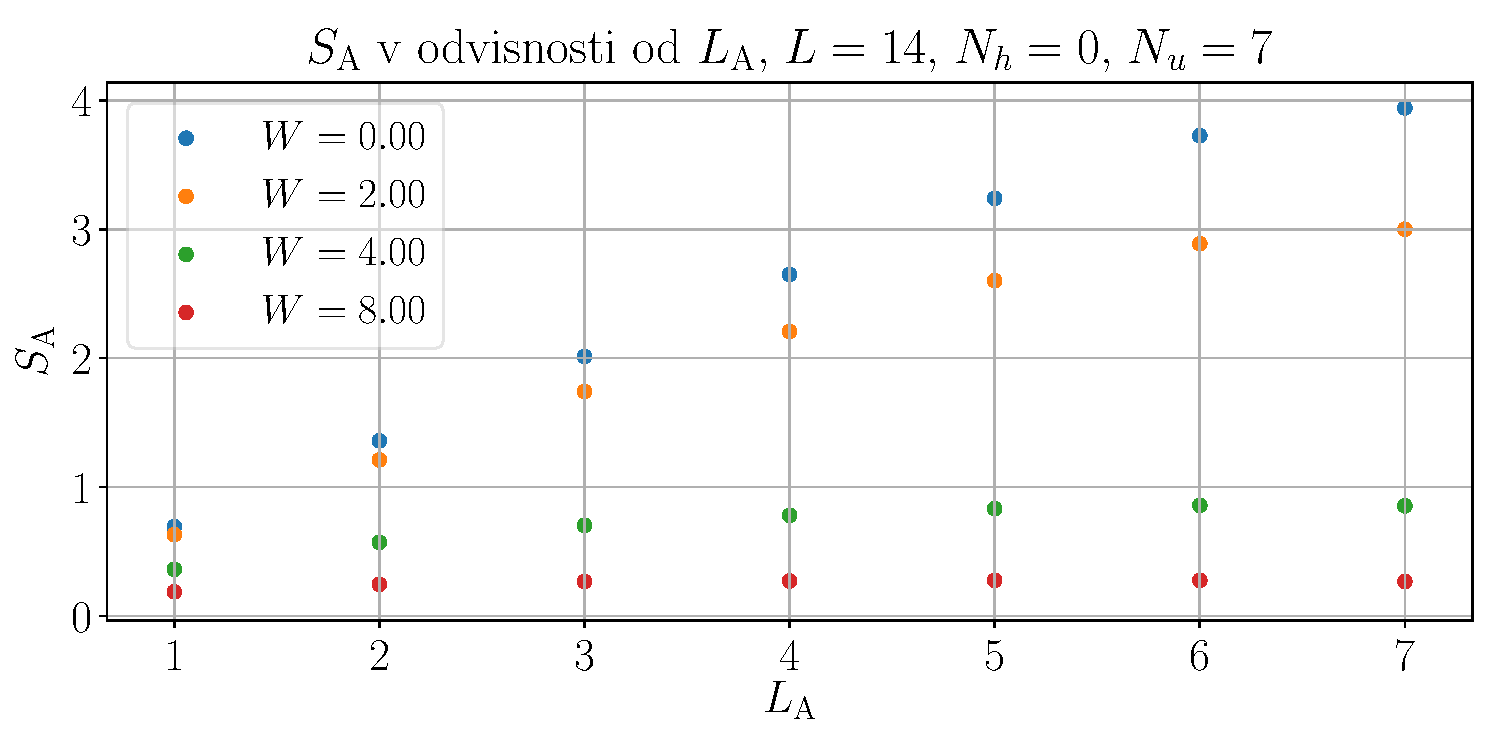
\includegraphics[width=0.7\textwidth]{W_sweep_ent_entropy_scaling_14_0_7.pdf}}
\centering{
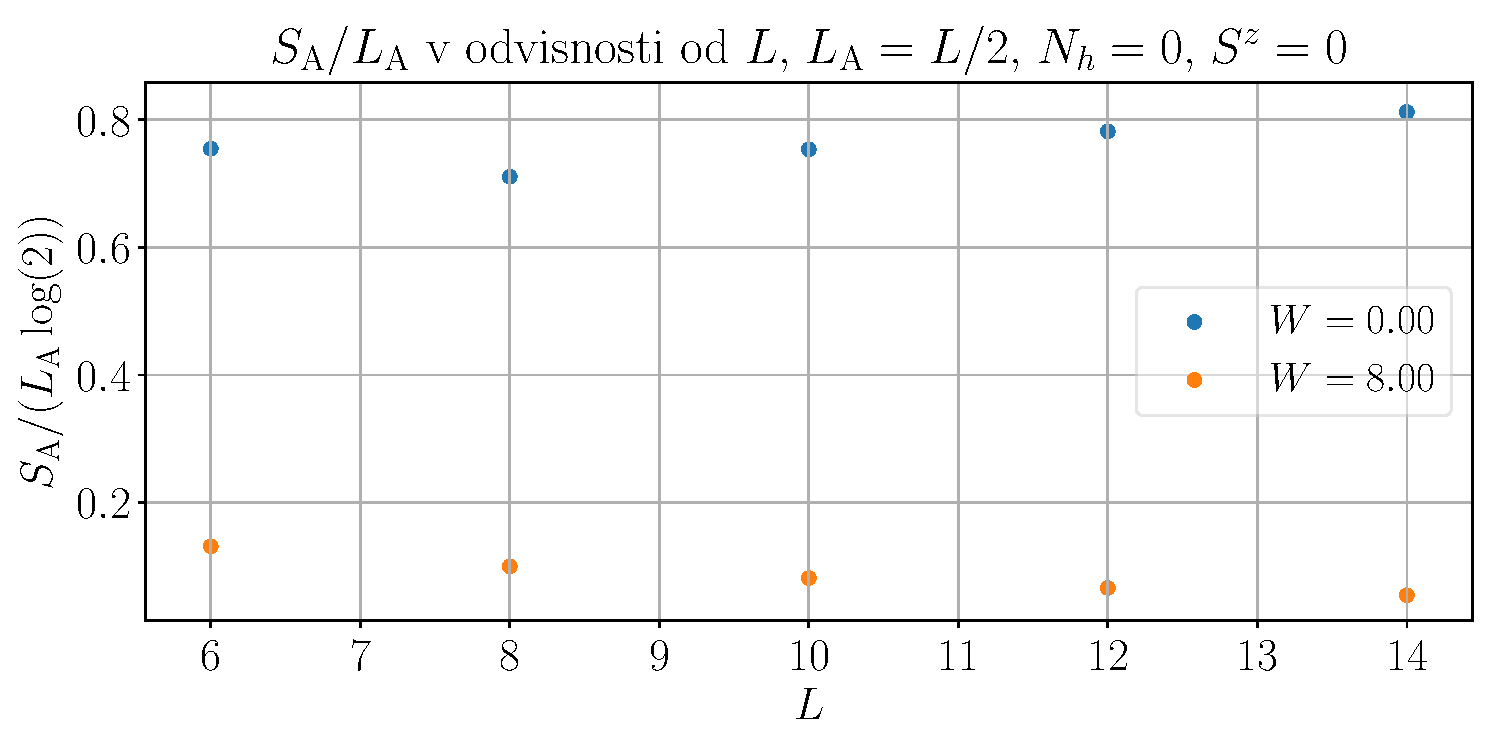
\includegraphics[width=0.7\textwidth]{W_sweep_ent_entropy_scaling_systems_14_0_7.pdf}}
\caption{Prikaz volumskega in površinskega skaliranja prepletenostne entropije $S_\mathrm{A}$ lastnih stanj sistema. Predstavljene so povprečne vrednosti prepletenostne entropije za lastna stanja v sredini pasu.
Zgoraj: odvisnost prepletenostne entropije od velikosti podsistema $L_\mathrm{A}$ pri fiksni velikosti sistema $L$. Pri volumskem skaliranju $S_\mathrm{A}$ v termodinamski limiti neskončnega sistema narašča sorazmerno z $L_\mathrm{A}$, v primeru površinskega skaliranja pa je $S_\mathrm{A}$ v eni dimenziji za vse velikosti podsistemov enak konstanti. Spodaj: skaliranje prepletenostne entropije pri biparticiji na dva enaka podsistema v odvisnosti od velikosti sistema $L$. V limiti $L\to\infty$ velja v primeru volumskega skaliranja $S_\mathrm{A}/L=\mathrm{const.}$, v primeru površinskega skaliranja pa $S_\mathrm{A}/L=0.$ Izračune smo izvedli za model $t$-$J$ brez vrzeli, ki ustreza izotropnemu Heisenbergovemu modelu z $J=1$ z dodatkom nereda. Kot nakazujejo numerične študije, nastopi prehod med ergodično in MBL fazo  v okolici $W=3.5$~\cite{pal2010many}~\cite{luitz2015many}.}
\label{fig:W_sweep_ent_entropy_scaling_systems_14_0_7}
\end{figure}  
\newpage
\section{Rezultati}
Predstavljeni so rezultati izračuna prepletenostne entropije vseh lastnih stanj sistema za model $t$-$J$ z dodatkom različnih tipov nereda, pri čemer se pri predstavitvi zgledujemo po Ref.~\cite{luitz2015many}, v kateri je bil izračun narejen za izotropni Heisenbergov model z naključnim spinskim neredom. Za primerjavo so naši rezultati za ta model prikazani na Sliki~\ref{fig:W_ent_entro_density_14_7_0}. Pri dani velikosti parametra nereda smo prepletenostno entropijo vseh lastnih stanj izračunali pri različnih realizacijah nereda. Interval lastnih energij smo normalizirali na območje med 0 in 1, in sicer po predpisu 
\begin{equation}
\varepsilon=\frac{E-E_\mathrm{min}}{E_\mathrm{max}-E_\mathrm{min}}.
\end{equation}
Pri tem je $E$ energija nekega večdelčnega lastnega stanja, $E_\mathrm{min}$ in $E_\mathrm{max}$ pa najmanjša oziroma največja lastna vrednost v vseh spektrih, izračunanih pri različnih realizacijah nereda. Za različne velikosti parametra nereda so vrednosti $E_\mathrm{min}$ oziroma $E_\mathrm{max}$ različne. Pri posamezni realizaciji nereda smo interval normaliziranih energij $\varepsilon$ razdelili na enake podintervale in v vsakem izmed njih izračunali povprečno vrednost prepletenostne entropije, nato pa smo tako izračunane vrednosti še povprečili po različnih realizacijah nereda. V magistrski nalogi predstavljeni rezultati so bili izračunani s povprečenjem po 500 realizacijah nereda. Ker prepletenostna entropija za stanja, degenerirana v okviru natančnosti točne diagonalizacije, ni dobro definirana, smo z lokalnim zlomom simetrije (glej poglavje~\ref{lokalni_zlom_simetrije}) poskrbeli za odsotnost degeneracij tudi v čistem primeru brez nereda.
Poleg že omenjenega Heisenbergovega modela so na Slikah~\ref{fig:W_ent_entro_density_11_5_1}-~\ref{fig:H_ent_entro_density_9_3_3} prikazani rezultati za model $t$-$J$ v primeru dopiranja z eno vrzeljo oziroma v primeru tretjinskega dopiranja za oba tipa nereda.
% \newpage
% V MBL sistemih so namreč \emph{vsa} lastna stanja v spektru šibko prepletena in njihova prepletenostna entropija $S_\mathrm{A}$, ki jo vpeljemo spodaj, skalira površinsko. To pomeni, da v limiti $L\to\infty,$ velja  $S_\mathrm{A}/L\to0,$ kjer je $L$ velikost sistema. Na drugi strani so v ergodičnih sistemih visoko vzbujena stanja tipično močno prepletena in njihova prepletenostna entropija skalira volumsko 
% \begin{minipage}[t]{0.7\textwidth}
% \begin{figure}[H]
% \centering{
% 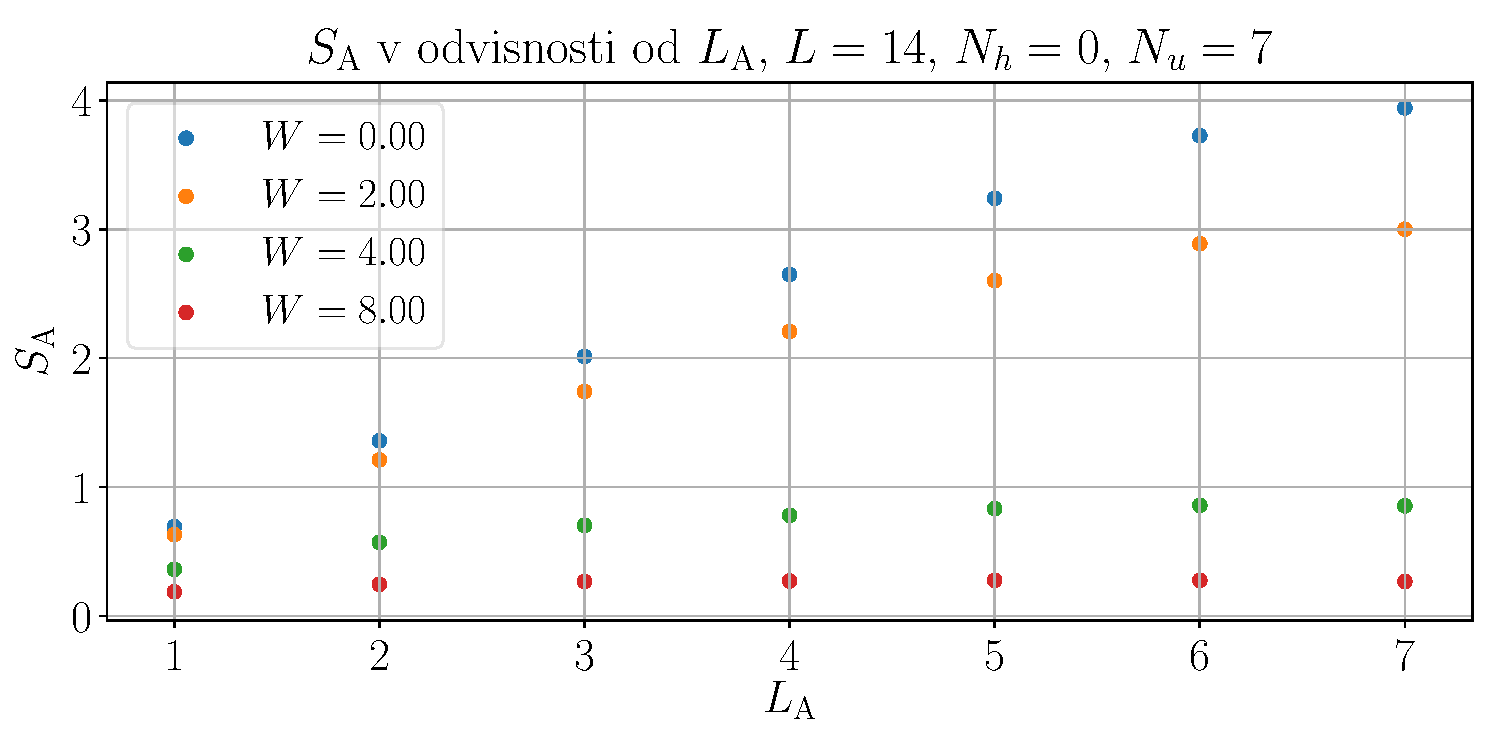
\includegraphics[width=0.7\textwidth]{W_sweep_ent_entropy_scaling_14_0_7.pdf}}
% \centering{
% 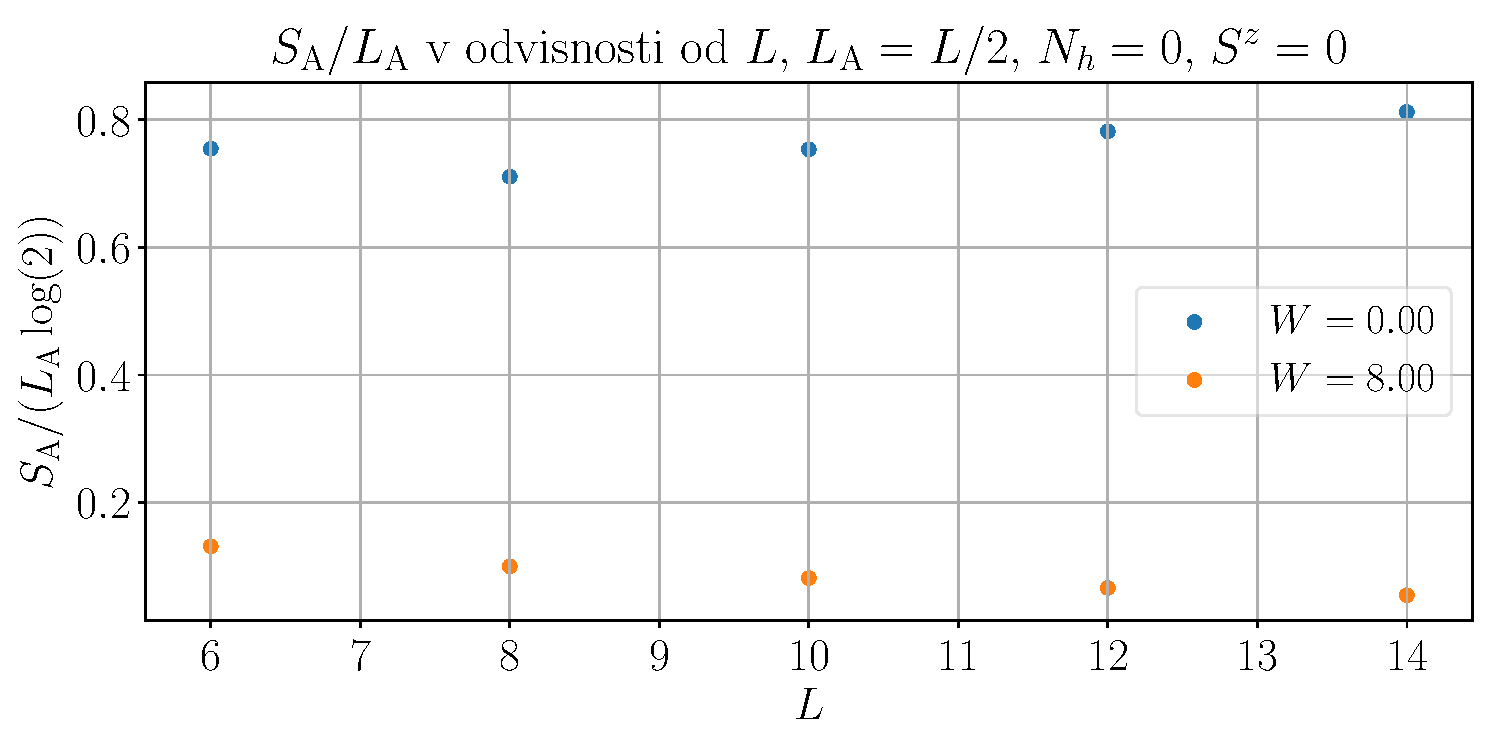
\includegraphics[width=0.7\textwidth]{W_sweep_ent_entropy_scaling_systems_14_0_7.pdf}}
% \caption{Prikaz volumskega in površinskega skaliranja prepletenostne entropije lastnih stanj $S_\mathrm{A}$. 
% Predstavljene so povprečne vrednosti prepletenostne entropije za lastna stanja v sredini pasu.
% Zgoraj: odvisnost prepletenostne entropije od velikosti podsistema $L_\mathrm{A}$ pri fiksni velikosti sistema $L$. Pri volumskem skaliranju $S_\mathrm{A}$ v termodinamski limiti neskončnega sistema narašča sorazmerno z $L_\mathrm{A}$, v primeru površinskega skaliranja pa je $S_\mathrm{A}$ v eni dimenziji za vse velikosti podsistemov enak konstanti. Spodaj: skaliranje prepletenostne entropije pri biparticiji na dva enaka podsistema v odvisnosti od velikosti sistema $L$. V limiti $L\to\infty$ velja v primeru volumskega skaliranja $S_\mathrm{A}/L=\mathrm{const.}$, v primeru površinskega skaliranja pa $S_\mathrm{A}/L=0.$ Izračune smo izvedli za model $t$-$J$ brez vrzeli, ki ustreza izotropnemu Heisenbergovemu modelu z $J=1$.}
% \label{fig:W_sweep_ent_entropy_scaling_systems_14_0_7}
% \end{figure} 

% \begin{figure}[H]
% \floatbox[{\capbeside\thisfloatsetup{capbesideposition={left,center},capbesidewidth=2cm}}]{figure}[\FBwidth]
% {\caption{}\label{fig:H_ent_entro_density_11_5_1}}
% {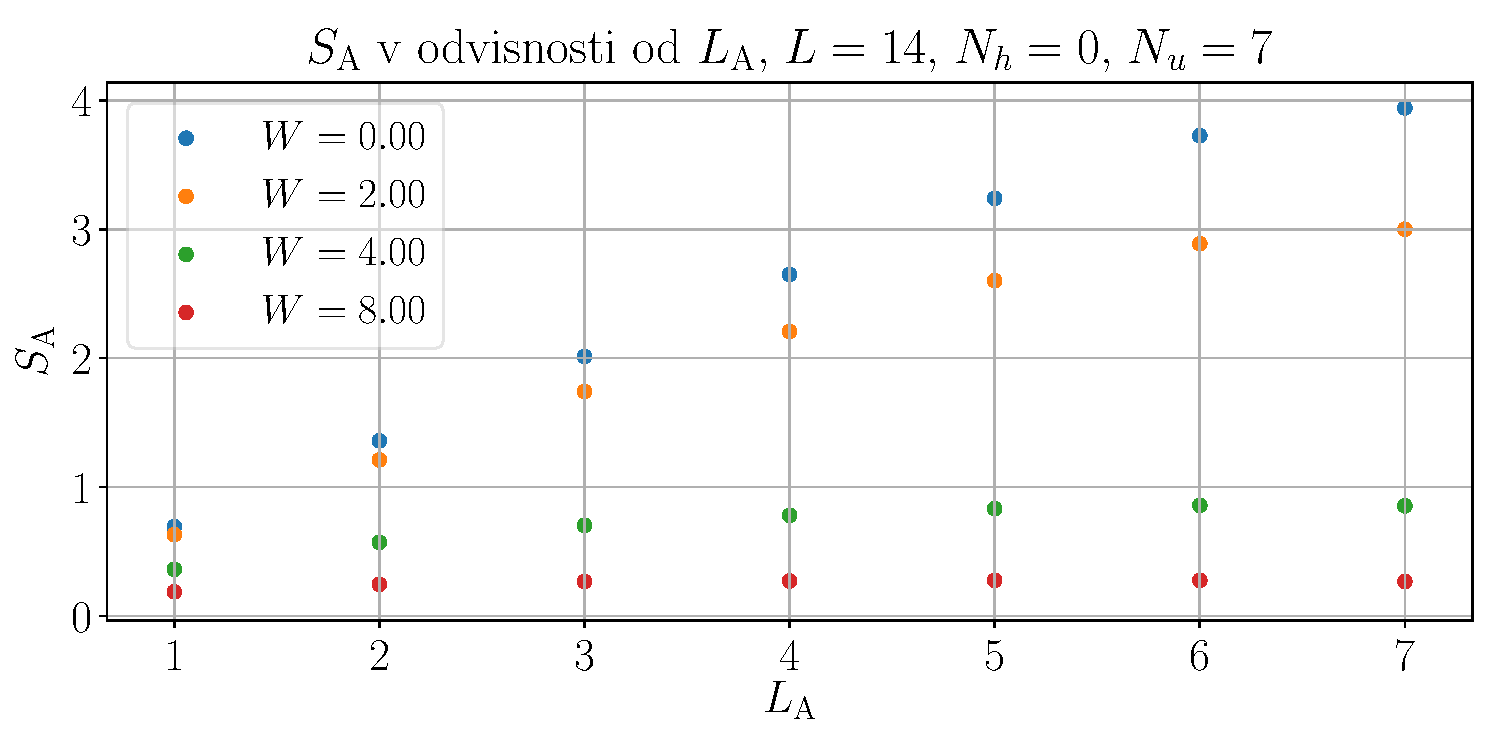
\includegraphics[width=0.6\textwidth]{W_sweep_ent_entropy_scaling_14_0_7.pdf}\\
% 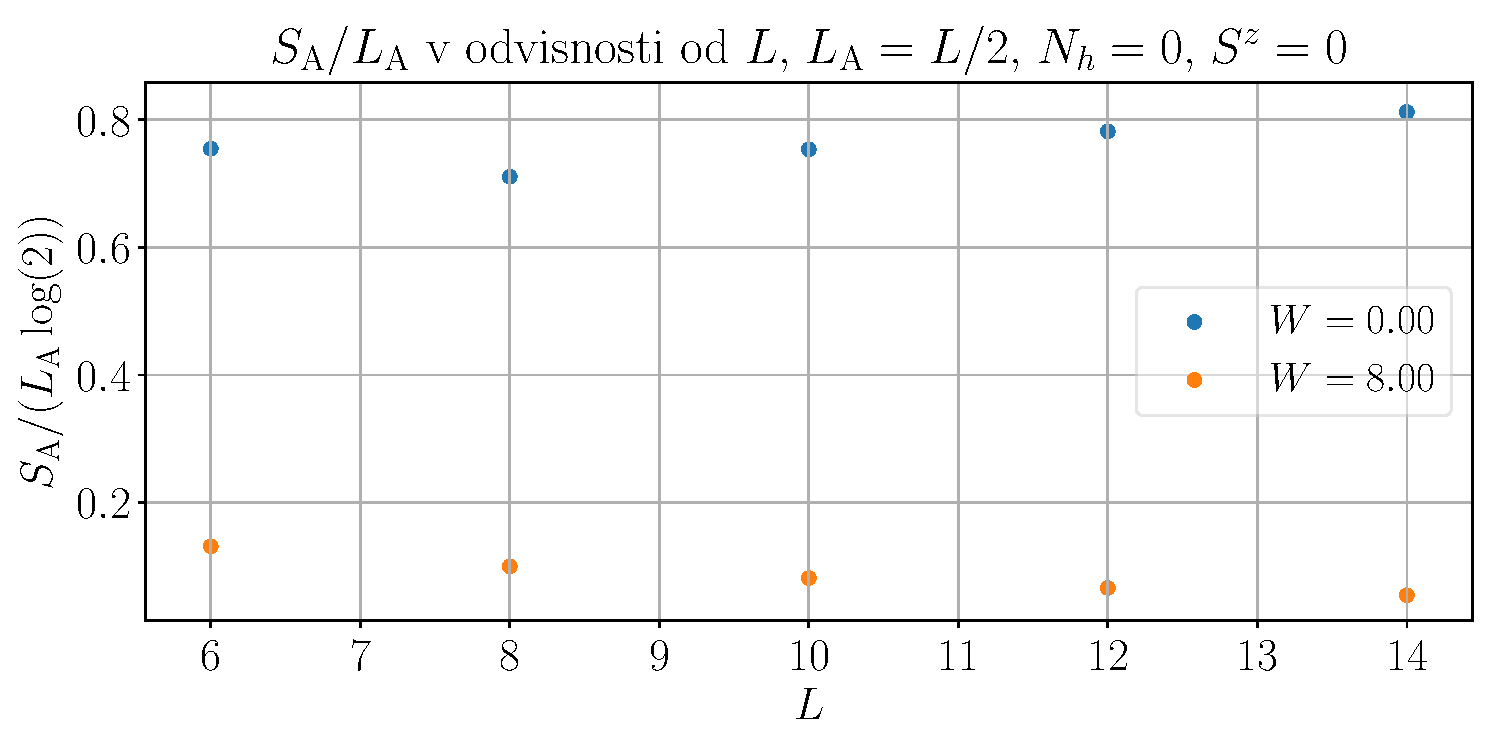
\includegraphics[width=0.6\textwidth]{W_sweep_ent_entropy_scaling_systems_14_0_7.pdf}
% }
% \end{figure}

%  \begin{minipage}[t]{0.25\textwidth}
% \noindent \\
% \end{minipage}\hfill
% \begin{minipage}[t]{0.7\textwidth}
% \begin{figure}[H]
% \centering{
% \includegraphics[width=1\textwidth]{W_sweep_ent_entropy_scaling_14_0_7.pdf}}
% \centering{
% \includegraphics[width=1\textwidth]{W_sweep_ent_entropy_scaling_systems_14_0_7.pdf}}
% \caption{}
% \label{fig:W_sweep_ent_entropy_scaling_systems_14_0_7}
% \end{figure} 
% \end{minipage}

 \begin{figure}[H]
\centering{
\includegraphics[width=1\textwidth]{W_sweep_ent_entropy_density_plot_14_0_7_cuts.pdf}}
\caption{Levo: gostotna ploskev prepletenostne entropije, deljene z maksimalno prepletenostno entropijo podsistema, za vsa lastna stanja pri različnih vrednostih spinskega nereda $W$ za Heisenbergov izotropni model z $J=1$ pri simetrični biparticiji. Rumeni toni ustrezajo ergodični, modri pa MBL fazi. Maksimalna entropija podsistema v Heisenbergovem modelu znaša $L_\mathrm{A}\log(2).$ Ker računamo v bloku s skupnim spinom $S^z=0,$ je število stanj manjše in smo maksimalno entropijo sistema precenili. Z rdečo so označene točke, kjer je dosežena polovična vrednost na intervalu med največjo in najmanjšo izračunano vrednostjo prepletenostne entropije. Desno: prepletenostna entropija vseh lastnih stanj v čistem primeru ob odsotnosti nereda. V tem primeru povprečenje po energijskih intervalih, opisano v besedilu, ni bilo izvedeno.    }
\label{fig:W_ent_entro_density_14_7_0}
\end{figure} 

 \begin{figure}[H]
\centering{
\includegraphics[width=1\textwidth]{W_sweep_ent_entropy_density_plot_11_1_5_cuts.pdf}}
\caption{Izračun prepletenostne entropije v primeru dopiranja z eno vrzeljo in spreminjanja parametra spinskega nereda. V skladu z rezultati, predstavljenimi v poglavju~\ref{statisticne_lastnosti}, opazimo, da spreminjanje parametra spinskega nereda vodi do prehoda med ergodično in lokalizirano fazo. Za velikosti parametra nereda, večje od $W=8$, so namreč vsa stanja v spektru šibko prepletena. }
\label{fig:W_ent_entro_density_11_5_1}
\end{figure} 

 \begin{figure}[H]
\centering{
\includegraphics[width=0.65\textwidth]{H_sweep_ent_entropy_density_plot_11_1_5.pdf}}
\caption{V primeru potencialnega nereda in dopiranja z eno vrzeljo spreminjanje velikosti parametra nereda ne vodi do prehoda v lokalizirano fazo. V nasprotju s primerom s prisotnim spinskim neredom ostanejo stanja na razmeroma širokem energijskem intervalu tudi pri velikem neredu precej prepletena.}
\label{fig:H_ent_entro_density_11_5_1}
\end{figure} 
\newpage

% \begin{figure}[H]
% \floatbox[{\capbeside\thisfloatsetup{capbesideposition={left,center},capbesidewidth=4cm}}]{figure}[\FBwidth]
% {\caption{V primeru potencialnega nereda in dopiranja z eno vrzeljo spreminjanje velikosti parametra nereda ne vodi do prehoda v lokalizirano fazo. V nasprotju s primerom s prisotnim spinskim neredom ostanejo stanja na razmeroma širokem energijskem intervalu tudi pri velikem neredu močno prepletena. }\label{fig:H_ent_entro_density_11_5_1}}
% {\includegraphics[width=0.6\textwidth]{H_sweep_ent_entropy_density_plot_11_1_5.pdf}}
% \end{figure} 

% \begin{figure}[H]
% \centering{
% \includegraphics[width=1\textwidth]{W_sweep_ent_entropy_density_plot_9_3_3_cuts.pdf}}
% \caption{ }
% \label{fig:W_ent_entro_density_9_3_3}
% \end{figure} 

 \begin{figure}[H]
 \centering{
\includegraphics[width=1\textwidth]{W_sweep_ent_entropy_density_plot_9_3_3_cuts.pdf}}
\centering{
\includegraphics[width=0.65\textwidth]{H_sweep_ent_entropy_density_plot_9_3_3.pdf}}
\caption{V primeru tretjinskega dopiranja z vrzelmi rezultati izračuna prepletenostne entropije napovedo možnost prehoda med ergodično in lokalizirano fazo za oba tipa nereda. }
\label{fig:H_ent_entro_density_9_3_3}
\end{figure} 
\noindent
Rezultati izračunov prepletenostne entropije lastnih stanj modela $t$-$J$ so skladni z izračuni spektralnih statistik, predstavljenimi v poglavju~\ref{statisticne_lastnosti}. V primeru dopiranja z eno vrzeljo v prisotnosti spinskega nereda povečevanje parametra nereda vodi do prehoda iz ergodične v lokalizirano fazo, kar za oba tipa nereda velja tudi v primeru tretjinskega dopiranja z vrzelmi. Podobno kot pri izračunu spektralnih statistik tudi pri izračunu prepletenostne entropije za primer ene vrzeli in vrzelnega nereda prehoda iz ergodične v MBL fazo ne zaznamo. 	

\chapter{Zaključek}
V magistrski nalogi smo prisotnost ergodične oziroma MBL faze v preučevanih sistemih analizirali s tremi različnimi statističnimi indikatorji, temelječimi na polni diagonalizaciji modelskih hamiltonk. Pri različnih vrednostih parametrov velikosti nereda smo izračunali povprečno razmerje zaporednih razmikov med energijskimi nivoji $\langle \tilde{r}\rangle$ ter spektralni oblikovni faktor $K(\tau)$ (v nadaljevanju SFF). Medtem ko se prva količina zaradi razmeroma enostavne implementacije v literaturi pogosto uporablja pri presojanju ergodičnosti oziroma lokaliziranosti sistemov, so študije MBL pojavov z uporabo SFF redkejše. Izračuni spektralnih statistik, ki temeljijo na korelacijah med sosednjimi energijskimi nivoji, razkrijejo informacije o obnašanju sistema le na najdaljših časovnih skalah, ki so v komplementarnih študijah časovne dinamike sistemov praviloma nedosegljive. Na drugi strani izračun SFF zaradi upoštevanja korelacij med vsemi energijskimi nivoji v sistemu vključuje vse časovne skale, hkrati pa se rezultati za dolge čase ujemajo z izračuni povprečnega razmerja razmikov med nivoji. Poleg omenjenih spektralnih metod smo ergodičnost oziroma lokaliziranost presojali še na podlagi izračuna prepletenostne entropije vseh lastnih stanj. V nasprotju s spektralnima metodama smo tako dobili tudi informacijo o ergodičnosti oziroma lokaliziranosti posameznih večdelčnih stanj.\\\\
 Osredotočili smo se na model $t$-$J$ v prisotnosti spinskega ter potencialnega nereda za primer dopiranja z eno vrzeljo in primer tretjinskega dopiranja.
 Rezultati vseh treh statističnih indikatorjev v primeru dopiranja z eno vrzeljo ob prisotnosti potencialnega nereda ne kažejo na možnost prehoda v MBL fazo. Za velike vrednosti parametra velikosti potencialnega nereda se vrednost $\langle \tilde{r}\rangle$ ustali pri vrednosti, ki ne ustreza niti Poissonovi niti Wigner-Dysonovi spektralni statistiki. Podobno za velike jakosti potencialnega nereda krivulja SFF ne zavzame konstantne vrednosti, ki bi ustrezala Poissonovi statistiki in bi naznanjala nastop MBL faze. Napovedim na spektralni statistiki temelječih indikatorjev ustrezajo tudi izračuni prepletenostne entropije vseh lastnih stanj sistema, ki pri vseh preučevanih vrednostih nereda kažejo na obstoj znatno prepletenih stanj. V vseh preostalih obravnavanih primerih povečevanje nereda vodi do prehoda med ergodično in lokalizirano fazo, za katero so značilne šibka prepletenost vseh stanj v spektru, vrednost $\langle \tilde{r}\rangle \approx 0.39$ in konstantna vrednost krivulje SFF v univerzalnem režimu, $K(\tau)=1.$ Zaradi hitrega naraščanja dimenzije Hilbertovega prostora z velikostjo sistema v modelu $t$-$J$ smo bili pri izvedbi polne diagonalizacije omejeni na razmeroma majhno število primernih sistemov. Skalirna analiza, s katero bi točneje napovedali vrednosti kritičnih parametrov nereda v termodinamski limiti neskončnega sistema, je pri našem pristopu neizvedljiva, zato so vrednosti parametrov nereda, pri katerih pride do prehoda v naših izračunih, zgolj ocene. Dimenzija največjega preučevanega Hilbertovega prostora je znašala 34650 stanj, in sicer v sistemu z $L=12$ mesti, $N_h=4$ vrzelmi in skupno projekcijo spina $S^z=0.$\\\\
 Tipični modelski sistemi pri preučevanju MBL pojavov so sistemi brezspinskih fermionov in Hubbardove verige. Kolikor nam je znano, zato rezultati za model $t$-$J$, predstavljeni v tem magistrskem delu, še niso bili predhodno izračunani. Podobno velja za samo uporabo izračuna SFF za presojo ergodičnosti oziroma večdelčne lokaliziranosti sistemov. Ne samo, da je bil tovrsten pristop prvikrat uporabljen pri analizi modela $t$-$J$, dosedanjega primera uporabe ne poznamo niti na širšem področju analize MBL pojavov v drugih sistemih. Hkrati s presojo ergodičnosti oziroma večdelčne lokaliziranosti na podlagi ujemanja izračunov z limitinimi napovedmi omogoča izračun SFF tudi vpogled v značilne časovne skale sistema. Vrednost Thoulessovega časa $\tau_\mathrm{H},$ po katerem v odvisnosti $K(\tau)$ ne opazimo več neuniverzalnih pojavov, je pomembna pri preučevanju ergodičnosti na podlagi časovne dinamike tipičnih začetnih stanj. Pristop je komplementaren našemu, $\tau_\mathrm{H}$ pa podaja informacijo o tem, najmanj kako dolg naj bo časovni razvoj, če želimo z njim preučevati ergodičnost oziroma večdelčno lokaliziranost sistema. \\\\
 Medtem ko smo v nalogi izračune za Heisenbergovo spinsko verigo prikazovali le kot ilustrativne zglede ob vpeljavah konceptov SFF in prepletenostne entropije, se zdi sistem primeren za podrobnejšo analizo SFF kot primernega orodja za presojo ergodičnosti oziroma večdelčne lokaliziranosti. Heisenbergova veriga namreč omogoča bistveno lažjo izvedbo skalirne analize, hkrati pa je možna tudi primerjava izračunov z že znanimi napovedmi drugih metod. Drugo izhodišče za prihodnje raziskave je vpeljava mikrokanonične različice izračuna SFF, s katero bi namesto lastnosti celotnega spektra slednje preučevali le v ozkem energijskem oknu. Ker bi v energijskem oknu morali zagotoviti zadostno število stanj, bi to terjalo preučevanje večjih sistemov. Posledično izračun lastnih stanj ne bi več temeljil na polni diagonalizaciji, medtem ko bi sam postopek izračuna SFF na dobljenem spektru ostal  enak postopku, predstavljenem v tem magistrskem delu. 
\cleardoublepage\phantomsection
\addcontentsline{toc}{chapter}{Literatura}
\bibliographystyle{fmf-sl}
\bibliography{literatura}

%%% DODATKI

\cleardoublepage
\renewcommand\appendixname{Dodatek}
\begin{appendices}

\chapter{Preslikava med Hubbardovim modelom in modelom $t$-$J$}
\label{tj_hubb_preslikava}
Zanima nas izpeljava preslikave med Hubbardovim modelom in modelom $t$-$J$, pri čemer želimo obravnavati tudi vpliv potencialnega nereda, ki se sklaplja bodisi z nosilci naboja bodisi s spini. Uvodoma obravnavamo enostavnejši primer brez dodatnega naključnega nereda, v drugem delu pa vključimo tudi tega. 
\section{Primer brez nereda}
Obravnavamo Hubbardov model, ki ga v približku tesne vezi podaja hamiltonka
\begin{equation}\label{eq:hubbard}
H=H_t + H_U=-t\sum\limits_{\langle ij \rangle, \sigma}\left(c^\dagger_{i,\sigma} c_{j\sigma} + c^\dagger_{j\sigma}c_{i\sigma}\right) + U\sum_i n_{i\uparrow}n_{i\downarrow}.
\end{equation}
Pri tem  $\langle ij \rangle$ označuje vsoto po najbližjih sosedih, $\sigma$ pa vsoto po projekcijah spina na os $z$. Fermionski kreacijski in anihilacijski operatorji $c^\dagger_{i,\sigma}, c_{i,\sigma}$ ustvarijo oziroma uničijo delec z dano projekcijo spina $\sigma$ na $i$-tem mestu v kristalni rešetki.  Med izpeljavo bomo pri zapisu večdelčnih stanj upoštevali naslednjo ureditev fermionskih operatorjev
$$
\ket{\psi}=\prod\limits_{\{i_\uparrow \}} c_{i, \uparrow}^\dagger \prod\limits_{\{j_\downarrow \}} c_{j, \downarrow}^\dagger \ket{0},
$$
kjer je $\ket{0}$ vakuumsko stanje, produkta pa tečeta po vseh mestih, na katerih se nahajajo spini z dano projekcijo. \\\\
V hamiltonki, ki jo podaja En. \eqref{eq:hubbard}, skakalni člen $H_t$ opisuje skakanje elektronov med sosednjimi mesti v kristalni rešetki, pri čemer je $t$ verjetnost za tovrstno tuneliranje. Interakcijski člen $H_U$ modelira coulombski odboj med elektroni in ob dvojni zasedenosti mesta povzroči energijski prirastek $U$. V limitnem primeru $t\to 0$, oziroma v limiti popolnoma lokaliziranih enodelčnih valovnih funkcij, so večdelčna stanja brez dvojne zasedenosti mest medsebojno degenerirana pri ničelni energiji. Pri izpeljavi modela $t$-$J$ predpostavimo močno coulombsko interakcijo $U$ in posledično nizko koncentracijo energijsko neugodnih dvojno zasedenih mest. V tem primeru so visokoenergijska stanja z dvojno zasedenimi mesti v energijskem spektru dobro ločena od stanj z največ enojno zasedenimi mesti. Za opis nizkoenergijskih stanj Hubbardove hamiltonke, podane z En. \eqref{eq:hubbard}, torej v tej limiti zadošča obravnava problema na podprostoru največ enojno zasedenih stanj.  \\
Preslikavo med Hubbardovim modelom in modelom $t$-$J$ bomo izpeljali perturbativno, začenši v limiti popolnoma lokaliziranih enodelčnih valovnih funkcij, kjer kot neperturbirani del hamiltonke vzamemo interakcijski člen $H_t$, kinetični člen $H_U$ pa vključimo kot perturbacijo. Zanima nas oblika efektivne hamiltonke $\tilde{H}$, s katero v limiti močne coulombske interakcije opišemo fiziko nizkoenergijskih stanj Hubbardove hamiltonke. Ker se v slednji sklapljajo le sosednja mesta, lahko problem brez škode za splošnost obravnavamo na dveh sosednjih mestih. Ob upoštevanju prepovedi dvojne zasedenosti mest razpenjajo bazo pripadajočega Hilbertovega podprostora naslednja stanja:
%\begin{equation}
%\begin{aligned}\qquad
%&\ket{\alpha_1}= \ket{  \overset{i}{\uparrow} \overset{j}{\uparrow}}=c^\dagger_{i,\uparrow}c^\dagger_{j,\uparrow}\ket{0} & \ket{\alpha_2}=\ket{ \downarrow \downarrow}=c^\dagger_{i,\downarrow}c^\dagger_{j,\downarrow}\ket{0},\hspace{5mm} &\ket{\alpha_5}= \ket{\uparrow \bullet}=c^\dagger_i\ket{0} &\ket{\alpha_6}=\ket{ \bullet  \uparrow}=c^\dagger_{j,\uparrow}\ket{0}\\
%&\ket{\alpha_3}=\ket{ \uparrow \downarrow }=c^\dagger_{i,\uparrow}c^\dagger_{j,\downarrow}\ket{0} &\ket{\alpha_4}=\ket{ \downarrow \uparrow }=c^\dagger_{j,\uparrow}c^\dagger_{i,\uparrow}\ket{0},\hspace{5mm} &\ket{\alpha_7}=\ket{\downarrow \bullet}=c^\dagger_j\ket{0}&\ket{\alpha_8}=\ket{ \bullet  \downarrow }=c^\dagger_{j,\downarrow}\ket{0}\\\\
%\end{aligned}
%\end{equation}
\begin{equation}\label{eq:stanja}
\begin{aligned}\qquad
&\ket{\alpha_1}= \ket{  \overset{i}{\uparrow} \overset{j}{\uparrow}}=c^\dagger_{i,\uparrow}c^\dagger_{j,\uparrow}\ket{0} & \ket{\alpha_2}=\ket{ \downarrow \downarrow}=c^\dagger_{i,\downarrow}c^\dagger_{j,\downarrow}\ket{0}\\
&\ket{\alpha_3}=\ket{ \uparrow \downarrow }=c^\dagger_{i,\uparrow}c^\dagger_{j,\downarrow}\ket{0} &\ket{\alpha_4}=\ket{ \downarrow \uparrow }=c^\dagger_{j,\uparrow}c^\dagger_{i,\uparrow}\ket{0} \\\\
&\ket{\alpha_5}= \ket{\uparrow \bullet}=c^\dagger_{i,\uparrow}\ket{0} &\ket{\alpha_6}=\ket{ \bullet  \uparrow}=c^\dagger_{j,\uparrow}\ket{0}\\
&\ket{\alpha_7}=\ket{\downarrow \bullet}=c^\dagger_{j,\downarrow}\ket{0}&\ket{\alpha_8}=\ket{ \bullet  \downarrow }=c^\dagger_{j,\downarrow}\ket{0}\\
\end{aligned}
\end{equation}
Označimo podprostor stanj brez vrzeli z $\{ \ket{\alpha^0}\}$ in podprostor stanj z vrzeljo $\{ \ket{\alpha^1}\}$.
Prepovedana stanja z energijo $U$ in dvojno zasedenostjo mest bomo potrebovali pri perturbacijski obravnavi in jih zapišemo  kot 
\begin{equation}\label{eq:vzbujena}
\ket{\beta}=\ket{ \overset{i}{\uparrow\downarrow}\overset{j}{\bullet}}=c^\dagger_{i,\uparrow}c^\dagger_{i,\downarrow}\ket{0}, \hspace{10mm} 
\ket{\beta'}=\ket{\overset{i}{\bullet}\overset{j}{\uparrow\downarrow}}=c^\dagger_{j,\uparrow}c^\dagger_{j,\downarrow}\ket{0}.
\end{equation}
 V modelu $t$-$J$ so skoki delcev med posameznimi mesti dovoljeni le v primeru, ko je na ciljnem mestu pred skokom vrzel. Formalno zahtevi zadostimo z uvedbo projiciranih fermionskih operatorjev $\tilde{c}_{i\sigma}$ v skladu s predpisom 
\begin{equation}\label{eq:projicirani}
\tilde{c}^\dagger_{i\sigma}= c^\dagger_{i\sigma} \left(1-n_{i-\sigma}\right),
\end{equation}
s čimer preprečimo možnost dvojne zasedenosti posameznega mesta. Kinetični del $\tilde{H}_\mathrm{kin}$ efektivne hamiltonke $\tilde{H}$ tako dobimo v prvem redu perturbacije z delovanjem operatorja $H_\mathrm{kin}$ na podprostoru $\{ \ket{\alpha^1} \}$. S projiciranimi operatorji ga zapišemo kot 
\begin{equation}\label{eq:ef_kin}
\tilde{H}_t=-t\sum\limits_{\langle ij \rangle \sigma} \left(\tilde{c}^\dagger_{i,\sigma} \tilde{c}_{j\sigma} + \tilde{c}^\dagger_{j\sigma}\tilde{c}_{i\sigma}\right).
\end{equation}
Pri nadaljnji perturbacijski obravnavi moramo upoštevati drugi red degenerirane perturbacijske teorije, saj v podprostoru $\{ \ket{\alpha^0}\}$ direktni matrični elementi $\bra{\alpha} H_t \ket{\alpha}$ ne obstajajo, vsa stanja $\ket{\alpha}$ pa so ob odsotnosti perturbacije degenerirana. 
Matrične elemente efektivne hamiltonke v tem primeru podaja zveza 
\begin{equation}
\left(\tilde{H}_\mathrm{eff}\right)_{\alpha, \alpha'}=\sum\limits_{\beta\neq\alpha}\frac{\bra{\alpha}H_t\ket{\beta}\bra{\beta}H_t\ket{\alpha'}}{E_\alpha^0 - E_\beta^0},
\end{equation}
kjer vsota teče po vzbujenih stanjih, podanih z En. \eqref{eq:vzbujena}. Hitro vidimo, da je 
$H_t\ket{\beta}=H_t\ket{\beta'}=-t\left(\ket{\alpha_3}+ \ket{\alpha_4}\right)$ in da so potemtakem neničelni le matrični elementi $\tilde{H}_{33}=\tilde{H}_{44}=\tilde{H}_{34}=\tilde{H}_{43}=-\frac{2t^2}{U}$. Tu smo upoštevali $E_\alpha^0- E_\beta^0 \sim -U$. Če zapišemo matrične elemente $\tilde{H}_\mathrm{eff}$ kot
\begin{equation}
\begin{aligned}\qquad
&\tilde{H}_{33}=\ket{\alpha_3}\bra{\alpha_3}=\frac{-2t^2}{U} c^\dagger_{i,\uparrow}c^\dagger_{j,\downarrow}c_{j,\downarrow}c_{i,\uparrow}= \frac{2t^2}{U}c^\dagger_{i,\uparrow}c_{i,\uparrow}c^\dagger_{j,\downarrow}c_{j,\downarrow},\\
&\tilde{H}_{44}=\ket{\alpha_4}\bra{\alpha_4}=\frac{-2t^2}{U} c^\dagger_{j,\uparrow}c^\dagger_{i,\downarrow}c_{i,\downarrow}c_{j,\uparrow}= \frac{2t^2}{U}c^\dagger_{j,\uparrow}c_{j,\uparrow}c^\dagger_{i,\downarrow}c_{i,\downarrow},\\
&\tilde{H}_{34}=\ket{\alpha_3}\bra{\alpha_4}=\frac{-2t^2}{U} c^\dagger_{i,\uparrow}c^\dagger_{j,\downarrow}c_{i,\downarrow}c_{j,\uparrow}= \frac{2t^2}{U}c^\dagger_{i,\uparrow}c_{i,\downarrow}c^\dagger_{j,\downarrow}c_{j,\uparrow},\\
&\tilde{H}_{43}=\ket{\alpha_4}\bra{\alpha_3}=\frac{-2t^2}{U} c^\dagger_{j,\uparrow}c^\dagger_{i,\downarrow}c_{j,\downarrow}c_{i,\uparrow}= \frac{2t^2}{U}c^\dagger_{j,\uparrow}c_{j,\downarrow}c^\dagger_{i,\downarrow}c_{i,\downarrow},
\end{aligned}
\end{equation}
potem lahko  $\tilde{H}_\mathrm{eff}$ zapišemo kot 
\begin{equation}\label{eq:efektivno}
\tilde{H}_\mathrm{eff} = \frac{2t^2}{U}\sum\limits_{\langle ij\rangle \sigma } \left[\tilde{c}^\dagger_{i,\sigma}\tilde{c}_{i,-\sigma}\tilde{c}^\dagger_{j,-\sigma}\tilde{c}_{j,\sigma} + n_{i,\sigma}n_{j,-\sigma}  \right].
\end{equation}
En. \eqref{eq:efektivno} lahko prikladneje zapišemo z uporabo spinskih operatorjev. Prepoznamo namreč $S_i^+=\tilde{c}^\dagger_{i,\uparrow}\tilde{c}_{i,\downarrow}$ in $S_i^-=\tilde{c}^\dagger_{i,\downarrow}\tilde{c}_{i,\uparrow}$, pri zapisu $\sum\limits_{\sigma} n_{i,\sigma}n_{j,-\sigma}$ pa uporabimo zvezi $n_i=\left( n_{i,\uparrow} + n_{i, \downarrow}\right)$ in $S_i^z=\frac{1}{2}\left(n_{i, \uparrow} - n_{i, \downarrow} \right)$. Dobimo
\begin{equation}\label{eq:mat_elti}
\begin{split}
\tilde{H}_\mathrm{eff}& = \frac{2t^2}{U} \sum\limits_{\langle ij \rangle}\left[ \left( S_i^+S_j^- + S_i^-S_j^+\right) - \frac{n_i n_j - 4S_i^zS_j^z}{2}\right]=\\
&=J\sum\limits_{\langle ij \rangle} \left[ \vec{S}_i\cdot  \vec{S}_j - \frac{n_i n_j}{4}\right].
\end{split}
\end{equation}
Pri tem smo vpeljali izmenjalno sklopitev $J=\frac{4t^2}{U}$, na vmesnem koraku zgornje izpeljave pa smo uporabili enakost $2S_i\cdot S_j = 2S_i^z S_j^z + S_i^+S_j^+ + S_i^-S_j^+$. Celotna hamiltonka $\tilde{H}$ se ob upoštevanju mobilnih vrzeli in sklopitve magnetnih prostostnih stopenj zapiše kot 
\begin{equation}\label{eq:tjhamiltonka}
\tilde{H} = -t\sum\limits_{\langle ij \rangle \sigma} \left(\tilde{c}^\dagger_{i,\sigma} \tilde{c}_{j\sigma} + \tilde{c}^\dagger_{j\sigma}\tilde{c}_{i\sigma}\right) +  J\sum\limits_{\langle ij \rangle} \left[ \vec{S}_i\cdot  \vec{S}_j - \frac{n_i n_j}{4}\right]
\end{equation}
Pri izpeljavi nismo upoštevali prispevkov drugega reda zaradi sklopitve mesta z levim in desnim sosedom, ki vodijo do t.i.~\emph{koreliranega skakanja.}
\section{Dodatek nereda}
Tokrat nas zanima, na kateri tip nereda v modelu $t$-$J$ se preslika nered, ki ga v Hubbardovem modelu sklopimo bodisi s spini bodisi z vrzelmi. Hamiltonki, ki jo podaja En. \eqref{eq:hubbard}, v vsej splošnosti dodamo člen z neredom kot 
\begin{equation}
H=H_t + H_U + H_\mathrm{dis}=-t\sum\limits_{\langle ij \rangle, \sigma}\left(c^\dagger_{i,\sigma} c_{j\sigma} + c^\dagger_{j\sigma}c_{i\sigma}\right) + U\sum_i n_{i\uparrow}n_{i\downarrow} + \sum\limits_{i,\sigma} h_{i,\sigma} n_{i, \sigma}  
\end{equation}
kjer so $h_{i,s}$ v skladu z neko verjetnostno porazdelitvijo izžrebane naključne vrednosti, pri čemer sta porazdelitvi za posamezni projekciji spina v splošnem lahko različni. V prvem redu perturbacije dobimo za kinetični člen in člen z neredom naslednji izraz
\begin{equation}
\tilde{H}_\mathrm{kin} + \tilde{H}_\mathrm{dis} = -t\sum\limits_{\langle ij \rangle \sigma} \left(\tilde{c}^\dagger_{i,\sigma} \tilde{c}_{j\sigma} + \tilde{c}^\dagger_{j\sigma}\tilde{c}_{i\sigma}\right) +\sum\limits_{i,\sigma} h_{i,\sigma} \left(1-n_{i,-\sigma}\right)n_{i,\sigma}
\end{equation}
Na mestih $i, j$ smo tako dodali nered $h_{\{i,j\},\sigma}$. Stanji $\ket{\beta}$ in $\ket{\beta'}$ imata sedaj energiji 
\begin{equation}
E_\beta = U + h_{i,\uparrow} + h_{i,\downarrow}, \hspace{5mm} E_{\beta'}= U + h_{j, \uparrow} + h_{j,\downarrow} 
\end{equation}
za uporabo perturbacijske teorije drugega reda pa potrebujemo bazo medsebojno degeneriranih stanj. Iz stanj, podanih v En. \eqref{eq:stanja}, sestavimo bazo 
\begin{equation}
\begin{split}
%\ket{\tilde{\alpha}_1}=&\frac{1}{\sqrt{2}}\left( \ket{\alpha_1 } + \ket{\alpha_2}\right), \hspace{5mm} \ket{\tilde{\alpha}_2}= \frac{1}{\sqrt{2}}\left(\ket{\alpha_1 } - \ket{\alpha_2}\right)\\
\ket{\tilde{\alpha_3}}=&\frac{1}{\sqrt{2}}\left( \ket{\alpha_3} + \ket{\alpha_4}\right), \hspace{ 5mm}\ket{\tilde{\alpha_4}}=\frac{1}{\sqrt{2}}\left(\ket{\alpha_3} - \ket{\alpha_4}\right).
\end{split}
\end{equation}
Od prej vemo, da stanji $\ket{\alpha_1}$ in $\ket{\alpha_2}$ za našo izpeljavo nista pomembni, saj bosta prispevali le ničelne matrične elemente v efektivni hamiltonki, medtem ko sta zgornji stanji ob odsotnosti perturbacije degenerirani z energijo $$E_0^\alpha= \frac{1}{2} \left(h_{i,\uparrow} + h_{i,\downarrow} + h_{j,\uparrow} + h_{j,\downarrow}\right).$$ Takoj vidimo, da je 
$H_\mathrm{kin}\ket{\beta}= H_\mathrm{kin}\ket{\beta'}=-t\left(\ket{\alpha_3}+\ket{\alpha_4}\right)=-t\sqrt{2} \ket{\tilde{\alpha}_3}$. V efektivni hamiltonki imamo tako samo člen 
$$\tilde{H}_{\tilde{3},\tilde{3}}=2t^2\left(\frac{1}{U - \Xi_{i,j}} + \frac{1}{ U + \Xi_{i,j}}\right), $$
kjer je 
\begin{equation}\label{eq:izpeljava_vpeljava_xi}
\Xi_{i,j}=\frac{1}{2}\sum\limits_\sigma \left(h_{i,\sigma} - h_{j,\sigma}\right).
\end{equation}
V bazi stanj $\ket{\alpha_3}, \ket{\alpha_4}$ imamo tako 
$$
\tilde{H}_{3,3}=\tilde{H}_{4,4}=\tilde{H}_{3,4}=\tilde{H}_{4,3}=t^2\left( \frac{1}{U - \Xi_{i,j}} + \frac{1}{U + \Xi_{i,j}}\right).
$$
Od tu naprej je razprava enaka kot zgoraj, zaradi vpliva nereda očitno postane tudi sklopitvena konstanta krajevno odvisna, $J\rightarrow J_{i,j}$, kjer je 
\begin{equation}
J_{i,j}=2t^2 \left( \frac{1}{U-\Xi_{i,j}} + \frac{1}{U+ \Xi_{i,j}}\right).
\end{equation}
V odsotnosti nereda pridemo nazaj v predhodni primer, $J=\frac{4t^2}{U}$. Z dodatkom nereda se tako Hubbardova hamiltonka, podana z En. \eqref{eq:hubbard}, v hamiltonko modela $t$-$J$ preslika kot 
\begin{equation}
\tilde{H}=-t\sum\limits_{\langle ij \rangle \sigma} \left(\tilde{c}^\dagger_{i,\sigma} \tilde{c}_{j\sigma} + \tilde{c}^\dagger_{j\sigma}\tilde{c}_{i\sigma}\right) +\sum\limits_{\langle ij \rangle} J_{i,j}\left[ \vec{S}_i\cdot  \vec{S}_j - \frac{n_i n_j}{4}\right] +\sum\limits_{i,\sigma} h_{i,\sigma} \left(1-n_{i,-\sigma}\right)n_{i,\sigma}.
\end{equation}
V tem magistrskem delu privzamemo, da je $J$ konstanten, $J_{i,j}=J.$ Vrzelni in spinski nered lahko uvedemo kot ustrezno linearno kombinacijo členov $h_{i,\uparrow}$ in $h_{i,\downarrow}.$ Spinski nered ustreza izbiri
\begin{equation}\label{eq:izpeljava_vpeljava_spinski}
h_{i,\uparrow}=-h_{i,\downarrow},
\end{equation}
vrzelni nered pa izbiri 
\begin{equation}\label{eq:izpeljava_vpeljava_vrzelni}
h_{i,\uparrow}=h_{i,\downarrow}.
\end{equation}
Iz En.~\eqref{eq:izpeljava_vpeljava_xi} lahko razberemo, da uvedba spinskega nereda ne vpliva na vrednost izmenjalne konstante, saj je $\Xi_{i,j}$ v tem primeru enak nič. Možne so tudi vpeljave drugih tipov nereda, denimo takšnega, ki se sklaplja zgolj z eno vrsto spinov, v tem primeru izžrebamo $h_{i,\sigma}$ in postavimo $h_{i,-\sigma}=0.$ 
% \section{Numerična primerjava}
% Na Sliki~\ref{fig:diffs_graph} so prikazani rezultati numerične primerjave 
% \begin{figure}[H]
% \centering{
% \includegraphics[width=1.\textwidth]{diffs_graph.pdf}}
% \caption{}
% \label{fig:diffs_graph}
% \end{figure}
\end{appendices}


%%% KAZALO (NEOBVEZNO)

\cleardoublepage
\printindex

\end{document}



